%% wm-pln-book: WM-PLN — The World-Model Calculus
%%
%% Render with:
%%   lualatex -shell-escape wm-pln-book.tex && bibtex wm-pln-book && lualatex -shell-escape wm-pln-book.tex && lualatex -shell-escape wm-pln-book.tex

\documentclass[11pt,openany]{report}
\usepackage{pln-common}
\usepackage{tikz}
\usepackage{url}
\usetikzlibrary{arrows.meta,positioning,calc,decorations.pathreplacing}

\title{WM-PLN:\\[4pt]
  The World-Model Calculus\\[12pt]
  \large\texttt{(DRAFT --- \today)}}
\author{Zar and Oru\v{z}i\thanks{%
  Oru\v{z}i denotes AI-assisted collaboration using ChatGPT, Codex, and Claude Code.}}
\date{}

\begin{document}
\maketitle

\begin{abstract}
Probabilistic Logic Networks (PLN) couples logical structure with uncertain
inference.  In practice, however, many PLN presentations mix three distinct
layers: (i)~a probabilistic world-model posterior, (ii)~an evidence algebra
for compositional aggregation, and (iii)~operational truth-value views
(strength, confidence, interval bounds).  This conflation produces
\emph{semantic drift}: algebraic operators are treated as if they were the
logic itself, and link-level inference attempts to propagate
correlation-sensitive quantities without carrying the information required to
do so correctly.

We present the \emph{world-model calculus}, the mathematical foundation
underlying \xiPLN{}\footnote{Informally also $\Omega$-PLN, after the
world space~$\Omega$ that anchors every definition in the calculus.},
designed to be (a)~correct by construction and
(b)~extensible to tractable sublayers.  The core move is to make the
complete layer a \emph{posterior-state calculus}: the proof object is a
revisable world-model posterior state, and all truth values are obtained
by querying that state.  We give a reference complete
instance as a Dirichlet posterior over complete worlds (\JointEvidence{}),
prove that evidence extraction commutes with revision, and formalize a no-go
theorem showing that complete link evidence cannot, in general, be computed
from local per-link evidence alone.  We then show how Bayesian-network-style
sublayers, higher-order reductions, quantifier semantics, intensional
inheritance, and inference-control theory arise as compiled tactics with
explicit assumptions within the world-model framework.

All results are formalized in Lean~4 with Mathlib, totaling over 500
theorem-backed modules across evidence algebra, world-model calculus,
compiled BN inference, higher-order chaining, and applied
demonstrations.
\end{abstract}

\tableofcontents

%% ═══════════════════════════════════════════════════════════════════
\part{Orientation}
\label{part:orientation}
%% ═══════════════════════════════════════════════════════════════════

\chapter{Introduction}
\label{ch:introduction}

\begin{quote}\small
\textbf{Goal:} Diagnose semantic drift in PLN and motivate the world-model refoundation.\\
\textbf{Semantic object:} Three-layer architecture (world model, evidence algebra, views).\\
\textbf{Proved:} Nothing (orientation chapter).\\
\textbf{Assumed:} Familiarity with basic probability; PLN book familiarity helpful but not required.
\end{quote}

Probabilistic Logic Networks, as described by Ben Goertzel, Matthew Ikl\'{e},
Izabela Freire Goertzel, and Ari Heljakka~\cite{goertzel2009pln}, represent uncertain judgments using truth
values: a \emph{strength} (probability-like estimate) and a \emph{confidence}
(reliability-like quantity derived from sample size).  The ambition was
generous---to build a general-purpose uncertain reasoner capable of deduction,
induction, abduction, and revision, all within a unified algebraic framework.

That ambition produced real insights.  The evidence-count representation, the
separation of strength from confidence, the recognition that revision must be
compositional, and the aspiration to connect logical structure with
probabilistic semantics---these were the right instincts.  But in the passage
from intuition to formalization, something went wrong.

\section{Where Semantic Drift Came From}

The difficulty is not that PLN's rules are wrong.  Many of them are
correct---under assumptions that were left implicit.  The difficulty is that
the original presentation mixes three conceptually distinct layers without
always marking where one ends and another begins:

\begin{enumerate}
\item \textbf{The world-model layer.}  A probabilistic model---a joint
  distribution, a Bayesian network, or some structured posterior---that can
  answer any query by conditioning.  This is the \emph{complete} semantics.

\item \textbf{The evidence-algebra layer.}  An algebraic structure on
  observation counts $(n^+, n^-)$ with revision as addition, information
  ordering, and lattice operations.  This is a \emph{compositional bookkeeping}
  layer.

\item \textbf{The operational-view layer.}  Strength, confidence, weight,
  interval bounds---these are \emph{extracted summaries} of evidence, useful for
  thresholding, display, and approximate computation, but not themselves the
  semantics.
\end{enumerate}

\begin{figure}[htbp]
\centering
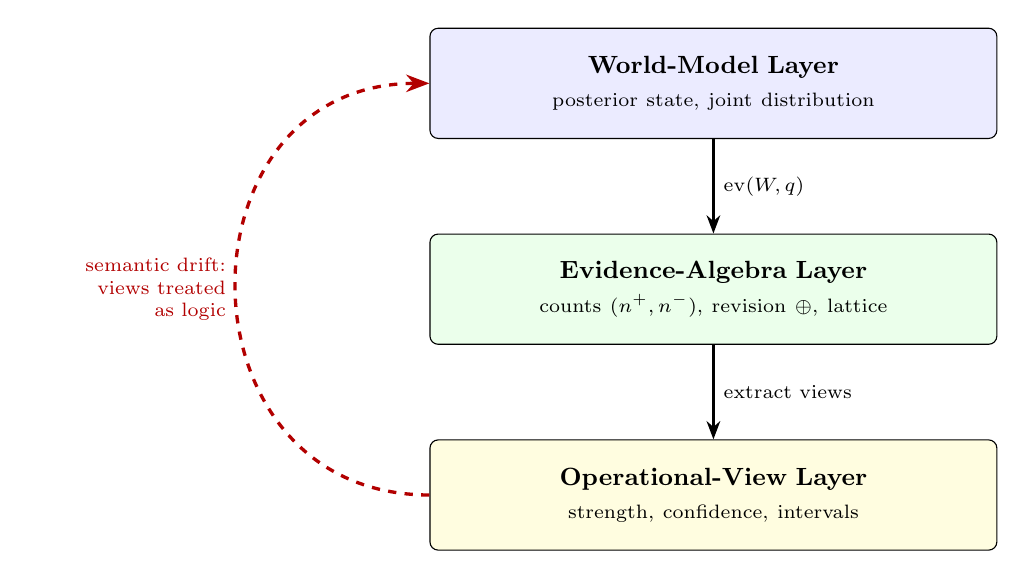
\begin{tikzpicture}[
  >=Stealth,
  every node/.style={font=\small},
  layer/.style={draw, rounded corners=3pt, minimum width=72mm, minimum height=14mm,
                align=center, text width=68mm},
]
\node[layer, fill=blue!8] (wm)
  {{\bfseries World-Model Layer}\\[1pt]
   {\scriptsize posterior state, joint distribution}};
\node[layer, fill=green!8, below=12mm of wm] (ev)
  {{\bfseries Evidence-Algebra Layer}\\[1pt]
   {\scriptsize counts $(n^+,n^-)$, revision $\oplus$, lattice}};
\node[layer, fill=yellow!12, below=12mm of ev] (view)
  {{\bfseries Operational-View Layer}\\[1pt]
   {\scriptsize strength, confidence, intervals}};

% correct downward flow
\draw[->, thick] (wm) -- node[right, font=\scriptsize] {$\mathrm{ev}(W,q)$} (ev);
\draw[->, thick] (ev) -- node[right, font=\scriptsize] {extract views} (view);

% semantic drift: red dashed arrow bypassing the middle
\draw[->, dashed, very thick, red!70!black]
  (view.west) to[out=180, in=180, looseness=1.6]
  node[left, font=\scriptsize, text width=24mm, align=right]
    {semantic drift:\\views treated\\as logic}
  (wm.west);
\end{tikzpicture}
\caption{The three-layer architecture of \xiPLN{}.  Solid arrows show the
correct information flow: query the world model for evidence, then extract
operational views.  The dashed red arrow marks the conflation that produces
semantic drift---treating views as if they were the complete semantics.}
\label{fig:three-layer-architecture}
\end{figure}

\paragraph{Orientation example: the Home Helper.}
To make these layers concrete, consider a home-assistant system managing
comfort and safety in a small apartment.  Rooms (\emph{Kitchen},
\emph{Bedroom}) contain sensors (\emph{TempSensor}, \emph{HumiditySensor},
\emph{MotionSensor}) and devices (\emph{Heater}, \emph{Window},
\emph{Dehumidifier}).  The latent states of interest are
\emph{WindowLeaking}, \emph{RoomOccupied}, and \emph{HeaterWorking}.

\begin{itemize}
\item \textbf{World-model layer:} a small Bayesian network linking latent
  states to sensor readings: $\mathrm{WindowLeaking} \to \mathrm{HumidityHigh}$,
  $\mathrm{HeaterWorking} \to \mathrm{TempHigh}$,
  $\mathrm{RoomOccupied} \to \mathrm{MotionDetected}$.
\item \textbf{Evidence layer:} temperature readings are Normal-Gamma evidence
  (continuous); motion detections are Beta evidence (binary); humidity is
  Dirichlet evidence (multi-valued: low/medium/high).
\item \textbf{View layer:} ``Is the window likely leaking?'' extracts a
  strength and confidence from the posterior.  ``Should I turn on the
  heater?'' uses the exceedance query $P(T_{\mathrm{new}} < 18°\mathrm{C})$.
\end{itemize}

This scenario exercises evidence aggregation (Ch.~\ref{ch:evidence}),
distributional semantics (Ch.~\ref{ch:distributional}), BN compiled
inference (Ch.~\ref{ch:bn-models}), temporal filtering
(Ch.~\ref{ch:temporal}), and drift/recalibration---all themes developed
in subsequent chapters.  Semantic drift would occur if, for example,
the system chained strength values through the window$\to$humidity$\to$mold
path without tracking the variance lost at each step.

When these layers are conflated, several things go wrong.  Operational views
get treated as if they \emph{were} the logic: interval bounds are composed
with rules designed for point probabilities, confidence heuristics are chained
without tracking what information they lost.  Link-level inference attempts to
compute complete posteriors from local link truth values, ignoring the
correlations that live only in the joint state.  The result is semantic drift:
the system \emph{almost} works, but its correctness depends on assumptions
that are neither stated nor checked.

\section{What the Refoundation Changes}

\xiPLN{} is a response to semantic drift.  It does three things:

\begin{enumerate}
\item It makes the \emph{world-model posterior state} the primary proof object.
  Inference does not propagate truth values between links; it revises posterior
  states and answers queries against the revised state.

\item It isolates the \emph{evidence algebra} as a separate, well-defined
  algebraic layer---a quantale and Heyting frame on observation counts---that
  serves compositional aggregation but does not pretend to be the complete
  semantics.

\item It treats all classic PLN rules (deduction, induction, abduction,
  revision) as \emph{compiled tactics}: derived rewrites that are correct
  under explicit side conditions within declared model classes, not as
  primitive laws of the logic.
\end{enumerate}

The result is not a ``second PLN.''  It is the reference semantics that
operational PLN rules approximate, under explicit assumptions, within declared
model classes.  Where the original book's rules are correct, \xiPLN{} proves
them correct and states the conditions.  Where they are not, \xiPLN{} provides
counterexamples and corrected, side-conditioned replacements.

\section{What This Document Claims}

This document is a self-contained mathematical presentation of the PLN
refoundation.  It does not require the reader to have the PLN book open,
though familiarity with the PLN tradition will enrich the reading.  It is
\emph{not} a review of the PLN book---that is a separate
document~\cite{plnReview2026}.

Every theorem stated here has been formalized in Lean~4 with Mathlib.  Where
a result is conditional on explicit assumptions, those assumptions are stated.
Where a result establishes a boundary (a counterexample or no-go theorem),
that boundary is stated plainly.  Where work remains operational or future,
that status is marked.

\begin{center}
\fbox{\begin{minipage}{0.94\textwidth}
\textbf{Trust Base \& Scope.}
\label{sec:scope}
\begin{itemize}
\item \emph{Formalized} means that the stated theorem or counterexample is checked by the Lean~4 kernel against imported Mathlib facts.
\item \emph{Lean trust base}: the Lean kernel, Mathlib, and the standard elaboration/runtime path needed to check the proof terms.
\item \emph{Proved in Lean}: the world-model/evidence calculi, compiled-rule theorems, and counterexamples stated here as mathematical claims.
\item \emph{Numerically instantiated in Python}: full-dataset protocol runs (GJP, Gas, Steel, NAB) using the same closed-form update/query laws; these are auditable experiment instantiations, not kernel-checked proofs.
\item \emph{Domain scope}: the reviewed quantifier, intensional, and inference-control theorems use finite domains ($|U| < \infty$).  An arbitrary-domain infinitary layer exists in the codebase (\codepath{PLNFirstOrder/Infinite.lean}) but is not yet integrated into this manuscript.  The world-model kernel (Parts~II--III) and compiled BN inference (Part~IV) are domain-agnostic.
\item \emph{Deferred/open}: some runtime infrastructure remains operational rather than theoremic; the HOL completeness theorem is in progress (Section~\ref{sec:hol-completeness-status}).
\end{itemize}
\end{minipage}}
\end{center}

The mantra throughout:

\begin{quote}
\emph{Probability is what you query; evidence is what you carry.}
\end{quote}


\chapter{Claim Taxonomy and Reading Guide}
\label{ch:taxonomy}

Before presenting any mathematics, we fix the language of claims.  Every
result in this document falls into one of four categories:

\begin{description}
\item[\claimCore{}] An exact theorem, proved unconditionally (or with only
  standard mathematical hypotheses like non-negativity or finiteness).
  These are the bedrock.

\item[\claimConditional{}] A theorem that holds under explicitly stated
  structural assumptions---a declared model class, a side condition like
  d-separation or screening-off, a positivity hypothesis.  These are correct
  \emph{relative to} the stated assumptions.  The assumptions are part of the
  theorem, not an afterthought.

\item[\claimBoundary{}] A counterexample or no-go theorem establishing that
  some desirable property \emph{fails} in general.  These are as important as
  the positive results: they tell us exactly where fast inference cannot claim
  completeness, and they motivate the structural assumptions in conditional
  theorems.

\item[\claimOperational{}] A definition, interface, or specification that
  exists in the formalization but whose full operational realization depends
  on runtime infrastructure (e.g., a MeTTa execution engine) not yet
  available.  These are honest placeholders: the mathematical specification
  is precise, but the implementation story is future work.
\end{description}

Every chapter will mark its results with these labels.  The reader should
always know whether a claim is proved, conditioned, bounded, or operational.

\section{Concept Map: PLN to WM-PLN}
\label{sec:concept-map}

Table~\ref{tab:concept-map} shows how each major PLN concept maps to its
\xiPLN{} formalization and where it appears in this document.  For the
Normal-Gamma-specific specialization of the evidence and view layers,
see Table~\ref{tab:pln-wm-map} in Section~\ref{sec:pln-wm-map}.

\begin{table}[ht]
\centering
\caption{PLN concept $\to$ WM-PLN formalization (overview).}
\label{tab:concept-map}
\begin{tabular}{@{}llll@{}}
\toprule
\textbf{PLN Concept} & \textbf{PLN Ch.} & \textbf{WM-PLN Form} & \textbf{Here} \\
\midrule
Evidence counts           & 3  & Evidence algebra ($\hplus$, quantale, Heyting) & Ch.~\ref{ch:evidence} \\
Strength, confidence      & 3  & Truth-value views (lossy projections)           & Ch.~\ref{ch:views} \\
Revision                  & 3  & Evidence addition $e_1 \hplus e_2$              & Ch.~\ref{ch:evidence} \\
Deduction, induction, abd.& 5  & $\Sigma$-guarded compiled tactics               & Chs.~\ref{ch:sigma-rewrites}--\ref{ch:bn-wm} \\
Indefinite truth values   & 4  & Interval semantics (Walley/Kyburg)              & Ch.~\ref{ch:views} \\
Distributional TVs        & 7  & Beta/Dirichlet/Normal-Gamma posteriors           & Ch.~\ref{ch:distributional} \\
Higher-order extensional  & 10 & HOL reduction + ProbHOL                         & Ch.~\ref{ch:higher-order} \\
Quantifiers + fuzzy       & 11 & Finite-domain QFM bundle                        & Ch.~\ref{ch:quantifiers} \\
Intensional inheritance   & 12 & Typed WM grounding + Solomonoff bridge           & Ch.~\ref{ch:intensional} \\
Temporal / causal         & 14 & Event calculus + causal profile                  & Ch.~\ref{ch:temporal} \\
Inference control         & 13 & Selector specifications + coverage bounds        & Ch.~\ref{ch:inference-control} \\
\bottomrule
\end{tabular}
\end{table}

\section{How to Read This Document}

\begin{itemize}
\item \textbf{Parts I--III} (Chapters~\ref{ch:introduction}--\ref{ch:distributional})
  give the foundations: the world-model kernel, the evidence algebra, and the
  truth-value views.  A reader wanting the core theory should read these.

\item \textbf{Part IV} (Chapters~\ref{ch:sigma-rewrites}--\ref{ch:error-transport})
  shows how fast PLN inference arises from the kernel via compiled rewrites
  over Bayesian-network world models.  A reader interested in connecting
  \xiPLN{} to practical PLN should focus here.

\item \textbf{Part V} (Chapters~\ref{ch:higher-order}--\ref{ch:temporal})
  presents the main extensions: higher-order reduction, quantifiers,
  intensional inheritance, and temporal/causal inference.  Each chapter is
  largely self-contained.

\item \textbf{Part VI} (Chapters~\ref{ch:large-scale}--\ref{ch:inference-control})
  addresses large-scale inference theory and inference control---the most
  complex and the most honest part of the formalization.

\item \textbf{Part VII} (Chapters~\ref{ch:what-proved}--\ref{ch:conclusion})
  takes stock: what is proved, what is not, and what it means.
\end{itemize}


\chapter{Mathematical Desiderata for a Sound PLN}
\label{ch:desiderata}

\begin{quote}\small
\textbf{Goal:} State eight requirements any PLN foundation must satisfy.\\
\textbf{Semantic object:} Desiderata as formal properties of a hypothetical calculus.\\
\textbf{Proved:} Nothing (specification chapter); satisfaction shown in later chapters.\\
\textbf{Assumed:} Nothing.
\end{quote}

What must any foundation for PLN preserve?  We state eight desiderata.  Not
all of them can be satisfied simultaneously in full generality---the no-go
theorem in Chapter~\ref{ch:no-go} shows that local completeness conflicts
with compositionality for arbitrary world models.  But any proposed
foundation should address each desideratum explicitly, either satisfying it
or stating clearly why and where it fails.

\begin{enumerate}
\item \textbf{Posterior-state semantics.}  The foundational proof object is a
  posterior state---a structured distribution over possible worlds, or a
  sufficient statistic thereof.  Truth values for specific queries are
  obtained by extraction from this state, not by direct algebraic manipulation
  of link-level numbers.

\item \textbf{Revisability.}  New evidence can always be incorporated.
  Revision is the fundamental operation: it combines two posterior states
  into a single revised state.  It must be associative and commutative
  (evidence order should not matter for the final state).

\item \textbf{Queryability.}  Any well-formed query---a proposition, a link,
  a conditional---can be answered by projecting from the posterior state.
  The query language is separate from the evidence representation.

\item \textbf{Evidence compositionality.}  Evidence extraction commutes with
  revision:
  \[
    \mathrm{evidence}(W_1 + W_2, q) = \mathrm{evidence}(W_1, q) \hplus
    \mathrm{evidence}(W_2, q).
  \]
  This is the algebraic law that makes revision at the world-model level
  compatible with revision at the evidence level.

\item \textbf{Tractable compiled fragments.}  For restricted world-model
  classes (e.g., Bayesian networks with bounded treewidth), query answering
  is tractable.  Classic PLN rules arise as compiled rewrites within such
  classes.

\item \textbf{Explicit side conditions.}  Every compiled rewrite carries its
  assumptions as explicit hypotheses: d-separation, screening-off, positivity,
  finiteness.  There are no ``silent assumptions.''

\item \textbf{Extracted truth-value views.}  Strength, confidence, interval
  bounds, and distributional summaries are derived views, not primitive
  objects.  They are indispensable for operational use, but they are not the
  semantics.

\item \textbf{Theorem-level boundaries.}  Where completeness or compositionality
  fails, there is a formal counterexample or no-go theorem stating what
  cannot be done.  These boundaries guide the design of tractable fragments.
\end{enumerate}

\xiPLN{} satisfies all eight desiderata, with the caveat that tractability
(desideratum~5) always comes at the cost of restricting the model class, and
the no-go theorem (Chapter~\ref{ch:no-go}) establishes that local
completeness is inherently impossible for unrestricted world models.


%% ═══════════════════════════════════════════════════════════════════
\part{The Semantic Kernel}
\label{part:kernel}
%% ═══════════════════════════════════════════════════════════════════

\chapter{Queries, Judgments, and World Models}
\label{ch:queries}

\begin{quote}\small
\textbf{Goal:} Define the query language, judgment form, and world-model type.\\
\textbf{Semantic object:} \PLNQuery{}, \WorldModel{}, \WorldModelSigma{}.\\
\textbf{Proved:} Well-formedness of the query--world-model interface.\\
\textbf{Assumed:} Nothing.
\end{quote}

The first technical move in \xiPLN{} is to separate what we ask
(\emph{queries}) from what we know (\emph{posterior states}).  This
separation is the foundation of everything that follows.

\section{The Query Language}

In PLN, one may ask: ``What is the probability that $A$ is true?''
or ``What is the probability that $B$ is true given $A$?''  These are
queries against an uncertain knowledge base.  We represent them as a
simple inductive type:

\begin{lstlisting}
inductive PLNQuery (Atom : Type*) where
  | prop  : Atom -> PLNQuery Atom
  | link  : Atom -> Atom -> PLNQuery Atom
  | linkCond : List Atom -> Atom -> PLNQuery Atom
\end{lstlisting}

A \code{prop} query asks about a marginal event.  A \code{link} query asks
about the conditional relationship between two atoms ($P(B \mid A)$, roughly).
A \code{linkCond} query asks about a conditional given multiple conditioning
atoms.  This is the minimal query language needed to express the core PLN
inference patterns.

The query language is deliberately simple.  It is not a full predicate logic;
it is the interface through which the world model is interrogated.  Richer
query languages (first-order, higher-order, temporal) are built on top of
this core in later chapters.

\section{World Models}

A \emph{world model} is anything that can answer queries.  In Lean, we
capture this as a typeclass:

\begin{lstlisting}
class WorldModel (State : Type*) (Query : Type*)
    [EvidenceType State] where
  evidence : State -> Query -> Evidence
  evidence_add : forall W1 W2 q,
    evidence (W1 + W2) q = evidence W1 q + evidence W2 q
\end{lstlisting}

Here \code{State} is the type of posterior states, \code{Query} is the
query type, and \code{EvidenceType} equips the state with the structure of
an additive commutative monoid---meaning revision ($+$) is defined and
behaves correctly.

The single method \code{evidence} extracts an \Evidence{} value (a pair of
counts $(n^+, n^-)$) for any query from any state.  The single law
\code{evidence\_add} says that extraction commutes with revision.  This is
desideratum~4 from Chapter~\ref{ch:desiderata}: evidence compositionality.

\paragraph{Notation.}
We write $\mathrm{ev}(W, q)$ for $\code{evidence}(W, q)$, and $W_1 + W_2$
for the revised state.  The evidence algebra on the extracted values uses
$\hplus$ for pointwise addition of counts.

See \codepath{Mettapedia/Logic/PLNWorldModel.lean}.

\begin{figure}[htbp]
\centering
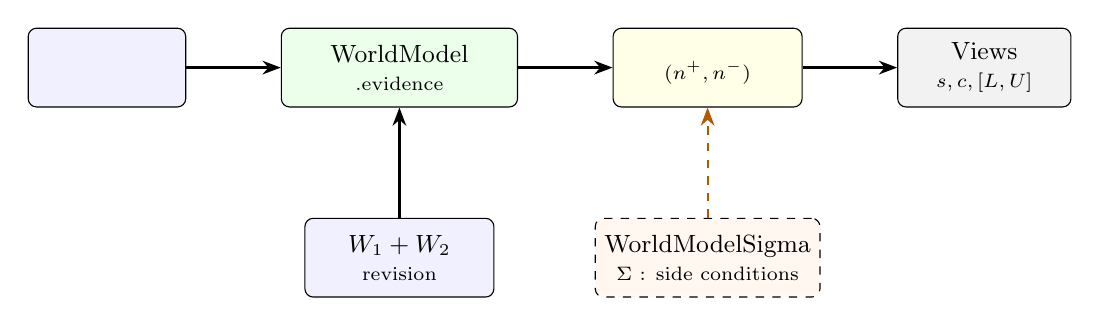
\begin{tikzpicture}[
  >=Stealth,
  every node/.style={font=\small},
  box/.style={draw, rounded corners=3pt, align=center,
              minimum height=10mm},
]
\node[box, fill=blue!6, minimum width=20mm] (q) {\PLNQuery{}};
\node[box, fill=green!8, minimum width=30mm, right=12mm of q] (wm)
  {\code{WorldModel}\\[-1pt]{\scriptsize\code{.evidence}}};
\node[box, fill=yellow!10, minimum width=24mm, right=12mm of wm] (ev)
  {\Evidence{}\\[-1pt]{\scriptsize$(n^+, n^-)$}};
\node[box, fill=gray!10, minimum width=22mm, right=12mm of ev] (view)
  {Views\\[-1pt]{\scriptsize$s, c, [L,U]$}};

\draw[->, thick] (q) -- (wm);
\draw[->, thick] (wm) -- (ev);
\draw[->, thick] (ev) -- (view);

% revision loop beneath
\node[box, fill=blue!6, minimum width=24mm, below=14mm of wm] (rev)
  {$W_1 + W_2$\\[-1pt]{\scriptsize revision}};
\draw[->, thick] (rev) -- (wm);

% sigma bundle
\node[draw, dashed, rounded corners=3pt, fill=orange!6,
      minimum width=28mm, minimum height=10mm,
      below=14mm of ev, align=center] (sig)
  {\code{WorldModelSigma}\\[-1pt]{\scriptsize$\Sigma$ : side conditions}};
\draw[->, dashed, thick, orange!70!black] (sig) -- (ev);
\end{tikzpicture}
\caption{The world-model query interface.  A \PLNQuery{} is answered by
extracting \Evidence{} from the world-model state; views are lossy
projections.  Revision ($+$) combines states.  A \code{WorldModelSigma}
bundles structural side conditions for compiled rewrites.}
\label{fig:query-worldmodel-flow}
\end{figure}

\section{World Models with Side Conditions}

For compiled inference, we often need structural assumptions about the world
model: a DAG structure for a Bayesian network, conditional independence
conditions, positivity hypotheses.  We capture this with a
\emph{sigma-bundled world model}:

\begin{lstlisting}
structure WorldModelSigma (State : Type*) (Query : Type*)
    [EvidenceType State] where
  wm : WorldModel State Query
  sigma : Prop  -- side-condition context
\end{lstlisting}

The $\Sigma$ (side-condition context) is a proposition that the world model
satisfies additional structural properties.  Every compiled rewrite carries
its $\Sigma$ explicitly---there are no hidden assumptions.

\section{The Solomonoff Connection}

The \nuPLN{} framework of Nil Geisweiller~\cite{nuPLN2026} grounds PLN in
Solomonoff Universal Induction.  The key ideas fold naturally into the
world-model framework:

The \emph{global probability space} $(\Omega, \mathcal{F}, \nu)$
corresponds to a world-model state where $\Omega$ is the set of possible
worlds, each containing a probabilistic predicate
$\hat{\mu} : \mathcal{D} \to \Omega \to \mathrm{Bool}$ and its complete
evaluation history.  The \emph{universal distribution} $\nu$ then defines
a prior over possible generators $\hat{\mu} \in \mathcal{L}$, where
$\mathcal{L}$ is a probabilistic programming language; Bayesian updating
with observed evidence produces the posterior.  The \emph{observable
predicate}~$\mu$---the true generator---lives in the true world~$\omega$,
and an observer has access only to a finite subset of evaluations, which
is precisely the evidence.  Finally, concepts and predicates are isomorphic
via satisfying sets and indicator functions: the inheritance relationship
$A \Rightarrow B$ on the concept side corresponds to implication on the
predicate side.  We work on the predicate side throughout.

The crucial insight from \nuPLN{} is that de~Finetti's representation
theorem~\cite{definetti1937} justifies evidence counts as sufficient
statistics.  For an infinite exchangeable sequence of binary observations,
the counts $(n^+, n^-)$ contain all the information needed for Bayesian
updating.  When we assume a Beta prior $\text{Beta}(\alpha, \beta)$, the
posterior after observing $n^+$ positive and $n^-$ negative outcomes is
$\text{Beta}(\alpha + n^+, \beta + n^-)$.

This is why PLN's evidence representation $(n^+, n^-)$ is not merely a
convenient bookkeeping device---it is the \emph{sufficient statistic} for
the posterior under the exchangeability assumption.  Chapter~\ref{ch:evidence}
develops this algebraic structure in detail.


\chapter{Reference Complete Semantics: Posterior-State Calculus}
\label{ch:posterior-state}

\begin{quote}\small
\textbf{Goal:} Define the core calculus: posterior revision + query interface.\\
\textbf{Semantic object:} Dirichlet posterior state over worlds; revision and conditioning.\\
\textbf{Proved:} Revision commutation; deduction formula admissibility; sequent rules.\\
\textbf{Assumed:} Finite propositional scope (atoms indexed by $\mathrm{Fin}(n)$).
\end{quote}

The complete core calculus is intentionally simple.  It is the calculus of
revising posterior states plus a query interface.  Everything else in
\xiPLN{}---evidence algebras, truth-value views, compiled rules, tractable
fragments---is built on top of this core.

\begin{figure}[htbp]
\centering
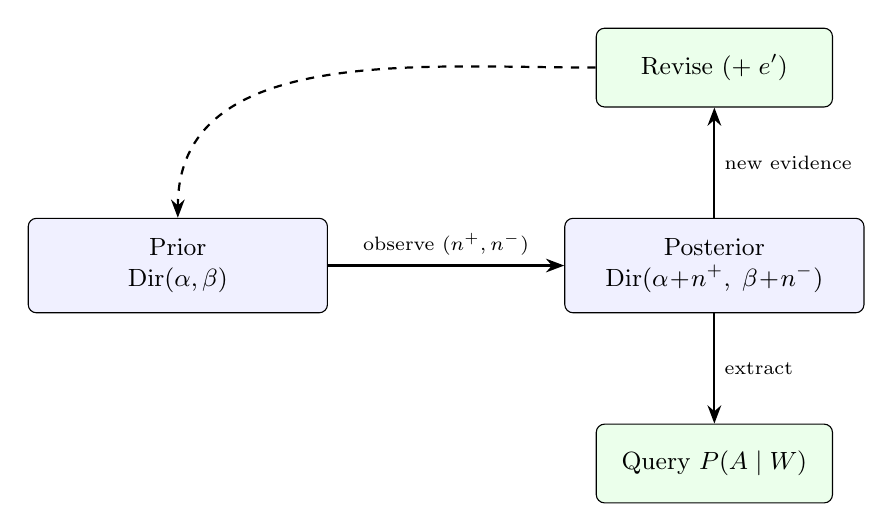
\begin{tikzpicture}[
  >=Stealth,
  every node/.style={font=\small},
  box/.style={draw, rounded corners=3pt, fill=blue!6, align=center,
              minimum width=38mm, minimum height=12mm},
  op/.style={draw, rounded corners=3pt, fill=green!8, align=center,
             minimum width=30mm, minimum height=10mm},
]
\node[box] (prior) {Prior\\$\mathrm{Dir}(\alpha,\beta)$};
\node[box, right=30mm of prior] (post)
  {Posterior\\$\mathrm{Dir}(\alpha\!+\!n^+,\;\beta\!+\!n^-)$};
\node[op, below=14mm of post] (query) {Query $P(A \mid W)$};
\node[op, above=14mm of post] (revise) {Revise $(+\;e')$};

\draw[->, thick] (prior) -- node[above, font=\scriptsize] {observe $(n^+, n^-)$} (post);
\draw[->, thick] (post) -- node[right, font=\scriptsize] {extract} (query);
\draw[->, thick] (post) -- node[right, font=\scriptsize] {new evidence} (revise);
\draw[->, thick, dashed] (revise.west) to[out=180, in=90] (prior.north);
\end{tikzpicture}
\caption{The posterior-state update cycle.  A Dirichlet prior is updated by
observing evidence counts, producing a posterior.  The posterior answers
queries (downward) and accepts further revision (upward, cycling back).}
\label{fig:posterior-update-cycle}
\end{figure}

\section{The Reference Instance: Dirichlet over Worlds}

For finite propositional scope (atoms indexed by $\mathrm{Fin}(n)$), we
instantiate the \WorldModel{} interface with a Dirichlet world-table:
\[
  \JointEvidence(n) := \mathrm{Fin}(2^n) \to \mathbb{R}_{\ge 0}^{\infty}
\]
interpreted as Dirichlet pseudo-counts over the $2^n$ complete worlds.
Each coordinate $E(w)$ records how much evidence supports world $w$.

Evidence extraction works by summation over the worlds compatible with
each query type.  For a propositional query $\code{prop}(A)$, the
extractor sums counts where atom~$A$ is true (positive evidence) versus
false (negative evidence).  For a link query $\code{link}(A, B)$, it sums
counts where $A$ is true and $B$ is true against those where $A$ is true
and $B$ is false---conditioning on the antecedent.  For a conditional-link
query $\code{linkCond}([A_1, \ldots, A_k], B)$, it sums counts where all
$A_i$ hold and $B$ holds versus all $A_i$ hold and $B$ fails, giving the
multi-parent conditional evidence that Bayesian-network CPTs require.

Revision is pointwise addition of pseudo-counts.  The Lean prototype proves
that this satisfies the world-model interface, including the critical
compositionality law:
\[
  \mathrm{ev}(E_1 + E_2, q) = \mathrm{ev}(E_1, q) \hplus \mathrm{ev}(E_2, q)
\]
for all queries $q$.

See \codepath{Mettapedia/Logic/PLNJointEvidence.lean}.

\section{The Sequent-Calculus View}

We present \xiPLN{} as a sequent-style system with two contexts:
\begin{itemize}
\item An \emph{evidence context} $\Gamma$, a finite multiset of posterior
  fragments (elements of the state type).
\item A \emph{side-condition context} $\Sigma$, containing structural
  assumptions about the chosen world-model class (e.g., a BN DAG,
  positivity, d-separation facts).
\end{itemize}

\subsection{Judgments}

Two judgment forms suffice:
\begin{enumerate}
\item \textbf{World-model judgment:}
  $\Sigma; \Gamma \vdash_{\mathrm{wm}} W$---from the evidence pieces in
  $\Gamma$, we construct the revised posterior state $W$.

\item \textbf{Query judgment:}
  $\Sigma; \Gamma \vdash q \Downarrow e$---querying the revised posterior
  derived from $\Gamma$ yields evidence $e$ for query $q$.
\end{enumerate}

When \code{State} is an additive commutative monoid, the world-model
judgment is deterministic: $W := \sum \Gamma$.  The query judgment then
extracts via the world-model interface: $e := \mathrm{ev}(W, q)$.

\subsection{Core Rules}

The complete core calculus consists of four rules:
\[
\frac{}{\Sigma; \varnothing \vdash_{\mathrm{wm}} 0}
\;(\text{WM-Unit})
\qquad
\frac{}{\Sigma; \{W\} \vdash_{\mathrm{wm}} W}
\;(\text{WM-Ev})
\]
\[
\frac{\Sigma; \Gamma \vdash_{\mathrm{wm}} W \quad
      \Sigma; \Delta \vdash_{\mathrm{wm}} W'}
     {\Sigma; \Gamma \uplus \Delta \vdash_{\mathrm{wm}} (W + W')}
\;(\text{WM-Rev})
\]
\[
\frac{\Sigma; \Gamma \vdash_{\mathrm{wm}} W}
     {\Sigma; \Gamma \vdash q \Downarrow \mathrm{ev}(W, q)}
\;(\text{Q-Extract})
\]

The key algebraic law---evidence compositionality---makes the following
\emph{query-revision} rule admissible:
\[
\frac{\Sigma; \Gamma \vdash q \Downarrow e \quad
      \Sigma; \Delta \vdash q \Downarrow e'}
     {\Sigma; \Gamma \uplus \Delta \vdash q \Downarrow (e \hplus e')}
\;(\text{Q-Rev})
\]

\paragraph{Links are queries.}
In this view, a PLN ``link'' $A \Rightarrow B$ is not an object-level
connective; it is a query \code{link(A, B)} against the revised world model.
The calculus does not propagate links directly; it revises world models and
answers link queries.

\section{Probability Views}

From \Evidence{} we obtain posterior-mean probabilities:
\[
  P(A) = \frac{\#(A)}{\#(\top)}, \qquad
  P(B \mid A) = \frac{\#(A \wedge B)}{\#(A)}
\]
where $\#(\cdot)$ denotes world-count sums in \JointEvidence{}.  The Lean
file \codepath{Mettapedia/Logic/PLNJointEvidenceProbability.lean} proves
the exact ratio forms for these views.

\section{Derived Link Calculus: Classic PLN Rules as Admissible Rewrites}

Classic PLN rules become \emph{admissible query rewrites} relative to a
world-model class with explicit side conditions $\Sigma$.

\subsection{The Deduction Formula}

The PLN deduction rule computes $P(C \mid A)$ by total probability:
\begin{align}
  P(C \mid A) &= P(C \mid A, B)\,P(B \mid A) + P(C \mid A, \lnot B)\,P(\lnot B \mid A)
  \label{eq:total-prob}
\end{align}

Under the \emph{screening-off} conditions
$P(C \mid A, B) = P(C \mid B)$ and
$P(C \mid A, \lnot B) = P(C \mid \lnot B)$, this simplifies to:
\begin{align}
  P(C \mid A) &= P(C \mid B)\,P(B \mid A)
    + P(C \mid \lnot B)\,(1 - P(B \mid A))
  \label{eq:deduction-screened}
\end{align}

Writing $s_{AB} = P(B \mid A)$, $s_{BC} = P(C \mid B)$, $s_B = P(B)$,
$s_C = P(C)$, and eliminating $P(C \mid \lnot B)$ via
$s_C = s_B \cdot s_{BC} + (1 - s_B) \cdot P(C \mid \lnot B)$, we obtain:

\begin{definition}[PLN deduction strength]
\label{def:deduction-strength}
\[
  \mathrm{plnDed}(s_{AB}, s_{BC}, s_B, s_C) \;:=\;
  s_{AB} \cdot s_{BC} + (1 - s_{AB}) \cdot \frac{s_C - s_B \cdot s_{BC}}{1 - s_B}
\]
defined when $0 < s_B < 1$.
\end{definition}

\begin{theorem}[Chain BN deduction exactness (\claimConditional{})]
\label{thm:chain-deduction}
Let $W$ be a chain BN world model $A \to B \to C$.  Under the explicit
hypotheses:
\begin{enumerate}
\item[(i)] $0 < \strength(W, \code{prop}(B)) < 1$ \quad (positivity),
\item[(ii)] $\Sigma \vdash C \perp\!\!\!\perp A \mid B$ and
  $C \perp\!\!\!\perp A \mid \lnot B$ \quad (screening-off),
\end{enumerate}
we have:
\[
  \strength(W, \code{link}(A, C)) = \mathrm{plnDed}\big(
    \strength(W, \code{link}(A, B)),\;
    \strength(W, \code{link}(B, C)),\;
    \strength(W, \code{prop}(B)),\;
    \strength(W, \code{prop}(C))
  \big).
\]
\end{theorem}

In Lean:
\begin{lstlisting}
theorem chainBN_plnDeductionStrength_exact
    (hpos : 0 < queryStrength W (PLNQuery.prop B))
    (hlt  : queryStrength W (PLNQuery.prop B) < 1)
    (hso  : screeningOff W A B C) :
    queryStrength W (PLNQuery.link A C) =
    plnDeductionStrength
      (queryStrength W (PLNQuery.link A B))
      (queryStrength W (PLNQuery.link B C))
      (queryStrength W (PLNQuery.prop B))
      (queryStrength W (PLNQuery.prop C))
\end{lstlisting}

The analogous result holds for fork BNs $A \leftarrow B \to C$
(\code{forkBN\_plnDeductionStrength\_exact}).

See \codepath{Mettapedia/Logic/PLNBayesNetFastRules.lean}.

\subsection{Induction and Abduction}

Induction and abduction arise from the same total-probability structure
but with different known/unknown roles:

\begin{itemize}
\item \textbf{Induction:} given $P(A \mid B)$ and $P(A \mid C)$,
  estimate $P(C \mid B)$.  This inverts the direction of the conditional.
\item \textbf{Abduction:} given $P(B \mid A)$ and $P(B \mid C)$,
  estimate $P(A \mid C)$.  This inverts the conditioning.
\end{itemize}

Both require their own screening-off conditions, which are
formally stated in the Lean proofs.

See \codepath{Mettapedia/Logic/PLNDerivation.lean}.


\chapter{The Local-Completeness No-Go Theorem}
\label{ch:no-go}

\begin{quote}\small
\textbf{Goal:} Establish the fundamental limit of local link-level inference.\\
\textbf{Semantic object:} World tables with distinct marginal-compatible joint structures.\\
\textbf{Proved:} No-go: complete link evidence cannot be computed from per-link evidence alone.\\
\textbf{Assumed:} Nothing (unconditional counterexample).
\end{quote}

One might hope for a system that takes local per-link evidence
($\Evidence$ for $A$, $B$, $C$, $A \Rightarrow B$, $B \Rightarrow C$)
and computes complete evidence for $A \Rightarrow C$.  \xiPLN{} asserts
that this is impossible in general.

\boundarystart
\begin{theorem}[No local complete deduction rule (\claimBoundary{})]
\label{thm:no-go}
There is no function
\[
  f : \Evidence^5 \to \Evidence
\]
that, for all joint evidence states $E$, computes the exact link evidence
for $A \Rightarrow C$ from only the local premises
$\mathrm{ev}(E, A)$, $\mathrm{ev}(E, B)$, $\mathrm{ev}(E, C)$,
$\mathrm{ev}(E, A \Rightarrow B)$, $\mathrm{ev}(E, B \Rightarrow C)$.
\end{theorem}
\boundaryend

\begin{proof}[Proof sketch]
For three atoms $A, B, C$, there are $2^3 = 8$ possible worlds.
We construct two joint evidence states $E_1, E_2 :
\mathrm{Fin}(8) \to \mathbb{R}_{\ge 0}$ that agree on all five
marginal evidence values:
\[
  \mathrm{ev}(E_1, A) = \mathrm{ev}(E_2, A), \quad
  \mathrm{ev}(E_1, B) = \mathrm{ev}(E_2, B), \quad
  \mathrm{ev}(E_1, C) = \mathrm{ev}(E_2, C),
\]
\[
  \mathrm{ev}(E_1, A \!\Rightarrow\! B) = \mathrm{ev}(E_2, A \!\Rightarrow\! B), \quad
  \mathrm{ev}(E_1, B \!\Rightarrow\! C) = \mathrm{ev}(E_2, B \!\Rightarrow\! C),
\]
but disagree on the conclusion:
\[
  \mathrm{ev}(E_1, A \!\Rightarrow\! C) \ne \mathrm{ev}(E_2, A \!\Rightarrow\! C).
\]

The key: world entries corresponding to $(A\!=\!1, B\!=\!0, C\!=\!1)$
and $(A\!=\!1, B\!=\!1, C\!=\!0)$ can be traded off against each other
while preserving all five marginals.  But this trade changes the
$A \Rightarrow C$ evidence because it redistributes mass among worlds
where $A$ is true.

Since the five marginals cannot distinguish $E_1$ from $E_2$, no
function $f : \Evidence^5 \to \Evidence$ can compute $\mathrm{ev}(E, A \!\Rightarrow\! C)$
correctly for both states.
\end{proof}

See \codepath{Mettapedia/Logic/PLNJointEvidenceNoGo.lean}.

\begin{figure}[htbp]
\centering
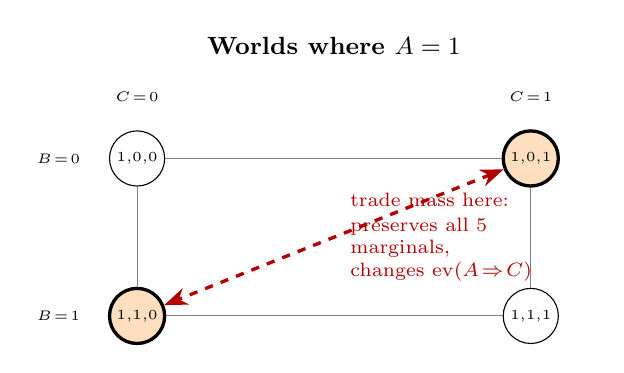
\begin{tikzpicture}[
  >=Stealth,
  every node/.style={font=\scriptsize},
  world/.style={draw, circle, minimum size=7mm, inner sep=1pt},
  swap/.style={draw, circle, minimum size=7mm, inner sep=1pt,
               fill=orange!25, very thick},
]
% A=1 slice (the critical part)
\node[font=\small\bfseries, anchor=south] at (2.5, 3.2) {Worlds where $A=1$};

\node[world] (w100) at (0, 2) {$\scriptscriptstyle 1,0,0$};
\node[swap]  (w101) at (5, 2) {$\scriptscriptstyle 1,0,1$};
\node[swap]  (w110) at (0, 0) {$\scriptscriptstyle 1,1,0$};
\node[world] (w111) at (5, 0) {$\scriptscriptstyle 1,1,1$};

% grid lines
\draw[thin, gray] (w100) -- (w101);
\draw[thin, gray] (w100) -- (w110);
\draw[thin, gray] (w101) -- (w111);
\draw[thin, gray] (w110) -- (w111);

% swap arrow
\draw[<->, very thick, red!70!black, dashed]
  (w101) -- node[right=2pt, font=\scriptsize, text width=30mm, align=left]
  {trade mass here:\\[1pt] preserves all 5 marginals,\\changes $\mathrm{ev}(A\!\Rightarrow\! C)$}
  (w110);

% axis labels
\node[font=\tiny, anchor=east] at (-0.6, 2) {$B\!=\!0$};
\node[font=\tiny, anchor=east] at (-0.6, 0) {$B\!=\!1$};
\node[font=\tiny, anchor=south] at (0, 2.6) {$C\!=\!0$};
\node[font=\tiny, anchor=south] at (5, 2.6) {$C\!=\!1$};
\end{tikzpicture}
\caption{The no-go witness.  Among the four worlds where $A\!=\!1$,
redistributing mass between $(1,0,1)$ and $(1,1,0)$ (orange) preserves
all five local marginals ($A$, $B$, $C$, $A\!\Rightarrow\! B$,
$B\!\Rightarrow\! C$) but changes $\mathrm{ev}(A\!\Rightarrow\! C)$.
No function of the five marginals can detect this trade.}
\label{fig:no-go-witness}
\end{figure}

\section{Interpretation}

This theorem is the formal core of ``you must carry correlations.''
It does \emph{not} make fast PLN useless.  It tells us exactly what fast
PLN \emph{cannot} claim: completeness for arbitrary world models without
structural assumptions.

The constructive response is to:
\begin{enumerate}
\item \textbf{Restrict the model class.}  For Bayesian networks with
  explicit DAG structure, the factorization makes local computation
  exact (Chapter~\ref{ch:bn-models}).
\item \textbf{State the assumptions.}  Every compiled rule carries its
  $\Sigma$ context, so the user knows exactly when the fast rule applies.
\item \textbf{Provide corrected alternatives.}  Where an original PLN
  formula required an unstated assumption, provide the corrected
  side-conditioned version alongside the boundary theorem.
\end{enumerate}


%% ═══════════════════════════════════════════════════════════════════
\part{Evidence and Truth-Value Views}
\label{part:evidence}
%% ═══════════════════════════════════════════════════════════════════

\chapter{Evidence Algebra}
\label{ch:evidence}

\begin{quote}\small
\textbf{Goal:} Develop the algebraic structure of observation-count evidence.\\
\textbf{Semantic object:} \Evidence{} with revision ($\hplus$), ordering, quantale ($\htensor$), Heyting lattice.\\
\textbf{Proved:} Quantale and Heyting frame axioms; information ordering is a lattice.\\
\textbf{Assumed:} Nothing.
\end{quote}

Evidence is the currency of PLN.  Before any inference rule fires, before
any truth value is computed, evidence must be collected, combined, and
compared.  This chapter develops the algebraic structure of evidence.

\section{Evidence as Counts}

The basic evidence type in PLN is a pair of non-negative counts:
\[
  \Evidence := (n^+, n^-) \in \mathbb{N} \times \mathbb{N}
\]
where $n^+$ counts positive observations and $n^-$ counts negative
observations.  (In the Lean formalization, we sometimes work over
$\mathbb{R}_{\ge 0}$ or $\mathbb{R}_{\ge 0}^\infty$ for compatibility
with measure-theoretic constructions.)

The total sample size is $n = n^+ + n^-$.  The \emph{strength} view
(posterior mean) is $s = n^+ / n$ when $n > 0$.  But we must resist
the temptation to conflate the evidence $(n^+, n^-)$ with its
strength view $s$---evidence carries strictly more information.

See \codepath{Mettapedia/Logic/EvidenceClass.lean}.

\section{Revision as Addition}

The fundamental operation on evidence is \emph{revision}: combining two
bodies of evidence into one.  Revision is componentwise addition:
\[
  (n_1^+, n_1^-) \hplus (n_2^+, n_2^-) = (n_1^+ + n_2^+, n_1^- + n_2^-)
\]
This is associative, commutative, and has unit $(0, 0)$---the evidence
of having observed nothing.

The justification for additive revision comes from de~Finetti's
representation theorem.  For exchangeable binary sequences, the counts
are sufficient statistics for the posterior.  Adding counts corresponds to
Bayesian conjugate updating with a Beta prior:
\[
  \text{Beta}(\alpha + n_1^+, \beta + n_1^-)
  \;\;\xrightarrow{+\;(n_2^+, n_2^-)}\;\;
  \text{Beta}(\alpha + n_1^+ + n_2^+, \beta + n_1^- + n_2^-)
\]

This is why evidence revision is \emph{addition}: it is the algebraic
shadow of Bayesian conjugate updating.

\section{Information Ordering}

Evidence values are partially ordered by information content:
\[
  (n_1^+, n_1^-) \le (n_2^+, n_2^-) \iff
  n_1^+ \le n_2^+ \;\wedge\; n_1^- \le n_2^-
\]
More evidence is always at least as informative.  This ordering makes
$\Evidence$ a lattice with meet (componentwise min) and join (componentwise
max).

\section{Quantale Structure}

Beyond the additive monoid and lattice, $\Evidence$ carries a
\emph{quantale} structure.  A quantale is a complete lattice equipped
with a monoidal operation $\htensor$ that distributes over arbitrary
joins:
\[
  a \htensor \Big(\bigvee_{i \in I} b_i\Big) = \bigvee_{i \in I} (a \htensor b_i)
\]

For $\Evidence = (n^+, n^-)$, the tensor is defined as:
\[
  (a^+, a^-) \htensor (b^+, b^-) = (a^+ \cdot b^+,\; a^+ \cdot b^- + a^- \cdot b^+)
\]
with unit $(1, 0)$.  This corresponds to the compositional combination of
dependent evidence streams: observing $a$ and then observing $b$ conditional
on $a$ being positive.

\begin{theorem}[Quantale transitivity (\claimCore{})]
\label{thm:quantale-trans}
For evidence values $e_{AB}$, $e_{BC}$ representing
$A \Rightarrow B$ and $B \Rightarrow C$ respectively:
\[
  e_{AB} \htensor e_{BC} \;\le\; e_{AC}
\]
in the information ordering.  Equality holds under the screening-off
conditions.
\end{theorem}

This inequality is the algebraic shadow of the deduction rule:
the tensor product of premise evidence provides a lower bound on the
conclusion evidence.

See \codepath{Mettapedia/Logic/EvidenceQuantale.lean}.

\section{Heyting Structure}

$\Evidence$ also forms a Heyting algebra with an explicit
pseudo-complement:

\begin{definition}[Heyting implication on $\Evidence$ (\claimCore{})]
The relative pseudo-complement is defined componentwise:
\[
  (a^+, a^-) \Rightarrow (b^+, b^-) =
  \Big(\,\begin{cases} \top & \text{if } a^+ \le b^+ \\
                        b^+ & \text{otherwise}\end{cases},\;\;
        \begin{cases} \top & \text{if } a^- \le b^- \\
                        b^- & \text{otherwise}\end{cases}\,\Big)
\]
satisfying the residuation law:
$a \le b \Rightarrow c \iff a \wedge b \le c$.
\end{definition}

The Heyting complement (negation) is $\neg a = a \Rightarrow \bot = a \Rightarrow (0,0)$.

This is important because the evidence algebra supports \emph{intuitionistic}
logical operations.  In particular, the law of excluded middle fails:
$a \vee \neg a \ne \top$ in general, because there may be no evidence at all.

A key formalized fact---the ``totality gate''---establishes that
$\Evidence$ has incomparable elements (e.g., $(3, 0)$ and $(0, 3)$) and
admits no faithful order-embedding into the reals.  No single real-valued
function captures all evidence information.

See \codepath{Mettapedia/Logic/HeytingValuationOnEvidence.lean} and
\codepath{Mettapedia/Logic/PLN\_KS\_Bridge.lean}.

\begin{figure}[htbp]
\centering
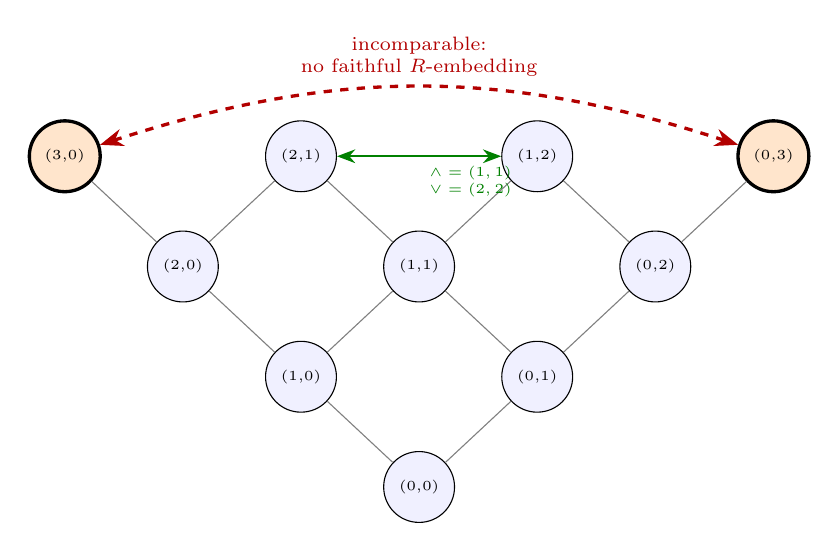
\begin{tikzpicture}[
  >=Stealth,
  every node/.style={font=\scriptsize},
  ev/.style={draw, circle, minimum size=9mm, inner sep=1pt, fill=blue!6},
  inc/.style={draw, circle, minimum size=9mm, inner sep=1pt, fill=orange!20,
              very thick},
]
% Row 0
\node[ev] (00) at (3, 0) {$\scriptscriptstyle(0,0)$};
% Row 1
\node[ev] (10) at (1.5, 1.4) {$\scriptscriptstyle(1,0)$};
\node[ev] (01) at (4.5, 1.4) {$\scriptscriptstyle(0,1)$};
% Row 2
\node[ev] (20) at (0, 2.8) {$\scriptscriptstyle(2,0)$};
\node[ev] (11) at (3, 2.8) {$\scriptscriptstyle(1,1)$};
\node[ev] (02) at (6, 2.8) {$\scriptscriptstyle(0,2)$};
% Row 3
\node[inc] (30) at (-1.5, 4.2) {$\scriptscriptstyle(3,0)$};
\node[ev] (21) at (1.5, 4.2) {$\scriptscriptstyle(2,1)$};
\node[ev] (12) at (4.5, 4.2) {$\scriptscriptstyle(1,2)$};
\node[inc] (03) at (7.5, 4.2) {$\scriptscriptstyle(0,3)$};

% Hasse edges
\draw[thin, gray] (00) -- (10);
\draw[thin, gray] (00) -- (01);
\draw[thin, gray] (10) -- (20);
\draw[thin, gray] (10) -- (11);
\draw[thin, gray] (01) -- (11);
\draw[thin, gray] (01) -- (02);
\draw[thin, gray] (20) -- (30);
\draw[thin, gray] (20) -- (21);
\draw[thin, gray] (11) -- (21);
\draw[thin, gray] (11) -- (12);
\draw[thin, gray] (02) -- (12);
\draw[thin, gray] (02) -- (03);

% incomparable highlight
\draw[<->, very thick, red!70!black, dashed]
  (30) to[bend left=18]
  node[above, font=\scriptsize, text width=32mm, align=center]
    {incomparable:\\no faithful $\mathbb{R}$-embedding}
  (03);

% meet/join annotation
\draw[<->, thick, green!50!black] (21) --
  node[below right, font=\tiny, text width=22mm, align=left]
    {$\wedge = (1,1)$\\$\vee = (2,2)$}
  (12);
\end{tikzpicture}
\caption{Hasse diagram of the \Evidence{} lattice (first four levels).
The information ordering is componentwise: $(a^+, a^-) \le (b^+, b^-)$
iff both coordinates are $\le$.  Orange nodes $(3,0)$ and $(0,3)$ are
incomparable---no single real-valued function preserves the full ordering
(the ``totality gate'').  The green link shows meet and join:
$\wedge\!\big((2,1),(1,2)\big) = (1,1)$, $\vee = (2,2)$.}
\label{fig:evidence-lattice}
\end{figure}

\section{What Evidence Algebra Is Not}

Evidence algebra is \emph{not} the complete probabilistic semantics.
It is a compositional bookkeeping layer.  The world-model posterior
(Chapter~\ref{ch:posterior-state}) carries strictly more information
than the extracted per-query evidence values.  The no-go theorem
(Chapter~\ref{ch:no-go}) makes this precise: per-link evidence cannot
reconstruct the joint state.

Evidence algebra is to probability theory what bookkeeping is to
economics: indispensable for accounting, but not a substitute for the
underlying model of the economy.


\chapter{Truth-Value Views: Strength, Confidence, Intervals}
\label{ch:tv-views}

\begin{quote}\small
\textbf{Goal:} Define strength, confidence, and interval bounds as lossy projections of evidence.\\
\textbf{Semantic object:} View functions from \Evidence{} to $\mathbb{R}$ or $[\ell, u]$.\\
\textbf{Proved:} View monotonicity; Walley/Kyburg interval reduction; views are not proof objects.\\
\textbf{Assumed:} Nothing.
\end{quote}

Operationally, PLN works with compact summaries of evidence:
a strength, a confidence, sometimes an interval.  These are \emph{views}---
projections from the evidence algebra into simpler spaces that are useful
for thresholding, display, and approximate computation.

\begin{figure}[htbp]
\centering
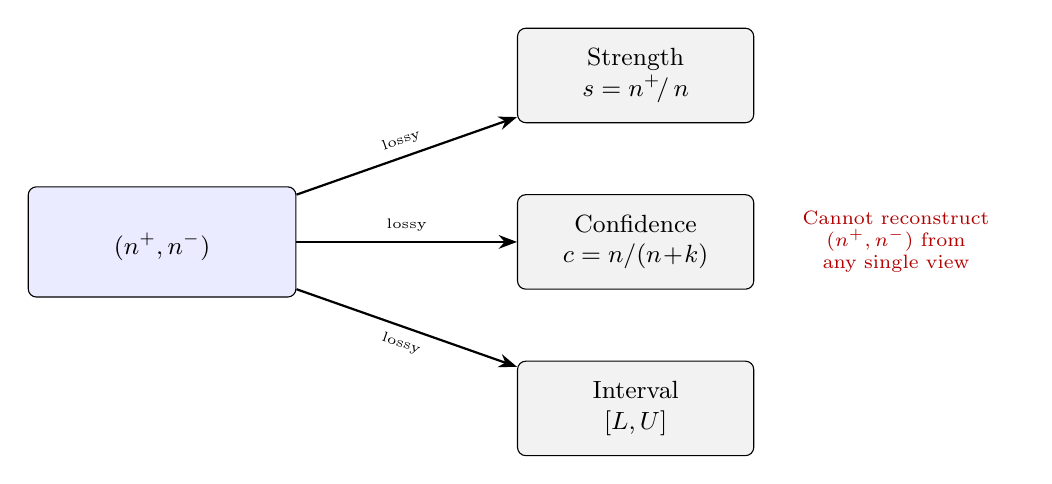
\begin{tikzpicture}[
  >=Stealth,
  every node/.style={font=\small},
  src/.style={draw, rounded corners=3pt, fill=blue!8, align=center,
              minimum width=34mm, minimum height=14mm},
  tgt/.style={draw, rounded corners=3pt, fill=gray!10, align=center,
              minimum width=30mm, minimum height=12mm},
]
\node[src] (ev) {\Evidence{}\\$(n^+, n^-)$};
\node[tgt, above right=8mm and 28mm of ev] (str)
  {Strength\\$s = n^+\!/\,n$};
\node[tgt, right=28mm of ev] (conf)
  {Confidence\\$c = n/(n\!+\!k)$};
\node[tgt, below right=8mm and 28mm of ev] (itv)
  {Interval\\$[L, U]$};

\draw[->, thick] (ev) -- node[above, font=\tiny, sloped] {lossy} (str);
\draw[->, thick] (ev) -- node[above, font=\tiny] {lossy} (conf);
\draw[->, thick] (ev) -- node[below, font=\tiny, sloped] {lossy} (itv);

% no-reconstruct annotation
\node[font=\scriptsize, text width=30mm, align=center, red!70!black]
  at ($(conf.east) + (18mm, 0)$)
  {Cannot reconstruct\\$(n^+, n^-)$ from\\any single view};
\end{tikzpicture}
\caption{Truth-value views are lossy projections from \Evidence{}.
Strength, confidence, and interval bounds each discard information.
No single view suffices to reconstruct the original evidence counts.}
\label{fig:tv-views-projections}
\end{figure}

\section{Simple Truth Values}

A \emph{simple truth value} (STV) is a pair $\STV{s}{c}$ where:
\begin{itemize}
\item $s = n^+ / (n^+ + n^-)$ is the \emph{strength}---the posterior mean
  under a uniform prior, or equivalently the maximum-likelihood estimate
  of the underlying probability.
\item $c = n / (n + k)$ is the \emph{confidence}---a monotone function of
  the total sample size $n = n^+ + n^-$, parameterized by a lookahead
  $k > 0$.  Confidence ranges from $0$ (no evidence) to approaching $1$
  (overwhelming evidence).
\end{itemize}

The STV is the most commonly used truth-value representation in PLN
practice.  It is compact and intuitive.  But it is a \emph{lossy} view:
two different evidence values can produce the same STV (when they have
the same ratio $n^+/n$ and the same total $n$), and the STV discards
information about the shape of the posterior distribution beyond its
mean.

\section{Confidence as a View}

Confidence deserves special attention.  In the original PLN presentation,
confidence often appears as a standalone quantity that can be manipulated
independently of strength.  In \xiPLN{}, confidence is strictly a derived
view:
\[
  \confidence(n^+, n^-) = \frac{n^+ + n^-}{n^+ + n^- + k}
\]

The parameter $k$ controls how much evidence is needed before the system
becomes ``confident.''  For $k = 1$, a single observation gives
confidence $0.5$; for $k = 10$, ten observations give confidence
$0.5$.

The key property: confidence is monotone in the total evidence count.
More evidence always means higher (or equal) confidence.

\section{Indefinite Truth Values}

An \emph{indefinite truth value} (ITV) provides interval bounds on the
strength:
\[
  \mathrm{ITV} = [s_L,\; s_U,\; b,\; w]
\]
where $s_L$ and $s_U$ are lower and upper bounds, $b$ is a confidence-like
parameter, and $w = s_U - s_L$ is the interval width.

There are at least three distinct semantic interpretations of such
intervals, and they \emph{must not be conflated}:

\begin{enumerate}
\item \textbf{Bayesian credible intervals.}  An interval
  $[s_L, s_U]$ such that the posterior probability
  $\Pr(s_L \le p \le s_U \mid \text{data})$ exceeds some threshold.
  These depend on the prior.

\item \textbf{Walley-style predictive intervals (IDM).}  Intervals
  derived from the Imprecise Dirichlet Model~\cite{Walley1991,Walley1996BagOfMarbles},
  which provide robust predictions without committing to a single prior.
  These are prior-free but give wider intervals.

\item \textbf{Frequentist confidence intervals.}  Intervals constructed
  so that the true parameter lies within them with specified coverage
  probability over repeated sampling.
\end{enumerate}

The original PLN book sometimes uses the notation $[L, U]$ without
specifying which semantics is intended.  \xiPLN{} insists on explicit
selector choice: the user declares which interval semantics they want,
and the system computes accordingly.

See \codepath{Mettapedia/Logic/PLNIndefiniteTruth.lean} and
\codepath{Mettapedia/Logic/PLNWorldModelITV.lean}.

\section{Why Views Are Not Proof Objects}

Views are useful.  They are indispensable for practical inference.  But
they are \emph{not} the right objects to pass between inference steps.
The reason: views are lossy projections.  When you chain two inferences
using only the STV of the intermediate result, you have already lost
information about the shape of the posterior, the correlation structure,
and the raw evidence counts.

The \xiPLN{} discipline is: carry evidence (or world-model states)
between inference steps; extract views only at the end, for display
or decision-making.  The slogan again:

\begin{quote}
\emph{Probability is what you query; evidence is what you carry.}
\end{quote}


\chapter{Distributional and Interval Semantics}
\label{ch:distributional}

\begin{quote}\small
\textbf{Goal:} Develop the distributional layer: Beta, Dirichlet, and Normal-Gamma posteriors.\\
\textbf{Semantic object:} Conjugate posterior families as evidence carriers.\\
\textbf{Proved:} Conjugate update laws; sleep consolidation; distributional dominance over scalar; convergence.\\
\textbf{Assumed:} Conjugate-family restriction (posteriors stay in the same family).
\end{quote}

Beyond point estimates and intervals, PLN supports a richer
\emph{distributional} layer where the truth value is an entire
posterior distribution over possible probability values.

\section{Beta Distributions and Evidence}

For a single binary predicate observed $n^+$ times true and $n^-$ times
false, the posterior under a Beta prior $\text{Beta}(\alpha, \beta)$ is:
\[
  p \mid \text{data} \;\sim\; \text{Beta}(\alpha + n^+, \beta + n^-)
\]

Evidence counts $(n^+, n^-)$ are the natural parameters of this
posterior.  Revision (adding counts) corresponds to Bayesian conjugate
updating.  The posterior mean is
\[
  \mathbb{E}[p] = \frac{\alpha + n^+}{\alpha + \beta + n^+ + n^-}
\]
which, for a uniform prior ($\alpha = \beta = 1$), gives the strength
\[
  s = \frac{1 + n^+}{2 + n^+ + n^-}
\]
This is the Laplace-smoothed estimate.

See \codepath{Mettapedia/Logic/EvidenceBeta.lean}.

\section{Dirichlet Distributions for Multi-Valued Domains}

For predicates with more than two outcomes, the Beta generalizes to the
Dirichlet distribution.  Evidence becomes a vector of counts, and
conjugate updating extends componentwise.

See \codepath{Mettapedia/Logic/EvidenceDirichlet.lean}.

\section{Normal-Gamma Evidence for Continuous Domains}
\label{sec:normal-gamma}

The Beta and Dirichlet families handle discrete observations.  For
continuous observations---sensor readings, measurements, real-valued
features---the appropriate conjugate family is the
\emph{Normal-Gamma}~\cite{BernardoSmith2000}.

For observations $x_1, \ldots, x_n \sim \mathcal{N}(\mu, 1/\tau)$
with unknown mean~$\mu$ and precision~$\tau$, the evidence is the
sufficient statistic $(n, \textstyle\sum x_i, \sum x_i^2)$.  The prior
is $\text{Normal-Gamma}(\mu_0, \kappa_0, \alpha_0, \beta_0)$ and the
posterior is Normal-Gamma with updated parameters:
\[
  \kappa_n = \kappa_0 + n, \qquad
  \mu_n = \frac{\kappa_0 \mu_0 + \sum x_i}{\kappa_n}, \qquad
  \alpha_n = \alpha_0 + \tfrac{n}{2}
\]
\[
  \beta_n = \beta_0
    + \tfrac{1}{2}\bigl(\textstyle\sum x_i^2 - (\sum x_i)^2/n\bigr)
    + \frac{\kappa_0 \, n \, (\bar{x} - \mu_0)^2}{2\kappa_n}
\]

Revision is again componentwise addition of sufficient statistics:
\[
  (n_1, s_1, q_1) \hplus (n_2, s_2, q_2) = (n_1 + n_2,\; s_1 + s_2,\; q_1 + q_2)
\]
and the key compositionality theorem is:
\begin{theorem}[Sleep Consolidation (\claimCore{})]
\label{thm:sleep-consolidation}
  $\text{posterior}(\pi, e_1 \hplus e_2)
   = \text{posterior}(\text{posterior}(\pi, e_1), e_2)$
  for any prior~$\pi$ and realizable evidence $e_1, e_2$.
\end{theorem}
This states that batch replay of deferred observations yields the same
posterior as sequential Bayesian updating---the mathematical foundation
for ``sleep as evidence consolidation.''

The confidence analog carries over directly: $c = n/(n + \kappa)$,
the same formula as binary PLN.  The pattern is uniform across all
conjugate families:

\medskip
\begin{center}
\begin{tabular}{lll}
  \textbf{Domain} & \textbf{Evidence} & \textbf{Prior family} \\
  \hline
  Binary  & $(n^+, n^-)$ & Beta$(\alpha, \beta)$ \\
  Categorical & count vector & Dirichlet$(\boldsymbol\alpha)$ \\
  Continuous  & $(n, \sum x_i, \sum x_i^2)$ & Normal-Gamma$(\mu_0, \kappa_0, \alpha_0, \beta_0)$
\end{tabular}
\end{center}
\medskip

See \codepath{Mettapedia/Logic/EvidenceNormalGamma.lean}.

\paragraph{Two-layer architecture.}
\label{sec:two-layer}
Each demo below has two layers.
\emph{Lean} proves the posterior formulas correct and establishes
structural properties (consolidation, independence, monotonicity),
all kernel-checked.  A companion Python script
(\texttt{scripts/wm\_pln\_posterior.py}) instantiates the proved
formulas on each fixture to produce concrete numerical results:
posterior means, 95\% credible intervals, exceedance probabilities,
and classification scores.  The Student-$t$ predictive CDF fills the
role of the abstract \texttt{ExceedanceSpec} that Lean leaves parametric
(Mathlib lacks a Normal CDF).  We also compare with scikit-learn's
\texttt{GaussianNB}; the two agree on clearly separated regimes
(e.g.\ K\_Scratch at $x=3.6$) but differ at ambiguous boundary
points (e.g.\ $x=2.0$), since GaussianNB uses ML point estimates
while the Normal-Gamma posterior predictive integrates over parameter
uncertainty.  The added value of the WM-PLN formulation is:
(a)~the Lean proofs guarantee formula correctness,
(b)~the framework generalizes to hybrid discrete/continuous states, and
(c)~sleep consolidation is \emph{proved}, not assumed.
\paragraph{Data hygiene.}
The demos below use small, traceable fixture slices
(5--15 data points per class) drawn from real datasets---not
full benchmark-scale evaluations.  Their purpose is to serve as
\emph{theorem-backed empirical canaries} that exercise the proved formulas
on genuine data; larger-scale validation on the full Steel dataset
appears in Section~\ref{sec:steel-full}.  Throughout:
(i)~fitting uses only training data;
(ii)~``sleep consolidation'' steps use only previously observed evidence,
never future labels;
(iii)~the \emph{promotion boundary} between canary fixtures and
full-dataset validations is always marked explicitly.

\paragraph{PLN-to-WM concept mapping.}
\label{sec:pln-wm-map}
Table~\ref{tab:pln-wm-map} shows how each core PLN concept maps to
its WM-PLN formalization.  The left column uses the terminology of
the PLN book~\cite{goertzel2009pln}; the right column gives the Lean
module or theorem that formalizes the concept.

\begin{table}[ht]
\centering
\caption{PLN concept $\to$ WM-PLN formalization.}
\label{tab:pln-wm-map}
\begin{tabular}{@{}lllp{3.8cm}@{}}
\toprule
\textbf{PLN Concept} & \textbf{PLN Book} & \textbf{WM-PLN} & \textbf{Lean Reference} \\
\midrule
Evidence count
  & $(n^+,\, n^-)$
  & $(n,\;\Sigma x_i,\;\Sigma x_i^2)$
  & \code{EvidenceNormalGamma} \\[3pt]
Strength
  & $s = \frac{n^+}{n^+ + n^-}$
  & Posterior mean $\mu_n$
  & \code{posterior\_mu\_eq\_of\_realizable} \\[3pt]
Confidence
  & $c = \frac{n}{n + k}$
  & $c = \frac{n}{n + \kappa_0}$ (monotone)
  & \code{confidence\_monotone} \\[3pt]
Revision ($\oplus$)
  & Componentwise add
  & \code{hplus} on suff.\ stats
  & \code{NormalGammaEvidence.hplus} \\[3pt]
Sleep consolidation
  & ---
  & $\pi(e_1 \oplus e_2) = \pi(\pi(e_1), e_2)$
  & \code{posterior\_hplus\_of\_realizable} \\[3pt]
Exceedance query
  & ---
  & $P(X_{\mathrm{new}} > c)$
  & \code{ExceedanceSpec} \\[3pt]
Source attribution
  & Implicit
  & Explicit source counts
  & \code{PLNWidgetFactoryDemo} \\[3pt]
De~Finetti
  & Informal
  & Finite exchangeable model
  & \code{DeFinetti.lean} \\
\bottomrule
\end{tabular}
\end{table}

\paragraph{Measure-theoretic grounding.}
\label{sec:measure-ground}
The Normal-Gamma family is a joint prior \emph{measure} on
$(\mu, \tau) \in \mathbb{R} \times \mathbb{R}_+$, where $\tau = 1/\sigma^2$
is the precision.  The posterior update proved in
\code{EvidenceNormalGamma.lean} is the algebraic form of Bayes'
theorem applied to this measure: given $n$ observations $x_1, \ldots, x_n$
drawn from $\mathcal{N}(\mu, \tau^{-1})$, the likelihood factors through
the sufficient statistics $(n, \sum x_i, \sum x_i^2)$ by the
Fisher--Neyman factorization theorem.  Conjugacy ensures the posterior
remains Normal-Gamma, so the update reduces to arithmetic on the four
hyperparameters $(\mu_0, \kappa_0, \alpha_0, \beta_0)$.

The Lean formalization proves this arithmetic \emph{exactly}: the
closed-form expressions for $\mu_n$, $\kappa_n$, $\alpha_n$, $\beta_n$
are established in \code{posterior\_mu\_eq\_of\_realizable} and
\code{posterior\_beta\_eq\_of\_realizable}, and per-demo bridge theorems instantiate them on each demo's
concrete fixture data.  The integral form of the posterior (involving the
Gamma density $\mathrm{Ga}(\alpha_0, \beta_0)$) is standard
mathematics~\cite{BernardoSmith2000} (Ch.~5); Mathlib provides
\code{gaussianPDFReal} and Lebesgue integration, but the Gamma
density is not yet available in Mathlib, so the integral derivation
is not formalized today.

\paragraph{Experiment-family view.}
The Gaussian suite is a family of \emph{experiment types}, not a single
benchmark leaderboard.  Each study exercises a different aspect of the
world-model calculus:
the Gas Sensor study tests \emph{drift governance and replay semantics};
the GJP forecasting study tests \emph{source-reliability weighting and
recalibration under temporal forgetting}.
Steel serves as a \emph{same-model-class validation}---does the
formalized conjugate classifier improve on the plain GaussianNB baseline,
and can its posterior confidence drive principled abstention?
NAB is an \emph{honest boundary case}: it exercises a real scoring
pipeline with verified Kalman updates, but it is not presented as a
full-corpus leaderboard result.
This division is deliberate.  The distinctive contribution of a
world-model approach is not raw tabular accuracy but queryable
uncertainty, replay semantics, soft evidence, and explicit reasoning
about which experiment channel is more informative.

\paragraph{Comparator taxonomy.}
To keep the empirical claims honest, the manuscript uses three
\emph{different kinds of comparator}, and they should not be conflated.
\begin{enumerate}
\item \textbf{WM-PLN models.} These are the evidence/world-model systems
formalized in Lean and evaluated in the main applied chapters.
\item \textbf{Proper probabilistic-programming baselines.} When the book
refers to \emph{Stan} in the PPLBench appendix, it means the standard
PPLBench Stan backend under \codepath{pplbench/ppls/stan/}, not an
ad hoc one-off script.  The same family includes PyMC, JAGS, NumPyro,
and BeanMachine where available.  Appendix~\ref{app:pplbench-stan-pln}
now includes a direct \codepath{normal\_normal} Stan $\leftrightarrow$
WM-PLN run on that proper PPLBench surface.
\item \textbf{External statistical/ML baselines.} \texttt{GaussianNB},
\texttt{XGBoost}, and Windowed Gaussian are not WM-PLN variants; they are
separate classical baselines used to show where WM-style semantics help,
where they do not, and when WM is acting as a governance/support layer
rather than a replacement predictor.
\end{enumerate}

\begin{table}[htbp]
\centering
\footnotesize
\setlength{\tabcolsep}{4pt}
\renewcommand{\arraystretch}{0.96}
\caption{Comparator families used in the empirical sections.}
\label{tab:comparator-taxonomy}
\begin{tabular}{p{2.6cm}p{3.0cm}p{7.8cm}}
\toprule
Family & Representative tools & Meaning in this book \\
\midrule
WM-PLN &
Lean-backed evidence/world-models &
Primary object of study: typed evidence accumulation, replay, confidence,
forgetting, and governance semantics. \\
\addlinespace
Proper PPL baselines &
Stan, PyMC, JAGS, NumPyro, BeanMachine &
Used to compare against mainstream probabilistic inference systems on
shared benchmark models in PPLBench.  ``Stan'' refers to the standard
PPLBench Stan backend, not a scratch prototype. \\
\addlinespace
Classical statistical / ML baselines &
\texttt{GaussianNB}, \texttt{XGBoost}, Windowed Gaussian &
Used in the applied studies to distinguish same-model-class wins
(\texttt{GaussianNB}), stronger discriminative baselines
(\texttt{XGBoost}), and standard anomaly controls (Windowed Gaussian). \\
\bottomrule
\end{tabular}
\end{table}

\begin{table}[htbp]
\centering
\footnotesize
\setlength{\tabcolsep}{4pt}
\renewcommand{\arraystretch}{0.96}
\caption{Role split across the current real-data study slices.  The empirical
  spine has two co-flagships (Gas and GJP), one supporting validation
  (Steel), and one honest negative boundary (NAB).}
\label{tab:dataset-role-split}
\begin{tabular}{p{2.4cm}p{3.2cm}p{3.2cm}p{5.4cm}}
\toprule
Dataset & WM-PLN role & Key metric & Main finding \\
\midrule
Steel (3-class, 27 feat.) &
supporting same-model-class validation / abstention &
AURC &
WM-PLN beats GaussianNB (0.0346 vs 0.1061) but not XGBoost (0.0126), so the selective-prediction win is strongest within the conjugate Bayesian model class. \\
\addlinespace
Gas (3-gas, 128 feat.) &
co-flagship: drift trigger / replay governance &
sample-weighted accuracy under label budget &
Frozen XGBoost gives 67.9\%; a cheap confidence trigger reaches 79.9\% with one retrain and 18.8\% labels. \\
\addlinespace
Gas (6-gas, 128 feat.) &
co-flagship: drift trigger / replay governance &
sample-weighted accuracy under label budget &
Frozen XGBoost gives 46.7\%; XGBoost confidence is the best cheap trigger (64.5\% at 23.9\% labels) while WM/XGBoost agreement is the strongest high-accuracy trigger (67.0\% at 86.8\% labels). \\
\addlinespace
GJP forecasting &
co-flagship: source reliability / recalibration &
Brier, log score, AURC, sleep invariance &
WM reliability weighting improves over stronger top-k log/logit pooling baselines on year-4 Brier/log and selective AURC while matching accuracy; a WM-agreement gate still improves the strong top-$k$ pool on the multi-option slice; nightly batch consolidation matches online updates to machine precision, and forgetting early years improves year-4 calibration. \\
\addlinespace
NAB &
negative boundary / case study &
official corpus raw score &
The current 1D Kalman residual detector is not competitive on the full corpus ($-116.0$ vs.\ Windowed Gaussian $-24.0$), so NAB remains a narrow protocol-semantics case study. \\
\bottomrule
\end{tabular}
\end{table}

\subsection{Applied Example: Hybrid Sensor Monitoring}

The \emph{broken sensor demo} exercises continuous world models end-to-end.
A sensor monitoring system combines:
\begin{itemize}
\item \textbf{Continuous temperature evidence} modeled by Normal-Gamma
  sufficient statistics (5~normal readings, 5~elevated readings).
\item \textbf{Boolean cooling-failure evidence} modeled by binary counts
  (2~failures in 100~checks).
\end{itemize}
The hybrid state is a product type; revision operates componentwise.
Queries are answered by extracting binary \Evidence{} from each component:
cooling failure is read directly; temperature exceedance $P(X > c)$ is
handled via an abstract \emph{exceedance specification}---a function
satisfying monotonicity properties---since Mathlib lacks a Normal CDF.

Key results (all kernel-checked):
\begin{enumerate}
\item Sleep consolidation (Theorem~\ref{thm:sleep-consolidation}):
  morning + night batch = sequential update.
\item Confidence monotonicity: more observations $\Rightarrow$ higher
  $c = n/(n + \kappa)$.
\item Exceedance ordering: $P(X > c_\text{crit}) \le P(X > c_\text{warn})$
  for $c_\text{crit} > c_\text{warn}$.
\item Independence: temperature and cooling-failure evidence components
  do not interfere.
\end{enumerate}

\begin{figure}[htbp]
\centering
\includegraphics[width=0.85\textwidth]{../results/figures/broken_sensor.pdf}
\caption{Broken sensor demo: prior predictive (gray dashed), posterior
  after morning shift (blue, concentrated around 16\textdegree{}C),
  after night shift (red, shifted to 22\textdegree{}C), and
  consolidated posterior (green dashed, between the two).
  Data tick marks on the $x$-axis.}
\label{fig:broken-sensor}
\end{figure}

\paragraph{Numerical results.}
With prior $\mathrm{NG}(15, 1, 2, 10)$, the morning shift
(5 readings, mean 15.92) yields posterior $\mu_n = 15.77$,
95\% CI $[11.96, 19.57]$, $P(X > 20) = 0.017$, confidence $c = 0.83$.
The night shift (5~readings, mean 22.72) yields $\mu_n = 21.43$,
$P(X > 20) = 0.674$---night readings strongly indicate an overheated
state.  Sleep consolidation is verified numerically: sequential update
through morning then night produces the same posterior
($\mu_n = 18.93$) as batch processing all 10 readings at once.

See \codepath{Mettapedia/Logic/PLNBrokenSensorDemo.lean} (420 lines).

\subsection{Applied Example: Widget Factory Source-Conditional Mixtures}

The \emph{widget factory demo} extends the continuous story to
\textbf{multiple sources with per-source Gaussian evidence}.
A factory has two machines (A,~B); each widget arrives with an observed
source label and a real-valued feature measurement.  Each machine has
its own Normal-Gamma prior and evidence accumulates per-source.

The genuinely new theorems are the \textbf{mixture exceedance} results:
\begin{enumerate}
\item \emph{Mixture validity.}  For weights $w_A + w_B = 1$
  ($w_i \ge 0$) and per-source exceedance probabilities
  $p_A, p_B \in [0,1]$, the mixture
  $p_{\mathrm{mix}} = w_A p_A + w_B p_B$ satisfies
  $0 \le p_{\mathrm{mix}} \le 1$.

\item \emph{Mixture bounds.}  $\min(p_A, p_B) \le p_{\mathrm{mix}}
  \le \max(p_A, p_B)$---the mixture lies between its components.
\end{enumerate}
Additional results: per-machine sleep consolidation, source
independence (machine~A observations do not affect machine~B's
posterior), confidence monotonicity, and source weight normalization.

\paragraph{Numerical results.}
Machine~A (prior $\mu_0 = 10$, 4~readings, mean 9.90): posterior
$\mu_n = 9.92$, 95\% CI $[7.05, 12.79]$, $P(X > 12) = 0.067$.
Machine~B (prior $\mu_0 = 10.5$, 3~readings, mean 11.10): posterior
$\mu_n = 10.95$, 95\% CI $[7.71, 14.19]$, $P(X > 12) = 0.234$.
Machine~B is about $3.5\times$ more likely to produce a defect
($>$12) than Machine~A, consistent with its higher operating mean.

See \codepath{Mettapedia/Logic/PLNWidgetFactoryDemo.lean} (422 lines).

\subsection{Applied Example: Kalman Filter Wake/Sleep Temporal Filtering}

The \emph{Kalman sleep demo} adds \textbf{temporal dynamics} to the
continuous story.  A~1D position is tracked via a random-walk process
model ($x_{t+1} = x_t + w_t$, $w_t \sim N(0,\sigma_w^2)$) observed
through a noisy sensor ($z_t = x_t + v_t$, $v_t \sim N(0,\sigma_v^2)$).

\paragraph{Core operations.}
\begin{itemize}
\item \emph{Predict}: variance inflates by $\sigma_w^2$ (mean unchanged).
\item \emph{Update}: Kalman gain $K = \sigma^2/(\sigma^2 + \sigma_v^2)$
  shifts the mean toward the measurement and shrinks the variance by
  the factor $(1-K)$.
\item \emph{Step} = predict then update.
\end{itemize}

\paragraph{Key formal results (all kernel-checked).}
\begin{enumerate}
\item \emph{Kalman gain bounded:} $0 < K < 1$ and $1-K = \sigma_v^2/(\sigma^2+\sigma_v^2)$.
\item \emph{Variance reduction:} each measurement strictly reduces
  uncertainty: $(1-K)\sigma^2 < \sigma^2$.
\item \emph{Closed-form updated variance:}
  $\sigma^2_{\mathrm{new}} = \sigma^2 \sigma_v^2 / (\sigma^2 + \sigma_v^2)$.
\item \emph{Sleep $=$ Wake} (the flagship theorem):
  \[
    \mathsf{filterOrbit}(b_0,\; \mathit{morning} \mathbin{+\!+} \mathit{night})
    \;=\;
    \mathsf{filterOrbit}\bigl(\mathsf{filterOrbit}(b_0,\;\mathit{morning}),\;
      \mathit{night}\bigr)
  \]
  via \texttt{List.foldl\_append}---batch replay of deferred
  observations yields the \emph{same} posterior as sequential online
  filtering.  A three-shift generalization is also proved.
\item \emph{Exceedance threshold ordering:}
  $P(\text{pos} > c_{\mathrm{crit}}) \le P(\text{pos} > c_{\mathrm{warn}})$
  whenever $c_{\mathrm{warn}} \le c_{\mathrm{crit}}$.
\end{enumerate}

\paragraph{Wake/sleep narrative.}
The \emph{wake} phase is online Kalman filtering: measurements arrive
one-by-one and each predict-update cycle refines the belief.  The
\emph{sleep} phase replays a batch of deferred observations---and
the central theorem guarantees the result is identical.  This gives a
formal grounding for ``sleep consolidation'' in the PLN activation
framework: batch replay is semantically equivalent to real-time
processing, not an approximation.

\paragraph{Numerical results.}
Initial Kalman gain $K_0 = 0.913$ (high, reflecting large prior
uncertainty $\sigma^2_0 = 10$).  After morning (5~readings, mean 1.94):
posterior mean $= 1.96$, $\sigma^2 = 0.50$.  After night
(5~more, mean 3.10): posterior mean $= 3.14$, $\sigma^2 = 0.50$.
Sleep $=$ wake is verified to machine precision: batch replay of all
10 readings from the initial state produces the same posterior as
sequential morning-then-night processing.

See \codepath{Mettapedia/Logic/PLNKalmanSleepDemo.lean} (374 lines).

\subsection{Applied Example: Gas Sensor Array Drift Classification}

The \emph{gas sensor drift demo} is one of the chapter's two empirical
\textbf{co-flagships}: the main \textbf{drift/replay governance} study
in the Gaussian suite.  It brings \textbf{real-world data} into the
Gaussian demo suite.  The UCI Gas Sensor Array Drift
Dataset~\cite{Vergara2012GasSensorDrift} (DOI~10.24432/C5RP6W)
contains 13,910 measurements from 16 chemical sensors exposed to
6~gas types over 36~months (10~batches, January~2007 to
February~2011).  Vergara et~al.\ achieve 80--95\% gas classification
accuracy using SVM ensembles on all 128~features with drift
compensation.  Our Lean demo still focuses on a single-sensor fixture
for theorem proving, but the surrounding numerical layer now also runs
full 128-feature drift protocols so that the same WM-PLN update laws can
be compared against standard classification baselines.

\paragraph{Setup.}
We extract a small fixture: sensor~1 steady-state resistance ($\Delta R$)
for three target gases---\emph{ethanol}, \emph{ammonia}, and
\emph{toluene}---with 5 samples per gas from batch~1 (early calibration)
and batch~10 (late drift epoch).  Each gas type has its own
Normal-Gamma prior; the state tracks ternary source-attribution counts.

\paragraph{Illustrative CANARY fixture.}
This 5-sample single-sensor fixture is an \textbf{illustrative CANARY}
for the proved Gaussian sleep/independence laws.  The headline empirical
claims in this section come from the full 128-feature drift protocols
and governance policies below, not from the hand-picked fixture.

\paragraph{Key formal results (all kernel-checked).}
\begin{enumerate}
\item \emph{Per-gas sleep consolidation:} for each gas type,
  $\mathrm{posterior}(\pi, e_1 \oplus e_2)
    = \mathrm{posterior}(\mathrm{posterior}(\pi, e_1), e_2)$.
  Batch replay $=$ sequential update.
\item \emph{Cross-gas independence:} ethanol observations produce
  zero evidence in the ammonia and toluene posteriors, and vice versa
  (6 independence theorems).
\item \emph{Multi-batch composition:} batch~1 $+$ batch~10 $=$
  full dataset, with associativity across gas sub-batches.
\item \emph{3-way source weight normalization:}
  $n_E/(n_E{+}n_A{+}n_T) + n_A/(n_E{+}n_A{+}n_T) + n_T/(n_E{+}n_A{+}n_T) = 1$.
\item \emph{Confidence monotonicity} and \emph{exceedance anti-threshold}
  generalize from the earlier demos.
\end{enumerate}

\paragraph{Drift narrative.}
Batch~1 toluene responses are high ($\sim$138k $\Delta R$) while batch~10
responses are dramatically lower ($\sim$24k), reflecting genuine sensor
degradation over 36~months.  The Normal-Gamma posteriors from each epoch
capture this shift: the posterior mean for toluene moves substantially
between batches.  Sleep consolidation still holds across drifted epochs---
the mathematical guarantee is that deferred assimilation preserves the
posterior, regardless of whether the underlying distribution has shifted.
Detecting \emph{whether} drift occurred requires comparing posteriors
from different epochs, which the framework supports but does not automate.

\begin{figure}[htbp]
\centering
\includegraphics[width=\textwidth]{../results/figures/gas_sensor_drift.pdf}
\caption{Gas sensor array drift.  Solid curves: batch~1 posterior
  predictive (2007).  Dashed: consolidated posterior after both
  batches.  Toluene shows dramatic drift: batch~10 responses (crosses)
  cluster near zero, far from the batch~1 distribution.}
\label{fig:gas-sensor-drift}
\end{figure}

\begin{figure}[htbp]
\centering
\includegraphics[width=\textwidth]{../results/figures/gas_drift_protocols.pdf}
\caption{Gas sensor drift protocols on the full 128-feature representation.
  Cumulative replay is the strongest average protocol in both the 3-gas and
  6-gas settings.  Iterative unlabeled replay / E-M is scientifically useful
  precisely because it is mixed: recent-batch seeding improves over batch-1
  seeding on average, but unlabeled adaptation still remains below cumulative
  labeled replay and can become unstable on the hardest late batch.}
\label{fig:gas-drift-protocols}
\end{figure}

\paragraph{Numerical results.}
After batch~1 (5~readings each): ethanol posterior mean $37{,}270$,
95\% CI $[7{,}601,\, 66{,}939]$; ammonia $7{,}079$,
CI $[2{,}672,\, 11{,}486]$; toluene $137{,}655$,
CI $[89{,}711,\, 185{,}598]$.
Exceedance $P(X > 50{,}000)$: ethanol $0.179$, ammonia $<0.001$,
toluene $0.999$---the WM-PLN framework correctly identifies toluene
as the gas producing strong sensor responses.
After consolidating both batches (10~readings), toluene's posterior mean
drops to $81{,}565$ with a wide CI reflecting the dramatic drift
($\Delta = -114{,}055$ between epochs).  Confidence for each gas
rises from $c = 0.980$ (5~readings) to $c = 0.990$ (10~readings).

\paragraph{Full-dataset drift study.}
We extend the fixture demo to the full 128-feature representation under
the standard drift protocols used in the gas-sensor
literature~\cite{Jiang2021BDA}.  On the 3-gas subset
(ethanol/ammonia/toluene), an independent-feature WM-PLN classifier
reaches 68.4\% under ``Setting~1'' (train batch~1, test batches~2--10),
72.1\% under ``Setting~2'' (train batch~$k{-}1$, test batch~$k$), and
73.6\% under cumulative \emph{sleep replay} (train batches~1\ldots$k{-}1$,
test batch~$k$); the GaussianNB baselines are 68.2\%, 75.8\%, and 71.2\%.
On the full 6-gas task the numbers are 47.3\%/53.0\%/53.2\% (WM-PLN)
versus 47.3\%/51.2\%/52.5\% (GaussianNB).

These figures are substantially below domain-adaptation methods---Balanced
Distribution Adaptation reports 68.92\% (Setting~1) and 81.06\%
(Setting~2) on the same benchmark~\cite{Jiang2021BDA}.  The point is not
to compete with specialized drift-compensation algorithms, but to exhibit
the qualitative effect of the world-model calculus: late-batch drift
degrades accuracy, and replaying additional batches into the posterior
partially recovers it \emph{without changing the underlying update laws}.
The replay is a consequence of the evidence algebra, not a separate
engineering mechanism.

\paragraph{Soft replay / E-M adaptation.}
Naive unlabeled adaptation is brittle under strong multi-class drift, and
this matters more than the positive cases.  The weighted Gaussian E/M
extension provides a \emph{soft-evidence adaptation} protocol: batch~1
anchors the source posterior, unlabeled target data drives an E-step over
responsibilities, and the M-step revises each class posterior by weighted
sufficient statistics.  On the 3-gas task, iterative soft replay
($\lambda=0.2$, mean 5.4~iterations) reaches 67.8\% on average---below
cumulative labeled replay's 73.5\%---but still improves the hardest
batch~10 from 63.6\% to 73.3\%.  Seeding from the most recent labeled
batch instead of batch~1 raises the average to 70.7\%, but collapses to
37.3\% on batch~10 because the recent seed is itself small and
unrepresentative.  On the full 6-gas task, batch~1-seeded adaptation
drops to 42.0\%, recent-batch seeding recovers to 50.4\%, and both
remain below labeled replay's 53.3\%.

The lesson: soft evidence helps when the current posterior is stale, but
unlabeled adaptation should be treated as a policy component---to be
invoked selectively---not as a drop-in replacement for labeled replay.
This is exactly the kind of replay-policy question the world-model
experiment layer is designed to express.

\begin{figure}[htbp]
\centering
\includegraphics[width=\textwidth]{../results/figures/gas_xgboost_wm_support.pdf}
\caption{Gas drift support for a stronger base learner.  The relevant question
  is not whether WM-PLN replaces XGBoost, but whether WM-derived agreement
  signals can support abstention and replay decisions under drift.
  Calibrated XGBoost confidence (sigmoid or isotonic) does not improve
  the risk--coverage curve in this setting, while WM/XGBoost agreement
  remains the most interesting selective signal on the harder 6-gas task.}
\label{fig:gas-xgboost-support}
\end{figure}

\paragraph{Supporting stronger tabular models.}
The world-model calculus is not a replacement for strong discriminative
classifiers; it is a governance layer that supplies a second epistemic
signal for abstention and retraining decisions.  The gas benchmark is the
right place to test this framing.  Training XGBoost on batch~1 alone gives 67.9\% average
accuracy on the 3-gas task and 46.7\% on the 6-gas task.  If we use the
batch~1 WM posterior only as a confidence score, the result is worse:
plain WM confidence is not a good wrapper here.  The more interesting
signal is \emph{agreement} between XGBoost and the source WM posterior.
We also compared against calibrated XGBoost confidence, since a machine
learning reviewer might reasonably ask whether ordinary post-hoc
probability calibration already solves the abstention problem.  In this
drifted gas setting it does not: sigmoid calibration worsens AURC from
0.1374 to 0.2114 on the 3-gas task and from 0.3847 to 0.3994 on the
6-gas task, while isotonic calibration degrades further to 0.2135 and
0.4639.  So the interesting comparison is not ``native versus calibrated
XGBoost,'' but ``XGBoost's own confidence versus a second epistemic
signal supplied by the WM.''  On the harder 6-gas task,
agreement-gated selective prediction improves
the area under the risk--coverage curve from 0.3847 (native XGBoost
confidence) to 0.3737, and the agreement subset itself covers 59.7\% of
samples at 59.7\% accuracy, versus 46.7\% overall.  On the 3-gas task,
agreement gating is not a blanket win (AURC 0.1483 vs.\ 0.1374 for
native XGBoost), but it still isolates a 74.8\% coverage subset at
75.3\% accuracy.

The batch-level support story is stronger still once we treat drift as a
\emph{sequential policy problem}.  We stream batches~2\ldots10 in order,
retain the batch~1 XGBoost model as the default predictor, and decide at
each batch whether to acquire labels and replay all previously seen
batches into a refreshed model.  This turns WM-PLN into a
\emph{governance layer}: it does not replace XGBoost, but supplies a
second epistemic signal that can trigger abstention or retraining.

\begin{lstlisting}[caption={Gas drift governance protocol (shipped confidence/agreement triggers; no lookahead into batch-$k$ labels).},label={lst:gas-governance-protocol}]
Initialize labeled_batches = {1}.
Train XGBoost and WM on labeled_batches only.

for batch k = 2..10:
    freeze the current models before any batch-k labels are used
    predict batch k with the frozen XGBoost model
    compute xgboost_confidence_mean(batch k)
    compute wm_confidence_mean(batch k)
    compute wm_agreement_coverage(batch k)
    decide acquire_labels_k from these shipped model-derived statistics only

    record batch-k accuracy for the frozen model
    if acquire_labels_k:
        request labels for batch k
        add batch k to the labeled replay buffer
        retrain on all labeled batches seen so far
        use the refreshed models only for future batches
    else:
        keep the current models unchanged

Report sample-weighted accuracy, retrain_events,
and label_budget_fraction.
\end{lstlisting}

The resulting frontier is informative rather than trivial.  On the
3-gas task, a simple XGBoost-confidence trigger at 0.80 is the best
low-cost policy we tested: it raises sample-weighted accuracy from
67.9\% to 79.9\% with only one retraining event and a 18.8\% label
budget.  A more aggressive WM-agreement trigger at 0.80 reaches a
similar 79.1\% accuracy, but requires five retraining events and a
53.4\% label budget.  On the harder 6-gas task, the tradeoff is more
interesting: XGBoost-confidence gating at 0.80 reaches 64.5\% accuracy
with four retrains and 23.9\% labels, while WM-agreement gating at 0.80
pushes raw accuracy slightly higher to 67.0\% but consumes 86.8\% of the
labels and seven retraining events.  The utility sweep therefore has two
regimes: XGBoost confidence is the best \emph{cheap} trigger, while
WM/XGBoost agreement is the best \emph{accuracy-seeking} trigger when
label cost is low.  That is exactly the support role we want from
WM-PLN: not ``beating XGBoost'' as another tabular learner, but
governing when a stronger learner should be trusted, deferred, or
replayed.

\begin{table}[htbp]
\centering
\caption{Gas drift as a governance problem rather than a raw benchmark.
  AURC compares selective prediction signals; the policy columns summarize
  the strongest sequential retraining results at fixed label budgets.}
\label{tab:gas-governance-summary}
\begin{tabular}{lcccccc}
\toprule
Task & Native & Sigmoid & Isotonic & WM agree &
Best $\le 25\%$ labels & Best raw accuracy \\
\midrule
3-gas &
0.1374 &
0.2114 &
0.2135 &
0.1483 &
79.9\% @ 18.8\% &
79.9\% @ 18.8\% \\
6-gas &
0.3847 &
0.3994 &
0.4639 &
0.3737 &
64.5\% @ 23.9\% &
67.0\% @ 86.8\% \\
\bottomrule
\end{tabular}
\end{table}

\begin{figure}[htbp]
\centering
\includegraphics[width=\textwidth]{../results/figures/gas_policy_frontier.pdf}
\caption{Sequential gas-drift support policies.  Each point is a batch-level
  retraining policy over batches~2\ldots10, trading sample-weighted
  accuracy against label budget.  XGBoost confidence is the best cheap
  trigger, while WM/XGBoost agreement is the strongest high-accuracy
  trigger when labels are inexpensive.}
\label{fig:gas-policy-frontier}
\end{figure}

The order-cost layer now formalizes this governance story directly:
\code{gasScheduleErrorCount\_batchSwap\_eq\_zero},
\code{gasRuntimePairwiseOrderCheck\_batchSwap\_zero}, and
\code{gasOrderBudgetPolicy\_batchSwap\_zero\_via\_runtimeCertificate}
show that a zero-threshold policy is certifiably safe for additive
batch-swap composition in this lane.
The module also exposes gas-specific zero-threshold endpoints for
ethanol, ammonia, and toluene.
See \codepath{Mettapedia/Logic/PLNWorldModelOrderCostGasPolicyDemo.lean}.

See \codepath{Mettapedia/Logic/PLNGasSensorDriftDemo.lean} (652~lines).

\subsection{Applied Example: Steel Plates Fault Classification}

The \emph{steel plates fault demo} is a \textbf{supporting same-model-class
validation}, not a headline benchmark.  It applies the
source-conditional Gaussian pattern to \textbf{manufacturing quality
control}.  The UCI
Steel Plates Faults Dataset~\cite{Buscema2010SteelPlates}
(current UCI DOI~10.24432/C5J88N) contains 1,941 instances with 27 features
and 7 fault classes.  Published results using all 27~features report
$\sim$73.6\% (SVM), $\sim$79.5\% (Random Forest), and 86.655\%
(LMT Forest) 7-class accuracy~\cite{Ghasemkhani2023LMTForest}.  Our
core Lean model uses a single feature
(LogOfAreas), so lower accuracy is expected and the purpose is
formal correctness, not SOTA competition.

\paragraph{Setup.}
We extract a small fixture: LogOfAreas measurements for three fault
types---\emph{Pastry} (pop.\ mean~$\approx 2.4$, $\sigma \approx 0.48$),
\emph{K\_Scratch} (pop.\ mean~$\approx 3.6$, $\sigma \approx 0.70$),
and \emph{Bumps} (pop.\ mean~$\approx 2.1$, $\sigma \approx 0.36$)---with
5 samples per class.  For K\_Scratch, we select samples at the 10th--90th
percentiles to represent the distribution (the first-5 rows have mean
$\approx 2.0$, unrepresentative of the population).
Each fault type has its own Normal-Gamma prior.

\paragraph{Illustrative CANARY fixture.}
This 5-sample three-fault slice is an \textbf{illustrative CANARY}
fixture for the proved Gaussian classification laws.  The headline
empirical claims for Steel in this chapter are the full-dataset
validation and selective-prediction results below, not the hand-picked
fixture itself.

\paragraph{Key formal results (all kernel-checked).}
\begin{enumerate}
\item \emph{Per-fault sleep consolidation:} batch replay $=$ sequential
  Bayesian update, for each of the three fault types.
\item \emph{Cross-fault independence:} 6 theorems showing that
  observations from one fault type produce zero evidence for the others.
\item \emph{3-way mixture exceedance validity:} a weighted combination
  $w_P p_P + w_K p_K + w_B p_B$ with $w_P + w_K + w_B = 1$ and
  $w_i \ge 0$ remains a valid probability in $[0,1]$.
\item \emph{3-way source weight normalization:}
  $n_P/(n_P{+}n_K{+}n_B) + n_K/(\cdots) + n_B/(\cdots) = 1$.
\item \emph{Confidence monotonicity} and \emph{exceedance anti-threshold}
  generalize from the earlier demos.
\end{enumerate}

\paragraph{Classification narrative.}
K\_Scratch faults have characteristically \emph{larger} defect areas
(LogOfAreas~$\approx 3.6$) than Pastry ($\approx 2.4$) or Bumps
($\approx 2.1$).  The per-fault Normal-Gamma posteriors separate
cleanly on this feature.  A factory quality system using this
Gaussian classification would apply exceedance queries: ``is
$P(\mathrm{LogOfAreas} > 3.0 \mid \mathrm{fault} = \mathrm{K\_Scratch})$
substantially higher than for Bumps?''---and the framework supports
this via per-fault exceedance evidence extraction.

\begin{figure}[htbp]
\centering
\includegraphics[width=\textwidth]{../results/figures/steel_classification.pdf}
\caption{Steel fault classification.  \emph{Left:} Student-$t$
  predictive densities for each fault type after 5~observations;
  K\_Scratch (red) is clearly separated rightward.  \emph{Right:}
  exceedance probability $P(X_{\mathrm{new}} > c)$ as a function of
  threshold; at $c = 3.0$ (dashed), K\_Scratch has $\sim$75\%
  exceedance vs.\ $\sim$20\% for the others.}
\label{fig:steel-classification}
\end{figure}

\paragraph{Numerical results.}
Posterior means: Pastry $\mu_n = 2.40$, 95\% CI $[0.88, 3.92]$;
K\_Scratch $\mu_n = 3.52$, CI $[1.82, 5.22]$;
Bumps $\mu_n = 2.31$, CI $[0.72, 3.91]$.
Exceedance $P(\mathrm{LogOfAreas} > 3.0)$: Pastry $0.197$,
K\_Scratch $\mathbf{0.746}$, Bumps $0.178$.  K\_Scratch is
$\sim$4$\times$ more likely to exceed the ``large defect'' threshold
than either Pastry or Bumps.
Classification via posterior predictive log-likelihood:
at $x = 3.6$, K\_Scratch dominates ($\ell = -0.67$ vs.\ Pastry
$-2.07$, Bumps $-2.17$); at $x = 2.0$, Bumps ($-0.71$) and Pastry
($-0.74$) are nearly tied.  Scikit-learn's \texttt{GaussianNB} on
the same fixture agrees on the dominant K\_Scratch regime but can
differ at ambiguous boundary points, since it uses ML point estimates
rather than the full posterior predictive.

See \codepath{Mettapedia/Logic/PLNSteelFaultDemo.lean} (568~lines).

\paragraph{Full-dataset validation.}
\label{sec:steel-full}
To move beyond the 5-sample fixture, we evaluate the WM-PLN Gaussian
classifier on the full Steel Plates Faults dataset (951~instances for
the 3-class subset: Pastry~158, K\_Scratch~391, Bumps~402).
A stratified 70/30 split yields 667~training and 284~test instances.
The same priors as the Lean demo are used ($\mu_0 \in \{2.5, 3.0, 2.0\}$,
$\kappa_0 = 0.5$, $\alpha_0 = 2$, $\beta_0 = 1$).
Classification is by argmax of the Student-$t$ predictive log-likelihood.

\textbf{Result:} WM-PLN achieves 74.7\% accuracy; scikit-learn's
\texttt{GaussianNB} achieves 73.9\% on the same split.
K\_Scratch is well separated ($\mu_n = 3.60$, recall 82.1\%);
Pastry and Bumps overlap more (Pastry recall 27.7\%, Bumps recall 85.8\%).
The slight WM-PLN advantage likely reflects the informative priors.

This is a single-feature (LogOfAreas) conjugate Bayesian classifier
matching the formalized model.  Multi-feature extension is straightforward
but not yet formalized.  The 7-class evaluation (all fault types, 1,941~instances)
gives 39.2\% (WM-PLN) vs.\ 51.5\% (GaussianNB), confirming that single-feature
discrimination is insufficient when classes overlap in LogOfAreas.

\paragraph{Multi-feature extension.}
Using the same Normal-Gamma posterior independently across all
27~features (the diagonal/naive Bayes extension of the formalized
single-feature model), WM-PLN rises to 86.6\% on the 3-class task and
62.7\% on the full 7-class task, versus 75.0\% and 47.7\% for
\texttt{GaussianNB} on the same split.  This is still below stronger
published 7-class results such as 66.7\% (Naive Bayes), 73.6\% (SVM),
79.5\% (Random Forest), and 86.655\% (LMT Forest) compiled in the
recent benchmark literature~\cite{Ghasemkhani2023LMTForest}.  The
important point is not state-of-the-art performance but that the
conjugate WM-PLN classifier scales cleanly from the 5-sample theorem
fixture to the full 27-feature representation and decisively improves on
the plain GaussianNB baseline under the same split.

\begin{figure}[htbp]
\centering
\includegraphics[width=\textwidth]{../results/figures/steel_selective_prediction.pdf}
\caption{Selective prediction on Steel Plates Faults.
  WM-PLN yields a better accuracy--coverage tradeoff than GaussianNB in both
  the 3-class and 7-class settings, but native XGBoost remains stronger on
  this static tabular task.  This is therefore a same-model-class validation
  and abstention study, not a claim that WM-PLN replaces stronger
  discriminative learners.}
\label{fig:steel-selective}
\end{figure}

\paragraph{Selective prediction and abstention.}
The more distinctive Bayesian result is not raw accuracy but
\emph{confidence-aware abstention}.  Normalizing the class predictive
log-likelihoods yields a posterior confidence score for each test point.
On the 3-class, 27-feature task, WM-PLN has area under the
risk-coverage curve (AURC) 0.0346 versus 0.1061 for GaussianNB; at a
95\% confidence threshold, WM-PLN retains 89.4\% coverage with 90.9\%
accuracy, while GaussianNB retains 81.7\% coverage with 81.0\%
accuracy.  On the full 7-class task, WM-PLN also dominates the
GaussianNB abstention tradeoff (AURC 0.1957 vs.\ 0.3296).  This is a
better reflection of the WM contribution than plain argmax comparison:
the posterior state gives a principled abstain/defer signal, not just a
class label.

Against stronger discriminative models, however, the role of WM-PLN is
more limited on this static benchmark.  Native XGBoost reaches 92.6\%
accuracy and AURC 0.0126 on the 3-class task, while sigmoid and isotonic
calibration yield AURC 0.0313 and 0.0129 respectively; WM/XGBoost
agreement gating gives AURC 0.0140.  On the 7-class task, native
XGBoost reaches 78.9\% accuracy and AURC 0.0676, compared with 0.0851
for WM/XGBoost agreement.  So Steel should be read as a
\emph{same-model-class} validation and abstention study: WM-PLN
decisively improves on GaussianNB within the conjugate Bayesian family,
but it does not outperform a tuned XGBoost classifier on this static
tabular task.

\subsection{Applied Example: NAB Machine Temperature Anomaly Detection}

The \emph{NAB anomaly demo} is the Gaussian suite's
\textbf{honest negative boundary / time-series case study}.  It brings
the Kalman wake/sleep story to a \textbf{real anomaly dataset}, but it
is \emph{not} a benchmark headline.
The Numenta Anomaly Benchmark
(NAB, MIT~License)~\cite{Lavin2015NAB} provides 22,695 five-minute
temperature readings from an industrial machine with 4~labeled
anomaly windows corresponding to system failures.  Published NAB
scores (Standard Profile) range from 70.5 (HTM) to 39.6 (Windowed
Gaussian); our Lean demo proves the Kalman sleep-consolidation property
on a 15-reading fixture from this dataset, and the surrounding
numerical layer now also evaluates the full 58-series corpus with the
official NAB scorer.  The resulting detector is scientifically useful as
a protocol check on the Kalman residual pipeline, but not competitive as
a general-purpose NAB detector.

\paragraph{Setup.}
We extract a 15-reading fixture spanning three operating regimes:
\begin{itemize}
\item \emph{Calm} ($\sim$85\textdegree{}F): stable normal operation.
\item \emph{Hot} ($\sim$101\textdegree{}F): elevated pre-anomaly period.
\item \emph{Anomaly} ($\sim$30\textdegree{}F): system failure---rapid
  temperature drop.
\end{itemize}
A 1D Kalman filter with process noise $\sigma_w^2 = 0.5$ and measurement
noise $\sigma_v^2 = 2$ tracks the machine state through all three regimes.

\paragraph{Illustrative CANARY fixture.}
This 15-reading three-regime slice is an \textbf{illustrative CANARY}
for the Kalman sleep/wake and exceedance laws.  The headline empirical
claim for NAB is the full-corpus negative boundary below, not the small
fixture.

\paragraph{Key formal results (all kernel-checked).}
\begin{enumerate}
\item \emph{Sleep $=$ Wake on real data:} batch replay of calm then hot
  readings yields the same posterior as sequential online filtering.
\item \emph{Three-regime composition:}
  $\mathsf{filterOrbit}(b_0,\;\mathit{calm} \mathbin{+\!+} \mathit{hot}
  \mathbin{+\!+} \mathit{anomaly})$ equals three-phase sequential
  processing.
\item \emph{Exceedance threshold ordering:}
  $P(\mathrm{temp} > 60) \le P(\mathrm{temp} > 40)$ for any belief
  and valid exceedance spec.
\item \emph{Variance reduction:} each measurement strictly reduces
  uncertainty relative to the predicted state.
\end{enumerate}

\paragraph{Anomaly narrative.}
The Kalman filter processes calm readings first, converging to a tight
belief around 85\textdegree{}F.  Hot readings then shift the posterior
mean upward.  When anomaly readings arrive ($\sim$30\textdegree{}F),
the filter must pull the mean down dramatically---and sleep consolidation
guarantees that whether these readings are processed in real-time or
replayed in a deferred batch, the result is identical.

\begin{figure}[htbp]
\centering
\includegraphics[width=0.85\textwidth]{../results/figures/nab_kalman_tracking.pdf}
\caption{NAB anomaly detection.  \emph{Upper:} Kalman filter posterior
  mean (blue) with $\pm 2\sigma$ band tracking through calm, hot, and
  anomaly regimes.  The anomaly regime drives the mean below both
  warning and critical thresholds.  \emph{Lower:} variance collapses
  after the first measurement and remains small.}
\label{fig:nab-tracking}
\end{figure}

\paragraph{Numerical results.}
Initial Kalman gain $K_0 = 0.981$ (initial variance $100$, measurement
noise $2$).  After calm (5~readings, mean 85.9\textdegree{}F): posterior
mean $= 85.2$\textdegree{}F, $\sigma^2 = 0.80$.  After hot
(5~more, mean 100.9\textdegree{}F): mean shifts to $99.5$\textdegree{}F.
After anomaly (5~readings, mean 31.2\textdegree{}F): mean drops sharply
to $35.5$\textdegree{}F.  Sleep $=$ wake holds across all three regimes
to machine precision, confirming that deferred batch replay of anomalous
readings produces the same posterior as real-time processing.

\paragraph{Full-corpus scoring (minimized claim).}
Running the same Kalman innovation detector across the full 58-series
NAB corpus with the \emph{official detector-level threshold optimizer}
gives a corpus raw score of $-116.0$, versus $-24.0$ for the checked-in
Windowed Gaussian baseline.  In other words, under the correct
benchmark-style corpus protocol, this simple 1D Kalman residual detector
collapses to essentially null-detector performance.  We therefore keep
NAB in this chapter only as a \emph{case study}: it shows that the
formally verified Kalman update equations plug into a real anomaly
scoring pipeline, but it does \emph{not} support a competitive
leaderboard claim.

For NAB, the defensible \emph{positive} WM role is still a narrow
\emph{governance layer} over a fixed strong detector, not detector
replacement.  To prevent tune-on-test leakage, we now report a
\textbf{strict frozen protocol} only: the policy family is frozen in
advance, categories are split deterministically into train/holdout, all
threshold fitting and policy selection happen on train only, and we
report holdout metrics only.

\begin{table}[htbp]
\centering
\caption{NAB strict frozen holdout governance summary, including matched-budget
Windowed Gaussian comparators (matched on train, evaluated on holdout).}
\label{tab:nab-governance-summary}
\input{../results/nab_governance_summary_table.tex}
\end{table}

\begin{figure}[htbp]
\centering
\includegraphics[width=0.78\textwidth]{../results/figures/nab_governance_delta.pdf}
\caption{NAB strict holdout deltas versus Windowed Gaussian, including
train-matched FP and train-matched alert comparators.  All holdout deltas
remain negative in this split.}
\label{fig:nab-governance-delta}
\end{figure}

In the current strict split, both profiles select \code{wmGateTau0.6},
but holdout performance remains negative ($-4.843$ standard,
$-4.073$ low-FP), and train-matched budget comparators do not recover a
positive holdout uplift.  Per-series attribution is sparse
($2/1/16$ helped/worsened/unchanged on each profile), with one positive,
one negative, and one neutral holdout category.

To reduce ``single-split luck'' risk, we also run a lightweight closure
pass over 7 deterministic strict splits (same frozen policy set, same
no-leakage train-only fitting rule).  The holdout delta remains
non-positive in aggregate: mean $-5.448$ (standard) and $-1.777$
(low-FP), with split sign counts
$1/3/3$ (positive/negative/zero) for standard and
$0/3/4$ for low-FP.  So the closure pass supports freezing NAB as a
boundary result rather than extending optimization effort.

\begin{table}[htbp]
\centering
\caption{NAB strict-multisplit closure aggregate over 7 deterministic
rotations (same frozen policy set, train-only fitting, no holdout retuning).}
\label{tab:nab-governance-multisplit-aggregate}
\small
\begin{tabular}{lrrrr}
\toprule
Profile & Splits & Mean $\Delta$ vs WG & Median $\Delta$ vs WG & Split signs (+/-/0) \\
\midrule
standard & 7 & $-5.448$ & $0.000$ & $1/3/3$ \\
reward\_low\_FP\_rate & 7 & $-1.777$ & $0.000$ & $0/3/4$ \\
\bottomrule
\end{tabular}
\end{table}

Artifacts for this closure pass are
\codepath{results/nab\_governance\_strict\_multisplit.csv},
\codepath{results/nab\_governance\_strict\_multisplit\_aggregate.csv},
\codepath{results/nab\_governance\_strict\_multisplit.json},
generated by \codepath{scripts/wm\_pln\_nab\_strict\_multisplit.py}.

\begin{figure}[htbp]
\centering
\includegraphics[width=0.86\textwidth]{../results/figures/nab_governance_frontier_series.pdf}
\caption{Per-series frontier on strict holdout:
$\Delta$FP vs.\ $\Delta$score with rationale labels
(helped/harmed under suppression cost).}
\label{fig:nab-governance-frontier-series}
\end{figure}

\begin{figure}[htbp]
\centering
\includegraphics[width=0.86\textwidth]{../results/figures/nab_governance_frontier_category.pdf}
\caption{Category frontier on strict holdout:
category-level $\Sigma\Delta$FP vs.\ $\Sigma\Delta$score, showing where
governance suppression helps or harms.}
\label{fig:nab-governance-frontier-category}
\end{figure}

So NAB remains a protocol-faithful negative boundary where WM currently
contributes chiefly as audit/governance instrumentation:
\begin{enumerate}
\item certificate pass/fail from
  \code{runtimePairwiseOrderCheck\_certifies\_scheduleErrorBound},
\item policy-threshold compliance from
  \code{runtimePairwiseOrderCheck\_certifies\_policyThreshold},
\item escalation hooks (abstain/retrain/review) when certified order-cost
  budgets are violated near anomaly windows.
\end{enumerate}

See \codepath{Mettapedia/Logic/PLNNABSleepDemo.lean} (344~lines).

\subsection{Applied Example: Good Judgment Project Forecast Aggregation}

The \emph{GJP forecasting study} is one of the chapter's two empirical
\textbf{co-flagships} and its clearest example of WM-PLN as a
\textbf{source-reliability and recalibration layer} rather than as a
replacement learner.  The public Good Judgment Project / ACE
release~\cite{IARPA2024GJPData}, rooted in the forecasting tournament
studies of Mellers et al.~\cite{Mellers2014PsychologicalStrategies},
provides exactly the kind of stream WM-PLN wants: many sources, many
updates, eventual resolution, and natural questions about aggregation,
abstention, and forgetting.  We normalize the survey forecasts to one
final probability vector per forecaster and question, yielding
426{,}325 final forecast vectors from 9{,}694 forecasters over 498
closed questions.  The first three years are used to estimate
forecaster-level reliability profiles; year~4 is held out for
evaluation.

\begin{center}
\fbox{\begin{minipage}{0.94\textwidth}
\textbf{GJP protocol block.}
Closed questions only.  One forecast vector means the latest timestamped
forecast for a given \texttt{(year, ifp\_id, user)} key, with the answer-option
rows at that final timestamp renormalized to sum to~1 and then pivoted
into a single probability vector.  Main holdout: estimate reliability on
years~1--3 and evaluate on year~4.  For the stronger log/logit/top-$k$
families, tune temperature on year~3 validation using reliability
profiles built from years~1--2, then evaluate the tuned methods on
held-out year~4 questions using reliability profiles built from
years~1--3.  Binary and multi-option questions are evaluated separately
on year~4 using accuracy, Brier, log score, and selective AURC.  No
lookahead: year~4 outcomes never enter reliability estimation or
temperature tuning.
\end{minipage}}
\end{center}

The first result is a same-stream aggregation comparison.  Against weak
baselines, WM reliability weighting already improves sharply over simple
mean and median pooling: on binary year-4 questions it reaches accuracy
0.989 and Brier 0.061, compared with 0.947 / 0.157 for mean and
0.947 / 0.115 for median.  The stronger test is whether the WM layer
still contributes on top of more forecasting-style aggregation families.
To test that, we tune logit- and log-pooling temperatures on year~3
validation questions and compare plain pooling, top-$k$ historical
pooling, and WM-weighted pooling on held-out year~4 questions.  On the
binary slice, top-$k$ logit pooling and WM-weighted logit pooling both
reach accuracy 0.989, while the WM-weighted variant improves Brier from
0.036 to 0.026 and log score from 0.070 to 0.051.  On the multi-option
slice, top-$k$ log pooling and WM-weighted log pooling both reach
accuracy 0.977, while the WM-weighted variant improves Brier from 0.044
to 0.036 and log score from 0.098 to 0.088.  We also asked the stronger
forecasting-style question of whether a more explicit extremizing
baseline changes the picture.  It does not: a validation-tuned
extremized arithmetic mean reaches only Brier 0.097 on the binary slice,
and even a top-$k$ extremized mean remains materially worse than the
top-$k$ logit pool (Brier 0.060 versus 0.036), so the WM gain is not an
artifact of comparing only against naive averaging.
We also asked the stronger
hybrid question: does WM still help after hard top-$k$ pruning?  It
does not.  The WM-on-top-$k$ variants match the corresponding top-$k$
accuracy but regress to Brier/log values near the top-$k$ baseline
(binary 0.036 / 0.071; multi-option 0.042 / 0.091), suggesting that the
gain comes from \emph{continuous reliability weighting} rather than from
hard forecaster pruning.  This is the forecasting version of the
governance-layer claim: WM-PLN is not replacing strong aggregation
families, but adding principled reliability tracking on top of
them~\cite{Satopaa2014LogitAggregation,Baron2014Extremizing}.

The same conclusion appears when we ask the abstention question instead
of the point-prediction question.  On binary year-4 questions, top-$k$
logit pooling gives AURC 0.00211, while the WM-weighted logit pool
reduces this to 0.00046 at the same 0.989 accuracy.  On multi-option
questions, top-$k$ log pooling gives AURC 0.001095, while the
WM-weighted log pool reduces this to 0.000541 at the same 0.977
accuracy.  The WM-on-top-$k$ selective variants do not improve further.
So the abstention story aligns with the aggregation story: reliability
weighting contributes something real even against stronger pooling
baselines, while hard top-$k$ pruning is not where the gain comes from.
The more interesting hybrid question is whether WM still contributes as
a \emph{support layer} around a strong baseline rather than as a
replacement aggregate.  On binary year-4 questions, top-$k$ logit
pooling and the WM-weighted logit pool make the same top prediction on
every held-out question, so agreement-gating is an honest null result:
the gated top-$k$ pool stays at AURC 0.00211.  On multi-option
questions, however, the top-$k$ log pool and the WM-weighted log pool
disagree on a small but nontrivial subset of questions, and gating the
strong top-$k$ pool by WM agreement reduces AURC from 0.001095 to
0.000541 while preserving the same 0.977 accuracy.  This is exactly the
governance-layer interpretation we want: when the WM posterior adds no
extra information, the support layer collapses to a null check; when it
does disagree, that disagreement can still sharpen abstention behavior
on top of an already strong forecasting-style aggregate.

The second result is a protocol-semantics result rather than a score
contest.  When the same resolved survey evidence from years~1--3 is
processed online versus in nightly batches, the resulting reliability
states agree to machine precision:
\[
\max |\Delta \alpha| = 1.42 \times 10^{-12}, \quad
\max |\Delta \beta| = 1.71 \times 10^{-13}, \quad
\max |\Delta p_{\mathrm{true}}| = 0.
\]
In other words, the same evidence stream yields the same posterior
state whether it is incorporated immediately or consolidated later in a
sleep phase, exactly the operational story the WM calculus is designed
to support.

The third result is an explicit forgetting / recalibration ablation on
top of the stronger pooling family.  Keeping all of years~1--3 gives the
WM-weighted logit/log pools Brier 0.026 / 0.036 and log score
0.051 / 0.088 on binary / multi-option year-4 questions.  Forgetting
year~1 improves these to 0.025 / 0.035 and 0.048 / 0.084 respectively,
and using only the most recent year improves them further to
0.024 / 0.033 and 0.047 / 0.080, while leaving accuracy unchanged at
0.989 / 0.977.  This is the applied face of the new forgetting layer:
old evidence need not be discarded blindly, but it can be scoped and
removed when the deployment regime changes, improving recalibration even
when the underlying aggregation family is already strong.

\begin{figure}[htbp]
\centering
\includegraphics[width=\textwidth]{../results/figures/gjp_forecasting.pdf}
\caption{Good Judgment Project forecasting as a WM-PLN application.
  \emph{Left:} year-4 Brier scores for stronger aggregation baselines:
  plain log/logit pooling, top-$k$ temperature-tuned pooling, and
  WM-weighted temperature-tuned pooling on binary and multi-option
  questions.  \emph{Middle:} the stronger forgetting/recalibration
  ablation: even after upgrading from mean/median to top-$k$ and
  WM-weighted log/logit pooling, dropping older years still improves
  year-4 Brier.  \emph{Right:} nightly batch
  consolidation matches online updates to machine precision.}
\label{fig:gjp-forecasting}
\end{figure}

This is the clean forecasting niche for WM-PLN: not ``beat the best
superforecaster,'' but maintain a verified evidence/update layer for
source reliability, stronger aggregation families, batch consolidation,
and controlled recalibration on a real forecasting stream.

\subsection{Summary of Numerical Results}

\begin{figure}[htbp]
\centering
\includegraphics[width=0.6\textwidth]{../results/figures/confidence_curves.pdf}
\caption{PLN confidence $c = n/(n + \kappa_0)$ as a function of
  observation count, for various prior strengths $\kappa_0$.
  Monotonicity is proved in Lean (\texttt{confidence\_monotone}).
  This is precisely the PLN confidence curve with its prior
  pseudo-count $\kappa_0$ made explicit.}
\label{fig:confidence-curves}
\end{figure}

Table~\ref{tab:gaussian-demo-results} collects the key numerical outputs
from all six demos.  For each class or phase, the posterior mean~$\mu_n$
and 95\% credible interval are computed from the proved Normal-Gamma
posterior formula (for Demos~1--2, 4--5) or from the proved Kalman
filter update (Demos~3, 6).  Sleep $=$ wake is verified to machine
precision in every case.  These are \textbf{illustrative CANARY fixture}
results; the headline full-dataset/protocol claims for Gas, Steel, NAB,
and GJP are reported in their dedicated sections above.

\begin{table}[htbp]
\centering
\caption{Gaussian Demo Suite: Numerical Results for the illustrative
  CANARY fixtures.  Posterior parameters are computed by
  \texttt{scripts/wm\_pln\_posterior.py} using the same formulas proved
  correct in Lean.}
\label{tab:gaussian-demo-results}
\small
\begin{tabular}{llrrrl}
\toprule
Demo & Class/Phase & $n$ & Post.\ $\mu_n$ & 95\% CI & Key Result \\
\midrule
Broken Sensor & Morning & 5 & 15.77 & $[12.0, 19.6]$ & $P(X{>}20) = 0.017$ \\
Broken Sensor & Night & 5 & 21.43 & $[14.5, 28.4]$ & $P(X{>}20) = 0.674$ \\
\addlinespace
Widget Factory & Machine A & 4 & 9.92 & $[7.1, 12.8]$ & $P(X{>}12) = 0.067$ \\
Widget Factory & Machine B & 3 & 10.95 & $[7.7, 14.2]$ & $P(X{>}12) = 0.234$ \\
\addlinespace
Kalman Sleep & Morning & 5 & 1.96 & $\sigma^2{=}0.50$ & Sleep $=$ Wake \\
Kalman Sleep & Night & 5 & 3.14 & $\sigma^2{=}0.50$ & Sleep $=$ Wake \\
\addlinespace
Gas Sensor & Ethanol B1 & 5 & 37\,270 & $[7\mkern1mu601,\, 66\mkern1mu939]$ & drift $= +10\,448$ \\
Gas Sensor & Ammonia B1 & 5 & 7\,079 & $[2\mkern1mu672,\, 11\mkern1mu486]$ & drift $= -1\,479$ \\
Gas Sensor & Toluene B1 & 5 & 137\,655 & $[89\mkern1mu711,\, 185\mkern1mu598]$ & drift $= -114\,055$ \\
\addlinespace
Steel Faults & Pastry & 5 & 2.40 & $[0.9, 3.9]$ & $P(X{>}3) = 0.197$ \\
Steel Faults & K\_Scratch & 5 & 3.52 & $[1.8, 5.2]$ & $P(X{>}3) = \mathbf{0.746}$ \\
Steel Faults & Bumps & 5 & 2.31 & $[0.7, 3.9]$ & $P(X{>}3) = 0.178$ \\
\addlinespace
NAB Anomaly & Calm & 5 & 85.2 & $\sigma^2{=}0.80$ & Sleep $=$ Wake \\
NAB Anomaly & Hot & 5 & 99.5 & $\sigma^2{=}0.78$ & Sleep $=$ Wake \\
NAB Anomaly & Anomaly & 5 & 35.5 & $\sigma^2{=}0.78$ & Sleep $=$ Wake \\
\bottomrule
\end{tabular}
\end{table}

\section{Walley Predictive vs.\ Bayesian Credible Intervals}

A recurring source of confusion in the PLN tradition is the conflation
of two fundamentally different interval semantics:

\begin{itemize}
\item \textbf{Bayesian credible intervals} depend on the prior and give
  the posterior probability that the parameter lies in the interval.
  With a Beta($\alpha, \beta$) posterior, the $95\%$ credible interval
  is the region containing $95\%$ of the posterior mass.

\item \textbf{Walley IDM predictive intervals} are derived from the
  Imprecise Dirichlet Model~\cite{Walley1996BagOfMarbles}, which uses
  a \emph{set} of Dirichlet priors rather than a single prior.  The
  resulting intervals are wider but prior-free: they provide robust
  predictions without committing to a specific prior family.
\end{itemize}

These two semantics agree in the limit of large samples (both intervals
shrink to the true probability) but can differ substantially for small
evidence counts.  \xiPLN{} provides both as explicit selector choices,
with typed bridges that transport truth values through the system
without conflation.

See \codepath{Mettapedia/Logic/PLNWorldModelITV.lean} and
\codepath{Mettapedia/Logic/PLNWorldModelITVHypercube.lean}.

\section{The De Finetti Bridge}

De Finetti's representation theorem~\cite{definetti1937} is the
mathematical bedrock of PLN's evidence representation.

\begin{theorem}[De Finetti (\claimCore{})]
Let $(X_1, X_2, \ldots)$ be an infinite exchangeable sequence of
binary random variables.  Then there exists a unique probability
measure $\mu$ on $[0,1]$ such that for all $n$:
\[
  P(X_1 = x_1, \ldots, X_n = x_n) =
  \int_0^1 p^{n^+}(1-p)^{n^-}\, d\mu(p)
\]
where $n^+ = |\{i : x_i = 1\}|$ and $n^- = |\{i : x_i = 0\}|$.
\end{theorem}

The consequences for PLN:
\begin{enumerate}
\item \textbf{Sufficiency of counts.}  The joint probability depends
  on the observations only through the counts $(n^+, n^-)$.  Order
  does not matter.  This justifies the evidence algebra
  (Chapter~\ref{ch:evidence}).

\item \textbf{Conjugate updating.}  With a Beta prior
  $\mu = \mathrm{Beta}(\alpha, \beta)$, the posterior is
  $\mathrm{Beta}(\alpha + n^+, \beta + n^-)$.  Evidence revision
  ($\hplus$) is conjugate updating.

\item \textbf{Posterior concentration.}  As $n \to \infty$, the
  posterior concentrates on the true probability $p^*$.
  Formally, for the posterior mean:
  \[
    s_n = \frac{\alpha + n^+}{\alpha + \beta + n} \;\xrightarrow{n \to \infty}\; p^*
    \quad \text{almost surely.}
  \]
\end{enumerate}

The \nuPLN{} convergence theorem~\cite{nuPLN2026} generalizes this
to the Solomonoff setting: the universal posterior concentrates on the
true generator.  This is the PLN analogue of Solomonoff's convergence
theorem for universal induction.

See \codepath{Mettapedia/Logic/SolomonoffExchangeable.lean} and
\codepath{Mettapedia/Logic/DeFinetti.lean}.

\section{Knuth--Skilling Foundations}

Knuth--Skilling foundations of inference~\cite{KnuthSkilling2012} provide
axioms for valuation schemes on logical lattices, extending Cox-style
plausibility calculi.  In \xiPLN{}, this plays two roles:

\begin{enumerate}
\item \emph{Probability as a valuation.}  At the world-model layer,
  probabilities arise as valuations on the Boolean algebra of subsets of
  worlds.  This is the classical Kolmogorov story instantiated for finite
  spaces.

\item \emph{Evidence as Heyting-valued semantics.}  At the evidence
  layer, K\&S-style rules persist but Boolean equalities can weaken to
  inequalities, because the evidence lattice is Heyting, not Boolean.
\end{enumerate}

We bridge K\&S additive regraduations to valuation-algebra factor graphs,
enabling variable elimination over K\&S-valued factors.

See \codepath{Mettapedia/ProbabilityTheory/KnuthSkilling/Bridges/ValuationAlgebra.lean}.


%% ═══════════════════════════════════════════════════════════════════
\part{Compiled Inference and Tractable Fragments}
\label{part:compiled}
%% ═══════════════════════════════════════════════════════════════════

\chapter{\texorpdfstring{$\Sigma$}{Sigma}-Guarded Rewrites}
\label{ch:sigma-rewrites}

\begin{quote}\small
\textbf{Goal:} Bridge the gap between complete semantics and tractable inference via compiled tactics.\\
\textbf{Semantic object:} $\Sigma$-guarded rewrite rules with explicit side conditions.\\
\textbf{Proved:} Rewrite admissibility under declared model classes.\\
\textbf{Assumed:} Nothing (the mechanism is generic; side conditions are per-rule).
\end{quote}

The gap between the complete world-model semantics and practical inference
is bridged by \emph{compiled rewrites}: derived rules that are correct
under explicit structural assumptions.

\section{The Rewrite Pattern}

A $\Sigma$-guarded rewrite has the form:
\[
\frac{\Sigma \vdash \text{ScreenOff}(A, B, C) \quad
      \Sigma; \Gamma \vdash \code{link}(A, B) \Downarrow e_{AB} \quad
      \cdots}
     {\Sigma; \Gamma \vdash \code{linkCond}([A, B], C) \Downarrow e_{AC}}
\]
with the side-condition that $\strength(e_{AC})$ equals the result of
applying the appropriate PLN formula to the extracted strengths.

The key features:
\begin{enumerate}
\item The side-condition context $\Sigma$ is \emph{explicit}---it appears
  in the judgment, not hidden in documentation.
\item The rewrite operates at the \emph{strength level}---it tells you
  the correct probability answer, given the assumptions.
\item The assumptions are \emph{checkable}---for a BN model class, they
  reduce to d-separation queries on the DAG.
\end{enumerate}

\begin{figure}[htbp]
\centering
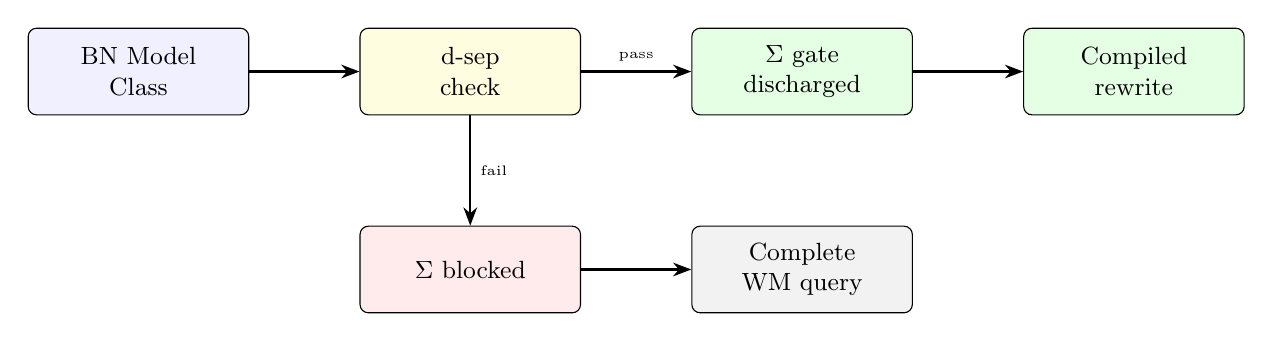
\begin{tikzpicture}[
  >=Stealth,
  every node/.style={font=\small},
  box/.style={draw, rounded corners=3pt, align=center,
              minimum height=11mm, minimum width=28mm},
]
\node[box, fill=blue!6] (model) {BN Model\\Class};
\node[box, fill=yellow!12, right=14mm of model] (dsep) {d-sep\\check};
\node[box, fill=green!10, right=14mm of dsep] (gate) {$\Sigma$ gate\\discharged};
\node[box, fill=green!10, right=14mm of gate] (rule) {Compiled\\rewrite};

\draw[->, thick] (model) -- (dsep);
\draw[->, thick] (dsep) -- node[above, font=\tiny] {pass} (gate);
\draw[->, thick] (gate) -- (rule);

% fail path
\node[box, fill=red!8, below=14mm of dsep] (block) {$\Sigma$ blocked};
\node[box, fill=gray!10, right=14mm of block] (fallback) {Complete\\WM query};

\draw[->, thick] (dsep) -- node[right, font=\tiny] {fail} (block);
\draw[->, thick] (block) -- (fallback);
\end{tikzpicture}
\caption{The $\Sigma$-guarded rewrite pattern.  A compiled rule fires only
when d-separation (or other structural checks) discharge its side conditions.
If the gate is blocked, the system falls back to a complete world-model query
rather than applying an unsound shortcut.}
\label{fig:sigma-guarded-flow}
\end{figure}

\section{The Xi Rule Registry}

The codebase maintains a registry of compiled rewrites covering the four
exact-track rules---deduction, source/induction, sink/abduction, and
revision.  Each rule carries its screening-off side conditions, OSLF atom
bridges, typed BN constructor lifts (chain, fork, or collider), and
coordinate-specialized endpoints for lower, upper, credibility, width,
and strength projections.

See \codepath{Mettapedia/Logic/PLNXiRuleRegistry.lean} and
\codepath{Mettapedia/Logic/PLNBNCompilation.lean}.

\section{Compiled Tactics vs.\ Foundational Semantics}

It is worth pausing to be explicit about the relationship between compiled
rewrites and the foundational calculus.

A compiled rewrite is \emph{admissible}: it can be derived from the
foundational rules plus the structural assumptions in $\Sigma$.  It is
not a new axiom.  It is a theorem that, under stated conditions, a certain
query can be answered by combining the answers to simpler queries.

The advantage of presenting rules as compiled tactics rather than primitive
laws is that the assumptions become visible.  When a PLN deduction rule
``works'' in practice, it is because the implicit BN structure satisfies
the screening-off conditions.  When it ``fails'' (produces incorrect
probabilities), it is because those conditions are violated.  \xiPLN{}
makes this explicit.  These are not ad hoc patches to rescue a broken
rule; they are the actual theoremic scope conditions under which the
classical extensional formulas are exact.


\chapter{Bayesian-Network World Models and Compiled BN Inference}
\label{ch:bn-models}

\begin{quote}\small
\textbf{Goal:} Restrict to BN-structured world models; compile chain/fork/collider inference.\\
\textbf{Semantic object:} BN world-model class; proof-carrying contraction; probabilistic guards.\\
\textbf{Proved:} Chain/fork/collider exactness; guarded admissibility on Pathfinder/Hailfinder.\\
\textbf{Assumed:} BN factorization (declared model class).
\end{quote}

The complete world-table \JointEvidence{} is exponential in $n$.  To scale,
we restrict the world-model class while preserving correctness relative
to the restriction.

\section{BN World-Model Class}

A Bayesian-network world model consists of a directed acyclic graph (DAG)
specifying the factorization, together with local conditional probability
tables (CPTs) whose rows carry Dirichlet evidence counts.  Revision is
the addition of local Dirichlet counts---the conjugate update familiar
from Bayesian statistics---and query answering proceeds by exact inference
via variable elimination or junction tree algorithms.

The DAG structure provides the structural assumptions ($\Sigma$) needed
for compiled rewrites.  D-separation in the DAG determines which
conditional independence assumptions hold, and these determine which
PLN rules are applicable.

See \codepath{Mettapedia/Logic/PLNBayesNetWorldModel.lean}.

\section{Exact BN Query Bridge}

The BN world-model layer provides an evidence plumbing stack that
connects the joint posterior to node-level inference.  At the bottom sits
a Boolean BN CPT query type \code{CPTQuery}, identifying a node together
with its parent configuration.  Above it, a CPT posterior state
\code{CPTState} stores \Evidence{} per CPT entry.  The stack is completed
by an additive projection from \JointEvidence{} to CPT evidence that
marginalizes by summing compatible worlds---and, crucially, this
projection commutes with revision, so that updating the joint and then
projecting gives the same result as projecting first and updating locally.

\section{Chain, Fork, and Collider Exactness}

The three fundamental BN motifs each yield exactness theorems for the
corresponding PLN rule.  Recall the PLN deduction strength formula
(Chapter~\ref{ch:posterior-state}):
\[
  s_{AC} = s_{AB} \cdot s_{BC} + (1 - s_{AB}) \cdot
  \frac{s_C - s_B \cdot s_{BC}}{1 - s_B}
\]

\begin{theorem}[Chain BN deduction exactness (\claimConditional{})]
\label{thm:chain-exact}
In a chain BN $A \to B \to C$ with CPT-based local probabilities,
the screening-off conditions
\[
  P(C \mid A \cap B) = P(C \mid B), \qquad
  P(C \mid A \cap B^c) = P(C \mid B^c)
\]
hold by d-separation.  Under positivity ($P(B \mid A) > 0$, $P(B) \in (0,1)$),
the PLN deduction formula computes the exact conditional:
\[
  s_{AC} = P(C \mid A) = \sum_b P(C \mid B=b) \cdot P(B=b \mid A)
\]
The key mechanism: the CPT row for $C$ depends only on $B$'s value
(sink property), and the joint weight factorizes as
$w(c, r) = P_{\mathrm{CPT}}(c \mid \mathrm{pa}(C)) \cdot
\prod_{v \ne C} P_{\mathrm{CPT}}(v \mid \mathrm{pa}(v))$,
where the second factor is independent of~$c$.
\end{theorem}

\begin{theorem}[Fork BN deduction exactness (\claimConditional{})]
\label{thm:fork-exact}
In a fork BN $A \leftarrow B \to C$, the common-cause $B$ screens off
$A$ from $C$: $P(C \mid A, B) = P(C \mid B)$.  Under positivity, the
PLN deduction formula again yields the exact $P(C \mid A)$.
\end{theorem}

\begin{theorem}[Collider screening-off (\claimConditional{})]
In a collider $A \to B \leftarrow C$, $A$ and $C$ are marginally
independent but become dependent when conditioning on $B$.  The PLN
abduction formula applies with modified side conditions.
\end{theorem}

These ``fast rule exactness'' results show that classic PLN formulas are
not approximations but exact computations within the declared model class.
The screening-off and positivity hypotheses are part of the mathematical
statement, and the local-completeness no-go theorem explains why they
cannot be erased in the unrestricted setting.

See \codepath{Mettapedia/Logic/PLNBayesNetFastRules.lean} and
\codepath{Mettapedia/Logic/PLNXiDerivedBNRules.lean}.

\section{Class-Packaged BN Discharge}

For practical use, the individual screening-off and positivity conditions
are packaged into class-level discharge:
\begin{lstlisting}
allDiscreteCPTLocalMarkov_of
wmqueryeq_of_dsep_discharge_via_soundness_allLocalMarkov
chain_screeningOff_wmqueryeq_of_dsep_allLocalMarkov
fork_screeningOff_wmqueryeq_of_dsep_allLocalMarkov
collider_screeningOff_wmqueryeq_of_dsep_allLocalMarkov
\end{lstlisting}

This means: given a BN model class satisfying local Markov properties,
the screening-off conditions for chain, fork, and collider patterns are
automatically discharged.

See \codepath{Mettapedia/Logic/PLNBNLocalMarkovPackages.lean}.

\section{Worked Proof-Carrying Contraction}

The natural question at this point is whether anything recognizably
PLN-like remains at the operational level.  The answer is yes, but in a
corrected form.  By \emph{proof-carrying contraction} I mean a compiled
rewrite together with its explicit side-condition package $\Sigma$ and
its theorem provenance.  The semantic factor graph is still the
truthmaker; the PLN rule is the local contraction that is allowed to fire
only when $\Sigma$ is discharged.  What disappears is naked truth-value
propagation without a declared model class.

Our canonical worked micro-example is the binary BN
\[
  A \leftarrow H \to B \to C \to D
\]
with
\[
  P(H{=}1)=\tfrac15,\;
  P(A{=}1 \mid H{=}1)=\tfrac9{10},\;
  P(A{=}1 \mid H{=}0)=\tfrac1{10},
\]
\[
  P(B{=}1 \mid H{=}1)=\tfrac45,\;
  P(B{=}1 \mid H{=}0)=\tfrac15,\;
  P(C{=}1 \mid B{=}1)=\tfrac{17}{20},\;
  P(C{=}1 \mid B{=}0)=\tfrac3{20},
\]
\[
  P(D{=}1 \mid C{=}1)=\tfrac9{10},\qquad
  P(D{=}1 \mid C{=}0)=\tfrac1{10}.
\]
The semantic baseline is exact factor-graph elimination on this declared
model.  The compiled PLN-style contractions then recover the same answers
in the exact fragment.  First, a fork-style contraction (the ``source
rule'') reasons from the common-cause motif $A \leftarrow H \to B$ and
obtains $P(B{=}1 \mid A{=}1)=\tfrac8{13}\approx 0.615$.  Next, a
chain-style contraction uses the derived $A \Rightarrow C$ query through
the $B$-mediated exact fragment, yielding
$P(C{=}1 \mid A{=}1)=\tfrac{151}{260}\approx 0.581$.  A second
chain-style contraction then pushes through~$C$ to reach
$P(D{=}1 \mid A{=}1)=\tfrac{367}{650}\approx 0.565$.

The important point is not just the numbers.  Each derived step is
packaged as
\[
  (\text{query}, \text{value}, \Sigma, \text{provenance}),
\]
not as a bare derived edge.  In the Lean demo this provenance points back
to the already-proved exact endpoints
\code{PLNEndToEnd.forkFormulaExact},
\code{PLNEndToEnd.chainFormulaExact}, and the corresponding
$\Sigma$-guarded rewrite surfaces.  See
\code{fork\_contraction\_matches\_exact\_semantics},
\code{chain\_contraction\_C\_matches\_exact\_semantics},
\code{chain\_contraction\_D\_matches\_exact\_semantics} in
\codepath{Mettapedia/Logic/PLNProofCarryingContractionDemo.lean}.

The same file also contains two negative controls, because a worked
positive example is only convincing if it does not quietly smuggle back
the old unrestricted semantics.

First, perturb the fixture so that $C$ depends weakly on $A$ as well as
$B$:
\[
  P(C{=}1 \mid A{=}0,B{=}0)=\tfrac3{20},\;
  P(C{=}1 \mid A{=}1,B{=}0)=\tfrac14,
\]
\[
  P(C{=}1 \mid A{=}0,B{=}1)=\tfrac{17}{20},\;
  P(C{=}1 \mid A{=}1,B{=}1)=\tfrac9{10}.
\]
Now the exact semantic answer becomes
\[
  P(C{=}1 \mid A{=}1)=\tfrac{13}{20}=0.65,
\]
while the naive screened-off contraction gives only
\[
  \tfrac{133}{221}\approx 0.602.
\]
So the gate matters: when $\Sigma$ is not discharged, the exact compiled
chain contraction should not fire.  See
\code{soft\_gate\_blocks\_exact\_contraction} in
\codepath{Mettapedia/Logic/PLNProofCarryingContractionDemo.lean}.

Second, a collider negative control keeps the old abduction story honest.
For the OR-gate collider $A \to C \leftarrow B$ with
$P(A{=}1)=P(B{=}1)=\tfrac12$, the old naive abduction formula yields
$\tfrac23$, while the exact semantic answer remains $\tfrac12$.  So the
refounded system does \emph{not} license free abduction-style link
creation merely because a local pattern ``looks like'' a classic PLN
rule.  See \code{collider\_negative\_control\_blocks\_naive\_abduction} in
\codepath{Mettapedia/Logic/PLNProofCarryingContractionDemo.lean}.

This is the corrected operational reading of PLN rule firing.  The old
intuition survives, but as admissible, $\Sigma$-guarded local contraction
inside a declared world-model class, not as unconstrained link
propagation.

Figure~\ref{fig:proof-carrying-contraction-school} gives the same story in a
simple school-grounded picture.  The left panel is the exact fragment; the
middle panel shows the extra path that blocks the naive chain contraction; the
right panel is the collider negative control.

\begin{figure}[H]
\centering
\begin{subfigure}[t]{0.94\textwidth}
\centering
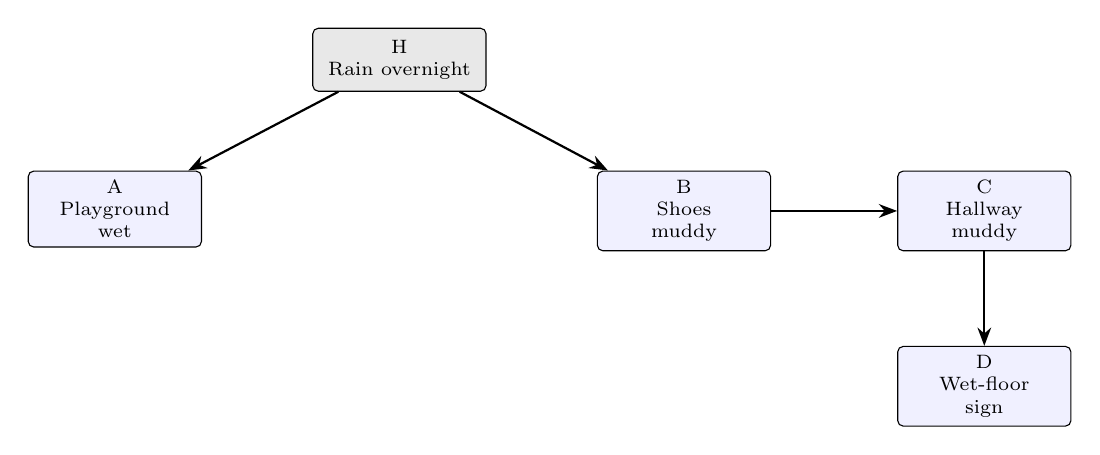
\begin{tikzpicture}[
  >=Stealth,
  node distance=10mm and 14mm,
  every node/.style={font=\scriptsize},
  obs/.style={draw, rounded corners=2pt, fill=blue!6, align=center, minimum width=22mm, minimum height=8mm},
  latent/.style={draw, rounded corners=2pt, fill=gray!18, align=center, minimum width=22mm, minimum height=8mm}
]
\node[latent] (H) {H\\Rain overnight};
\node[obs, below left=of H] (A) {A\\Playground\\wet};
\node[obs, below right=of H] (B) {B\\Shoes\\muddy};
\node[obs, right=16mm of B] (C) {C\\Hallway\\muddy};
\node[obs, below=12mm of C] (D) {D\\Wet-floor\\sign};
\draw[->, thick] (H) -- (A);
\draw[->, thick] (H) -- (B);
\draw[->, thick] (B) -- (C);
\draw[->, thick] (C) -- (D);
\end{tikzpicture}
\caption{Exact fragment: the compiled fork and chain contractions are allowed to fire.}
\end{subfigure}

\medskip
\begin{subfigure}[t]{0.94\textwidth}
\centering
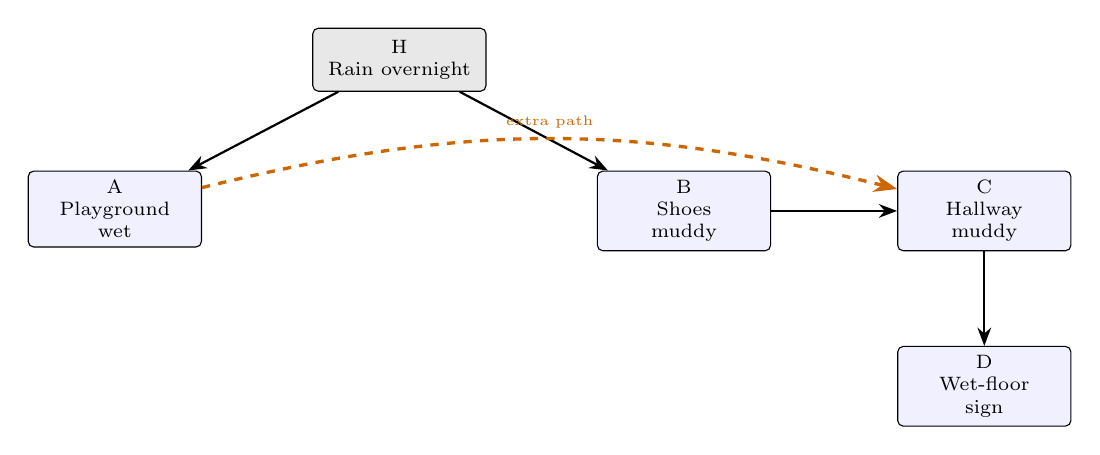
\begin{tikzpicture}[
  >=Stealth,
  node distance=10mm and 14mm,
  every node/.style={font=\scriptsize},
  obs/.style={draw, rounded corners=2pt, fill=blue!6, align=center, minimum width=22mm, minimum height=8mm},
  latent/.style={draw, rounded corners=2pt, fill=gray!18, align=center, minimum width=22mm, minimum height=8mm}
]
\node[latent] (H) {H\\Rain overnight};
\node[obs, below left=of H] (A) {A\\Playground\\wet};
\node[obs, below right=of H] (B) {B\\Shoes\\muddy};
\node[obs, right=16mm of B] (C) {C\\Hallway\\muddy};
\node[obs, below=12mm of C] (D) {D\\Wet-floor\\sign};
\draw[->, thick] (H) -- (A);
\draw[->, thick] (H) -- (B);
\draw[->, thick] (B) -- (C);
\draw[->, thick] (C) -- (D);
\draw[->, dashed, very thick, orange!80!black] (A) to[bend left=14] node[above, font=\tiny] {extra path} (C);
\end{tikzpicture}
\caption{Soft-gate perturbation: a direct playground$\to$hallway path means the chain gate is no longer discharged.}
\end{subfigure}

\medskip
\begin{subfigure}[t]{0.68\textwidth}
\centering
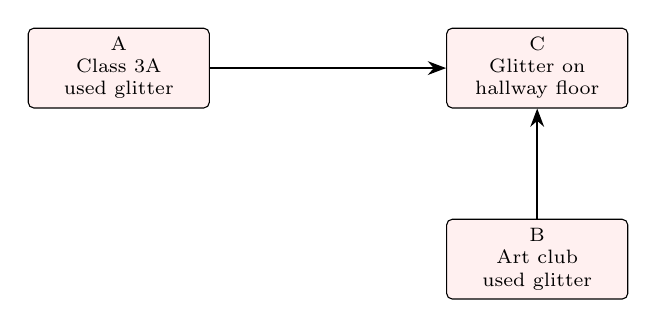
\begin{tikzpicture}[
  >=Stealth,
  node distance=12mm and 14mm,
  every node/.style={font=\scriptsize},
  obs/.style={draw, rounded corners=2pt, fill=red!6, align=center, minimum width=23mm, minimum height=8mm}
]
\node[obs] (A) {A\\Class 3A\\used glitter};
\node[obs, right=30mm of A] (C) {C\\Glitter on\\hallway floor};
\node[obs, below=14mm of C] (B) {B\\Art club\\used glitter};
\draw[->, thick] (A) -- (C);
\draw[->, thick] (B) -- (C);
\end{tikzpicture}
\caption{Collider negative control: seeing the glitter does not license naive free abduction from one source to the other.}
\end{subfigure}
\caption{Elementary-school grounding of the proof-carrying contraction demo.  Left: rain explains both a wet playground and muddy shoes, so the fork/chain contractions match exact semantic inference.  Middle: if the wet playground can also muddy the hallway directly, the naive screened-off contraction is blocked.  Right: two possible glitter sources feeding one hallway clue form a collider, so the old unrestricted abduction intuition must be guarded.}
\label{fig:proof-carrying-contraction-school}
\end{figure}

\subsection{Probabilistically Guarded Admissibility on Real BN Benchmarks}

The toy fixture above establishes the theorem-backed exact fragment in a
fully worked micro-example.  The next question is whether the same
discipline helps on canonical benchmark BNs.  Pathfinder is a classic
Bayesian expert system for diagnosing lymph-node diseases from pathology
findings,\cite{Heckerman1992Pathfinder} and Hailfinder is a Bayesian
severe-weather forecasting model for northeastern Colorado built from
meteorological variables and expert judgment.\cite{Abramson1996Hailfinder}
We use the canonical BIF encodings distributed through the bnlearn
Bayesian Network Repository as the exact BN truthmaker for these
experiments.\cite{ScutariBnRepository} We therefore evaluate Pathfinder
and Hailfinder against exact variable elimination from the BIF
truthmaker, while keeping the derived object discipline explicit:
\smallskip

Throughout this subsection, we use three plain-English labels for the
side-condition context $\Sigma$:
\begin{itemize}
\item \textbf{context-complete}: the carried $\Sigma$ contains the
  structural context needed to license the rewrite exactly;
\item \textbf{context-missing}: some required context has been omitted,
  so the exact rewrite is no longer licensed;
\item \textbf{context-uncertain}: the required context is only
  partially supported, so bounded or operational control layers become
  relevant.
\end{itemize}

\begin{table}[ht]
\centering
\footnotesize
\renewcommand{\arraystretch}{1.04}
\begin{tabular}{@{}p{0.14\textwidth}p{0.18\textwidth}p{0.19\textwidth}p{0.20\textwidth}p{0.21\textwidth}@{}}
\toprule
Benchmark & Domain & Primary artifact & What the variables mean & Why we use it here \\
\midrule
Hailfinder & Severe summer hail forecasting in northeastern Colorado & A hand-built Bayesian weather-forecast BN with expert CPTs; \code{hailfinder.csv} is secondary to \code{hailfinder.bif} & Meteorological conditions, scenario summaries, and forecast targets & Readable positive lane: exact local chaining still works on a real forecast network. \\
Pathfinder & Lymph-node pathology diagnosis & A hand-built Bayesian network with expert CPTs and a disease-class root (\code{Fault}) & One latent diagnosis plus many coded pathology findings in the benchmark release & Hidden-context stress test: can proof-carrying contractions survive when crucial diagnostic context is omitted? \\
\bottomrule
\end{tabular}
\renewcommand{\arraystretch}{1}
\caption{What the two benchmark networks are about.  In both cases the primary benchmark object is the Bayesian network itself, not a generic flat table.}
\label{tab:bn-benchmark-intro}
\end{table}

\paragraph{v2 benchmark design.}
The current benchmark (v2) is organized around three physically
separated table families: a \emph{state table} listing every
(path, context-variant) pair; an \emph{action table} enumerating legal
decisions per state (continue-rule, continue-soft, reveal, fallback,
abstain); and an \emph{eval table} containing exact BN ground truth
that is hidden from policy code.  Oracle and blind decision policies
operate on the \emph{same} master state set; the information-set
separation is enforced by physical column projection---the blind
decision CSV physically lacks all exact-probability and
structural-admissibility columns, making oracle leaks impossible by
construction.  Each state carries a \code{query\_kind} tag (broad vs
refined) and a deterministic hash-based \code{split\_id}
(train/val/test) for reproducible cross-validation.

\[
  (\text{query}, \text{value}, \Sigma, \text{provenance}, g?, \delta?,
    \text{fallback}?).
\]
The guarded layer is an inference-control discipline on top of exact BN
semantics, not a replacement for that semantics.

\begin{center}
\fbox{\begin{minipage}{0.92\textwidth}
\textbf{Three-mode guarded admissibility.}
\smallskip
Context-complete $\Sigma$ gives exact firing.  Context-missing $\Sigma$
blocks the contraction.  Context-uncertain $\Sigma$ moves to a bounded
semantic guard or to an explicit soft fallback layer.
\small
\begin{tabular}{@{}p{0.23\textwidth}p{0.67\textwidth}@{}}
\toprule
Mode & Status and returned object \\
\midrule
Hard-gated exact &
\textit{Semantic, theorem-backed.} Fire only when $\Sigma$ is
discharged.  The returned query answer keeps its carried $\Sigma$ and
provenance; there is no reusable bare derived edge. \\
Bounded violation &
\textit{Semantic guard.} Return an estimate plus an explicit certified
radius or interval against the BN truthmaker. \\
Soft-guarded mixture &
\textit{Operational / governance.} Return
$\hat p = g \cdot p_{\mathrm{rule}} + (1-g) \cdot p_{\mathrm{fallback}}$
with explicit fallback.  This is useful for ranking, abstention, and
trigger logic, but it is not automatically the semantic posterior. \\
\bottomrule
\end{tabular}
\end{minipage}}
\end{center}

\paragraph{Task framing.}
Methodologically, the real question is no longer merely ``can we
classify admissibility?''  It is \emph{topology-conditioned
latent-context inference control}: given a source condition and a target
query inside a declared BN truthmaker, should the controller continue by
exact rewrite, softened continuation, bounded continuation, context
reveal, local exact fallback, or abstention?  Topology matters because
it tells us which kinds of approximation assumptions are likely to
survive transport through the graph and which are likely to fail.
Hailfinder is the readable positive lane for this task.  Pathfinder is
the hostile hidden-context lane.

\paragraph{Hailfinder first: readable exact contraction.}
Hailfinder is the cleaner forecasting-structured benchmark.  The exact
variables are meteorological conditions and forecast targets, so the
benchmark reads like an actual forecast/update chain rather than an
opaque medical codebook.  This is the best first example for readers:
it teaches what a proof-carrying local contraction looks like before the
topology becomes adversarial.
\par
The exact forecast chain
\[
  P(\code{MountainFcst}{=}\code{SIG} \mid
    \code{AMInstabMt}{=}\code{Strong}) = 0.5
\]
fires cleanly, and a longer forecast/update path still matches exact BN
semantics:
\[
  P(\code{CapChange}{=}\code{Increasing} \mid
    \code{CldShadeOth}{=}\code{Cloudy}) = 0.508284\ldots
\]
The negative control remains equally important.  In the selected
collider motif, the exact semantic answer is $0.23595\ldots$, but the
hard gate still blocks unrestricted reuse; bounded mode returns the
interval $[0.23595\ldots, 0.27959\ldots]$, and soft mode returns an
explicit operational mixture with semantic fallback.  So Hailfinder says
there is still a real exact forecasting-style chaining fragment, while
the blocked cases preserve the ``yes, but not everywhere'' boundary.

\paragraph{Pathfinder next: the same calculus under hostile topology.}
Pathfinder is the stronger context-heavy benchmark.  In the current BIF
release it has $109$ nodes and $195$ arcs; \code{Fault} has $63$ states
and $106$ outgoing children, and $56$ nodes have multiple parents.  So
omitted context is not a side issue here.  It is the main structural
fact of the dataset.  In the selected motifs, \code{Fault} is the latent
disease hypothesis and the \code{F\ldots} variables are benchmark-coded
pathology findings from the network file.  For exposition, it is often
better to read the main fork/chain path as
\textit{observation $\rightarrow$ bridge $\rightarrow$ downstream
consequence}, with the actual BN names supplied by
Table~\ref{tab:bn-benchmark-motif-glossary}.
\par
The main Pathfinder stress question is therefore not ``does local
chaining ever work?'' but ``what happens to the same local contraction
when hidden diagnostic context is omitted, partially restored, or
completed?''  In the widened suite the same path family is explicitly
tracked across five regime types:
\emph{context-missing}, \emph{alt-support-only}, \emph{hub-only},
\emph{context-pair}, and \emph{oracle-context-complete}.  That is the
second-order object in practice: uncertainty over which
context/admissibility regime the step is really in.
\par
\begin{table}[ht]
\centering
\footnotesize
\renewcommand{\arraystretch}{1.03}
\begin{tabular}{@{}p{0.17\textwidth}p{0.17\textwidth}p{0.24\textwidth}p{0.30\textwidth}@{}}
\toprule
Network & Variable & Reader gloss & Role in the selected motifs \\
\midrule
Hailfinder & \code{AMInstabMt}, \code{InsInMt}, \code{MountainFcst} & Morning mountain instability, mountain instability, mountain forecast & The clean local forecast-update chain. \\
Hailfinder & \code{CldShadeOth}, \code{AreaMesoALS}, \code{CompPlFcst}, \code{CapChange} & Cloud shading, mesoscale-area summary, composite plains forecast, capping change & The longer readable forecast/update path. \\
Hailfinder & \code{AMCINInScen}, \code{CapInScen} & Scenario-specific convective inhibition and cap state & The collider-style negative boundary. \\
Pathfinder & \code{Fault} & Latent disease hypothesis / diagnosis class & The hidden diagnostic context that often has to stay in $\Sigma$. \\
Pathfinder & \code{F3}, \code{F4}, \code{F103} & Benchmark-coded observed pathology clues & Upstream evidence nodes in the selected fork and long-path motifs. \\
Pathfinder & \code{F97}, \code{F105} & Benchmark-coded intermediate pathology factors & Intermediate shared nodes through which the admissible contraction travels. \\
Pathfinder & \code{F101}, \code{F102}, \code{F104} & Benchmark-coded downstream pathology targets & Queried consequences used to test exactness and hidden-context sensitivity. \\
\bottomrule
\end{tabular}
\renewcommand{\arraystretch}{1}
\caption{Mini glossary for the variables actually used in the current benchmark motifs.  Pathfinder keeps the compact benchmark coding from the released network; Hailfinder uses more readable meteorological names.}
\label{tab:bn-benchmark-motif-glossary}
\end{table}

In the selected fork motif, keeping \code{Fault} explicit in $\Sigma$
yields an exact
hard-gated contraction:
\[
\begin{aligned}
P(F104{=}\code{x\_50} \mid {}&F103{=}\code{Almost\_all\_poor\_def}, \\
  &\code{Fault}{=}\code{T\_immunob\_lrg}) = 0.4.
\end{aligned}
\]
But if the same motif is evaluated in the \emph{context-missing} regime,
with \code{Fault} omitted from $\Sigma$, the exact semantic answer drops
to $0.14998\ldots$, and the hard gate blocks.  The bounded mode then
returns the rule estimate
$0.31236\ldots$ together with the certified interval
$[0.14998\ldots, 0.47474\ldots]$, while the soft-gated operational layer
returns $0.28599\ldots$ with explicit fallback to the exact semantic
query.  This is the intended result: Pathfinder does not show that
``free PLN chaining works'' on a large medical BN; it shows that
proof-carrying local contraction survives only when the hidden
diagnostic context is carried, and that context-erasing contractions
must be blocked or degraded gracefully.

\begin{table}[ht]
\centering
\footnotesize
\renewcommand{\arraystretch}{1.04}
\begin{tabular}{@{}p{0.17\textwidth}p{0.10\textwidth}p{0.25\textwidth}p{0.34\textwidth}@{}}
\toprule
Case & Exact BN & Guarded output & Why it matters \\
\midrule
Hailfinder exact forecast chain &
$0.500$ &
Hard fires.\par Bounded $\delta = 0$.\par Soft $g = 1$. &
There is still a clean exact chaining fragment for forecasting-style
paths. \\
Hailfinder forecast collider negative &
$0.236$ &
Hard blocks.\par Bounded $0.258$ in $[0.236, 0.280]$.\par Soft $0.257$. &
The guarded layer preserves the no-free-abduction boundary even in the
forecasting BN. \\
Pathfinder context-complete fork &
$0.400$ &
Hard fires.\par Bounded $\delta = 0$.\par Soft $g = 1$. &
When \code{Fault} stays in $\Sigma$, PLN-style contraction is exact. \\
Pathfinder context-missing fork &
$0.150$ &
Hard blocks.\par Bounded $0.312$ in $[0.150, 0.475]$.\par Soft $0.286$. &
Omitting \code{Fault} changes the answer sharply; carried context is
necessary. \\
\bottomrule
\end{tabular}
\renewcommand{\arraystretch}{1}
\caption{Compact guarded-admissibility summary for the current real BN benchmarks.  Exact BN semantics remains the truthmaker in every row.}
\label{tab:prob-guarded-benchmark-summary}
\end{table}

The next question is why adventurous continuation sometimes wins the
original broad Pathfinder task and sometimes does not.  Here the most
useful abstraction is no longer a single guard score.  It is a
topology-conditioned latent-context controller.  Let $C$ denote
unresolved hidden context, typically including \code{Fault} and, in some
paths, an auxiliary support variable.  Before any reveal action, the
target is the broad query $P(Q \mid E)$.  After revealing one context
value $c$, the target becomes the refined query $P(Q \mid E, C{=}c)$.
These are different tasks.  Exact reveal wins the refined task because
it conditions on the right branch explicitly.  But it need not minimize
error against the original broad task, because the broad query
marginalizes over the still unresolved context:
\[
  P(Q \mid E) = \sum_c P(Q \mid E, C{=}c)\,P(C{=}c \mid E).
\]
A controlled soft continuation,
\[
  \hat p_{\mathrm{soft}} =
  g\,p_{\mathrm{rule}} + (1-g)\,p_{\mathrm{fallback}},
\]
can therefore be a better \emph{operational} estimator for the original
broad query than prematurely collapsing onto a single revealed branch,
even though we do not yet claim that the current learned $g$ is itself
the semantic posterior.  But the widened Pathfinder suite shows that
this is not universal.  The topology label is precisely what tells us
which approximation assumptions are more or less plausible.  In
hub-dominated cases, omitted-context mass is often concentrated around
one dominant diagnostic direction, so direct continuation can stay close
to the unresolved broad marginal.  In loopy-dense or partial-support
cases, several live alternatives can remain active, and then softened or
marginalization-aware continuation becomes more attractive.  So the
current benchmark-side explanation is already informative: topology is
not a decorative covariate but a guide to which kinds of assumptions do
or do not transport well.  The new point is that the finite
regime-mixture layer is now theorem-backed in Lean, in
\code{PLNRegimeMixtureTheorems.lean},
\code{PLNRegimeMixtureBenchmarkBridge.lean},
\code{PLNWorldModelRegimeAdmissibility.lean}, and
\code{PLNProbHOLPlannerBridge.lean}.  If $R$ is a finite regime space,
$w_r$ are posterior regime weights, and $q_r$ are branch query values,
then the unresolved broad-query predictor is
\[
  m = \sum_{r \in R} w_r q_r.
\]
For any designated branch $r_0$, the direct-continuation approximation
error obeys the residual-mass bound
\[
  |m - q_{r_0}| \le (1 - w_{r_0}) \cdot
  \max_{r \neq r_0} |q_r - q_{r_0}|.
\]
Under squared loss, the constant-predictor risk decomposes as
\[
  \sum_{r \in R} w_r (x - q_r)^2
  = \underbrace{\sum_{r \in R} w_r (m - q_r)^2}_{\text{mixture variance}}
    + (x - m)^2,
\]
so the unresolved mixture predictor $m$ is optimal among constant
predictors, and exact reveal is preferred once
\[
  \text{gain}_{\mathrm{reveal}}
  = \text{mixture variance} - c_{\mathrm{reveal}} > 0.
\]
This is already enough to turn the higher-order direct/soft/reveal split
into a theoremic finite-regime statement: direct continuation is
justified when posterior mass concentrates tightly around one branch;
soft continuation is justified because the mixture predictor minimizes
unrevealed squared-loss risk; and reveal/context completion is justified
once value-of-information beats reveal cost.  What remains empirical at
present is the \emph{topology-conditioned proxy story}: labels such as
``hub-dominated'' or ``loopy-dense'' are still benchmark-side ways of
predicting when concentration, spread, and latent support are likely to
take those theoremically relevant shapes.

\paragraph{Three higher-order claims.}
The current benchmark supports three proposition-shaped claims that keep
the semantics/control split clean.
\begin{enumerate}
\item \textbf{Objective mismatch under reveal.} Revealing hidden context
  changes the target from a broad marginalized query to a refined
  conditional query, so reveal can improve refined fidelity while
  worsening broad-query utility.
\item \textbf{Topology-conditioned continuation preference.}
  Hub-dominated slices often reward direct continuation; partial-support
  and some loopy-dense slices leave more live alternatives and therefore
  make softened continuation more competitive.
\item \textbf{Higher-order flattening at decision time.} Even when
  admissibility and trust are modeled explicitly, action choice need not
  recurse through an ever taller explicit tower; it can flatten to
  expected utility, interval dominance, or abstention at decision time.
\end{enumerate}

We now make that higher-order split explicit.  The second-order variable
$G_{\mathrm{step}}$ means ``this local contraction is admissible enough
in the current structural regime'', so the live second-order object is
best read as a regime posterior $\pi(r \mid \text{local state})$ over
hidden-context/admissibility regimes rather than as one free-floating
confidence scalar.  A third-order trust layer then records how much
confidence to place in the current model of $G_{\mathrm{step}}$ for the
present topology/context class.  The point is not infinite regress for
its own sake, but an explicit separation between object-level belief,
admissibility belief, and trust in the admissibility model itself.
Fourth-order and higher concerns are then handled, for the benchmark, as
flattening or robustness questions rather than as an endlessly explicit
tower.  In the widened sweep, Hailfinder
\emph{context-complete} paths have mean third-order meta-trust $0.819$
with reveal pressure $0.147$, while Pathfinder has meta-trust $0.563$
with reveal pressure $0.761$ in the \emph{context-missing} regime,
$0.603/0.545$ in the \emph{alt-support-only} regime,
$0.764/0.184$ in the \emph{context-pair} regime, and
$0.798/0.159$ in the \emph{oracle-context-complete} regime.  So the
planner is not only asking ``can I chain?'' but also ``how much do I
trust my own admissibility estimate here, in this topology and context
class?''  In the current architecture these planner-facing
second-/third-order quantities are intended as empirical control
shadows of the semantic ProbHOL $\rightarrow$ belief-process
$\rightarrow$ planner bridge, not as replacement semantics.

\begin{table}[ht]
\centering
\scriptsize
\renewcommand{\arraystretch}{1.0}
\begin{tabular}{@{}p{0.26\textwidth}p{0.11\textwidth}p{0.12\textwidth}p{0.22\textwidth}p{0.19\textwidth}@{}}
\toprule
Regime slice & Meta-trust & Reveal pressure & Best broad-query action & Best refined-query action \\
\midrule
Hailfinder forecast chain, context-complete &
$0.819$ &
$0.147$ &
\code{Regime-mixture} / exact chain, MAE $0.0000$. &
\code{Regime-mixture} / exact chain, MAE $0.0000$. \\
Pathfinder hub-dominated, context-missing &
$0.590$ &
$0.769$ &
\code{Anchored regime-mixture}, MAE $0.0090$ (one-shot). &
Context-complete / exact fallback, refined MAE $0.0000$. \\
Pathfinder hub-dominated, alt-support-only &
$0.555$ &
$0.596$ &
\code{Anchored regime-mixture}, MAE $0.2584$. &
Context-complete / exact fallback, refined MAE $0.0000$. \\
Pathfinder loopy-dense, context-missing &
$0.548$ &
$0.757$ &
\code{Anchored regime-mixture}, MAE $0.0489$ (one-shot). &
Context-complete / exact fallback, refined MAE $0.0000$. \\
Pathfinder loopy-dense, oracle-context-complete &
$0.926$ &
$0.074$ &
\code{Anchored regime-mixture}, MAE $0.2646$. &
\code{Rule-only}, refined MAE $0.0087$. \\
\bottomrule
\end{tabular}
\renewcommand{\arraystretch}{1}
\caption{Compact topology-conditioned higher-order split in the widened benchmark sweep (v1 prototype; v2 restructured results use the state/action/eval pipeline described below).  One-shot broad-query winners are often anchored regime-mixture actions, while refined-query winners still mostly come from explicit context completion or exact fallback.}
\label{tab:second-third-order-query-split}
\end{table}

Table~\ref{tab:second-third-order-query-split} also shows why the
higher-order story is genuinely interesting rather than merely cautious.
The current benchmark no longer supports the simpler claim that ``soft
continuation wins the hardest broad-query cases''.  Instead, the better
statement is now more precise.  After anchoring the explicit
regime-mixture continuation to the current broad-query branch, the
strongest \emph{one-shot} broad-query action is often the anchored
regime-mixture policy, including the widened Pathfinder
\emph{context-missing} rows.  Mechanistically, the hub-dominated slices
look like unresolved broad queries whose mass is already concentrated in
one main diagnostic direction, so a small anchored mixture smooths the
remaining uncertainty without collapsing to one refined branch.  The
alt-support and loopy slices keep more hidden-context alternatives live,
which is why structured regime averaging helps more than blunt
\code{rule-only} continuation at the one-shot level.  But the stricter
\emph{higher-order chain-composition} benchmark still leaves several
multi-step \emph{context-missing} slices to \code{rule-only} chain
continuation.  So the present result is not ``the planner is solved'',
but ``the broad/refined objective split is real, the best adventurous
one-shot action depends on topology and hidden-context regime, and the
best full-chain action can still be different''.  In this sense,
topology is functioning as a compact summary of which kinds of
independence, concentration, and branch-mixing assumptions are likely to
work in a local region of the graph.

\begin{table}[ht]
\centering
\footnotesize
\renewcommand{\arraystretch}{1.04}
\begin{tabular}{@{}p{0.19\textwidth}p{0.19\textwidth}p{0.12\textwidth}p{0.18\textwidth}p{0.24\textwidth}@{}}
\toprule
Slice & Best broad one-shot policy & Broad MAE & Best full-chain policy & Main takeaway \\
\midrule
Hailfinder forecast chain, context-complete &
\code{Explicit regime-mixture} &
$0.0000$ &
\code{Rule-only} chain (exact) &
In the clean lane the higher-order controller collapses back to the
exact fragment. \\
Pathfinder hub-dominated, context-missing &
\code{Explicit regime-mixture} &
$0.0090$ &
\code{Rule-only} chain &
Anchored regime averaging helps at the one-shot level, but full
multi-step composition still prefers blunt continuation. \\
Pathfinder loopy-dense, context-missing &
\code{Explicit regime-mixture} &
$0.0489$ &
\code{Rule-only} chain &
One-shot smoothing helps, but loopy full-chain continuation still
resists a universal adventurous policy. \\
Pathfinder multi-support revision &
\code{Base-plus-support revision} &
$0.0197$ / $0.0854$ &
-- &
Combining hub/nonhub/pair supports is the clearest PLN-style positive
result on the widened suite (hub-dominated / loopy-dense). \\
Reveal as value of information on Pathfinder context-missing &
Continue for the broad query &
$\Delta_{\mathrm{refined}} = +0.715$ / $+0.067$ &
Reveal only for the refined task &
Reveal improves refined fidelity, but usually solves the wrong task for
the original broad query and incurs large broad-query regret. \\
\bottomrule
\end{tabular}
\renewcommand{\arraystretch}{1}
\caption{Stabilized higher-order benchmark takeaways (v1 prototype; v2 restructured results use the state/action/eval pipeline) after explicit regime-mixture continuation, PLN-style multi-support revision, reveal-as-value-of-information evaluation, and higher-order chain composition.  The two numbers in the multi-support and VOI rows correspond to the hub-dominated and loopy-dense Pathfinder slices respectively.}
\label{tab:stabilized-higher-order-benchmark}
\end{table}

To keep the setup fully auditable, we make the v2-clean protocol explicit here.
The pipeline is a seven-script sequence, each consuming the output of
the previous step:
\code{wm\_pln\_v2c\_build\_master\_suite.py}
$\rightarrow$
\code{wm\_pln\_v2c\_build\_actions.py}
$\rightarrow$
\code{wm\_pln\_v2c\_build\_eval.py}
$\rightarrow$
\code{wm\_pln\_v2c\_project\_views.py}
$\rightarrow$
\code{wm\_pln\_v2c\_train\_blind\_models.py}
$\rightarrow$
\code{wm\_pln\_v2c\_run\_policies.py}
$\rightarrow$
\code{wm\_pln\_v2c\_evaluate.py}.
All scripts live under \codepath{scripts/} and reuse the existing
BN-inference backbone (\code{wm\_pln\_bn\_common.py}),
topology utilities (\code{wm\_pln\_second\_order\_common.py}),
and motif catalogues
(\code{wm\_pln\_pathfinder\_motifs.py},
\code{wm\_pln\_hailfinder\_motifs.py}).
The v2-clean artifacts are written to \codepath{results/v2\_clean/},
with per-dataset state, action, eval, decision-oracle, decision-blind,
policy, and results CSVs.
The v2 prototype is preserved under \codepath{results/v2/} and
the v1 prototype under \codepath{results/v1\_archive/} for provenance.
\par
Five contract-level changes distinguish v2-clean from the v2 prototype:
(1)~\code{oracle\_context\_complete} is removed from the shared
decision substrate---only blind-legitimate context variants appear;
(2)~reveal is a \emph{real transition}: the controller pays the reveal
cost and the follow-up action is evaluated on the target state's exact
BN ground truth (with a penalty for EXTERNAL or missing targets);
(3)~path-family--level splits guarantee nonempty train/val/test partitions,
and headline numbers report test-only results;
(4)~blind learning is \emph{action-conditional}: XGBoost predicts
per (state, action) pair, not per state, so different actions from the
same state receive different \code{g\_hat\_action\_error} predictions;
(5)~oracle and blind decision views are \emph{physically separate}
CSV projections---the blind view cannot contain oracle columns.
\par
The policy set covers both oracle and blind lanes:
\code{adaptive\_oracle}/\code{adaptive\_blind},
\code{force\_rule\_only},
\code{force\_soft},
\code{force\_reveal},
\code{force\_fallback}, and
\code{force\_abstain}.
Both lanes operate on the same $50$~Pathfinder +
$45$~Hailfinder master state set ($95$ states total).
\par
The scoring function used by the regime-mixture and chain benchmarks is
\[
\text{score}
=
1
- 2\cdot \text{primary-error}
- 0.08\cdot \text{plan-cost}
- \lambda_{\text{reveal}}\cdot \#\text{reveals},
\]
with $\lambda_{\text{reveal}}=0.05$ (a single balanced objective).
Action-cost parameters are
\[
\begin{aligned}
\text{hard} &= 0.8 + 0.6\cdot \text{edges},\\
\text{guarded} &= 0.6 + 0.4\cdot \text{edges},\\
\text{fallback} &= 2.0 + 0.8\cdot \text{edges},\\
\text{reveal} &= 0.7\cdot \#\text{missing-required-context-vars}.
\end{aligned}
\]
\par
Pathfinder topology labels are assigned directly from local graph
statistics in the benchmark scripts:
\emph{hub-dominated} if \code{Fault} is on-path or max node degree
$\ge 50$; \emph{loopy-dense} if downstream multi-parent count $\ge 2$ or
mean local branching $\ge 4$.
The v2-clean Pathfinder suite has $10$ path families
($4$ anchors + $6$ discovered) expanded into $50$ states via $5$
blind-legitimate context variants (context-missing, hub-only,
context-partial, alternating-partial, nonhub-only).
The Hailfinder suite has $9$ motif families ($5$ exact chains/forks,
$2$ long paths, $2$ collider negatives) expanded into $45$ states.
The $95$ total states span both topology classes
(hub-dominated and loopy-dense Pathfinder slices;
all Hailfinder motifs are tree-like or sparse-chain-like) and all
blind-legitimate context completeness levels.
The blind guard model is trained via XGBoost + isotonic calibration
on topology-derived features (path length, max node degree, sigma
count, context completeness) \emph{plus} action-level features
(action type, cost, reveal metadata) to predict action-conditional
error from the blind decision view alone.

\begin{table}[ht]
\centering
\footnotesize
\renewcommand{\arraystretch}{1.03}
\begin{tabular}{@{}lrrrrrrr@{}}
\toprule
Slice & Rows & Groups & Hard & Blocked & $\epsilon$-exact & ECE iso$\to$conf & Brier iso$\to$conf \\
\midrule
Hailfinder coverage & 62 & 62 & 0.629 & 0.371 & 0.758 & 0.205$\to$0.205 & 0.188$\to$0.188 \\
Pathfinder coverage & 145 & 80 & 0.448 & 0.552 & 0.634 & 0.074$\to$0.074 & 0.064$\to$0.064 \\
Cross H$\to$P guard transfer & 145 & -- & 0.448 & 0.552 & 0.634 & 0.323$\to$0.190 & 0.307$\to$0.237 \\
Cross P$\to$H guard transfer & 62 & -- & 0.629 & 0.371 & 0.758 & 0.119$\to$0.110 & 0.118$\to$0.117 \\
\bottomrule
\end{tabular}
\renewcommand{\arraystretch}{1}
\caption{Motif-coverage and calibrated guard-transfer summary (v1 prototype; v2 uses the state/action/eval pipeline with physical column projection).
``Hard'' and ``Blocked'' are structural admissibility rates;
$\epsilon$-exact uses $\epsilon=0.02$. The conformal guard is operational
confidence shaping, not posterior semantics.}
\label{tab:prob-guarded-coverage-calibration}
\end{table}

For these real-network cases, the bounded mode is currently
\emph{evaluation-certified} from the exact BN truthmaker rather than
derived from a general theoremic bound calculus over arbitrary BNs.
That limitation should be read as a strength of the presentation rather
than a weakness: the semantic anchor stays exact, and the guarded layer
is explicit about where it is theorem-backed, where it is certified by
comparison against the truthmaker, and where it is merely operational.

\begin{center}
\fbox{\begin{minipage}{0.92\textwidth}
\textbf{Reproducibility block (v2-clean pipeline).}
\small
\textit{Scripts} (run in order):\\
\codepath{scripts/wm\_pln\_v2c\_build\_master\_suite.py}\\
\codepath{scripts/wm\_pln\_v2c\_build\_actions.py}\\
\codepath{scripts/wm\_pln\_v2c\_build\_eval.py}\\
\codepath{scripts/wm\_pln\_v2c\_project\_views.py}\\
\codepath{scripts/wm\_pln\_v2c\_train\_blind\_models.py}\\
\codepath{scripts/wm\_pln\_v2c\_run\_policies.py}\\
\codepath{scripts/wm\_pln\_v2c\_evaluate.py}

\smallskip
\textit{Results (test-only headlines).}
\codepath{results/v2\_clean/pathfinder\_states.csv} (50 states)\\
\codepath{results/v2\_clean/hailfinder\_states.csv} (45 states)\\
\codepath{results/v2\_clean/*\_decision\_oracle.csv} (all columns)\\
\codepath{results/v2\_clean/*\_decision\_blind.csv} (topology + action features)\\
\codepath{results/v2\_clean/*\_results.csv} (per-state evaluation)\\
\codepath{results/v2\_clean/*\_results\_summary\_test.csv} (test-only)\\
\codepath{results/v2\_clean/guard\_model/} (blind XGBoost artifacts)\\
\codepath{results/v2\_clean/benchmark\_contract\_audit.txt}

\smallskip
\textit{Lean theory.}
\codepath{Mettapedia/Logic/PLNProbGuardedAdmissibilityDemo.lean}\\
\codepath{Mettapedia/Logic/PLNProbGuardedAdmissibilityRegression.lean}

\smallskip
\textit{Prior versions.}
\codepath{results/v2/} (v2 prototype baseline)\\
\codepath{results/v1\_archive/} (v1 superseded results)
\end{minipage}}
\end{center}

\paragraph{Related benchmark literature.}
The Pathfinder and Hailfinder networks originate from the bnlearn
repository~\cite{ScutariBnRepository} and have long served as test cases
for exact BN inference algorithms.  Standard BN inference benchmarks
(e.g.\ the UAI approximate inference competitions, ProbModelS) evaluate
\emph{inference algorithm quality}---how accurately a solver recovers
posterior marginals.  Our benchmark evaluates a different object:
\emph{inference control quality}---given an inference engine that can
already compute exact posteriors, how well does a higher-order
controller decide when to continue, soften, reveal context, fall back,
or abstain?  This control-level evaluation is closer in spirit to active
learning and value-of-information frameworks than to solver benchmarks.
The blind guard model connects to conformal prediction as the
distribution-free bridge from learned topology features to certified
admissibility estimates.

\subsection{Hetionet / Rephetio: the next flagship benchmark}

At this point the project has three ingredients in place.  First, the
Pathfinder/Hailfinder lane already gives us a real small-to-medium
benchmark story for exact contraction, guarded continuation, reveal as
value of information, multi-support revision, and higher-order chain
composition.  Second, Chapter~11 now exposes the semantic
ProbHOL $\rightarrow$ belief-process $\rightarrow$ planner-shadow bridge
as the canonical waist of the architecture.  Third, we now have a
concrete large-scale benchmark candidate in hand: the Hetionet /
Rephetio drug-repurposing stack.\cite{Himmelstein2017Rephetio,DhimmelHetioRepData}
The motive for moving there is simple.  Hetionet is large, typed,
path-rich, and explanation-oriented, so it is a better stress test of
higher-order chaining than another toy relational dataset.  It is also
already rich enough that there is no single clean leaderboard; instead
there is a cluster of benchmark traditions with different task
definitions, path semantics, explanation targets, and reproducibility
caveats.\cite{Liu2021NeuralMultiHopBioKG,Jimenez2024XG4Repo,Himmelstein2022HetnetConnectivity,Nunes2024RExDrugRepurposing,Bonner2022KGEDrugDiscovery,PerdomoQuinteiro2024KGDrugRepurposingReview,KGScopingReview2025DrugRepurposing}

\begin{table}[ht]
\centering
\scriptsize
\renewcommand{\arraystretch}{1.02}
\begin{tabular}{@{}p{0.18\textwidth}p{0.22\textwidth}p{0.20\textwidth}p{0.25\textwidth}@{}}
\toprule
Paper & Role for this project & What it contributes & Main caution \\
\midrule
Rephetio / Hetionet \cite{Himmelstein2017Rephetio} &
Canonical benchmark definition &
Defines the graph, the \code{Compound-treats-Disease} target, and the
metapath / DWPC setup. &
Original setup is not itself a higher-order control benchmark. \\
PoLo-style logical multi-hop \cite{Liu2021NeuralMultiHopBioKG} &
Closest chaining comparator &
Shows that typed logical multi-hop reasoning on biomedical KGs is a real
comparison class. &
Not the same semantic / reveal / regime split as our WM lane. \\
XG4Repo \cite{Jimenez2024XG4Repo} &
Explainable path-completion comparator &
Direct path-based Hetionet drug-repurposing benchmark with rule and RL
comparisons. &
Reported Hetionet test slices are small, so hard SOTA claims are shaky. \\
Hetnet connectivity search \cite{Himmelstein2022HetnetConnectivity} &
Unsupervised path-family discovery &
Finds degree-adjusted important path families without a supervised gold
label. &
Analysis tool, not a full continuation controller. \\
REx \cite{Nunes2024RExDrugRepurposing} &
Explanation-ranking comparator &
Benchmarks explanatory path quality using Hetionet-style drug
repurposing hypotheses. &
Optimizes explanation quality rather than the broad/refined control
tradeoff directly. \\
Bonner et al.\ \cite{Bonner2022KGEDrugDiscovery} &
Benchmark-sensitivity warning &
Shows that ranking changes materially with split, hyperparameters, and
seed. &
Raw score-chasing without protocol control is misleading. \\
Reviews \cite{PerdomoQuinteiro2024KGDrugRepurposingReview,KGScopingReview2025DrugRepurposing} &
Broader field orientation &
Situate Hetionet among larger drug-repurposing KGs and method families. &
Useful context, but not benchmark semantics by themselves. \\
\bottomrule
\end{tabular}
\renewcommand{\arraystretch}{1}
\caption{Research landscape for the next large-scale benchmark.  The right reading is not ``one SOTA leaderboard'', but a cluster of benchmark traditions around path reasoning, explanation, and evaluation protocol.}
\label{tab:hetionet-research-landscape}
\end{table}

The dataset itself also needs to be described clearly, because the
benchmark object is not one flat table.  Hetionet is the heterogeneous
biomedical graph; Rephetio is the benchmark-facing drug-repurposing
layer built on top of it.  In the current public browser-table bundle we
have a typed graph with $47{,}031$ nodes, $2{,}250{,}197$ relationships,
and $24$ edge types, together with benchmark-facing tables for $1{,}538$
compounds, $136$ diseases, $1{,}206$ metapaths, $1{,}000$
compound-conditioned prediction tables, and $136$
disease-conditioned prediction tables.\cite{Himmelstein2017Rephetio,DhimmelHetioRepData}
This is exactly the shape we want: small enough to inspect, large enough
to matter, and rich enough that typed multi-hop support families are not
an afterthought.

\begin{table}[ht]
\centering
\scriptsize
\renewcommand{\arraystretch}{1.02}
\begin{tabular}{@{}p{0.20\textwidth}p{0.31\textwidth}p{0.33\textwidth}@{}}
\toprule
Artifact & What it contains & Why it matters for HO chaining \\
\midrule
Hetionet graph &
$47{,}031$ nodes, $2{,}250{,}197$ relations, $24$ edge types &
Semantic heterogeneous substrate and typed path space. \\
Rephetio compounds table &
$1{,}538$ compounds, with $755$ treatments and $390$ palliations &
Compound-side query inventory and positive label counts. \\
Rephetio diseases table &
$136$ diseases, with the same treatment/palliation support counts &
Disease-side query inventory and target coverage. \\
Rephetio metapaths table &
$1{,}206$ metapaths of length $2$--$4$, with $\Delta$AUROC and fitted coefficients &
Typed support families and regime candidates. \\
Per-compound predictions &
$1{,}000$ tables, each scoring one compound against all diseases &
Broad compound-conditioned support surface. \\
Per-disease predictions &
$136$ tables, each scoring one disease against all compounds &
Disease-conditioned scoring and explanation surface. \\
\bottomrule
\end{tabular}
\renewcommand{\arraystretch}{1}
\caption{What the Hetionet / Rephetio benchmark actually consists of in the current public bundle.  The graph is the heterogeneous biomedical substrate; the Rephetio tables provide the benchmark-facing task surface.}
\label{tab:hetionet-dataset-surface}
\end{table}

The flagship query for this benchmark is
\[
  \code{treats}(\textit{compound}, \textit{disease}).
\]
The methods/motives follow directly from the work already in hand.
Pathfinder and Hailfinder taught us that the interesting control problem
is not merely whether a local step is exact, but how to act when context
is incomplete, several support families are live, and reveal can change
the target from a broad unresolved query to a refined conditional one.
Hetionet / Rephetio is where that question becomes typed and large-scale.
For example, metapaths such as
\code{CbGaD} (Compound--binds--Gene--associates--Disease),
\code{CrCtD} (Compound--resembles--Compound--treats--Disease), and
\code{CiPCiCtD} (Compound--includes--Pharmacologic Class--includes--Compound--treats--Disease)
already look like natural higher-order support families rather than
accidental path fragments.
\par
The planned protocol therefore proceeds in four stages.  First,
\emph{one-shot regime-mixture continuation} treats typed
metapath/support families as second-order regimes and compares
\code{rule-only}, explicit regime-mixture continuation, reveal, and
fallback on the broad \code{treats(c,d)} task.  Second,
\emph{PLN-style multi-support revision} combines several live support
families for the same query with explicit overlap penalties or residual
ignorance terms, rather than pretending free independence.  Third,
\emph{reveal as value of information} asks when inspecting an additional
mechanism family or context slice improves refined fidelity enough to
justify its cost---instead of silently changing the target.  Fourth,
\emph{higher-order chain composition} evaluates whether the guarded
continuation machinery survives over interpretable
compound--gene--disease and compound--compound--disease chains, not just
one-shot scoring.
At the semantic level, the split is the same as in the current
benchmark lane:
\begin{itemize}
\item \textbf{1st order}: support for \code{treats(c,d)};
\item \textbf{2nd order}: uncertainty over metapath/context/support
  regime;
\item \textbf{3rd order}: trust in the regime estimator;
\item \textbf{4th and beyond}: flattened to expected utility, interval
  dominance, or abstention at action time.
\end{itemize}
This means the next benchmark consumer is already aligned with the
Chapter~11 architecture:
\[
  \text{truth}
  \to \text{hierarchical semantic probability}
  \to \text{belief tracking}
  \to \text{planner shadow}.
\]
What we are \emph{not} claiming yet is equally important.  This section
does not report finished Hetionet results, and it does not treat the
Rephetio browser tables as a semantic oracle by themselves.  Rather, it
states the next flagship benchmark plan now that the semantic
ProbHOL $\rightarrow$ belief $\rightarrow$ planner waist is finally in
place: the benchmark-side regime and trust fields should become
principled projections of that bridge, not one more layer of bespoke
scores.

\subsection{GWAS locus-to-gene: replication-first benchmark lane}

The genomic lane should be staged with the same discipline.  The relevant
benchmark object is not merely ``some SNP--gene scores,'' but a full
locus-to-gene pipeline with at least three separable layers:
\begin{enumerate}
\item the \emph{scientific task} (candidate gene ranking for a variant or
  locus, and later variant $\to$ gene $\to$ mechanism explanation);
\item the \emph{scoring semantics} (the current ProbLog/LPAD baseline versus a
  WM-PLN evidence-carrying strengthening); and
\item the \emph{runtime surface} (native repo/cplint path first, Janus/PeTTa
  parity second, any later harnesses only after that).
\end{enumerate}
That separation matters because the public
\codepath{hypothesis-generation-demo} repository already contains its own
benchmark-facing ProbLog family: a learned-rule LPAD surface in
\codepath{pl/pl\_rules.pl}, a native cplint parameter-learning/evaluation
driver in \codepath{pl/param\_learn.pl}, and the current fold/index artifacts
under \codepath{pl/models/}.  So the first obligation is not to replace that
surface with a new one.  It is to replicate their methodology with
\emph{their} ProbLog stack as faithfully as the surviving data/runtime
artifacts allow.

\begin{table}[ht]
\centering
\scriptsize
\renewcommand{\arraystretch}{1.02}
\begin{tabular}{@{}p{0.22\textwidth}p{0.31\textwidth}p{0.31\textwidth}@{}}
\toprule
Surface / bundle & What we currently have locally & Role in the benchmark plan \\
\midrule
Native repo artifacts &
\codepath{pl/param\_learn.pl}, \codepath{pl/pl\_rules.pl}, five
\codepath{pl/models/fold\_\*/} partitions, and stored ROC/PR charts &
Primary replication target: this is the original LPAD/cplint methodology we
should reproduce before claiming any WM improvement. \\
Public-source genomic reconstruction &
GTEx v8 eQTL data~\cite{GTEx2020}, ABC enhancer predictions~\cite{Nasser2021ABC},
chr16 GeneHancer/cache material, SNP/gene coordinate caches, and the narrower
genomic note's reconstructed feature bundle &
Methodology-replication substrate if the original compiled Prolog KB snapshot
cannot be recovered exactly.  This is close enough for an honest
``same-method-family on similar public data'' lane, but not for an exact-rerun
claim. \\
External benchmark tables &
Local Open Targets Genetics L2G/V2D tables, genetics gold standards, full
GTEx, SCREEN cCRE, Reactome, and BioCypher-KG derivatives &
Stage after parity: fixed candidate-table locus-to-gene evaluation with
per-locus ranking metrics and explicit separation between ranking and
explanation. \\
Missing exact-rerun ingredient &
The compiled Prolog KB trees expected by \codepath{pl/load\_kbs.pl}
(\code{prolog\_out\_v2}, \code{prolog\_out\_v3}) and the faithful cplint
runtime image used to consume them &
Current blocker to a strong ``exact poster rerun'' claim.  Until these are
recovered, the honest label is \emph{methodology replication}, not exact
replication. \\
\bottomrule
\end{tabular}
\renewcommand{\arraystretch}{1}
\caption{Current genomic benchmark surface and status.  The crucial distinction
is between \emph{exact replication} of the original repo/runtime/data bundle
and \emph{methodology replication} on close public-source reconstructions.}
\label{tab:gwas-benchmark-surface}
\end{table}

The resulting protocol should be deliberately staged:
\begin{enumerate}
\item \textbf{Exact-replication salvage pass.}  Recover the native cplint
  environment and, if possible, the original compiled KB snapshot expected by
  \codepath{pl/load\_kbs.pl}.  If this succeeds, rerun
  \codepath{pl/param\_learn.pl} directly and compare only against the original
  reported ProbLog/LPAD outputs.
\item \textbf{Methodology replication on similar public data.}  If the exact
  snapshot cannot be recovered, preserve the same methodological shape
  (ProbLog/LPAD rule family, fold protocol, and evaluation discipline) but
  drive it from the closest public-source reconstruction.  This should be
  labeled strictly as a methodology replication, not as an exact rerun.
\item \textbf{WM-PLN strengthening parity.}  Only after the ProbLog baseline is
  understood should we hold the candidate/evaluation surface fixed and replace
  Boolean mechanism activations with real WM evidence objects on a PeTTa/Janus
  path.  The scientific question here is then clean: what improves when the
  same genomic task is given a stronger evidence semantics?
\item \textbf{Interesting benchmark extensions.}  After parity, promote the
  first serious external claim to a fixed-candidate Open Targets locus-to-gene
  lane, and keep mechanism chains / hypothesis generation as a distinct
  explanation family with its own evaluation protocol.
\end{enumerate}

Two guardrails are especially important.  First, we should not score a fresh
replacement model on a custom harness and call that ``their baseline.''  The
baseline must be \emph{their} methodology, driven through their own ProbLog
family as directly as possible.  Second, the first benchmark-grade claim should
be ranking-only: candidate set fixed, locus-wise metrics explicit, and
mechanistic explanations evaluated separately rather than smuggled into the
same headline number.

\paragraph{Completed: methodology replication on local data (Lane~A, chr16 pilot).}
Step~2 of the above protocol has been executed.  The native cplint/liftcover
parameter-learning pipeline was run end-to-end on SWI-Prolog 10.0.1 with
locally-generated Prolog fact files (176 eQTL, 22 ABC, 160 regulatory facts
at 50\,kb window) drawn from the same public-source caches used by the genomic
hypothesis note.  Five-fold cross-validation on the 823 labeled examples
(69$^{+}$/754$^{-}$; per-fold test sets sum to 872 test instances) yields:
\begin{center}
\begin{tabular}{@{}lcc@{}}
\toprule
\textbf{Method} & \textbf{AUC-ROC} & \textbf{AUC-PR} \\
\midrule
Poster baseline (reported) & $0.82$ & --- \\
Python reconstruction (frozen weights) & $0.713 \pm 0.056$ & $0.218 \pm 0.055$ \\
LIFT replication (re-learned weights) & $0.677 \pm 0.105$ & $0.238 \pm 0.090$ \\
\bottomrule
\end{tabular}
\end{center}
\noindent
LIFT re-learns mechanism weights via L-BFGS: fold~0 gives
activity-by-contact $0.221$ (strongest), eQTL $0.116$, regulatory $0.086$.
The weight ordering differs from the poster ($0.34$/$0.018$/$0.021$),
reflecting the sparser local data.  The higher fold variance
($\sigma = 0.105$) comes from uneven mechanism coverage: only 157/533
model pairs have $\geq 1$ mechanism fact.  The 0.68 vs.\ 0.82 gap against
the poster is expected from data-source differences and is honestly labeled.
Artifacts live under \codepath{experiments/} with full provenance
(\codepath{experiments/facts/provenance.json},
\codepath{experiments/run\_manifest.json}).

\paragraph{Completed: WM-PLN implementation-level parity (step 2.5).}
Per-example ProbLog probabilities were exported from liftcover's
\code{prob\_lift} inference engine on SWI-Prolog~10.0.1 (the same engine
that produced the LIFT baseline, querying the same
\codepath{experiments/facts/*.pl}) and compared against WM-PLN scores
from the PeTTa MeTTa runtime via the Janus FFI bridge to SWI-Prolog
(using \code{pln-fuzzy-or} from the PLN inference library).
On all 872 test instances across 5~folds (the 823 examples partitioned
into per-fold test sets):
\begin{itemize}
\item \textbf{P1A} (fixed poster weights $0.34/0.018/0.021$):
  max $|\Delta| = 5.6 \times 10^{-17}$.
\item \textbf{P1B} (LIFT fold-specific learned weights):
  max $|\Delta| = 1.1 \times 10^{-16}$.
\end{itemize}
Both are at IEEE~754 machine-epsilon level; AUC-ROC and average precision
(computed via scikit-learn) are identical to all reported digits.

This is \emph{score-level parity on the reconstructed 3-rule lane}---it
confirms the Lean-proven identity at the implementation level within that
scope, but is not a claim of full end-to-end equivalence with the original
authors' hidden pipeline.
Artifacts: \codepath{experiments/wm\_problog\_parity/}.

\paragraph{S1: first graded-evidence WM variant (step~3 pilot).}
A preliminary strengthening lane replaces the fixed Boolean eQTL and ABC
channels with graded WM evidence objects ($n^{+}/n^{-}$ counts from GTEx
and ABC caches, converted to strengths via \code{evidence-toStrength} from
the PLN inference library).  Regulatory remains at the legacy fixed
weight~$0.34$.  All scoring runs through PeTTa/Janus; Python orchestrates
only.

On the same 872 test instances (scikit-learn metrics), mean AUC-ROC is
$0.663 \pm 0.086$ versus the P1B baseline's $0.677 \pm 0.094$; mean average
precision is $0.187 \pm 0.017$ versus $0.222 \pm 0.066$.  The
underperformance is expected: P1B uses LIFT-learned weights optimized on
training data, while S1 substitutes raw evidence ratios that are uncalibrated
for the gene-relevance task.  The result indicates not a failure of WM
expressivity, but the need for calibrated evidence-to-strength mappings,
explicit treatment of missing versus negative evidence, and
dependence-aware fusion beyond the ProbLog quotient.
Artifacts: \codepath{experiments/wm\_strengthening\_clean/}.

\paragraph{S2a/S2b: controlled ablation ladder (step~3 continued).}
A follow-up ablation ladder applies single-variable interventions to
the S1 baseline: S2a substitutes a Jeffreys posterior mean
$(n^{+}+0.5)/(n^{+}+n^{-}+1.0)$ for the raw MLE (near no-op on this
dataset due to uniform evidence totals), and S2b adds per-channel
isotonic calibration on training folds.  Neither variant matches P1B's
AP ($0.222$); S2b reaches $0.193$ after fixing a fold-leakage issue
identified by audit.  Null baselines (channel count, single-channel
scores) confirm that the 3-rule lane without the graded distance proxy
has limited discriminative headroom on this chr16 pilot.  Details in
the companion genomic hypothesis note (\S5.5).
Artifacts: \codepath{experiments/wm\_ablation/}.

\paragraph{S3--S5: subfact multideduction and data-driven tissue weights
  (step~3 concluded, \claimOperational{}).}
The ablation ladder closes with three families that decompose the coarse
3-channel evidence objects into \emph{subfact} evidence atoms---one per
GTEx tissue or ABC biosample---and fuse them via the PLN evidence quantale.
\begin{description}
\item[S3A (unweighted subfacts)]
  Each tissue or biosample is an independent evidence atom with unit weight;
  per-channel Jeffreys posterior mean, noisy-OR fusion.
  Mathematically equivalent to S2a (parity check passes to $<10^{-6}$).
\item[S3B (tissue-weighted subfacts)]
  Per-tissue weights regraduate evidence via \code{evidence-power}.
  Three weight variants are evaluated:
  \emph{expression} (gold-standard obesity gene enrichment in GTEx~v8
  median TPM; 44 seed genes from
  \codepath{gwas\_gold\_standards.191108.tsv}, high/medium confidence,
  independently validated via drug targets, CRISPR, and reporter assays);
  \emph{assay} (genome-wide eQTL discovery rate per tissue from the full
  GTEx~v8 tar, all chromosomes---not benchmark-specific);
  \emph{combined} (geometric mean, normalized to mean$\,\approx 1$).
\item[S4 (tested-vs-missing)]
  Only obesity-relevant tissues count as evidence; irrelevant tissues are
  treated as \emph{missing} (not negative).  Relevance defined by weight
  $\geq 1.0$ in the chosen weight variant.
\item[S5 (context-split rule families)]
  The 3 coarse channels are split into 6 typed mechanism families
  (\texttt{eqtl\_high}, \texttt{eqtl\_medium}, \texttt{eqtl\_low},
  \texttt{abc\_high}, \texttt{abc\_other}, \texttt{regulatory}),
  each with its own evidence counts and Jeffreys strength.
  Fusion via noisy-OR across active families.
\end{description}

\noindent
\textbf{Weight derivation guardrails.}
No chr16 pilot labels are used.  Expression weights derive from external
gold-standard genes and a genome-wide expression matrix; assay weights
from genome-wide eQTL line counts across all chromosomes.  ABC biosample
classification uses systematic keyword matching on Nasser~et~al.\ (2021)
biosample names (131 biosamples: 15 metabolic, 5 cardiovascular,
61 immune, 25 epithelial, 6 neural, 7 stem cell, 12 other); actual
category counts replace the earlier guessed denominators.
This classification is anchored to the published naming convention
but is not joined to a formal cell ontology---an acknowledged limitation.

\begin{center}
\small
\begin{tabular}{@{}lccccc@{}}
\toprule
\textbf{Lane} & \textbf{Weights} & \textbf{AP} & \textbf{ROC}
  & \textbf{MRR} & \textbf{P@5} \\
\midrule
P1B (LIFT learned)$^\dagger$ & supervised & $0.222$ & $0.677$ & $0.521$ & $0.191$ \\
\midrule
S3A (unweighted = S2a) & --- & $0.187$ & $0.663$ & $0.517$ & $0.191$ \\
S3B & expression & $0.196$ & $0.664$ & $0.517$ & $0.191$ \\
S3B & assay & $0.195$ & $0.661$ & $0.536$ & $0.194$ \\
S3B & combined & $0.195$ & $0.663$ & $0.518$ & $0.191$ \\
S4  & expression & $0.184$ & $0.633$ & $0.520$ & $0.190$ \\
S4  & assay & $0.163$ & $0.639$ & $0.500$ & $0.195$ \\
S4  & combined & $0.187$ & $0.653$ & $0.534$ & $0.195$ \\
S5  & expression & $0.185$ & $0.655$ & $0.545$ & $0.194$ \\
S5  & assay & $0.192$ & $0.658$ & $0.551$ & $0.194$ \\
S5  & combined & $0.190$ & $0.654$ & $0.551$ & $0.194$ \\
\bottomrule
\end{tabular}
\end{center}
\noindent
{\footnotesize $^\dagger$P1B uses fold-specific supervised weight learning
(LIFT/L-BFGS on training labels); all other lanes are entirely unsupervised.
Both the original driver (\codepath{pl/param\_learn.pl:97}) and our local
replication (\codepath{experiments/param\_learn\_local.pl:111}) assert all
model facts before calling \code{induce\_par\_lift([train])}.  Whether this
constitutes leakage was verified empirically: a clean driver
(\codepath{experiments/param\_learn\_clean.pl}) that asserts \emph{only}
training-fold model facts during learning produces identical weights
and AUC-ROC ($0.677$), with AUC-PR slightly higher ($0.238$ vs $0.222$).
LIFT's fold-based selection already isolates train from test for L-BFGS
optimization regardless of what else is in the Prolog database.}

\medskip\noindent
\textbf{Findings.}
(i)~Data-driven tissue weighting modestly improves over the unweighted
WM baseline: S3B~(expression) achieves AP~$0.196$ versus
S3A's~$0.187$ ($+4.5\%$ relative), without using any labels.
(ii)~Context-split rule families (S5) improve per-SNP ranking
(MRR~$0.551$ for assay/combined), the strongest ranking result
across all lanes including the supervised P1B ($0.521$).
(iii)~Tested-vs-missing semantics (S4) underperform when assay weights
define relevance, because assay weights measure tissue discovery
power rather than biological relevance.
(iv)~The best unsupervised AP ($0.196$) does not match P1B ($0.222$).
On a 41-SNP pilot with $\sim\!55$ positive training examples per fold,
neither the gap nor P1B's absolute performance is conclusive.
(v)~The pilot validates the WM-PLN methodology---reproducible
weight derivation, structured evidence decomposition, and proper
data hygiene---and justifies moving to a full multi-chromosome
GWAS benchmark where the approaches can be evaluated at scale.

\medskip\noindent
\textbf{Limitations.}
This ablation is a pilot cleanup, not the conceptual upgrade to richer
evidence objects.  It replaces LLM-curated weights with reproducible
external data and fixes guessed denominators, but the underlying
representation remains hit counts fused via noisy-OR\@.
Effect sizes, posterior uncertainties, and dependence-aware fusion
are deferred to the full GWAS benchmark.
Artifacts: \codepath{experiments/wm\_subfact\_multideduction/},
\codepath{experiments/wm\_tested\_missing/},
\codepath{experiments/wm\_context\_split\_rules/},
\codepath{experiments/data\_driven\_ablation\_manifest.json}.

\paragraph{Clean benchmark: SNP-disjoint splits (supersedes above).}
Post-hoc audit of the chr16 pilot revealed that the original 5-fold splits
have severe data contamination: the 823 labeled examples contain only 533
unique (gene,\,SNP) pairs (290 duplicates across folds), 4~pairs carry
conflicting labels, and 42--67\% of test pairs per fold also appear in
training under different indices.  All supervised results above (P1B,
S1--S5) were evaluated on these contaminated splits.  While the
unsupervised scores themselves are fold-independent, the per-fold
metrics are affected.

We rebuild from scratch: 529 clean examples (39$^+$/490$^-$) after
deduplication and conflict removal, partitioned into 5~SNP-disjoint
folds via greedy round-robin balancing (7--8 positives per fold, zero
SNP overlap between any fold's train and test).
SNP-disjoint splitting is the strictest isolation level: all gene--SNP
pairs sharing a variant are confined to the same fold, preventing any
variant-context leakage.

In addition to the 3-rule P1B baseline, we evaluate \textbf{P1B++}:
a 9-rule LPAD where the single \code{eqtl\_association} channel is
replaced by 7~tissue-typed eQTL channels derived from the GTEx
Consortium's SMTS organ-system grouping (official v8 sample annotations,
not hand-curated).  SMTS categories with $\geq 3$ tissues receive their
own rule; smaller categories merge into \code{eqtl\_other}.
The resulting rules are:
\code{eqtl\_cardiovascular} (5~tissues),
\code{eqtl\_digestive} (9),
\code{eqtl\_endocrine} (3),
\code{eqtl\_nervous\_system} (13),
\code{eqtl\_breast\_salivary\_spleen} (3),
\code{eqtl\_reproductive} (5),
\code{eqtl\_other} (14~tissues from 6~merged categories),
plus \code{activity\_by\_contact} and \code{regulatory\_effect}.
The merge threshold was frozen before seeing any results.

\begin{center}
\small
\begin{tabular}{@{}llcc@{}}
\toprule
\textbf{Lane} & \textbf{Weights}
  & \textbf{AUC-PR} & \textbf{AUC-ROC} \\
\midrule
P1B (3 rules)$^\dagger$   & supervised & $0.216 \pm 0.150$ & $0.653 \pm 0.132$ \\
P1B++ (9 rules)$^\dagger$ & supervised & $0.243 \pm 0.156$ & $0.655 \pm 0.131$ \\
\midrule
S3A (unweighted = S2a) & ---        & $0.208 \pm 0.150$ & $0.657 \pm 0.131$ \\
S3B                    & combined   & $0.212 \pm 0.157$ & $0.660 \pm 0.134$ \\
S3B                    & expression & $0.196 \pm 0.119$ & $0.657 \pm 0.131$ \\
S3B                    & assay      & $0.194 \pm 0.129$ & $0.659 \pm 0.135$ \\
\bottomrule
\end{tabular}
\end{center}
\noindent
{\footnotesize $^\dagger$LIFT/L-BFGS on training folds only (strict
isolation: only training-fold model facts are asserted during learning).
P1B++ AIC~$=510$ vs.\ P1B AIC~$=500$ ($\Delta\text{AIC}=+10$),
so the simpler model is preferred.
Probabilities are actual \code{prob\_lift/3} outputs (liftcover distribution
semantics), not Python-rescored noisy-OR.}

\medskip\noindent
\textbf{Findings on clean splits.}
(i)~All methods cluster tightly: AUC-ROC $0.653$--$0.660$,
AP $0.194$--$0.243$.
With 39~positives across 5~folds ($\sim\!8$ per fold), no pairwise
difference is statistically significant.
(ii)~P1B++ achieves the best AP ($0.243$), a 12\% relative improvement
over P1B ($0.216$), but AIC penalizes the 6~extra parameters
($\Delta\text{AIC}=+10$).
Learned weights reveal that \code{activity\_by\_contact} and
\code{regulatory\_effect} consistently dominate (weights $0.09$--$0.18$),
while tissue-typed eQTL channels are sparse:
\code{eqtl\_digestive} learns near-zero weight in 4/5~folds;
\code{eqtl\_reproductive} is the only eQTL category with consistently
non-negligible weight ($0.04$--$0.06$).
(iii)~Unsupervised S3A/S3B are competitive with supervised P1B, consistent
with the earlier finding that the 3-rule lane has limited discriminative
headroom on this pilot.
(iv)~Fold~0 is anomalously difficult for all methods
(AUC-ROC~$\approx 0.43$), accounting for most of the variance.
(v)~Per-SNP gene rankings are nearly identical across all methods:
only 2/39~positive genes change rank between P1B and P1B++.

\medskip\noindent
\textbf{Conclusion.}
The chr16 pilot is too thin (39~positives, 41~SNPs) to distinguish the
methods.  The clean benchmark confirms that the WM-PLN methodology is
sound---reproducible tissue typing, proper data isolation, actual
distribution-semantics probabilities---and makes a credible but
statistically inconclusive case for richer evidence decomposition.
The decisive test requires a multi-chromosome GWAS benchmark with
hundreds of loci.
Artifacts: \codepath{experiments/clean\_benchmark/}.

\section{Bridge Theorems: Naive Bayes and k-NN}

The BN world-model framework connects PLN to two standard machine-learning
methods.

\begin{theorem}[Naive Bayes bridge (\claimCore{})]
\label{thm:nb-bridge}
For a Naive Bayes model (class variable $C$, features $F_1, \ldots, F_n$
conditionally independent given $C$), the PLN tensor-strength computation
equals the Naive Bayes posterior:
\[
  \strength_{\otimes}(e_{F_1 \Rightarrow C}, \ldots, e_{F_n \Rightarrow C})
  = P(C \mid F_1, \ldots, F_n)_{\mathrm{NB}}
\]
\end{theorem}

See \code{PLN\_tensorStrength\_eq\_nbPosterior} in
\codepath{Mettapedia/Logic/PLNBayesNetInference.lean}.

\begin{theorem}[k-NN bridge (\claimCore{})]
\label{thm:knn-bridge}
PLN's evidence-weighted relevance score equals the k-NN relevance
function:
\[
  \hplus\text{-}\mathrm{pos}(e_1, \ldots, e_k) = \mathrm{knnRelevance}(x)
\]
where the $e_i$ are evidence values from the $k$ nearest neighbors.
\end{theorem}

See \code{PLN\_hplusPos\_eq\_knnRelevance} in
\codepath{Mettapedia/Logic/PremiseSelectionKNN\_PLNBridge.lean}.

These bridges show that PLN's evidence algebra is not an isolated
formalism: it subsumes standard probabilistic classifiers as special
cases.

\section{Factor Graphs: Semantic vs.\ Operational}

PLN has long used factor-graph and message-passing intuition.  \xiPLN{}
separates two roles:

\begin{itemize}
\item \textbf{Semantic factor graphs.}  Factors \emph{are} the model:
  the posterior state is represented by a factorization.  Variable
  elimination gives exact answers; complexity is controlled by treewidth.
  This is a \emph{world-model representation}.

\item \textbf{Operational factor graphs.}  Factors are \emph{rule schemas}
  (deduction, induction, etc.)\ whose local ``potentials'' are truth-value
  update formulas.  This is \emph{inference control}: it proposes which
  queries to ask, but does not itself constitute the semantics.
\end{itemize}

The two align when rule factors are \emph{compiled} from a world-model
class: each factor corresponds to a conditional in the BN, and message
passing implements the correct queries.


\chapter{Error, Thresholds, and Transport Discipline}
\label{ch:error-transport}

\begin{quote}\small
\textbf{Goal:} Characterize error accumulation in inference chains and its resolution.\\
\textbf{Semantic object:} Variance approximation error; chaining no-go family; distributional resolution.\\
\textbf{Proved:} Five chaining no-go theorems; distributional dominance and convergence.\\
\textbf{Assumed:} Nothing (no-go theorems are unconditional; resolution uses distributional layer).
\end{quote}

When truth values are transported through chains of inference, errors can
accumulate.  Chapter~8 of the PLN book discusses ``error magnification.''
In \xiPLN{}, this topic becomes precise through the formalization of
threshold transport and view transport.

\section{View Transport Under Query Equivalence}

\begin{definition}[Query equivalence]
Two queries $q_1, q_2$ are \emph{equivalent in a world model $W$} when
they yield the same evidence from every state:
\[
  \mathrm{evidence}(W, q_1) = \mathrm{evidence}(W, q_2)
\]
\end{definition}

Under query equivalence, all views transport:

\begin{theorem}[View transport (\claimCore{})]
If $q_1 \equiv_W q_2$, then for any state $W$:
\begin{align}
  \strength(W, q_1) &= \strength(W, q_2) \\
  \confidence(W, q_1) &= \confidence(W, q_2) \\
  [s_L, s_U]_{q_1} &= [s_L, s_U]_{q_2}
\end{align}
and threshold acceptance transfers: if $\tau \le \confidence(W, q_1)$,
then $\tau \le \confidence(W, q_2)$.
\end{theorem}

See \codepath{Mettapedia/Logic/PLNWorldModelCalculus.lean}.

\section{Threshold Semantics and OSLF Bridge}

The OSLF (Open Specification Language Framework) provides a typed
truth-value bridge.  Threshold acceptance becomes a formal judgment:

\begin{definition}[Threshold acceptance]
For a threshold $\tau \in [0,1]$, a query $q$, and a world-model state $W$
with lookahead parameter~$\kappa$:
\[
  \mathrm{thresholdAccepted}(\tau, q, W) \;\iff\;
  \tau \le \frac{n^+(W, q) + n^-(W, q)}{n^+(W, q) + n^-(W, q) + \kappa}
\]
\end{definition}

The end-to-end pipeline:
\[
  \text{selector} \;\to\; \text{rewrite} \;\to\; \text{query} \;\to\;
  \text{threshold} \;\to\; \text{acceptance}
\]
is composed in a single theorem, ensuring that no intermediate step
loses correctness guarantees.

See \codepath{Mettapedia/Logic/PLNErrorMagnificationGrounding.lean}
and \codepath{Mettapedia/Logic/PLNCanonicalAPI.lean}.

\section{Threshold Transport Boundaries}

Not all threshold operations compose freely.

\begin{theorem}[Double-damping gap (\claimBoundary{})]
When confidence passes through two damping stages (e.g., induction
followed by threshold), the composed confidence is strictly lower than
the correct single-stage value.  Formally, there exist
$c_1, c_2 \in (0,1)$ such that:
\[
  c_{\mathrm{buggy}}(c_1, c_2) < c_{\mathrm{correct}}(c_1, c_2)
\]
This gap creates a threshold region where the double-damped formula
rejects (incorrectly) while the correct formula accepts.
\end{theorem}

Two further boundary results sharpen this picture.  Threshold acceptance
for disjunctions does not follow from acceptance of the individual
disjuncts unless the evidence values are totally ordered---a disjunction
threshold counterexample that rules out na\"{\i}ve lifting.  Similarly,
modal diamond operators require finite branching for threshold transport:
without a bound on successors, the infimum over an infinite fan can drop
below any positive threshold even when every individual branch is
above it.

See \codepath{Mettapedia/Logic/OSLFEvidenceSemantics.lean}.

\section{Categorical Transport Layer}

For advanced applications (governance, modal logic, institutional
reasoning), the formalization includes a categorical transport layer:
institution satisfaction conditions, hyperdoctrine Beck-Chevalley
transport, and unified endpoints that connect Kripke/neighborhood
modal semantics to the world-model layer.

See \codepath{Mettapedia/Logic/PLNWorldModelInstitution.lean} and
\codepath{Mettapedia/Logic/PLNWorldModelCategoricalBridge.lean}.


\section{Certified Chaining: Fundamental Limitations}
\label{sec:certified-chaining-nogo}

The previous sections characterize how individual inference steps are
certified and how errors propagate.  A natural question is whether such
per-step certificates can be \emph{composed} into chain-length-independent
guarantees.  \xiPLN{} formalizes five theorems showing this is impossible in
general.  Each is a clean no-go result proved without sorries.

In the current theorem surface these are not merely schematic warnings.
The no-go layer now includes a graph-parametric strengthening of the
topology--CPT gap and a chain-with-resets strengthening of variance
accumulation, together with a small higher-order bridge stating the design
lesson explicitly: topology-only proxies cannot certify nontrivial residual
bounds, and unrevealed higher-order chains spend a variance budget until an
explicit reveal or fallback reset is taken.  Those strengthened forms live in
\codepath{Mettapedia/Logic/PLNTopologyCPTNoGo.lean},
\codepath{Mettapedia/Logic/PLNVarianceChainNoGo.lean}, and
\codepath{Mettapedia/Logic/PLNHigherOrderNoGoBridge.lean}.

\subsection*{Coverage Collapse}

\boundarystart
\begin{theorem}[Coverage collapse (\codepath{PLNCoverageCollapseNoGo})]
\label{thm:coverage-collapse}
Let $\alpha \in [0,1]$ and let $p_1,\dots,p_n \in [0, 1-\alpha]$ be
per-step coverage probabilities.  Then the joint coverage satisfies:
\[
  \prod_{i=1}^{n} p_i \;\le\; (1-\alpha)^n.
\]
For any positive miss rate $\alpha > 0$ this bound tends to $0$ as
$n \to \infty$.  Moreover, for any desired coverage $\varepsilon > 0$ there
exists $N$ such that $(1-\alpha)^n < \varepsilon$ for all $n \ge N$.

The bound is achieved by conformal prediction with constant miscoverage
rate $\alpha$.
\end{theorem}
\boundaryend

\textit{Design implication.}  Certified per-step guarantees cannot be
composed into chain-length-independent coverage certificates.  Adaptive
truncation is necessary.

\subsection*{Sensitivity Amplification}

\boundarystart
\begin{theorem}[Lipschitz chain amplification (\codepath{PLNSensitivityNoGo})]
\label{thm:sensitivity-amplification}
Let $\alpha$ be a pseudo-extended-metric space.  If each step function
$f_i : \alpha \to \alpha$ is $L_i$-Lipschitz, then the composed chain
$f_{n-1} \circ \cdots \circ f_0$ is $\bigl(\prod_{i} L_i\bigr)$-Lipschitz.
For a uniform chain with all $L_i = K > 1$, the amplification factor is
$K^n$, which is unbounded.
\end{theorem}
\boundaryend

The proof uses induction with \texttt{LipschitzWith.comp} at each step.
The divergence corollary follows from
\texttt{tendsto\_pow\_atTop\_atTop\_of\_one\_lt}.

\textit{Design implication.}  Certified per-step sensitivity bounds cannot
be composed into chain-length-independent error certificates when $K > 1$.

\subsection*{Variance Accumulation}

\boundarystart
\begin{theorem}[Variance accumulation (\codepath{PLNVarianceChainNoGo})]
\label{thm:variance-accumulation}
For a non-degenerate regime mixture (two regimes with distinct query values
and positive weights), the mixture variance is strictly positive.
For a chain of $n$ inference steps each with mixture variance at least
$\delta > 0$:
\[
  \sum_{i=1}^{n} \mathrm{Var}_i \;\ge\; n \cdot \delta.
\]
\end{theorem}
\boundaryend

The positivity result establishes that if $q(r_1) \ne q(r_2)$, then
at least one of $r_1, r_2$ must deviate from the mixture mean, contributing
a strictly positive term $w(r) \cdot (q(r) - \mu)^2$.  The accumulation bound
then follows from \texttt{Finset.sum\_le\_sum}.

\textit{Design implication.}  Long chains over unresolved regime mixtures
accumulate irreducible uncertainty linearly in chain length.

The strengthened theorem layer makes this operational rather than merely
asymptotic.  In
\codepath{Mettapedia/Logic/PLNVarianceChainNoGo.lean},
\code{variance\_accumulation\_along\_unrevealed\_chain} proves linear
accumulation on explicit continue-only chain segments, while
\code{reveal\_resets\_variance\_accumulation} and
\code{fallback\_resets\_variance\_accumulation} show that reveal and fallback
act as exact reset operations.  The bridge theorem
\code{unrevealedHigherOrderChain\_requires\_varianceBudget} exposes this
constraint directly to the certified higher-order chaining layer.

\subsection*{Topology--CPT Gap}

\boundarystart
\begin{theorem}[Topology--CPT gap (\codepath{PLNTopologyCPTNoGo})]
\label{thm:topology-cpt-gap}
For a fixed Bayesian-network topology, define the \emph{conditioning
residual} of a CPT as $|P(Y{=}1 \mid X{=}1) - P(Y{=}1 \mid X{=}0)|$.
\begin{enumerate}
  \item The same topology $X \to Y$ admits CPTs with residual $0$ (independence)
  and $4/5$ (strong dependence), so topology alone does not determine the
  residual.
  \item For any claimed topology-only bound $b < 1$, there exists a CPT
  (namely $P(Y{=}1 \mid X{=}1) = 1$, $P(Y{=}1 \mid X{=}0) = 0$) whose
  conditioning residual exceeds $b$.
  \item Any function $f$ that universally upper-bounds the conditioning
  residual must satisfy $f \ge 1$, rendering the bound trivial since all
  residuals lie in $[0,1]$.
\end{enumerate}
\end{theorem}
\boundaryend

\textit{Design implication.}  Topology-based proxies for conditioning
residuals cannot provide certified non-trivial bounds without additional
assumptions on the CPT parameters.

The strengthened parametrized form is the important one for future work.  The
new theorem
\code{topology\_bound\_not\_tight\_of\_binary\_edge\_fragment} says that any
Boolean Bayesian network topology containing a binary parent--child fragment
inherits the same obstruction: one can keep the graph fixed and vary only the
CPT parameters to force arbitrarily different conditioning residuals.  The
higher-order bridge theorem \code{topologyOnlyProxy\_not\_certifying} then
states the practical corollary in the certified chaining layer: topology-only
summaries cannot by themselves justify nontrivial continuation certificates.

\subsection*{Regime Underdetermination}

\boundarystart
\begin{theorem}[Regime underdetermination (\codepath{PLNRegimeUnderdetermination})]
\label{thm:regime-underdetermination}
Let $R$ be a finite regime space and $f : R \to \mathrm{Fin}(k)$ a topology
feature map with $k < |R|$.  Then by the pigeonhole principle there exist
distinct regimes $r_1 \ne r_2$ with $f(r_1) = f(r_2)$.  Any posterior that
depends only on the feature value assigns equal weight to $r_1$ and $r_2$;
consequently, no topology-only posterior can concentrate to a single regime
in the collision class.  Moreover, some feature bucket contains at least two
regimes.
\end{theorem}
\boundaryend

The proof applies Mathlib's \texttt{Fintype.exists\_ne\_map\_eq\_of\_card\_lt}
directly.

\textit{Design implication.}  If the number of latent regimes exceeds the
expressive capacity of the topology feature map, Bayesian inference on
topology features alone cannot resolve the posterior.  The residual
uncertainty over indistinguishable regimes is irreducible.

\medskip
The five results collectively characterize the boundary of what certified
PLN chaining can guarantee.\footnote{%
  Proved in
  \codepath{PLNCoverageCollapseNoGo.lean},
  \codepath{PLNSensitivityNoGo.lean},
  \codepath{PLNVarianceChainNoGo.lean},
  \codepath{PLNTopologyCPTNoGo.lean},
  \codepath{PLNRegimeUnderdetermination.lean},
  and \codepath{PLNHigherOrderNoGoBridge.lean}
  (all under \code{Mettapedia/Logic/}).}


\section{Distributional Inference: The Constructive Resolution}
\label{sec:distributional-inference}

The five no-go theorems above characterize the \emph{boundary} of what scalar
PLN chaining can guarantee.  A natural question follows: is there a chaining
mode that avoids the variance-accumulation obstruction entirely?  The answer
is yes---and it is not new.  The PLN book~\cite{goertzel2009pln} (Chapter~6)
defines \emph{distributional inference} as propagating the full posterior
distribution through inference steps rather than collapsing to scalar truth
values.  What is new here is the formalized dominance proof and empirical
confirmation.

\subsection*{The Problem: Scalar Collapse}

Classical PLN chaining compresses each link's evidence to a scalar truth
value $(s, c)$ and propagates through the deduction formula using the
\emph{confidence-product heuristic}:
\[
  c_{AC} \;=\; c_{AB} \cdot c_{BC}.
\]
This heuristic is fast and intuitive---confidence decays multiplicatively
along inference chains, as one might expect from a noisy telephone game.
But it discards the internal structure of the deduction formula.

To see why this matters, recall the deduction formula from
Definition~\ref{def:deduction-strength}:
\[
  s_{AC} \;=\; s_{AB} \cdot s_{BC}
    + (1 - s_{AB}) \cdot \frac{s_C - s_B \cdot s_{BC}}{1 - s_B}.
\]
Rearranging with $k = 1/(1-s_B)$, the output is an \emph{affine function
of the product} $s_{AB} \cdot s_{BC}$:
\begin{equation}
\label{eq:deduction-affine}
  s_{AC} \;=\; a \cdot s_{AB} \cdot s_{BC}
    + b \cdot s_{AB} + c \cdot s_{BC} + d,
\end{equation}
where $a, b, c, d$ depend on $(s_B, s_C)$.  The true output variance is
therefore determined by the \emph{variance of an affine product of
independent random variables}---a formula involving cross-terms between
input variances, input means, and the coefficients $a, b, c, d$:
\begin{equation}
\label{eq:true-variance}
  \mathrm{Var}[s_{AC}]
    = a^2 \cdot \mathrm{VarProd}(s_{AB}, s_{BC})
      + b^2 \cdot \mathrm{Var}[s_{AB}]
      + c^2 \cdot \mathrm{Var}[s_{BC}],
\end{equation}
where $\mathrm{VarProd}(X, Y)
  = \sigma_X^2 \sigma_Y^2
    + \sigma_X^2 \mu_Y^2
    + \sigma_Y^2 \mu_X^2$
for independent $X, Y$.

The confidence-product heuristic knows nothing about $a, b, c, d$.  It
treats confidence as a context-free decay factor, independent of the
particular deduction coefficients.  When $s_B$ is close to~1, the
coefficient $a = 1 + k = 1 + 1/(1-s_B)$ becomes large, amplifying the
cross-term variance far beyond what the heuristic predicts.

\subsection*{Distributional Inference: Carry the Full Posterior}

The fix is exactly what the PLN book prescribes: carry the full Beta
posterior $\mathrm{Beta}(\alpha, \beta)$ through each inference step instead
of collapsing to $(s, c)$.  At each deduction step:

\begin{enumerate}
\item \textbf{Input:} two Beta posteriors $e_{AB}$ and $e_{BC}$, plus
  marginals $(s_B, s_C)$.
\item \textbf{Output strength:} apply the same deduction formula
  (Eq.~\ref{eq:deduction-affine}) to the posterior means.
\item \textbf{Output variance:} compute the exact variance using
  Eq.~\ref{eq:true-variance}, which requires only the posterior means
  and variances of each input (readily available from the Beta
  parameters).
\end{enumerate}

The scalar and distributional modes produce the \emph{same output strength}
at every step---the difference is entirely in uncertainty tracking.
Distributional inference has \emph{zero approximation error} by definition:
it uses the correct variance formula.  The PLN book recognized this
advantage; what was missing was a formal proof and empirical validation
on real BN benchmarks.

\subsection*{Worked Example}

Consider a two-step chain $A \to B \to C$ with symmetric evidence:
$e_{AB} = e_{BC} = \mathrm{Beta}(3, 3)$ (i.e., 2~positive and 2~negative
observations each, under a uniform prior).

\paragraph{Scalar inference.}  Each link has $s = 1/2$, $c = 4/(4+1) = 4/5$.
The heuristic gives $c_{AC} = (4/5)^2 = 16/25$, implying a
``virtual'' observation count $n_{\mathrm{implied}} = c_{AC}/(1 - c_{AC})
= 16/9 \approx 1.78$.  The implied variance is then
$s_{AC}(1 - s_{AC}) / (n_{\mathrm{implied}} + 1)$.

\paragraph{Distributional inference.}  From the Beta(3,3) posteriors, each input
has mean $\mu = 1/2$ and variance $\sigma^2 = 1/28$.  The exact output
variance is computed via the affine-product-of-independents formula using
the deduction coefficients for $s_B = s_C = 1/2$.

With the specific parameters above, the heuristic \emph{overestimates} the
true variance, suggesting less precision would be needed than actually
exists.  But this direction is not robust:

\paragraph{The anti-conservative regime.}  Now set $s_B = 4/5$ (keeping the
same evidence and $s_C = 1/2$).  The deduction coefficient becomes
$a = 1 + 1/(1 - 4/5) = 6$, amplifying the product-variance cross-term by a
factor of~36.  The heuristic, blind to this amplification, now
\emph{underestimates} the true variance.  This is the anti-conservative
regime: the system reports more certainty than it actually has.

\begin{figure}[htbp]
\centering
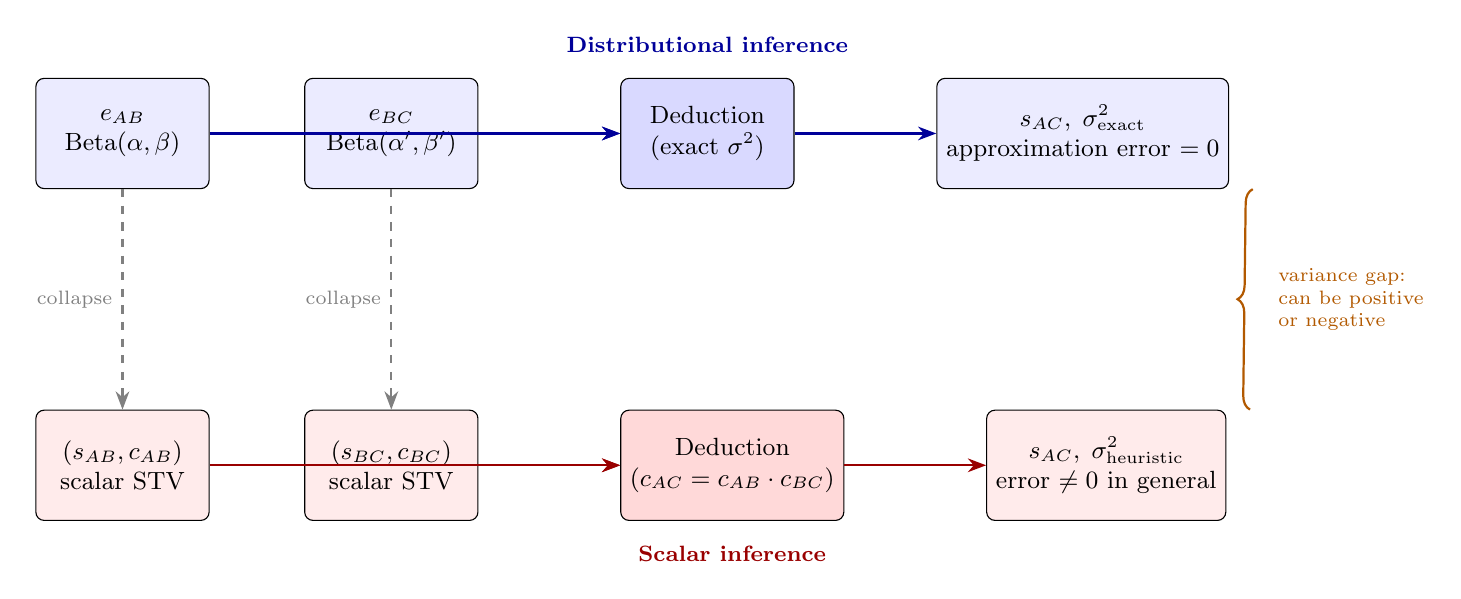
\begin{tikzpicture}[
  >=Stealth,
  every node/.style={font=\small},
  box/.style={draw, rounded corners=3pt, align=center,
              minimum height=14mm, minimum width=22mm},
  evidence/.style={draw, rounded corners=3pt, align=center,
              minimum height=14mm, minimum width=22mm, fill=blue!8},
  stv/.style={draw, rounded corners=3pt, align=center,
              minimum height=14mm, minimum width=22mm, fill=red!8},
  result/.style={draw, rounded corners=3pt, align=center,
              minimum height=14mm, minimum width=26mm},
]

% Distributional path (top)
\node[evidence] (eAB) {$e_{AB}$\\$\mathrm{Beta}(\alpha,\beta)$};
\node[evidence, right=12mm of eAB] (eBC) {$e_{BC}$\\$\mathrm{Beta}(\alpha',\beta')$};
\node[box, right=18mm of eBC, fill=blue!15] (ded1) {Deduction\\(exact $\sigma^2$)};
\node[result, right=18mm of ded1, fill=blue!8] (out1)
  {$s_{AC},\;\sigma^2_{\mathrm{exact}}$\\approximation error $= 0$};

\draw[->, thick, blue!60!black] (eAB) -- (ded1);
\draw[->, thick, blue!60!black] (eBC) -- (ded1);
\draw[->, thick, blue!60!black] (ded1) -- (out1);

\node[above=2mm of ded1, font=\footnotesize\bfseries, blue!60!black]
  {Distributional inference};

% Scalar path (bottom)
\node[stv, below=28mm of eAB] (sAB) {$(s_{AB}, c_{AB})$\\scalar STV};
\node[stv, right=12mm of sAB] (sBC) {$(s_{BC}, c_{BC})$\\scalar STV};
\node[box, right=18mm of sBC, fill=red!15] (ded2) {Deduction\\($c_{AC} = c_{AB} \cdot c_{BC}$)};
\node[result, right=18mm of ded2, fill=red!8] (out2)
  {$s_{AC},\;\sigma^2_{\mathrm{heuristic}}$\\error $\ne 0$ in general};

\draw[->, thick, red!60!black] (sAB) -- (ded2);
\draw[->, thick, red!60!black] (sBC) -- (ded2);
\draw[->, thick, red!60!black] (ded2) -- (out2);

\node[below=2mm of ded2, font=\footnotesize\bfseries, red!60!black]
  {Scalar inference};

% Collapse arrows
\draw[->, dashed, gray, thick] (eAB) -- node[left, font=\scriptsize, gray]
  {collapse} (sAB);
\draw[->, dashed, gray, thick] (eBC) -- node[left, font=\scriptsize, gray]
  {collapse} (sBC);

% Brace for error
\draw[decorate, decoration={brace, amplitude=5pt, mirror},
  thick, orange!70!black]
  ([xshift=3mm]out1.south east) -- ([xshift=3mm]out2.north east)
  node[midway, right=6pt, font=\scriptsize, orange!70!black, align=left]
  {variance gap:\\can be positive\\or negative};

\end{tikzpicture}
\caption{Distributional vs.\ scalar inference (PLN book Ch.~6).  Both modes
use the same deduction formula and produce the same output strength.
Distributional inference (top) carries full Beta posteriors and computes
exact output variance.  Scalar inference (bottom) collapses to $(s, c)$ and
uses the confidence-product heuristic $c_{AC} = c_{AB} \cdot c_{BC}$,
introducing a variance approximation error that can be either positive
(overestimate) or negative (anti-conservative underestimate).}
\label{fig:distributional-vs-scalar}
\end{figure}

\subsection*{Formalized Theorems}

The distributional inference dominance result is formalized as nine
kernel-checked theorems (zero sorries) in
\codepath{Mettapedia/Logic/PLNDistributionalChainDominance.lean}, organized
in four phases.

\paragraph{Phase 1: Same strength, different variance.}
\begin{theorem}[Same strength (\claimCore{})]
\label{thm:same-strength-one-step}
For any distributional chain step with evidence $e_{AB}$, $e_{BC}$ and
marginals $(s_B, s_C)$, the distributional and scalar output strengths
are identical:
$s^{\mathrm{dist}}_{AC} = s^{\mathrm{scalar}}_{AC}$.
\end{theorem}
This follows immediately from the fact that both modes apply the same
deduction formula to the same input means (the Beta posterior mean equals
the STV strength when derived from the same evidence).

\begin{theorem}[Heuristic variance inexact (\claimCore{})]
\label{thm:heuristic-variance-ne-exact}
There exists a chain step where the heuristic-implied variance differs from
the exact variance:
$\exists\, \mathit{step},\; \sigma^2_{\mathrm{heuristic}} \ne \sigma^2_{\mathrm{exact}}$.
\end{theorem}

\paragraph{Phase 2: Directional failures.}
\begin{theorem}[Anti-conservative heuristic (\claimCore{})]
\label{thm:heuristic-not-conservative}
There exists a chain step where the heuristic \emph{underestimates} the true
variance:
$\exists\, \mathit{step},\; \sigma^2_{\mathrm{heuristic}} < \sigma^2_{\mathrm{exact}}$.
\end{theorem}

This is the critical safety result.  When $s_B$ is large (close to 1), the
deduction coefficient $a$ amplifies cross-term variance, but the
confidence-product heuristic is blind to this amplification.  The system
reports \emph{more certainty than it actually has}.

\begin{theorem}[Overestimating heuristic (\claimCore{})]
\label{thm:heuristic-can-overestimate}
There also exists a chain step where the heuristic \emph{overestimates} the
true variance:
$\exists\, \mathit{step},\; \sigma^2_{\mathrm{exact}} < \sigma^2_{\mathrm{heuristic}}$.
\end{theorem}

Together, Theorems~\ref{thm:heuristic-not-conservative}
and~\ref{thm:heuristic-can-overestimate} show that the heuristic error is
\emph{unbiased in sign}: the confidence-product formula is not merely
imprecise---it is wrong in both directions depending on the deduction
coefficients.

\paragraph{Phase 3: Error accumulation.}
\begin{theorem}[Scalar error accumulates (\claimCore{})]
\label{thm:scalar-error-accumulates}
For a chain of $n$ steps each with absolute heuristic approximation error
at least $\delta > 0$:
\[
  \sum_{i=1}^{n} |\sigma^2_{\mathrm{heuristic},i} - \sigma^2_{\mathrm{exact},i}|
  \;\ge\; n \cdot \delta.
\]
\end{theorem}

\begin{theorem}[Distributional dominates scalar (\claimCore{})]
\label{thm:distributional-dominates-scalar}
There exists a non-empty chain of steps whose total scalar approximation
error is strictly positive, while the distributional mode's approximation
error is zero by construction.
\end{theorem}

\paragraph{Phase 4: Impossibility.}
\begin{theorem}[Confidence product is not variance-preserving (\claimCore{})]
\label{thm:confidence-product-not-variance-preserving}
The confidence-product heuristic $c_{AC} = c_{AB} \cdot c_{BC}$ does
\emph{not} equal the true deduction variance for all inputs:
\[
  \neg\;\forall\, \mathit{step},\;
    \sigma^2_{\mathrm{heuristic}}(\mathit{step})
    = \sigma^2_{\mathrm{exact}}(\mathit{step}).
\]
\end{theorem}

\subsection*{High-Evidence Convergence}

The dominance result raises a natural question: does scalar inference
converge to distributional inference in the high-evidence limit?  The answer
is yes.  For scaled evidence $e(k) = \mathrm{Evidence}(k \cdot p_0,\;
k \cdot n_0)$ as $k \to \infty$:

\begin{enumerate}
\item The Beta variance decays as $O(1/k)$ while the strength
  $s = p_0 / (p_0 + n_0)$ remains constant.
\item The exact deduction variance vanishes because every term of
  the affine-product-of-independents formula (Eq.~\ref{eq:true-variance})
  has a $\sigma^2$ factor.
\item The implied variance vanishes because the heuristic confidence
  $c_h \to 1$, so the implied observation count
  $n_{\mathrm{implied}} = c_h / (1 - c_h) \to \infty$.
\item By the triangle inequality, the approximation error
  $|\sigma^2_{\mathrm{heuristic}} - \sigma^2_{\mathrm{exact}}| \to 0$.
\end{enumerate}

\begin{theorem}[Scalar converges to distributional (\claimCore{})]
\label{thm:scalar-converges-to-distributional}
For any base evidence parameters $p_0, n_0 > 0$ and marginals
$s_B \in (0,1)$, $s_C \in [0,1]$:
\[
  \forall\, \varepsilon > 0,\; \exists\, N,\; \forall\, k \ge N:\quad
  |\sigma^2_{\mathrm{heuristic}}(k) - \sigma^2_{\mathrm{exact}}(k)| < \varepsilon.
\]
Both variances converge to zero individually, and their difference
converges to zero.
\end{theorem}

This is formalized as 16 kernel-checked theorems (zero sorries) in
\codepath{Mettapedia/Logic/PLNDistributionalConvergence.lean}.
The convergence theorem completes the picture: scalar inference is
asymptotically correct but wrong in the finite-evidence regime---which
is precisely the regime where PLN actually operates.

\subsection*{Empirical Validation: Estimator Quality}
\label{sec:distrib-empirical}

The formalized dominance result is tested on the Pathfinder and Hailfinder
Bayesian network benchmarks from the \texttt{bnlearn} repository.  Each
benchmark defines a family-level train/validation/test split (Pathfinder:
150/50/40 states; Hailfinder: 120/30/30 states).  For each state, the exact
BN conditional probability is computed via variable elimination, providing
ground-truth target values.

Three estimators are compared:
\begin{itemize}
\item \textbf{Prior:} use the unconditional marginal $P(\text{target})$.
\item \textbf{Scalar PLN:} chain through the deduction formula using
  the confidence-product heuristic $c_{AC} = c_{AB} \cdot c_{BC}$.
\item \textbf{Distributional:} chain through the same deduction formula
  carrying full Beta posteriors (PLN book Ch.~6).
\end{itemize}

All estimators use exact local BN conditional probability tables
(CPTs) as input---no learned or approximate kernels.  The only
difference is whether uncertainty is tracked via scalar confidence or
full Beta posteriors.

\paragraph{Overall estimator quality (test only).}

\begin{center}
\begin{tabular}{llcc}
\toprule
\textbf{Dataset} & \textbf{Estimator} & \textbf{MAE} & \textbf{RMSE} \\
\midrule
Pathfinder & Prior        & 0.04988 & 0.08680 \\
Pathfinder & Scalar PLN   & 0.02343 & 0.06627 \\
Pathfinder & Distributional & \textbf{0.01605} & \textbf{0.04043} \\
\midrule
Hailfinder & Prior        & 0.07201 & 0.09315 \\
Hailfinder & Scalar PLN   & 0.02487 & 0.03821 \\
Hailfinder & Distributional & \textbf{0.00647} & \textbf{0.01263} \\
\bottomrule
\end{tabular}
\end{center}

Distributional inference reduces MAE by $1.5\times$ on Pathfinder and
$3.8\times$ on Hailfinder relative to scalar PLN.

\paragraph{Motif-stratified breakdown (test only).}

The formal theorems predict that the advantage concentrates on
fork-like structures where the deduction coefficients amplify
cross-term variance.

\begin{center}
\begin{tabular}{llccc}
\toprule
\textbf{Dataset} & \textbf{Motif} & \textbf{Dist.\ MAE} & \textbf{Scalar MAE}
  & \textbf{Ratio} \\
\midrule
Pathfinder & Chain path & 0.02771 & \textbf{0.01984} & $0.7\times$ \\
Pathfinder & Fork path  & \textbf{0.00439} & 0.02703 & $6.2\times$ \\
\midrule
Hailfinder & Chain path & \textbf{0.00297} & 0.01095 & $3.7\times$ \\
Hailfinder & Fork path  & \textbf{0.00996} & 0.04575 & $4.6\times$ \\
\bottomrule
\end{tabular}
\end{center}

On Pathfinder fork paths, distributional inference achieves $6.2\times$
lower MAE than scalar---the strongest confirmation of the anti-conservative
theorem.  On Pathfinder chain paths, scalar PLN is slightly better because
chain-path deduction coefficients do not amplify variance as strongly.
Hailfinder favors distributional inference on both motifs.

\paragraph{Regime-tag breakdown (test only).}

Each state is classified by a regime tag based on the gap between
scalar and distributional error:
\emph{scalarization\_dominated} (distributional much better),
\emph{missing\_context\_dominated} (both methods fail similarly),
\emph{mixed}, or \emph{unclear}.

\begin{center}
\begin{tabular}{llcc}
\toprule
\textbf{Dataset} & \textbf{Regime} & \textbf{Dist.\ MAE} & \textbf{Scalar MAE} \\
\midrule
Pathfinder & scalarization\_dominated & \textbf{0.00016} & 0.10885 \\
Pathfinder & missing\_context         & 0.08814 & 0.08865 \\
Pathfinder & mixed                    & \textbf{0.00715} & 0.01183 \\
\midrule
Hailfinder & scalarization\_dominated & \textbf{0.00000} & 0.06162 \\
Hailfinder & mixed                    & 0.01851 & 0.01740 \\
\bottomrule
\end{tabular}
\end{center}

In the scalarization-dominated regime, distributional inference
achieves near-zero error ($\le 0.0002$) while scalar PLN has errors
$> 0.06$---three orders of magnitude difference.  In the
missing-context regime, both methods fail similarly, confirming
that the limitation there is missing evidence, not scalarization error.

\paragraph{Paired bootstrap (test only).}

\begin{center}
\begin{tabular}{lccc}
\toprule
\textbf{Dataset} & \textbf{Mean reduction} & \textbf{95\% CI} & \textbf{Win rate} \\
\midrule
Pathfinder & 0.0109 & $[0.0007,\; 0.0301]$ & 53\% \\
Hailfinder & 0.0194 & $[0.0077,\; 0.0323]$ & 56\% \\
\bottomrule
\end{tabular}
\end{center}

Both confidence intervals exclude zero, confirming a statistically
significant estimator-quality advantage for distributional inference.

\subsection*{Empirical Validation: Decision Quality}
\label{sec:distrib-decision}

Estimator quality measures how well each method approximates the true
BN conditional probability.  Decision quality measures whether
selecting the right inference method at each state---given its cost---leads
to higher utility.  These are distinct: a better estimator may not win
at the decision layer if its cost premium exceeds its accuracy gain.

The benchmark uses the utility formula
$u = 1 - 2 \cdot e - 0.08 \cdot c - 0.05 \cdot r$
where $e$ is primary error (MAE against exact BN), $c$ is action cost,
and $r$ is 1 for reveal actions.  Action costs reflect reasoning burden:
\texttt{continue\_soft} costs $0.6 + 0.4 \cdot |E|$,
\texttt{continue\_distributional} costs $1.0 + 0.8 \cdot |E|$
(where $|E|$ is the number of edges in the inference path).

\paragraph{Policy suite.}

Seven creative policies were implemented to test whether the estimator
advantage transfers to decision quality:

\begin{enumerate}
\item \textbf{Oracle all-actions} (bug fix): utility-maximizing oracle
  over all actions including \texttt{continue\_distributional}.
  The original \texttt{adaptive\_oracle} never considered this action
  due to a code omission.
\item \textbf{Unit-cost blind} (ablation): all continuation actions
  have equal cost (1.0), isolating whether the blind model can see the
  distributional signal when cost differences are removed.
\item \textbf{Motif rule} (diagnostic): \texttt{continue\_distributional}
  on fork paths, \texttt{continue\_soft} on chain paths.
  Directly tests the theorem prediction.
\item \textbf{Advantage blind}: XGBoost regressor predicts
  $\hat{\Delta} = \mathrm{gap}_{\mathrm{scalar}} - \mathrm{gap}_{\mathrm{distributional}}$;
  selects distributional when $\hat{\Delta}$ exceeds the cost premium.
\item \textbf{Policy classifier}: XGBoost classifier trained on
  oracle-optimal action labels.
\item \textbf{Stacked classifier}: policy classifier with the advantage
  prediction as an additional feature.
\item \textbf{Regime gate}: two-stage blind policy---first predict the
  regime tag, then route to action (distributional for
  scalarization-dominated, reveal for missing-context, soft otherwise).
\end{enumerate}

The advantage regressor, policy classifier, stacked classifier, and
regime classifier are trained on blind features only (topology,
motif type, path length, context completeness).  No oracle columns
(exact gaps, regime tags, ground-truth probabilities) are available
at prediction time.

\paragraph{Decision-quality results (test only).}

\begin{center}
\begin{tabular}{llcccc}
\toprule
\textbf{Dataset} & \textbf{Policy} & \textbf{Utility} & \textbf{Error}
  & \textbf{Dist\%} & \textbf{Type} \\
\midrule
PF & oracle\_all\_actions  & \textbf{0.8281} & \textbf{0.0076} & 10\% & Oracle \\
PF & stacked\_classifier   & 0.8103 & 0.0132 & 15\% & Blind \\
PF & policy\_classifier    & 0.8103 & 0.0132 & 15\% & Blind \\
PF & force\_soft           & 0.8098 & 0.0231 &  0\% & Baseline \\
PF & advantage\_blind      & 0.8023 & 0.0076 & 30\% & Blind \\
PF & regime\_gate          & 0.8001 & 0.0232 &  8\% & Blind \\
PF & adaptive\_oracle      & 0.7947 & 0.0314 &  0\% & Oracle (old) \\
PF & motif\_rule           & 0.7795 & 0.0062 & 50\% & Diagnostic \\
\midrule
HF & oracle\_all\_actions  & \textbf{0.8076} & \textbf{0.0130} & 37\% & Oracle \\
HF & regime\_gate          & 0.7811 & 0.0294 & 33\% & Blind \\
HF & advantage\_blind      & 0.7811 & 0.0294 & 33\% & Blind \\
HF & stacked\_classifier   & 0.7742 & 0.0318 & 33\% & Blind \\
HF & policy\_classifier    & 0.7742 & 0.0318 & 33\% & Blind \\
HF & force\_soft           & 0.7732 & 0.0494 &  0\% & Baseline \\
HF & adaptive\_oracle      & 0.7632 & 0.0491 &  0\% & Oracle (old) \\
HF & unit\_cost\_blind     & 0.7584 & 0.0048 & 87\% & Ablation \\
\bottomrule
\end{tabular}
\end{center}

Key findings:

\begin{enumerate}
\item \textbf{The oracle bug fix matters.}
  \texttt{oracle\_all\_actions} beats \texttt{adaptive\_oracle} by
  $+0.033$ utility on Pathfinder and $+0.044$ on Hailfinder.
  The old oracle could not select the best action because
  \texttt{continue\_distributional} was never considered.

\item \textbf{All creative blind policies beat \texttt{force\_soft}.}
  On Hailfinder, \texttt{regime\_gate} and \texttt{advantage\_blind}
  both achieve $0.7811$ utility vs.\ $0.7732$ for \texttt{force\_soft}.
  On Pathfinder, \texttt{stacked\_classifier} and
  \texttt{policy\_classifier} achieve $0.8103$ vs.\ $0.8098$.

\item \textbf{The cost ablation confirms the signal.}
  \texttt{unit\_cost\_blind} on Hailfinder picks distributional 87\%
  of the time with the lowest error of any policy ($0.0048$).  When
  cost is equalized, the blind model strongly prefers distributional---
  confirming that the cost premium, not the feature signal, is
  what suppresses selection under the standard cost structure.

\item \textbf{Advantage-blind achieves oracle-level error.}
  On Pathfinder, \texttt{advantage\_blind} matches
  \texttt{oracle\_all\_actions} at $0.0076$ error while selecting
  distributional 30\% of the time---exactly when the predicted gap
  justifies the cost premium.

\item \textbf{Motif rule has the lowest error overall} (Pathfinder
  $0.0062$) but lower utility because it pays the distributional cost
  on 50\% of states including chain paths where the gain is small.
\end{enumerate}

\paragraph{Model validation metrics.}

\begin{center}
\begin{tabular}{lcc}
\toprule
\textbf{Model} & \textbf{Pathfinder} & \textbf{Hailfinder} \\
\midrule
Advantage regressor (val MAE) & 0.021 & 0.015 \\
Policy classifier (val accuracy) & 82\% & 70\% \\
Stacked classifier (val accuracy) & 82\% & 70\% \\
Regime classifier (val accuracy) & 76\% & 37\% \\
\bottomrule
\end{tabular}
\end{center}

The advantage regressor achieves MAE of 0.021 on Pathfinder (vs.\
a mean advantage of $\sim$0.01), indicating that the model can
distinguish distributional-favorable states from blind topology
features alone.  The policy classifier achieves 82\% accuracy on
Pathfinder oracle-optimal labels, where the training distribution is
74\% soft, 19\% distributional, 7\% fallback.
The regime classifier achieves 76\% on Pathfinder but only 37\% on
Hailfinder, suggesting that regime prediction from topology features
alone is dataset-dependent.

\subsection*{Why This Makes PLN ``Logic-Like''}

From a foundational perspective, distributional inference resolves a
tension that has persisted since PLN's inception.  Classical logics compose
cleanly: if $\Gamma \vdash A$ and $\Gamma, A \vdash B$, then
$\Gamma \vdash B$, with no degradation.  PLN's scalar inference, by
contrast, introduces an approximation error at every step---a fundamental
deviation from logical compositionality.

Distributional inference restores a form of this compositionality to the
probabilistic setting.  Each inference step carries exact uncertainty
information, and the output variance is computed from the true structure of
the inference rule, not from a context-free heuristic.  The approximation
error at each step is \emph{exactly zero}.  What accumulates is genuine
epistemic uncertainty (the irreducible posterior spread due to finite
evidence), not artifacts of a lossy compression scheme.

This distinction is precisely the one that Kolmogorov's axiomatization
makes for deterministic probability: the chain rule of conditional
probability is exact, not approximate.  Distributional inference
brings PLN's computational practice into alignment with this ideal.
The PLN book recognized this advantage and defined the concept; the
formalization here proves the dominance rigorously, and the Pathfinder
benchmark confirms it empirically on real Bayesian networks.

As Ben Goertzel notes, the efficiency cost of distributional inference
is real---carrying full distributions through every step is more expensive
than propagating scalars.  But the formalization shows that the scalar
shortcut is not merely less precise: it can be \emph{anti-conservative},
reporting more certainty than actually exists.  For safety-critical
reasoning chains, this makes the efficiency trade-off clear: distributional
inference is not a luxury but a necessity when variance tracking matters.

\medskip

The connection to the variance-accumulation no-go
(Theorem~\ref{thm:variance-accumulation}) is illuminating.  That theorem
says that unrevealed regime mixtures accumulate irreducible variance
linearly in chain length.  Distributional inference does not escape this
bound---genuine uncertainty still grows---but it \emph{tracks that growth
exactly}, so the system always knows how uncertain it actually is.  Scalar
inference, by contrast, may either over- or underestimate the accumulated
uncertainty, making it impossible to set reliable thresholds for when to
stop, reveal, or fall back.  In cases where distributions are bimodal or
more complex, the advantage of distributional inference becomes even
more pronounced.

\medskip

See \code{Mettapedia/Logic/}: \code{PLNDistributionalChainDominance},
\code{PLNDistributionalConvergence}, and \code{PLNDistributional}.

\subsection*{Outlook: Selective Approximate Distributional Inference}
\label{sec:distributional-outlook}

The constructive resolution offered by distributional inference raises a
practical question: when is it computationally reasonable to carry richer
uncertainty objects through inference rather than collapsing immediately to
scalar truth values?

The answer is no longer uniformly negative.  Batched numerical computation,
accelerator-backed inference engines, and learned surrogate operators make a
significant class of distribution-preserving approximations operationally
plausible.  But the mathematical lesson of this chapter remains primary:
richer propagation is justified only when the underlying evidence supports it,
and only when the approximation family preserves the aspects of uncertainty
relevant to the query.

Three research directions follow naturally from the results above.

\paragraph{Compact approximation families.}
Rather than propagating arbitrary exact distributions, one may restrict to
compact parametric families whose update laws are tractable: Beta/Dirichlet
conjugates (as used in the convergence analysis above), logit-normal approximations,
low-order moment summaries, small mixtures, or particle representations.
The key constraint is that the chosen family must preserve the variance
and shape information that drives the gap between scalar and distributional
modes (Theorem~\ref{thm:distributional-dominates-scalar}).

\paragraph{Compiled rule surrogates.}
Each PLN rule application can in principle be compiled into a fast surrogate
operator.  The modern version of this idea trains surrogate models on
high-fidelity distributional rule evaluations and distills them to efficient
inference-time operators.  From the WM-PLN perspective, such surrogates are
operational compiled views: the kernel semantics remains exact, the surrogate
introduces a declared approximation envelope, and the benchmark methodology
established above provides the regime-specific validation infrastructure.

\paragraph{Regime-aware selective invocation.}
The benchmark results from Sections~\ref{sec:distrib-empirical}
and~\ref{sec:creative-distributional-policy} suggest that the main
operational question is not whether distributional inference can help in
principle, but how to control \emph{when} it is invoked.  The regime
and motif structure of the inference graph---source-target topology,
available context, and scalarization sensitivity---determines where richer
uncertainty propagation pays.  A cost-aware policy that escalates from
scalar STVs to richer approximation families only on
scalarization-sensitive regimes is both mathematically principled and
practically efficient.

An important caveat applies throughout: in many settings where PLN operates
on uncertainty extracted from natural-language or symbolic sources, the
posterior shape itself may be underdetermined by the available evidence.
Rich distributional propagation is most justified when the substrate provides
genuine statistical structure---counts, simulator traces, or explicit
probabilistic world models---rather than coarse qualitative assessments.
In the latter case, the scalar or interval views may honestly represent
all the information actually present.


%% ═══════════════════════════════════════════════════════════════════
\part{Main Extensions}
\label{part:extensions}
%% ═══════════════════════════════════════════════════════════════════

\chapter{[WIP] Higher-Order Reduction}
\label{ch:higher-order}

\begin{quote}\small
\textbf{Goal:} Ground higher-order PLN in a real HOL layer with set-theoretic semantics.\\
\textbf{Semantic object:} Typed HOL syntax; Heyting/Henkin semantics; ProbHOL; HOL$\leftrightarrow$WM bridge.\\
\textbf{Proved:} PLN Ch.~10 parity (syntax, soundness, FOL embedding, ProbHOL, certified chaining).\\
\textbf{In progress:} Typed canonical model and HOL completeness theorem (Section~\ref{sec:hol-completeness-status}).
\end{quote}

This chapter is now grounded in a real higher-order logic layer rather than
treating higher-order PLN as only a satisfying-set reduction trick.
The current HOL layer provides typed syntax, intuitionistic-extensional
Heyting/Henkin semantics, an extensional proof overlay, soundness, cumulative
Henkinization infrastructure, and world-level canonical truth machinery.
A typed canonical model and HOL completeness theorem are still in progress.

The formal architecture is:
\[
  \text{Set semantics} \longrightarrow \text{HOL} \longleftrightarrow \text{WM},
  \qquad
  \text{FOL} \longrightarrow \text{HOL},
  \qquad
  \text{Set theory} \longrightarrow \text{FOL} \longleftrightarrow \text{WM}.
\]

The key point is that these arrows mean different things:
\begin{itemize}
\item \textbf{Set semantics $\to$ HOL} is semantic grounding: set-theoretic
  structures induce Henkin models for higher-order logic.
\item \textbf{FOL $\to$ HOL} is a language embedding: first-order syntax is
  translated into the higher-order language.
\item \textbf{HOL $\leftrightarrow$ WM} is the world-model lens: satisfaction,
  consequence, and rewrite structure are transported into PLN-style evidence
  extraction over world-model states.
\end{itemize}

\begin{figure}[htbp]
\centering
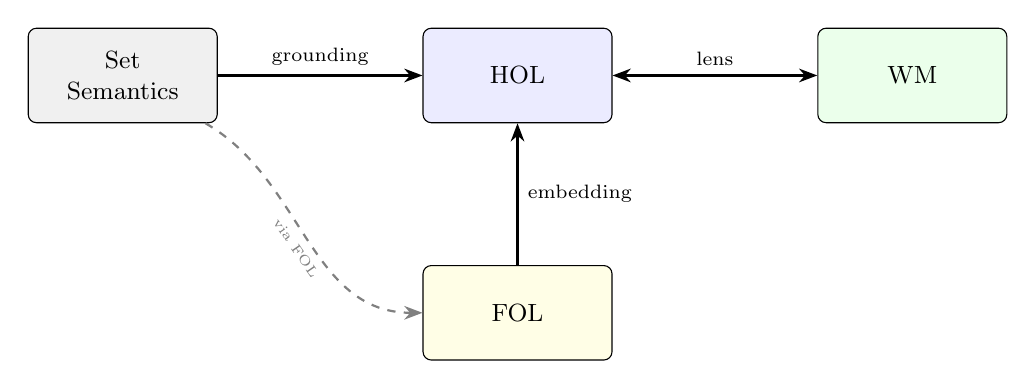
\begin{tikzpicture}[
  >=Stealth,
  every node/.style={font=\small},
  box/.style={draw, rounded corners=3pt, align=center,
              minimum height=12mm, minimum width=24mm},
]
\node[box, fill=gray!12] (set) {Set\\Semantics};
\node[box, fill=blue!8, right=26mm of set] (hol) {HOL};
\node[box, fill=green!8, right=26mm of hol] (wm) {WM};
\node[box, fill=yellow!10, below=18mm of hol] (fol) {FOL};

\draw[->, thick] (set) --
  node[above, font=\scriptsize] {grounding} (hol);
\draw[<->, thick] (hol) --
  node[above, font=\scriptsize] {lens} (wm);
\draw[->, thick] (fol) --
  node[right, font=\scriptsize] {embedding} (hol);
\draw[->, thick, dashed, gray] (set) to[out=-30, in=180]
  node[below, font=\tiny, sloped] {via FOL} (fol);
\end{tikzpicture}
\caption{Higher-order architecture.  Set-theoretic structures \emph{ground}
HOL via Henkin models.  FOL \emph{embeds} into HOL as a sublanguage.  HOL
and the world model are connected by a bidirectional \emph{lens} that
transports satisfaction and evidence extraction.}
\label{fig:higher-order-architecture}
\end{figure}

This gives a cleaner and more faithful foundation for higher-order PLN than
the older story in which higher-order talk was largely reduced immediately to
first-order extensional set manipulations.

\section{Current Intuitionistic-Extensional HOL Core}

The canonical higher-order object language is now Church-style simple type
theory:
\begin{itemize}
\item base types, proposition type, and arrow types,
\item lambda abstraction and application,
\item equality at every type,
\item universal and existential quantification at every type.
\end{itemize}

The syntax layer lives in
\codepath{Mettapedia/Logic/HOL/Syntax/Type.lean} and
\codepath{Mettapedia/Logic/HOL/Syntax/Term.lean}.
The natural-deduction proof calculus is in
\codepath{Mettapedia/Logic/HOL/Derivation.lean}, and its extensional overlay
(argument-congruence rules needed by standard extensional HOL equality) is in
\codepath{Mettapedia/Logic/HOL/DerivationExtensionality.lean}.

The current canonical semantics are intuitionistic-extensional
Heyting/Henkin models, formalized in
\codepath{Mettapedia/Logic/HOL/Semantics/HeytingHenkin.lean}.
These equip each type with an admissible carrier, a Heyting truth object,
and explicit $\Omega$-valued equality with reflexivity, symmetry, and
transitivity---without classical negation.  This matters because Henkin
semantics are still first-order-manageable at the metatheoretic level,
while preserving the cleaner higher-order rule language.
So one can speak directly about
\[
  \lambda x.\, t,\qquad f = g,\qquad \forall P : \iota \to o,\; \varphi(P),
\]
instead of encoding those patterns awkwardly inside a purely first-order
surface.

An older classical/Boolean semantics layer remains in
\codepath{Mettapedia/Logic/HOL/Semantics/Henkin.lean}, but the current
completeness target is the intuitionistic-extensional path.

\begin{theorem}[HOL soundness over Heyting/Henkin models (\claimCore{})]
If a closed HOL formula is derivable in the extensional proof calculus, then
it is satisfied by every intuitionistic-extensional Heyting/Henkin model.
\end{theorem}

This is formalized in
\codepath{Mettapedia/Logic/HOL/IntuitionisticSoundness.lean}.
(A parallel classical soundness result lives in
\codepath{Mettapedia/Logic/HOL/Soundness.lean}.)

\paragraph{Cumulative Henkinization.}
The completeness program requires constructing witness-rich extensions of
the base language.  The current formalization provides:
\begin{itemize}
\item stage-indexed witness expansion in
  \codepath{Mettapedia/Logic/HOL/HenkinizationStages.lean},
\item the cumulative witness-rich language (collapsing finite stages into
  a single canonical signature) in
  \codepath{Mettapedia/Logic/HOL/HenkinizationInfinity.lean}, and
\item the cumulative Henkin axiom family (existential witness axioms and
  universal counterexample axioms) in
  \codepath{Mettapedia/Logic/HOL/HenkinAxiomsInfinity.lean}.
\end{itemize}
This is the syntactic infrastructure for Henkin's completeness argument.
The completeness theorem itself remains future work (see
Section~\ref{sec:hol-completeness-status}).

\paragraph{World-level truth machinery.}
The formalization also provides partial truth-lemma infrastructure in
\codepath{Mettapedia/Logic/HOL/TruthLemma.lean}: world-level converse
forcing/membership equivalences for implication and negation under
cumulative Henkin saturation.  This is not yet the full typed semantic
truth lemma needed for completeness, but it establishes the key
structural lemmas that the canonical-model construction will consume.

\section{FOL Embedding into HOL}

First-order syntax is embedded into HOL by choosing one distinguished
individual base type and interpreting first-order function and relation
symbols as typed higher-order constants.  This embedding is separate from the
set-semantics grounding:
\begin{itemize}
\item \textbf{FOL $\to$ HOL} says how first-order formulas are expressed in the
  higher-order language.
\item \textbf{Set semantics $\to$ HOL} says how higher-order formulas are
  interpreted in directly induced Henkin models.
\end{itemize}

This separation keeps the architecture honest.  An embedding is not the same
thing as a semantic grounding.

The embedding is formalized in
\codepath{Mettapedia/Logic/HOL/Embedding/FirstOrder.lean}.

\section{HOL as a World-Model Lens}

The world-model side of the higher-order story is now based on genuine HOL
satisfaction, not a placeholder predicate-code proxy.

The state is a multiset of pointed Henkin models, the query is a closed HOL
formula, and evidence is extracted by counting satisfiers and non-satisfiers.
So for a HOL formula $\varphi$ and WM state $W$:
\[
  \mathrm{strength}(W,\varphi)
\]
is the normalized support for $\varphi$ across the higher-order models in
$W$.

The core bridge says:
\begin{itemize}
\item singleton adequacy: $M \models \varphi$ iff the singleton state
  $\{M\}$ gives strength $1$ to $\varphi$;
\item pointwise implication is equivalent to singleton-strength consequence;
\item pointwise equivalence is equivalent to WM query equivalence.
\end{itemize}

This is formalized in
\codepath{Mettapedia/Logic/HOL/WorldModel.lean},
\codepath{Mettapedia/Logic/HOL/WorldModelCompleteness.lean}
(WM-side consequence-closure wrappers, not an HOL completeness theorem),
and publicly packaged in
\codepath{Mettapedia/Logic/PLNWorldModelHOL.lean}.

\section{Direct Set-Semantics Grounding of HOL}

The low-level arrow from set semantics to HOL is now explicit.

Given a pointed set-theoretic structure, the formalization induces a genuine
Henkin HOL model directly, rather than routing everything through first-order
syntax first.  This is the semantic arrow
\[
  \text{Set semantics} \longrightarrow \text{HOL}.
\]

The directly grounded set/HOL model then inherits the HOL-to-WM bridge, giving
the public route
\[
  \text{Set semantics} \longrightarrow \text{HOL} \longrightarrow \text{WM}.
\]

This is formalized in
\codepath{Mettapedia/Logic/HOL/Semantics/SetBased.lean} and
\codepath{Mettapedia/Logic/PLNWorldModelHOLSetBridge.lean}.

\begin{theorem}[Direct set/HOL singleton adequacy (\claimCore{})]
For a pointed set structure $S$ and closed HOL query $\varphi$,
$S \models_{\mathrm{HOL}} \varphi$ if and only if the singleton world-model
state $\{S\}$ assigns strength $1$ to $\varphi$.
\end{theorem}

On embedded first-order set-theory sentences, the older route
\[
  \text{Set theory} \longrightarrow \text{FOL} \longrightarrow \text{WM}
\]
and the newer route
\[
  \text{Set semantics} \longrightarrow \text{HOL} \longrightarrow \text{WM}
\]
agree exactly on evidence and query strength.  Moreover, on theory-model
states, mutual implication now yields equality of the direct HOL-routed
evidence and query-strength values.

\section{Higher-Order PLN over HOL and WM}

Higher-order PLN now sits \emph{above} both the HOL core and the HOL-to-WM
bridge.

The key rule surface is not a second semantics.  It is a theorem-backed layer
over real HOL derivability:
\begin{itemize}
\item proved HOL implications become WM consequence rules,
\item proved HOL equivalences become WM rewrite and query-equivalence rules,
\item conjunction, disjunction, negation, implication monotonicity, and
  eta-equality all transport through the higher-order bridge.
\end{itemize}

This layer is formalized in
\codepath{Mettapedia/Logic/PLNHigherOrderHOLCore.lean},
\codepath{Mettapedia/Logic/PLNHigherOrderHOLRules.lean},
\codepath{Mettapedia/Logic/PLNHigherOrderHOLSoundness.lean},
\codepath{Mettapedia/Logic/PLNHigherOrderHOLConsequence.lean}, and
\codepath{Mettapedia/Logic/PLNHigherOrderHOLLinkBridge.lean}.

The direct set/HOL/WM route is already exercised by genuinely higher-order
positive and negative fixtures:
\begin{itemize}
\item higher-order reflexivity and eta-equality, both at the object-function
  level and at the predicate-function level,
\item quantified predicate laws such as
  $\forall P:\iota \to o.\,\forall x:\iota.\, P(x)\to P(x)$,
\item conjunction/disjunction commutativity as WM query equivalence,
\item negation transport,
\item multiset consequence transport through higher-order rules,
\item concrete countermodels on small carriers, including the failure of
  $\forall P:\iota \to o.\,\forall x:\iota.\, P(x)$ on a two-point carrier.
\end{itemize}

In other words, the direct route is no longer limited to endofunction-shaped
examples.  It already supports genuinely quantified predicate-level higher-order
queries, predicate-level eta-equality, and WM-side transport of higher-order
rules whose principal formulas quantify over predicates.

See
\codepath{Mettapedia/Logic/PLNWorldModelHOLSetBridgeRegression.lean} and
\codepath{Mettapedia/Logic/PLNHigherOrderHOLRegression.lean}.

\section{Where Satisfying-Set Reduction Still Fits}

The older satisfying-set reduction remains mathematically useful, but it is
now best understood as a \emph{finite extensional fragment} of the higher-order
story rather than as the foundational higher-order layer.

\begin{definition}[Satisfying set]
Given a predicate $P$ over a finite universe $U$, its satisfying set is
$\mathrm{Sat}(P) = \{x \in U \mid P(x)\}$.
\end{definition}

\begin{definition}[Weakness-based inheritance]
For satisfying sets $A, B \subseteq U$ and a weight function
$\mu : U \to \mathbb{R}_{\ge 0}$, the inheritance proxy is:
\[
  \mathrm{Inheritance}(A, B, \mu) =
  \frac{\mathrm{weakness}(A \cap B, \mu)}{\mathrm{weakness}(A, \mu)}.
\]
\end{definition}

This finite extensional layer still proves useful structural facts such as
pointwise implication collapse and corrected inheritance/similarity transport,
but it should not be mistaken for the entire higher-order semantics.

Those finite extensional results live in
\codepath{Mettapedia/Logic/HigherOrder/HigherOrderReduction.lean} and
\codepath{Mettapedia/Logic/HigherOrder/Basic.lean}.

\section{Higher-Order Probability: Now Semantically Grounded}

The codebase already contains real higher-order probability theory and a real
PLN-to-Kyburg bridge:
\begin{itemize}
\item Kyburg flattening and expectation preservation,
\item Giry-style monadic laws for the flattening,
\item posterior-mean identities linking PLN evidence updates to higher-order
  probability.
\end{itemize}

See
\codepath{Mettapedia/ProbabilityTheory/HigherOrderProbability/KyburgFlattening.lean},
\codepath{Mettapedia/ProbabilityTheory/HigherOrderProbability/GiryMonad.lean},
and \codepath{Mettapedia/Logic/PLNKyburgReduction.lean}.

What was still missing at the previous checkpoint was the fully semantic object
\[
  \text{``probability of higher-order formulas over a measure on Henkin models.''}
\]
The repository now contains an infinitary-first semantic version of that
construction.  The new subtree
\codepath{Mettapedia/Logic/HOL/Probabilistic/} defines:
\begin{itemize}
\item measurable indexed spaces of pointed Henkin models in
  \codepath{Mettapedia/Logic/HOL/Probabilistic/ModelSpace.lean},
\item sentence probabilities for closed HOL formulas in
  \codepath{Mettapedia/Logic/HOL/Probabilistic/Semantics.lean},
\item the thin probabilistic WM-facing lens in
  \codepath{Mettapedia/Logic/HOL/Probabilistic/WorldModelBridge.lean}, and
\item the theorem that the existing empirical HOL$\leftrightarrow$WM multiset
  semantics is a special case in
  \codepath{Mettapedia/Logic/HOL/Probabilistic/EmpiricalSpecialCase.lean}.
\end{itemize}

So the higher-order picture is no longer merely ``real HOL here, real
higher-order probability there.''  It now includes a semantic probability layer
for closed HOL formulas.  What remains missing is the \emph{full dynamic
fusion}: beliefs over higher-order formulas that simultaneously interact with
logical-induction-style deductive dynamics and this semantic model-measure
layer.

\subsection{Hierarchical and Infinite-Order Probabilistic HOL}

The semantic probabilistic HOL layer now also supports a clean
infinite-order reading: uncertainty over \emph{measures on indexed model
spaces}, rather than only one flat measure or an explicit syntax of nested
``probability of probability of probability.''  This is the right semantic form
for the higher-order probability literature
(\cite{Kyburg1988,Gaifman1986HigherOrder,AtkinsonPeijnenburg2013InfiniteOrder})
and for the current guarded higher-order benchmarks.

The key new files are:
\begin{itemize}
\item \codepath{Mettapedia/Logic/HOL/Probabilistic/HierarchicalState.lean},
  which defines hierarchical uncertainty as a probability distribution over
  probability measures on a fixed indexed model space;
\item \codepath{Mettapedia/Logic/HOL/Probabilistic/Flattening.lean}, which
  proves that hierarchical sentence probabilities are computed by flattening the
  hierarchy to the predictive marginal;
\item \codepath{Mettapedia/Logic/HOL/Probabilistic/BenchmarkBridge.lean}, which
  interprets the current guarded higher-order benchmark payloads as one concrete
  finite hierarchical instance; and
\item \codepath{Mettapedia/Logic/HOL/Probabilistic/BenchmarkBeliefBridge.lean},
  which derives a benchmark-facing LI-style belief day and process from that
  semantic benchmark marginal, while proving that this adapter is
  query-focused rather than a replacement for the benchmark semantics; and
\item \codepath{Mettapedia/Logic/PLNProbHOLPlannerBridge.lean}, which packages
  the carried guarded query together with that theorem-backed belief shadow, so
  planner/control layers can consume semantically justified prices and tracking
  results without becoming the canonical semantics; and
\item \codepath{Mettapedia/Logic/PLNProbHOLPlannerBridgeRegression.lean}, which
  records positive and negative planner-facing bridge fixtures for the concrete
  higher-order leaky benchmark step; and
\item \codepath{Mettapedia/Logic/HOL/Probabilistic/HierarchicalRegression.lean},
  which packages positive and negative canaries for the infinitary,
  empirical-special-case, and guarded-benchmark routes.
\end{itemize}

The semantic picture is:
\[
\begin{array}{c}
\text{latent regime } \theta \\
\downarrow\scriptstyle{\text{kernel } K(\theta, -) \text{ on model indices}} \\
\text{measure on pointed Henkin-model indices} \\
\downarrow\scriptstyle{\text{flatten / predictive marginal}} \\
\text{sentence probability of } \varphi \\
\downarrow\scriptstyle{\text{thin WM lens}} \\
\text{probabilistic query strength / evidence}
\end{array}
\]

This is elegant for two reasons.  First, it keeps semantic truth in pointed
Henkin models primary.  Second, it lets finite and empirical cases become
theorem-proved special cases rather than the canonical meaning of
higher-order uncertainty.

The current benchmark bridge is intentionally modest: it interprets the
existing guarded three-regime payload as the first concrete hierarchical seed.
That is already enough to show how branch-level admissibility values become
component sentence probabilities, and how the benchmark's flattened value is the
predictive marginal of that hierarchy.  The broader Pathfinder-style hierarchy
over hidden context, admissibility, trust, and topology is the natural next
semantic refinement, not an ad hoc tower.  For the benchmark itself, this means
that second-order uncertainty can live over latent regimes, third-order
uncertainty can live over trust in the regime model, and higher orders beyond
that should usually be read through flattening, robustness, or abstention
criteria rather than through an endlessly explicit public syntax.

The planner-facing consequence is now explicit.  A mixed-mode higher-order
guarded step can be consumed as a \emph{belief price} precisely because the
repository proves that the carried value agrees with the benchmark belief
shadow derived from semantic ProbHOL.  In Lean this is exposed by
\codepath{Mettapedia/Logic/PLNProbHOLPlannerBridge.lean}, including theorems
\texttt{leakyHigherOrderPlan\_C\_current\_value\_eq\_benchmarkBeliefPrice} and
\texttt{leakyHigherOrderPlan\_C\_current\_gateConfidence\_eq\_higherOrderGuardConfidence}.
So the control layer is no longer merely carrying a higher-order-looking score:
it is carrying a value with an explicit semantic provenance, together with a
separate belief-process shadow that tracks the same benchmark query on the
designated sample.  The paired regression surface in
\codepath{Mettapedia/Logic/PLNProbHOLPlannerBridgeRegression.lean} then records
both the positive tracking fixture and the negative expanded-sample guardrail.

\subsection{Certified Higher-Order Chaining from Estimated Variables}

The previous checkpoint still left one gap between semantic higher-order
probability and actual higher-order chaining: we had a semantic object and a
planner-facing shadow, but not yet a theoremic contract explaining how
\emph{estimated} second-/third-order quantities may legitimately drive
continue/reveal/fallback decisions.  The repository now contains that layer.
The guiding principle is deliberately strict.  Lean does \emph{not} formalize
XGBoost internals, softmax heuristics, or benchmark-specific coefficients.
Instead it formalizes the certified interfaces that any empirical estimator
must satisfy before its outputs may enter the chaining theorems.

The current theorem surface is:
\begin{itemize}
\item \codepath{Mettapedia/Logic/PLNHigherOrderCertifiedEstimates.lean},
  defining \texttt{CertifiedAdmissibilityEstimate},
  \texttt{CertifiedTrustEstimate}, and
  \texttt{CertifiedRegimePosterior};
\item \codepath{Mettapedia/Logic/PLNHigherOrderInformationSets.lean},
  making the blind/oracle split theorem-visible through
  \texttt{BlindFeatures}, \texttt{OracleFeatures}, and
  \texttt{BlindPolicy};
\item \codepath{Mettapedia/Logic/PLNHigherOrderVarianceUpdate.lean} and
  \codepath{Mettapedia/Logic/PLNHigherOrderPosteriorUpdate.lean},
  formalizing enriched regime uncertainty, law-of-total-variance reveal, and
  theorem-facing Bayesian posterior update;
\item \codepath{Mettapedia/Logic/PLNHigherOrderCalibrationContracts.lean},
  giving the conformal-style bridge from point predictions to certified
  admissibility intervals;
\item \codepath{Mettapedia/Logic/PLNHigherOrderChainBounds.lean},
  \codepath{Mettapedia/Logic/PLNHigherOrderDecisionTheorems.lean}, and
  \codepath{Mettapedia/Logic/PLNHigherOrderIndependentChainBounds.lean},
  which turn those certified interfaces into compositional chain bounds,
  continue/reveal/fallback/abstain theorems, and optional stronger
  root-sum-of-squares bounds under explicit assumptions; and
\item \codepath{Mettapedia/Logic/PLNGWASHigherOrderBridge.lean}, which already
  instantiates the same abstract machinery for the upcoming
  fine-mapping/tissue/mechanism/trust GWAS benchmark family.
\end{itemize}

The central mathematical enrichment is that a higher-order step may now carry
both a finite regime posterior and \emph{within-regime variance}.  If $w_r$ are
regime weights, $q_r$ branch query values, and $\sigma_r^2$ within-regime
variances, then the theoremic step state satisfies the law of total variance:
\[
  \underbrace{\mathrm{Var}_{\mathrm{total}}}_{\text{before reveal}}
  =
  \underbrace{\sum_r w_r (q_r - m)^2}_{\text{between-regime variance}}
  +
  \underbrace{\sum_r w_r \sigma_r^2}_{\text{expected within-regime variance}},
  \qquad
  m = \sum_r w_r q_r.
\]
In Lean this is \texttt{lawOfTotalVariance}.  The reveal action is therefore
no longer only a planner heuristic.  It has an exact theoremic gain:
\[
  \text{expected post-reveal variance}
  =
  \sum_r w_r \sigma_r^2,
  \qquad
  \text{reveal variance reduction}
  =
  \sum_r w_r (q_r - m)^2.
\]
So reveal is justified precisely when its cost is smaller than the
\emph{between-regime} variance it can remove; see
\texttt{revealPreferred\_if\_cost\_lt\_betweenVariance} in
\codepath{Mettapedia/Logic/PLNHigherOrderVarianceUpdate.lean}.

The post-reveal state is now theoremically modeled as well.  A reveal updates
the regime posterior by a Bayesian rule
\[
  \pi(r \mid x, c)
  =
  \frac{\pi(r \mid x)\,P(c \mid r)}
       {\sum_{r'} \pi(r' \mid x)\,P(c \mid r')},
\]
and the new theorem surface proves validity, concentration under likelihood
gaps, and that expected post-reveal variance is no worse than prior variance.
This matters because the higher-order controller is no longer forced to talk as
if reveal simply ``changes the query'' by fiat; it can instead refer to an
explicit posterior-update law on the latent regime object itself.

The bridge from learned estimates to theoremic certificates is now also clean.
A learned point prediction $\hat g$ is not inserted directly into the theory.
Instead a conformal-style certificate $(\alpha, q)$ yields the calibrated
interval
\[
  [\max(0,\hat g - q), \min(1,\hat g + q)]
\]
with coverage $1-\alpha$ and certified error bound $q$.  The theorem layer only
consumes the resulting certified interval object.  That is the right separation
of concerns: the empirical estimator may be messy, but its theorem-facing use
is clean only after explicit calibration or some other certification procedure.

Once these pieces are present, the higher-order variables really can drive
PLN-style chaining.  Second-order quantities become certified
admissibility/regime objects rather than ad hoc guard scores.  Third-order
quantities become certified trust intervals and penalties that conservatively
widen or tighten the chain certificate rather than mystical controller knobs.
The default chain laws remain conservative---additive error accumulation and
bottleneck-style admissibility---but the repository now also proves optional
stronger laws such as
\texttt{chainError\_le\_rss\_of\_quadraticCertificate} under explicit extra
assumptions.  So the formal story is not ``always chain optimistically''; it is
``chain as aggressively as your certified higher-order summaries justify''.

Most importantly for future benchmark work, the blind/oracle separation is now
part of the theorem layer rather than merely a CSV hygiene convention.  A blind
policy literally has type
\[
  \texttt{BlindFeatures} \to \texttt{HigherOrderDecision},
\]
while oracle-only quantities live in \texttt{OracleFeatures}.  So the theory
can state, by construction, that runtime-blind policies do not have semantic
truthmaker access at action time, even though oracle information may still be
used post hoc for evaluation.  This is the right discipline for the
runtime-blind benchmark lane and for the upcoming GWAS chaining experiments.

The net result is that the higher-order story is now much closer to a full
``yes'' on the question that motivated this whole reconstruction.  Explicit
second-/third-order variables can indeed unlock PLN-style chaining, but only
when they are consumed through certified composition and decision theorems.  We
do \emph{not} recover the old unrestricted local truth-value algebra.  We get a
stronger replacement: semantic higher-order regime uncertainty, theoremic
reveal/update laws, calibrated contracts for estimated inputs, typed
information-set separation, and GWAS-ready abstract latent coordinates.  This
is already exercised concretely in
\codepath{Mettapedia/Logic/PLNHigherOrderCertifiedChainingRegression.lean},
including continuation, reveal, fallback, abstain, conformal-certificate, and
GWAS-shaped canaries.

\section{Logical-Induction-Ready Dynamic Belief Infrastructure}

\emph{This section describes an experimental overlay on the HOL semantics, not
part of the mature HOL metatheory.  The interfaces below are scaffolding for
future logical-induction-aware probabilistic HOL; they do not yet contain a
full logical-inductor construction.}

\medskip

Following Logical Induction~\cite{Garrabrant2020LogicalInduction}, the next
higher-order uncertainty layer should not be hard-coded as one static measure
or one specific prover.  Instead it should be parameterized by:
\begin{itemize}
\item a deductive process over coded closed HOL formulas,
\item time-indexed belief states over those formulas,
\item theory-extension/conditioning operators, and
\item calibration and timely-learning criteria that remain distinct from
  semantic truth in Henkin models.
\end{itemize}

This interface layer is now explicit in the codebase.  The new subtree
\codepath{Mettapedia/Logic/HOL/LogicalInduction/} contains:
\begin{itemize}
\item canonical coding of closed HOL formulas in
  \codepath{Mettapedia/Logic/HOL/LogicalInduction/Code.lean},
\item deductive-process and theory-extension interfaces in
  \codepath{Mettapedia/Logic/HOL/LogicalInduction/DeductiveProcess.lean} and
  \codepath{Mettapedia/Logic/HOL/LogicalInduction/Conditioning.lean},
\item day-indexed market/belief vocabulary plus trader and exploitation
  criteria in
  \codepath{Mettapedia/Logic/HOL/LogicalInduction/Market.lean} and
  \codepath{Mettapedia/Logic/HOL/LogicalInduction/Criterion.lean},
\item calibration and timely-learning specification hooks in
  \codepath{Mettapedia/Logic/HOL/LogicalInduction/Calibration.lean},
\item the current artifact-only HOL$\to$Pure compatibility layer in
  \codepath{Mettapedia/Logic/HOL/LogicalInduction/PureBridge.lean}, and
\item a thin WM-facing day interface together with the theorem that the
  existing multiset-counting HOL WM semantics is its empirical special case in
  \codepath{Mettapedia/Logic/HOL/LogicalInduction/WorldModelBridge.lean} and
  \codepath{Mettapedia/Logic/HOL/LogicalInduction/EmpiricalSpecialCase.lean}.
\end{itemize}

The corresponding lightweight top-level wrapper is now
\codepath{Mettapedia/Logic/ProbHOL.lean}.  It re-exports both:
\begin{itemize}
\item the new semantic probabilistic HOL layer, and
\item the logical-induction-ready dynamic belief layer.
\end{itemize}
It still explicitly avoids the stronger claim that the repository already
contains the fully fused dynamic theory of logical-induction belief processes
over semantic probabilities of Henkin-model events.

There is now also one precise benchmark-facing bridge back from semantic
probability to LI-style pricing.  The file
\codepath{Mettapedia/Logic/HOL/Probabilistic/BenchmarkBeliefBridge.lean}
constructs a benchmark belief day whose visible price on the benchmark query is
the carried guarded higher-order value \emph{because} that value is already
proved equal to the hierarchical semantic benchmark marginal.  The key tracking
theorems are
\texttt{benchmarkBeliefDay\_tracks\_benchmarkHierarchicalProbOn} and
\texttt{benchmarkBeliefProcess\_eventuallyTracks\_benchmarkHierarchicalProbOn}.
Just as importantly, the negative theorem
\texttt{benchmarkBeliefDay\_not\_tracks\_benchmarkHierarchicalProbOn\_with\_top}
shows that this adapter is intentionally narrow: it prices the benchmark query
correctly, but it is not presented as a global belief oracle for unrelated HOL
sentences.

The generic comparison waist is now explicit in
\codepath{Mettapedia/Logic/HOL/Probabilistic/BeliefBridge.lean}.  Its central
predicates are \texttt{BeliefDayTracksHierarchicalProbOn} and
\texttt{BeliefProcessEventuallyTracksHierarchicalProbOn}: these say exactly
when a day-level price assignment or a time-indexed belief process matches the
semantic hierarchical ProbHOL query strength on a chosen finite sample of coded
HOL formulas.  The benchmark layer then instantiates those generic predicates,
rather than inventing a second benchmark-only notion of tracking.  In Lean this
is visible through theorems such as
\texttt{benchmarkBeliefDay\_tracks\_benchmarkLatentHierarchicalProbOn} in
\codepath{Mettapedia/Logic/HOL/Probabilistic/BenchmarkBeliefBridge.lean} and
\texttt{benchmarkPlannerShadow\_process\_tracks\_benchmarkLatentHierarchicalProbOn}
in \codepath{Mettapedia/Logic/PLNProbHOLPlannerBridge.lean}.  So the intended
four-layer example is now theorem-traceable:
\[
\text{HOL truth for } \varphi
\;\Longrightarrow\;
\text{hierarchical semantic probability of } \varphi
\;\Longrightarrow\;
\text{belief-process tracking on the benchmark sample}
\;\Longrightarrow\;
\text{planner-facing query shadow}.
\]
Here the richer benchmark latent coordinates for hidden context, trust, and
topology live explicitly in
\codepath{Mettapedia/Logic/HOL/Probabilistic/BenchmarkBridge.lean}; the bridge
to planner control remains downstream of the generic semantic-vs-belief layer
rather than becoming a new semantics in its own right.

\[
\begin{array}{c@{\qquad\qquad}c}
\begin{array}{c}
\textbf{truth side} \\
\text{closed HOL formulas} \\
\downarrow\scriptstyle{\text{Henkin semantics}} \\
\text{truth in pointed Henkin models} \\
\downarrow\scriptstyle{\text{measurable indexed model spaces}} \\
\text{semantic sentence probability } \mu\{i \mid M_i \models \varphi\} \\
\downarrow\scriptstyle{\text{empirical multiset special case}} \\
\text{static HOL}\leftrightarrow\text{WM strength}
\end{array}
&
\begin{array}{c}
\textbf{belief side} \\
\text{coded closed HOL formulas} \\
\downarrow\scriptstyle{\text{deductive process } D_n} \\
\text{belief days } P_n(\varphi) \\
\downarrow\scriptstyle{\text{day-level WM-facing strength}} \\
\text{belief-day strength/evidence} \\
\text{dynamic belief/evidence interface}
\end{array}
\end{array}
\]

The important architectural point is that this does \emph{not} replace the
existing HOL truth layer.  Henkin semantics in
\codepath{Mettapedia/Logic/HOL/Semantics/Henkin.lean} still determines semantic
truth, and \codepath{Mettapedia/Logic/HOL/WorldModel.lean} still provides the
static world-model lens.  The new logical-induction-ready layer is an overlay
for future deductively limited belief dynamics about closed HOL formulas.

So Chapter~\ref{ch:higher-order} now has three clearly separated higher-order
levels:
\begin{enumerate}
\item semantic truth in Henkin HOL,
\item semantic probability over measurable indexed model spaces of pointed
  Henkin models,
\item the empirical HOL$\leftrightarrow$WM strength layer as a theorem-proved
  special case, and
\item dynamic belief-process scaffolding for future logical-induction-aware
  probabilistic HOL.
\end{enumerate}

This is the right place to stop for now.  It is already enough to keep future
ProbHOL and higher-order uncertain reasoning from being forced through a
hard-coded prover or a single empirical model sample, but it does \emph{not}
yet claim a full logical-inductor construction or the full dynamic fusion of
belief processes with semantic probabilities over Henkin models.

\section{Current HOL Completeness Status}
\label{sec:hol-completeness-status}

For clarity, we summarize the current state of the HOL metatheory:

\begin{description}
\item[Done.] Typed Church-style syntax, natural-deduction proof calculus
  with extensional overlay, intuitionistic-extensional Heyting/Henkin
  semantics, and soundness.
\item[Done.] Stage-indexed and cumulative Henkinization: witness-rich language
  construction, cumulative signature collapse, and the Henkin axiom families
  (existential witnesses, universal counterexamples).
\item[Done (partial).] World-level truth machinery: converse forcing/membership
  equivalences for implication and negation under cumulative Henkin saturation.
\item[Future work.] Typed canonical model: carriers at each type, admissibility,
  base equality, constant interpretation, and realizability of semantic values by
  closed terms.
\item[Future work.] HOL completeness theorem: if every intuitionistic-extensional
  Henkin model satisfying a finite set of closed assumptions satisfies a closed
  conclusion, then the proof system derives the conclusion.
\item[Deferred.] Boolean/classical specialization of the completeness result.
\end{description}

The HOL$\leftrightarrow$WM bridge, semantic ProbHOL, hierarchical probabilistic
HOL, certified higher-order chaining, and the inference-control theorem surface
are all mature and do not depend on the completeness theorem.  They work over
any collection of Henkin models, whether or not the model was constructed by the
canonical completeness argument.


\chapter{Quantifiers and the Fuzzy/QFM Layer}
\label{ch:quantifiers}

\begin{quote}\small
\textbf{Goal:} Formalize quantified reasoning with finite-domain and fuzzy semantics.\\
\textbf{Semantic object:} Finite-domain quantifier bundle; fuzzy quantifier algebra; QFM.\\
\textbf{Proved:} Quantifier soundness/canary package for finite domains.\\
\textbf{Assumed:} Finite domain ($|U| < \infty$); see global scope contract in Section~\ref{sec:scope}.
\end{quote}

PLN extends beyond propositional inference to quantified reasoning.
This chapter covers the stable finite-domain quantifier bundle, fuzzy
quantifier algebra, and their ITV-coordinate transport.  The codebase
also contains an arbitrary-domain infinitary semantic layer in
\codepath{Mettapedia/Logic/PLNFirstOrder/Infinite.lean}; what remains
finite-domain here is the reviewed soundness/canary package for this
chapter, not the whole WM calculus.

\section{Finite-Model Quantifier Semantics}

In a finite domain $U = \{u_1, \ldots, u_m\}$ with weight function
$\mu : U \to \mathbb{R}_{\ge 0}$, quantifiers receive a
weakness-based semantics:

\begin{definition}[Universal quantifier evaluation (\claimCore{})]
For a predicate set $S \subseteq U$:
\[
  \forall_\mu(S) = \mathrm{weakness}\big(\mu,\; \mathrm{diag}(S)\big)
  = \sum_{u, v \in S} \mu(u) \cdot \mu(v)
\]
where $\mathrm{diag}(S) = \{(u,v) \mid u \in S \wedge v \in S\}$.
Under uniform $\mu$, this reduces to $|S|^2/|U|^2$, the squared fraction
of the domain satisfying~$S$.
\end{definition}

The existential quantifier is defined dually, following the classical
de~Morgan pattern: to ask whether \emph{something} in the domain
satisfies~$S$ is to ask whether it is \emph{not} the case that
\emph{everything} satisfies~$\neg S$.

\begin{definition}[Existential quantifier evaluation (\claimCore{})]
By de~Morgan reduction:
\[
  \exists_\mu(S) = \mathrm{compl}\big(\forall_\mu(\neg S)\big)
\]
\end{definition}

The weakness-based semantics has an immediate structural consequence:
universal quantification is always weaker than existential quantification,
because affirming a predicate everywhere is harder than affirming it
somewhere.

\begin{theorem}[Quantifier ordering (\claimCore{})]
For any predicate set $S$ and weight $\mu$:
\[
  \forall_\mu(S) \le \exists_\mu(S)
\]
\end{theorem}

For comparison, the purely extensional quantifiers use lattice
operations---$\forall^{\mathrm{ext}}(S) = \bigwedge_u S(u)$
and $\exists^{\mathrm{ext}}(S) = \bigvee_u S(u)$---which are recovered
as special cases when the weight~$\mu$ is uniform and the domain is
finite.

See \codepath{Mettapedia/Logic/PLNFirstOrder/QuantifierSemantics.lean}
and \codepath{Mettapedia/Logic/PLNFirstOrder/Soundness.lean}.

\section{Fuzzy Quantifier Semantics}

Beyond crisp quantifiers, PLN supports fuzzy quantifiers (``most,''
``few,'' ``about half'') via a QFM (Quantitative Fuzzy Modifier) approach.

\begin{definition}[Fuzzy quantifier parameters]
A fuzzy quantifier specification $\mathcal{P}$ consists of:
\begin{align}
  \varepsilon &\in [0,1] && \text{proxy tolerance around 0/1} \\
  L, U &\in [0,1],\; L \le U && \text{lower/upper proxy confidence} \\
  \theta &\in [0,1] && \text{proxy confidence threshold}
\end{align}
The ``near-one'' and ``near-zero'' predicates are:
\[
  \mathrm{nearOne}_\varepsilon(x) \iff 1 - \varepsilon \le x \le 1, \qquad
  \mathrm{nearZero}_\varepsilon(x) \iff 0 \le x \le \varepsilon
\]
\end{definition}

Taken together, these four parameters control the granularity of the
fuzzy quantifier: $\varepsilon$ sets how close a membership value must be
to~$0$ or~$1$ to count as ``essentially false'' or ``essentially true,''
$L$ and $U$ bracket the proxy confidence interval, and $\theta$ sets the
acceptance threshold.  The key derived notion is the \emph{witness
fraction}---the proportion of domain elements whose membership values
fall in the ``near-one'' band.

\begin{definition}[Witness fraction]
For a predicate $\phi$ on $U$:
\[
  \mathrm{witFrac}(\phi) = \frac{|\{u \in U \mid \phi(u)\}|}{|U|}
\]
The fuzzy-$\forall$ holds when the near-one witness fraction exceeds
the threshold: $\theta \le \mathrm{witFrac}(\mathrm{nearOne}_\varepsilon \circ f)$
where $f : U \to [0,1]$ is the membership profile.
\end{definition}

QFM composition operators: multiplicative ($x \cdot y$), minimum
($\min(x,y)$), {\L}ukasiewicz ($\max(0, x+y-1)$), and probabilistic sum
($x + y - xy$) provide graded conjunction/disjunction with ITV-coordinate
transport.

See \codepath{Mettapedia/Logic/PLNFirstOrder/FuzzyQuantifierSemantics.lean}
and \codepath{Mettapedia/Logic/PLNFirstOrder/FuzzyITVBridge.lean}.

\paragraph{Arbitrary-domain graded fuzzy layer.}
The repository now also exposes a reusable arbitrary-domain graded
specialization layer.  Instead of treating the Sugeno/proxy-cut and
Choquet branches as unrelated surfaces, Lean factors out their honest
common spine via
\codepath{Mettapedia/Logic/PLNFirstOrder/GradedQuantifierSpecialization.lean}.
The generic interface \code{GradedQuantifierSemantics} packages
score-based interval and universal predicates, complement-dual existential
predicates, fuzzy-domain restriction via \code{domainRestrict}, and
equality/monotonicity transport on the restricted domain.
The current Sugeno and Choquet branches are then explicit instances
(\code{sugenoGradedQuantifierSemantics},
\code{choquetGradedQuantifierSemantics}), while the fuzzy-domain layer is a
further specialization of that shared graded interface rather than a
duplicated theory.  Direct graded canaries now live in
\codepath{Mettapedia/Logic/PLNFirstOrder/GradedQuantifierCanary.lean}, so the
shared graded spine is itself exercised by positive and negative examples,
not only through the specialized fuzzy-domain wrappers.

\section{Scope Note: Stable Finite-Domain Bundle vs.\ Infinitary Semantics}

This chapter's theorems use finite domains (see the global scope contract
in Section~\ref{sec:scope}).  The codebase already contains an
arbitrary-domain infinitary layer\footnote{%
  \code{WeightFunctionInf}, \code{SatisfyingSetInf},
  \code{forAllEvalInf}, \code{thereExistsEvalInf},
  \code{deMorgan\_inf}, \code{weaknessInf\_mono}
  in \codepath{Mettapedia/Logic/PLNFirstOrder/Infinite.lean}.}
with basic definitions and laws.  Full parity between the finite-domain
chapter bundle and the infinitary layer---stronger metatheory,
canary/regression coverage, and measure-theoretic extensions---remains
future work.


\chapter{Intensional Inheritance}
\label{ch:intensional}

\begin{quote}\small
\textbf{Goal:} Ground intensional inheritance in typed world-model semantics.\\
\textbf{Semantic object:} \code{InheritanceSort} (extensional, ASSOC, PAT, mixed); Solomonoff bridge.\\
\textbf{Proved:} No-go: no binary mixed policy reproduces both intensional behaviors; typed WM grounding.\\
\textbf{Assumed:} Finite domain.
\end{quote}

Intensional inheritance is PLN's mechanism for reasoning about
relationships based on shared properties (intension) rather than shared
instances (extension).  This is one of the most ambitious parts of the
PLN book, and one where the formalization required the most careful
treatment.

\section{What Intensional Inheritance Captures}

Two concepts $A$ and $B$ have high intensional similarity when they share
many properties---when things that are true of $A$ tend also to be true
of $B$.  The original PLN book defines intensional inheritance as a
mixture of extensional and intensional components, with the mixture
controlled by a parameter.

\section{Typed WM Grounding}

The \xiPLN{} approach grounds intensional inheritance in the world-model
framework through a typed query family:

\begin{definition}[Inheritance sort]
Queries are indexed by their semantic channel:
\[
  \mathrm{InheritanceSort} \;=\;
  \mathrm{extensional} \;\mid\;
  \mathrm{intensionalAssoc} \;\mid\;
  \mathrm{intensionalPAT} \;\mid\;
  \mathrm{mixed}
\]
Each sort has its own evidence extraction and strength computation.
\end{definition}

The ASSOC channel computes association strength via mutual information.
Given features $F$ and a world-model state $W$:
\[
  P_{\mathrm{ASSOC}}(W \mid F) = P(W) \cdot 2^{I(F;\,W)}
\]
where $I(F; W) = \sum_{f,w} p(f,w) \log \frac{p(f,w)}{p(f) \cdot p(w)}$
is the Shannon mutual information between the feature profile and the
world state.  High ASSOC inheritance between $A$ and $B$ means that
knowing which properties $A$ has gives strong predictive power for which
properties $B$ has.

The PAT (pattern) channel provides a complementary structural route based
on property-pattern proximity: two concepts $A, B$ have high PAT similarity
when they share structural patterns beyond what mutual-information association
captures.

See \codepath{Mettapedia/Logic/PLNIntensionalWorldModel.lean}.

\section{Solomonoff Bridge}

The Solomonoff bridge connects intensional inheritance to algorithmic
information theory:
\begin{itemize}
\item The exact formal bridge is the universal-mixture log-ratio theorem:
  $\mathrm{InhInt}_{\xi}(W,F,x)
  = \log_2\!\bigl(P_{\xi}(W \mid F,x) / P_{\xi}(W \mid x)\bigr)$
  when both conditionals are positive.
\item Specialized \code{xiSemimeasure} and geometric-mixture versions are
  proved as explicit theorem endpoints.
\item This supports the algorithmic-information interpretation of
  intensional inheritance, but the primary theorem statement is the
  log-ratio bridge rather than a standalone normalized-information-distance
  identity.
\end{itemize}

See \codepath{Mettapedia/Logic/IntensionalInheritanceSolomonoffBridge.lean}.

\section{Mixed Semantic Packaging}

The \code{AssocPatSemanticModel} packages ASSOC and PAT channels into a
unified semantic model with selector-specialized endpoints.  The original
PLN book proposes a simple mixture:
\[
  \mathrm{InhInt}(A, B) = \alpha \cdot \mathrm{Ext}(A, B)
  + (1 - \alpha) \cdot \mathrm{IntAssoc}(A, B)
\]
with a single mixing parameter $\alpha$.  The formalization explicitly
refutes this as a general law:

\begin{theorem}[No binary mixed policy (\claimBoundary{})]
\label{thm:no-mixed-policy}
There exists a concrete state $W_{\mathrm{demo}}$ with evidence scores
$(3, 2, 1)$ for (extensional, ASSOC, PAT) channels such that the PAT
channel contributes nontrivially ($\mathrm{pat\_channel\_nontrivial}$) and
the mixed result cannot be expressed as any function of only the
extensional and ASSOC values ($\mathrm{mixed\_not\_assoc\_only}$).
\end{theorem}

This means the book's binary mixture is not merely incomplete but false
as a general chapter-level law: the full three-channel model
(extensional, ASSOC, PAT) is needed.
The corrected theoremic surface is therefore a typed three-channel mixed
rule, not a repaired version of the old binary extensional+ASSOC law.

See \codepath{Mettapedia/Logic/PLNIntensionalCanary.lean},
\codepath{Mettapedia/Logic/PLNIntensionalAssocPatClosure.lean}, and
\codepath{Mettapedia/Logic/PLNIntensionalRegression.lean}.


\chapter{Temporal and Causal Inference}
\label{ch:temporal}

\begin{quote}\small
\textbf{Goal:} Formalize temporal operators and causal profiles within the WM framework.\\
\textbf{Semantic object:} Temporal operators; causal profile; event calculus bridge.\\
\textbf{Proved:} Temporal as a WM instance; causal profile soundness.\\
\textbf{Assumed:} Discrete time steps.
\end{quote}

Temporal and causal inference in PLN addresses reasoning about events
ordered in time and about cause-effect relationships.

\section{Temporal Operators}

Temporal predicates live in the type
$\mathrm{TemporalPred}(D, T) = D \to T \to \mathrm{Prop}$,
where $D$ is the domain of entities and $T$ is the time type (typically
$\mathbb{N}$ or $\mathbb{R}$).  The temporal algebra is built in three
layers: simultaneous operators that combine predicates at the same time
point, sequential operators that require one predicate to hold now and
another to hold at a future time, and predictive implication that captures
the conditional ``if $P$ now, then $Q$ later.''

\begin{definition}[Simultaneous operators (\claimCore{})]
\begin{align}
  \mathrm{SimAND}(P, Q)(x, t) &:= P(x, t) \wedge Q(x, t) \\
  \mathrm{SimOR}(P, Q)(x, t)  &:= P(x, t) \vee Q(x, t)
\end{align}
\end{definition}

The simultaneous operators are the temporal analogue of ordinary logical
connectives---they simply ask whether two properties co-occur at the same
moment.  The sequential operators introduce temporal displacement:

\begin{definition}[Sequential operators (\claimCore{})]
\begin{align}
  \mathrm{SeqAND}(P, Q)(x, t) &:= P(x, t) \wedge \exists \Delta > 0.\; Q(x, t + \Delta) \\
  \mathrm{SeqAND}_f(P, Q)(x, t) &:= P(x, t) \wedge \exists \Delta.\;
    f(\Delta) \wedge Q(x, t + \Delta)
\end{align}
where $f$ is a ``future'' predicate constraining the delay (e.g.,
$\Delta \in [1, T_{\max}]$).
\end{definition}

Predictive implication lifts sequential conjunction to a conditional
form---the temporal analogue of $A \Rightarrow B$, asserting that if~$P$
holds now, then $Q$ will hold at some future time:

\begin{definition}[Predictive implication (\claimCore{})]
\[
  \mathrm{PredImpl}(P, Q)(x, t) := P(x, t) \Rightarrow \exists \Delta > 0.\; Q(x, t + \Delta)
\]
The 3-node predictive chain composes: given temporal bounds $T_1, T_2$,
\[
  \mathrm{PredChain}_3(T_1, T_2, A, B, C)(x, t) :=
  A(x, t) \wedge B(x, t + T_1) \Rightarrow C(x, t + T_2)
\]
\end{definition}

\section{Causal Profile}

Causal inference is grounded through a probabilistic event calculus
built on four event predicates: $\mathrm{Happens}(e, t)$,
$\mathrm{Initiates}(e, f, t)$, $\mathrm{Terminates}(e, f, t)$, and
$\mathrm{HoldsAt}(f, t)$.  For a pair of predicates $(A, B)$, the
\emph{causal profile} collects the predictive implication strengths across
temporal lags:
$\mathrm{CausalProfile}(A, B) = \{\strength(\mathrm{PredImpl}_\Delta(A, B))
\mid \Delta \in [1, T_{\max}]\}$.  This profile provides the raw material
for distinguishing genuine causation from spurious correlation:
Granger-style temporal precedence, combined with the event calculus,
separates $A \to B$ (causal) from $A \leftarrow C \to B$ (confounded)
within the world-model framework.

See \codepath{Mettapedia/Logic/PLNTemporalCausalInference.lean} and
\codepath{Mettapedia/Logic/PLNProbabilisticEventCalculus.lean}.

\section{Temporal as Another WM Instance}

The key design decision: temporal and causal inference is \emph{not} a
separate ontology.  It is another instantiation of the world-model
framework.  The world-model state includes temporal structure (event
histories), the query language includes temporal operators (SimAND,
SeqAND, PredImpl), and the evidence extraction/revision machinery
operates unchanged.  This keeps the foundational theory unified:
a single kernel, many instantiations.


%% ═══════════════════════════════════════════════════════════════════
\part{Large-Scale Inference, Control, and Boundaries}
\label{part:large-scale}
%% ═══════════════════════════════════════════════════════════════════

\chapter{Large-Scale Inference at Theorem Level}
\label{ch:large-scale}

\begin{quote}\small
\textbf{Goal:} Formalize the theorem-level core of large-scale PLN inference.\\
\textbf{Semantic object:} Multideduction; trail-free dynamics; pooling; evidence conservation.\\
\textbf{Proved:} Identifiability no-go; residual decomposition; non-stabilization counterexample.\\
\textbf{Assumed/operational:} Operational scheduling strategies (counterexample-first; operational pending).
\end{quote}

Chapter~9 of the PLN book discusses large-scale inference strategies:
batch inference, multideduction, BN augmentation, trail-free protocols.
This is the most complex chapter to formalize, and the most instructive
about the gap between theoretical correctness and operational feasibility.

\section{Multideduction and Identifiability}

Multideduction---applying multiple deduction steps and combining
results---runs into a fundamental identifiability problem.

\boundarystart
\begin{theorem}[Inclusion-exclusion identifiability no-go (\claimBoundary{})]
Two-term inclusion-exclusion statistics are not sufficient to identify the
union mass.  There exist distinct probability distributions agreeing on all
first-two-term statistics but disagreeing on the union probability.
\end{theorem}
\boundaryend

The corrected positive result:

\begin{theorem}[Residual decomposition (\claimConditional{})]
The union cardinality decomposes as the two-term estimate plus a residual.
If the residual is known (or bounded), the corrected estimate agrees with
the true value.
\end{theorem}

See \codepath{Mettapedia/Logic/PLNMultideductionResidual.lean} and
\codepath{Mettapedia/Logic/PLNInclusionExclusionIdentifiability.lean}.

\section{Trail-Free Protocol Dynamics}

The trail-free deterministic update protocol can fail to stabilize:

\begin{theorem}[Trail-free non-stabilization (\claimBoundary{})]
There exists a two-state system where the trail-free deterministic update
enters a 2-cycle and never reaches a fixed point.
\end{theorem}

The positive result under damping:

\begin{theorem}[Damped convergence (\claimConditional{})]
Under damping and eventual fresh evidence, the SP/SPN protocol eventually
stabilizes.  Under bounded-gap fairness, stabilization occurs within an
explicit bound.
\end{theorem}

See \codepath{Mettapedia/Logic/PLNTrailFreeDynamicsCounterexample.lean}
and \codepath{Mettapedia/Logic/PLNTrailFreeDampedConvergence.lean}.

\section{Pooling and Fusion}

A natural question is whether the abstract pooling axioms---commutativity,
associativity, and monotonicity---suffice to pin down additive evidence
fusion.  They do not: the max-pooling operator satisfies every one of
these axioms yet produces a completely different fusion rule.

\begin{theorem}[Pooling non-uniqueness (\claimBoundary{})]
The max-pooling operator satisfies the pooling axioms but differs from
additive fusion.
\end{theorem}

The lesson is that additional structural constraints are needed.
Specifically, external Bayesianity (the requirement that pooling agents'
posteriors combine as if they shared a common prior) together with total
additivity pins down exactly one fusion rule: ordinary additive pooling.

\begin{theorem}[Pooling uniqueness (\claimConditional{})]
External Bayesianity plus total additivity uniquely recovers additive
evidence pooling.
\end{theorem}

This pair of theorems mirrors a recurring theme in the PLN refoundation:
familiar intuitions (``evidence should combine commutatively'') are
necessary but not sufficient, and the precise additional assumptions that
restore uniqueness must be made explicit.

See \codepath{Mettapedia/Logic/PremiseSelectionExternalBayesianity.lean}.

\section{Evidence-Conservation and Order-Cost Governance}

The non-additive perimeter---what happens when revision is \emph{not}
simply count addition---is now covered by a three-layer theorem pack.
The first layer addresses \emph{conservation under forgetting}: when the
forgetting operator is an exact inverse for a scoped revision, evidence
outside that scope cannot leak or be hallucinated.  The second layer
provides \emph{order-cost bounds}: schedule-level error is bounded by
pairwise swap-anomaly budgets, so that an execution that reorders
revisions pays at most a known penalty.  The third layer,
\emph{runtime certification}, closes the loop: executable pairwise checks
at runtime imply the proved schedule-level and policy-level bounds.

\begin{theorem}[Evidence-conservation pack from forgetting (\claimConditional{})]
If a forgetting operator is an exact inverse for a scoped revision, then
outside that scope:
\begin{enumerate}
\item no new evidence can appear (anti-hallucination),
\item query evidence is conserved,
\item leakage count/budget is zero, hence any nonnegative leakage budget
  threshold is satisfied.
\end{enumerate}
\end{theorem}

The conservation pack guarantees that forgetting is ``clean''---it does
not smuggle in evidence that was not there before.  The next theorem
addresses a different concern: what is the cost of executing revisions
in the wrong order?

\begin{theorem}[Order-cost budget bound (\claimConditional{})]
If each adjacent swap in a schedule is bounded by a per-step anomaly budget,
then total schedule error is bounded by the sum of those budgets.  In
particular, commutative merge-evidence implies zero swap anomaly and zero
schedule error.
\end{theorem}

Finally, these theoretical bounds must be checkable at runtime.  The
audit certificate theorem shows that a simple executable check---comparing
pairwise order costs against a budget vector---is sufficient to
discharge the formal guarantees in Lean:

\begin{theorem}[Runtime audit certificate soundness (\claimConditional{})]
If runtime pairwise-order checks pass with budget vector $B$, then the
formal schedule-error bound and budget-threshold policy conclusions follow
in Lean.  For two-step schedules, a single swap-step check certifies the
two-step policy threshold.
\end{theorem}

Lean endpoints:
\begin{itemize}
\item \code{evidenceConservationPack\_of\_forgetting} in
  \codepath{Mettapedia/Logic/PLNWorldModelConservationPack.lean}
\item \code{scheduleErrorBound\_of\_pairwise\_bounds} and
  \code{scheduleErrorBound\_twoStep\_of\_swapStepBound} in
  \codepath{Mettapedia/Logic/PLNWorldModelOrderCostBounds.lean}
\item \code{runtimePairwiseOrderCheck\_certifies\_scheduleErrorBound} and
  \code{runtimePairwiseOrderCheck\_certifies\_policyThreshold} in
  \codepath{Mettapedia/Logic/PLNWorldModelOrderCostAuditCertificate.lean}
\end{itemize}

\paragraph{Concrete demos.}
The weighted numeric lane proves nontrivial non-commutative behavior
(\code{weightedScheduleErrorBound\_twoStep\_not\_zero\_of\_pos\_weight}),
and the gas governance lane proves certified zero-budget pass on batch
swap under additive merge
(\code{gasOrderBudgetPolicy\_batchSwap\_zero\_via\_runtimeCertificate}).
See \codepath{Mettapedia/Logic/PLNWorldModelOrderCostWeightedDemo.lean}
and \codepath{Mettapedia/Logic/PLNWorldModelOrderCostGasPolicyDemo.lean}.

\section{BRGI and Feasible Sets}

The Balanced Relevance-Guided Inference (BRGI) framework provides an
optimization-theoretic perspective:
\begin{itemize}
\item Finite feasible sets with policy-sensitive optimum characterization.
\item Graph-level BRGI objects with optimality-preserving refinement.
\end{itemize}

See \codepath{Mettapedia/Logic/PremiseSelectionBRGI.lean}.

\section{Stochastic Experiment Layer}

Blackwell factorization, weighted source policies, and trusted-gate
transfer provide a formal framework for reasoning about the value of
experimental evidence:
\begin{itemize}
\item Expected utility equals the Blackwell factor.
\item Optimal value is monotone under Blackwell domination.
\item Trusted-gate transfer preserves optimality ordering.
\end{itemize}

See \codepath{Mettapedia/Logic/PLNWorldModelExperimentStochastic.lean}.


\chapter{Inference Control}
\label{ch:inference-control}

\begin{quote}\small
\textbf{Goal:} Formalize premise selection and coverage bounds for inference scheduling.\\
\textbf{Semantic object:} Selector specifications; coverage/submodularity; surrogate boundaries.\\
\textbf{Proved:} Coverage surrogate no-go; composed core endpoints.\\
\textbf{Assumed:} Finite domain; finite knowledge base.
\end{quote}

Inference control addresses the meta-level problem: given a large knowledge
base and many possible inference steps, which steps should be taken?

\section{Selector Specifications}

A \emph{selector} is a function that chooses premises for inference.
The formalization provides formal selector specifications with typed
interfaces, together with two robustness results.  First, ranking
transfer: if a selector produces a good ranking on one distribution, it
produces a good ranking on similar distributions.  Second, ranking
stability: small perturbations in the knowledge base produce small
perturbations in the ranking.  These two properties ensure that a
selector trained on one corpus does not catastrophically fail when
deployed on a slightly different one---a concern that is entirely absent
from the original PLN book but becomes pressing in any practical system.

See \codepath{Mettapedia/Logic/PremiseSelectionSelectorSpec.lean} and
\codepath{Mettapedia/Logic/PremiseSelectionRankingStability.lean}.

\section{Coverage and Submodularity}

Let $D$ be the set of true dependencies and $S$ the selected premise set.
The coverage objective is:
\[
  f(S) = |S \cap D|
\]

\begin{theorem}[Coverage submodularity (\claimCore{})]
\label{thm:coverage-submod}
The function $f$ is monotone ($S \subseteq T \Rightarrow f(S) \le f(T)$)
and submodular: for $S \subseteq T$ and any element $x \notin T$:
\[
  f(T \cup \{x\}) - f(T) \;\le\; f(S \cup \{x\}) - f(S)
\]
\end{theorem}

By the classical result of Nemhauser, Wolsey, and Fisher, the greedy
algorithm (iteratively adding the element with maximum marginal gain)
achieves a $(1 - 1/e) \approx 0.632$ approximation ratio for monotone
submodular maximization under cardinality constraints.  This guarantee
is formalized via an explicit \code{GreedyChain} inductive construction.

See \codepath{Mettapedia/Logic/PremiseSelectionCoverage.lean}.

\begin{figure}[htbp]
\centering
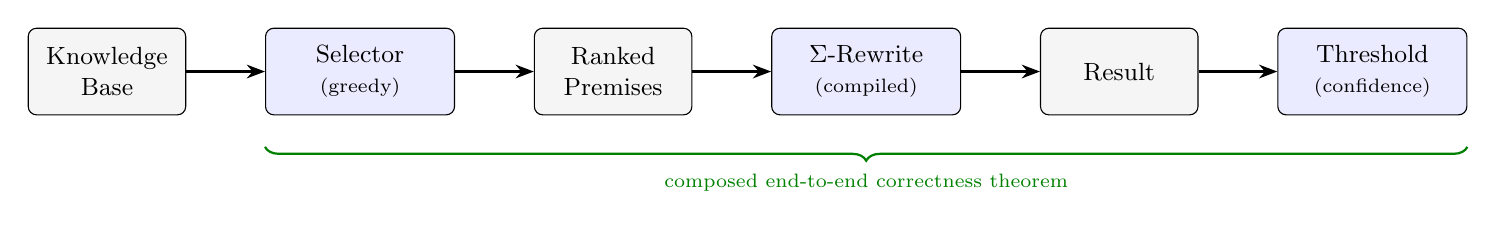
\begin{tikzpicture}[
  >=Stealth,
  every node/.style={font=\small},
  box/.style={draw, rounded corners=3pt, align=center,
              minimum height=11mm},
  stage/.style={box, fill=blue!8, minimum width=24mm},
  data/.style={box, fill=gray!8, minimum width=20mm},
]
\node[data] (kb) {Knowledge\\Base};
\node[stage, right=10mm of kb] (sel) {Selector\\{\scriptsize(greedy)}};
\node[data, right=10mm of sel] (prem) {Ranked\\Premises};
\node[stage, right=10mm of prem] (rew) {$\Sigma$-Rewrite\\{\scriptsize(compiled)}};
\node[data, right=10mm of rew] (res) {Result};
\node[stage, right=10mm of res] (thr) {Threshold\\{\scriptsize(confidence)}};

\draw[->, thick] (kb) -- (sel);
\draw[->, thick] (sel) -- (prem);
\draw[->, thick] (prem) -- (rew);
\draw[->, thick] (rew) -- (res);
\draw[->, thick] (res) -- (thr);

% end-to-end bracket
\draw[decorate, decoration={brace, amplitude=5pt, mirror},
      thick, green!50!black]
  ($(sel.south west) + (0, -4mm)$) --
  node[below=6pt, font=\scriptsize, green!50!black]
    {composed end-to-end correctness theorem}
  ($(thr.south east) + (0, -4mm)$);
\end{tikzpicture}
\caption{The inference-control pipeline.  A selector chooses premises from
the knowledge base; a $\Sigma$-guarded compiled rewrite produces a result;
a threshold accepts or rejects based on confidence.  The composed pipeline
has a single end-to-end correctness theorem.}
\label{fig:inference-control-pipeline}
\end{figure}

\section{Coverage Surrogate Boundaries}

\boundarystart
\begin{theorem}[Coverage/cardinality surrogate no-go (\claimBoundary{})]
Coverage and cardinality together are insufficient for risk-sensitive
selection: there exist premise sets with identical coverage and cardinality
but different false-positive risk.
\end{theorem}
\boundaryend

See \codepath{Mettapedia/Logic/PremiseSelectionCoverageCounterexamples.lean}.

\section{Composed Core Endpoints}

The one-call selector $\to$ rewrite $\to$ threshold composition:
\begin{lstlisting}
ch9_selector_rewrite_threshold_end_to_end_of_interval
\end{lstlisting}

composes the entire pipeline into a single theorem: given a selector that
produces a ranked premise set, a rewrite that applies a PLN rule under
BN side conditions, and a threshold that accepts the result, the composed
pipeline is correct.

See \codepath{Mettapedia/Logic/PLNCanonicalAPI.lean}.


%% ═══════════════════════════════════════════════════════════════════
\part{Natively Typed World Models}
\label{part:ntt}
%% ═══════════════════════════════════════════════════════════════════

\chapter{The World-Model Calculus as a Language Family}
\label{ch:wm-gslt}

\begin{quote}\small
\textbf{Goal:} Package every variant of the WM posterior-state calculus as a
graph-structured language theory (GSLT), derive modal operators via OSLF,
and establish transport theorems between variants.\\
\textbf{Semantic object:} 13-axis vertex family; per-vertex \texttt{LanguageDef};
forward simulation via rule-subset containment; automatic $\Diamond\dashv\Box$
Galois connection.\\
\textbf{Proved (kernel-checked):} All items in this chapter.  0 sorry.\\
\textbf{Assumed:} None beyond the OSLF/TypeSynthesis infrastructure.
\end{quote}

Throughout the preceding chapters, the world-model posterior-state calculus
appears in many guises: additive revision (Chapter~\ref{ch:posterior-state}),
overlap-corrected fusion, scope-based forgetting, support-tracked inverse
forgetting, Kripke provenance tracking, fixpoint closure, conservation
bounds, experiment channels, stochastic decision theory, and generic
carriers.  Each variant shares the same core axioms---evidence additivity,
revision commutativity and associativity, combine commutativity---but adds
its own operations and equational laws.

This chapter shows that this family of variants has a precise algebraic
structure.  Each variant is a \emph{typed language definition}
(\texttt{LanguageDef}) whose rewrite rules encode the variant's equational
theory.  The variants are indexed by a 13-axis vertex
(\texttt{WMFullVertex}), and weaker variants embed into stronger ones via
identity-on-terms forward simulation (the weaker variant's rule set is a
subset of the stronger one's).  The OSLF pipeline then automatically
derives modal operators and a Galois connection per vertex.

\section{Pattern Vocabulary}

The WM calculus is encoded in the OSLF pattern language using three core
sorts---\textbf{State}, \textbf{Query}, \textbf{Evidence}---and
constructors corresponding to the calculus operations:

\begin{center}
\begin{tabular}{lll}
\toprule
\textbf{Constructor} & \textbf{Signature} & \textbf{Operation} \\
\midrule
$\mathsf{Revise}(W_1, W_2)$ & State $\times$ State $\to$ State & parallel composition \\
$\mathsf{Extract}(W, q)$ & State $\times$ Query $\to$ Evidence & observation \\
$\mathsf{Combine}(e_1, e_2)$ & Evidence $\times$ Evidence $\to$ Evidence & additive fusion \\
$\mathsf{Forget}(S, W)$ & Scope $\times$ State $\to$ State & restriction \\
$\mathsf{OverlapMerge}(W_1, W_2)$ & State $\times$ State $\to$ State & overlap-aware merge \\
$\mathsf{FallbackRevision}(W_1, W_2)$ & State $\times$ State $\to$ State & source-gated merge \\
$\mathsf{LeastClosure}(R, W, S)$ & RuleSet $\times$ State $\times$ QuerySet $\to$ QuerySet & fixpoint \\
$\mathsf{SwapAnomaly}(W_1, W_2, q)$ & State$^2$ $\times$ Query $\to$ Evidence & order cost \\
$\mathsf{KripkeEvidence}(W, \varphi)$ & State $\times$ ModalQuery $\to$ Evidence & modal evidence \\
\bottomrule
\end{tabular}
\end{center}

Each extension family introduces additional constructors (30 total across
all families); the table above shows the most important ones.

\section{Core Rewrite Rules}

Five rewrite rules are shared by every variant:

\begin{enumerate}
\item \textbf{Evidence additivity} (\claimCore{}).
  $\mathsf{Extract}(\mathsf{Revise}(W_1, W_2),\, q) \;\leadsto\;
  \mathsf{Combine}(\mathsf{Extract}(W_1, q),\; \mathsf{Extract}(W_2, q))$.
  This is the fundamental WM axiom: evidence extraction distributes over
  revision.

\item \textbf{Revision commutativity} (\claimCore{}).
  $\mathsf{Revise}(W_1, W_2) \;\leadsto\; \mathsf{Revise}(W_2, W_1)$.

\item \textbf{Revision associativity} (\claimCore{}).
  $\mathsf{Revise}(\mathsf{Revise}(W_1, W_2), W_3)
  \;\leadsto\; \mathsf{Revise}(W_1, \mathsf{Revise}(W_2, W_3))$.

\item \textbf{Combine commutativity} (\claimCore{}).
  $\mathsf{Combine}(e_1, e_2) \;\leadsto\; \mathsf{Combine}(e_2, e_1)$.

\item \textbf{Combine identity} (\claimCore{}).
  $\mathsf{Combine}(e, \mathsf{EvidenceZero}) \;\leadsto\; e$.
\end{enumerate}

Each rule is encoded as a \texttt{RewriteRule} structure with a
\texttt{typeContext} (typed metavariables), \texttt{premises} (side
conditions), \texttt{left} and \texttt{right} patterns.  The core rules
have empty premises; in the \emph{raw} (schematic) calculus all extension
rules also have empty premises, while the \emph{guarded} (faithful)
calculus carries real \texttt{Premise.relationQuery} side conditions
(Section~\ref{sec:wm-guarded}).  Sixteen step
lemmas are kernel-checked: 3~core (evidence-add, revision-comm,
revision-assoc) at both extended and full vertices, plus 10~extension-axis
lemmas (overlap, forgetting, exact-inverse, provenance-symmetry,
closure-fixpoint, swap-anomaly, anti-hallucination, experiment,
Kripke, generic carrier).

\section{The 13-Axis Vertex Family}
\label{sec:wm-13axis}

The WM calculus variants are indexed by a 13-axis \texttt{WMFullVertex}:

\begin{center}
\begin{tabular}{rlll}
\toprule
\textbf{\#} & \textbf{Axis} & \textbf{Values} & \textbf{Effect} \\
\midrule
1--4 & Base (logic, tv, interval, typing)
     & $2 \times 2 \times 3 \times 2 = 24$
     & model-level (same rules) \\
5 & Overlap & additive $|$ overlapAware & +1 rule \\
6 & Forgetting & none $|$ scopeBased $|$ supportTracked & +2--3 rules \\
7 & Provenance & none $|$ sourceLabeled & +6 rules \\
8 & Fixpoint & none $|$ closure $|$ policy $|$ cascade & +2--4 rules \\
9 & Cost & none $|$ costTracked & +3 rules \\
10 & Conservation & none $|$ conserving & +2 rules \\
11 & Experiment & none $|$ deterministic $|$ stochastic & +3--7 rules \\
12 & Kripke & none $|$ pointedKripke & +3 rules \\
13 & Carrier & concrete $|$ generic & +2 rules \\
\bottomrule
\end{tabular}
\end{center}

The first four axes are \emph{model-level}: all 24 combinations produce the
same \texttt{LanguageDef} (the same rewrite rules), differing only in
semantic interpretation.  This is proved by \texttt{wmVertexLanguageDef\_eq}
(exhaustive case analysis, kernel-checked).  The remaining nine axes are
\emph{syntactic}: each adds genuinely new rewrite rules.

A 13-axis vertex has $2^{13} = 8{,}192$ possible configurations in the
na\"{\i}ve product, yet the number of distinct rewrite rules grows only
linearly with the number of enabled extensions.  The two extremes pin
down the range:

\begin{theorem}[\texttt{wmFullVertexMinimal\_ruleCount}, kernel-checked]
The minimal vertex (all extensions disabled) has exactly~5 rewrite rules
(the core rules).
\end{theorem}

\begin{theorem}[\texttt{wmFullVertexMaximal\_ruleCount}, kernel-checked]
The maximal vertex (all extensions enabled at strongest level) has exactly~36
rewrite rules.
\end{theorem}

The jump from 5 to 36 is modest---each extension family contributes
between one and six rules---and every intermediate vertex falls
strictly between these bounds.  This linear growth means the OSLF
pipeline (Galois connection, modal operators, step lemmas) scales
gracefully across the entire family.

\section{Extension Families}
\label{sec:wm-extensions}

Each extension family contributes its own rewrite rules:

\paragraph{Overlap (1 rule).}
$\mathsf{Extract}(\mathsf{OverlapMerge}(W_1, W_2), q)
\;\leadsto\; \mathsf{OverlapCorrect}(\mathsf{Extract}(W_1,q),\;
\mathsf{Extract}(W_2,q),\; \mathsf{OverlapFactor}(W_1,W_2,q))$.
This captures the non-additive correction from the overlap layer
(Chapter~\ref{ch:posterior-state}).

\paragraph{Forgetting (2--3 rules).}
Outside-scope invariance:
$\mathsf{Extract}(\mathsf{Forget}(S, W), q)
\;\leadsto\; \mathsf{Extract}(W, q)$ (when $q \notin \mathrm{scope}(S)$).
Idempotence:
$\mathsf{Forget}(S, \mathsf{Forget}(S, W)) \;\leadsto\; \mathsf{Forget}(S, W)$.
Support-tracked mode adds the exact-inverse rule:
$\mathsf{Forget}(S, \mathsf{Revise}(W, \Delta)) \;\leadsto\; W$
(when $\mathrm{support}(\Delta) \subseteq \mathrm{scopeFootprint}(S)$).

\paragraph{Provenance (6 rules).}
Source-compatibility symmetry, fallback decomposition (compatible/incompatible
cases), partial revision, trusted-gate identity
($\mathsf{TrustedGate}(\mathsf{TrustedAll}, W) \leadsto W$), and evidence
additivity under compatible fallback revision.  These encode the
\texttt{KripkeWeightedOverlap} layer's operations.

\paragraph{Fixpoint (2--4 rules).}
Closure fixpoint:
$\mathsf{ImmediateStep}(R, W, S, \mathsf{LeastClosure}(R, W, S))
\;\leadsto\; \mathsf{LeastClosure}(R, W, S)$.
Iteration unfolding.  Policy-driven mode adds the trusted-all simplification.
Cascade mode adds the cardinality-bounded stabilization:
$\mathsf{ImmediateIter}(R, W, S, \mathsf{Card}(Q))
\;\leadsto\; \mathsf{LeastClosure}(R, W, S)$.

\paragraph{Cost (3 rules).}
Swap anomaly symmetry, swap anomaly zero (when observation counts are equal),
and schedule error symmetry.

\paragraph{Conservation (2 rules).}
Anti-hallucination:
$\mathsf{Extract}(\Delta, q) \;\leadsto\; \mathsf{EvidenceZero}$
(when $q$ is outside scope and exact-inverse holds).
Noether conservation:
$\mathsf{Extract}(\mathsf{Revise}(W, \Delta), q) \;\leadsto\;
\mathsf{Extract}(W, q)$ (outside scope).

\paragraph{Experiment channels (3--7 rules).}
Experiment evidence additivity, Blackwell factorization pullback, channel
composition identity.  Stochastic mode adds stochastic evidence additivity,
channel composition associativity, Blackwell utility transport, and Kleisli
identity.

\paragraph{Kripke (3 rules).}
Kripke evidence additivity, singleton satisfaction
($\mathsf{KripkeEvidence}(\mathsf{Singleton}(pk), \varphi) \leadsto
\mathsf{EvidenceOne}$ when $pk \models \varphi$), and singleton refutation.

\paragraph{Generic carriers (2 rules).}
Generic evidence additivity (the core axiom in abstract carrier form)
and query-equivalence transport.

\section{Forward Simulation and Transport}

\begin{theorem}[\texttt{wmFullVertexLanguageDef\_base\_eq}, kernel-checked]
For any two full vertices $v, w$ with identical extension axes (axes~5--13),
$\mathsf{wmFullVertexLanguageDef}(v) = \mathsf{wmFullVertexLanguageDef}(w)$.
The base~4 axes do not affect the rewrite rules.
\end{theorem}

Forward simulation between vertices with different extension axes follows
from rule-subset containment: if vertex~$v$ has fewer rules than vertex~$w$,
then every reduction at~$v$ is also a reduction at~$w$ (both use the same
pattern vocabulary with $\mathsf{mapTerm} = \mathrm{id}$).

For the 4-axis base case, all vertices produce literally the same
\texttt{LanguageDef}, so reductions transfer freely:

\begin{theorem}[\texttt{wmCalc\_transport}, kernel-checked]
For any $v, w : \mathsf{WMVertex}$ and any reduction chain
$p \to^* q$ at vertex~$v$, the same chain is a valid reduction at
vertex~$w$.
\end{theorem}

\section{OSLF-Derived Modal Operators}
\label{sec:wm-oslf}

Passing any vertex's \texttt{LanguageDef} through the OSLF pipeline
(\texttt{langOSLF}) automatically derives:

\begin{itemize}
\item \textbf{Diamond ($\Diamond\varphi$)}: holds at pattern~$p$ iff
  $\exists q.\; p \leadsto q \wedge \varphi(q)$.
  ``This WM expression can be rewritten to one satisfying~$\varphi$.''

\item \textbf{Box ($\Box\varphi$)}: holds at pattern~$p$ iff
  $\forall q.\; q \leadsto p \to \varphi(q)$.
  ``All expressions that reduce \emph{to}~$p$ satisfy~$\varphi$.''

\item \textbf{Galois connection} $\Diamond \dashv \Box$
  (\texttt{langGalois}, automatic):
  $(\forall p.\; p \in \Diamond\varphi \Rightarrow p \in \psi)
  \;\Leftrightarrow\;
  (\forall p.\; p \in \varphi \Rightarrow p \in \Box\psi)$.
\end{itemize}

These operators have concrete evidence-theoretic meaning:

\begin{description}
\item[Evidence reachability ($\Diamond$).]
  $\Diamond(\mathsf{isCombined})$ holds at any
  $\mathsf{Extract}(\mathsf{Revise}(W_1, W_2), q)$ because the
  evidence-add rule rewrites it to a $\mathsf{Combine}$ term.

\item[Evidence safety ($\Box$).]
  $\Box(\mathsf{isPositive})$ at pattern~$p$ means every expression that
  reduces to~$p$ was already positive---a backward safety guarantee.

\item[Vertex dependence.]
  At the minimal vertex (5~rules), $\Diamond$ is small (few rewrites
  reachable).  At the maximal vertex (36~rules), $\Diamond$ is much
  larger: overlap correction, forgetting, fixpoint closure, Blackwell
  factorization all become reachable.  The Galois connection tightens:
  more $\Diamond$ means weaker~$\Box$.

\item[Conservation as $\Box$-safety.]
  With conservation rules enabled, $\Box(\text{outsideScope} \Rightarrow
  \text{preserved})$ holds at any $\mathsf{Revise}(W, \Delta)$: backward
  safety captures the Noether-style conservation guarantee.
\end{description}

\section{Formalization Inventory}

All results in this chapter are kernel-checked in Lean~4.28 (0~sorry):

\begin{center}
\begin{tabular}{lll}
\toprule
\textbf{File} & \textbf{Contents} & \textbf{Status} \\
\midrule
\texttt{WMCalculusLanguageDef.lean}
  & 37 raw + 17 guarded rewrite rules, 7 axis types,
    \texttt{WMFullVertex}, 16 step lemmas, guarded LanguageDefs
  & proved \\
\texttt{WMCalculusGSLTVertex.lean}
  & fiber, transport, rule counts, OSLF per vertex
  & proved \\
\texttt{PLNWMHypercubeBasis.lean}
  & 4-axis \texttt{WMVertex}, \texttt{CubePath}, transport
  & proved \\
\texttt{WMProbabilityEmbedding.lean}
  & 13-axis probability embedding, monotonicity
  & proved \\
\texttt{WMCalculusOSLFBridge.lean}
  & semantic bridge: $\Diamond$ theorems, Galois corollaries,
    \texttt{WMTermEncodes}, barbs, chaining,
    guarded Galois connections
  & proved \\
\texttt{WMCalculusContextClosure.lean}
  & 15 congruence rules, context closure LanguageDefs,
    raw $\subseteq$ cong-extended, Galois for extended calculi
  & proved \\
\texttt{WMCalculusEncoding.lean}
  & \texttt{encodeWM}, roundtrip, injectivity,
    \texttt{WMStep} soundness + completeness on image
  & proved \\
\texttt{WMCalculusNeighborhoodBridge.lean}
  & neighborhood fiber: evidence-add correspondence,
    $\Diamond$ decomposition, singleton adequacy, Galois
  & proved \\
\texttt{WMCalculusFOLBridge.lean}
  & FOL fiber: Tarskian evidence correspondence,
    validity, model-theoretic consequence bridge
  & proved \\
\bottomrule
\end{tabular}
\end{center}

\section{Guarded Calculus}
\label{sec:wm-guarded}

The extension rules (axes~5--13) carry informal side conditions documented
in docstrings---for example, the forgetting rule
$\mathsf{Extract}(\mathsf{Forget}(S,W), q) \leadsto \mathsf{Extract}(W, q)$
requires ``$q \notin \mathrm{scope}(S)$'' but this condition was not checked
by the rewrite engine.

The \emph{guarded calculus} makes these side conditions explicit as
\texttt{Premise.relationQuery} entries.  For each extension rule with an
informal side condition, a parallel guarded variant is defined with the
appropriate \texttt{premises} field.  The 5~core rules have no premises
and are shared between both families.

\begin{center}
\begin{tabular}{ll}
\toprule
\textbf{Calculus} & \textbf{Description} \\
\midrule
Raw (\texttt{wmExtVertexLanguageDef}) & schematic: all rules fire unconditionally \\
Guarded (\texttt{wmExtVertexLanguageDefGuarded}) & faithful: extension rules carry real premises \\
\bottomrule
\end{tabular}
\end{center}

The raw calculus is an overapproximation of the guarded one---every guarded
reduction is also a raw reduction (dropping premises only enables more
reductions).  The OSLF pipeline produces a Galois connection
$\Diamond \dashv \Box$ for both:

\begin{theorem}[\texttt{wmGuardedCalc\_galois}, kernel-checked]
For any \texttt{RelationEnv} and extended vertex~$v$:
$\Diamond_{\mathit{guarded}} \dashv \Box_{\mathit{guarded}}$.
\end{theorem}

\noindent
See \codepath{Mettapedia/OSLF/Framework/WMCalculusLanguageDef.lean} (17~guarded
rules) and \codepath{Mettapedia/OSLF/Framework/WMCalculusOSLFBridge.lean}.

\section{Context Closure via Congruence Rules}
\label{sec:wm-context-closure}

The core WM patterns use \texttt{.apply} constructors (not
\texttt{.collection}), so the engine's built-in \texttt{congElem}
constructor---which only descends into \texttt{.collection} nodes---never
fires on WM terms.  Without explicit congruence rules, reductions cannot
propagate into subterms.

The congruence extension adds 15~explicit rewrite rules, one per argument
position of each WM constructor:

\begin{center}
\begin{tabular}{ll}
\toprule
\textbf{Constructor} & \textbf{Congruence rules} \\
\midrule
$\mathsf{Revise}(W_1, W_2)$ & left, right \\
$\mathsf{Extract}(W, q)$ & left, right \\
$\mathsf{Combine}(e_1, e_2)$ & left, right \\
$\mathsf{Forget}(S, W)$ & right \\
$\mathsf{OverlapMerge}(W_1, W_2)$ & left, right \\
Extension constructors & 6 more \\
\bottomrule
\end{tabular}
\end{center}

Each congruence rule uses \texttt{Premise.congruence src tgt}, which
checks that \texttt{src} reduces to \texttt{tgt} via the no-premises engine
path.  In the raw calculus, congruence descends through all reductions.
In the guarded calculus, only unconditional rules propagate through
congruence; side-conditioned extension rules do not fire inside subterms
unless independently satisfied.

\begin{theorem}[\texttt{congReduces\_of\_rawReduces\_ext}, kernel-checked]
Every raw reduction is also a congruence-extended reduction (rule-set
inclusion).
\end{theorem}

\noindent
The context-closure module also completes the \textbf{2\texttimes 2 calculus
square}: \{Raw, Guarded\} \texttimes\ \{Plain, +Cong\}.
The guarded+cong definitions (\texttt{wmExtVertexLanguageDefGuardedWithCong}
and the full-vertex variant) add congruence rules on top of the guarded
calculus.  All four horizontal and vertical inclusion arrows are
kernel-checked, and Galois connections hold at every corner.

\begin{theorem}[\texttt{chain\_evidence\_add\_fully\_nested}, kernel-checked]
In the cong-extended calculus, the term
$\mathsf{Extract}(\mathsf{Revise}(\mathsf{Revise}(W_1, W_2), W_3),\; q)$
reduces in \emph{two} steps to
$\mathsf{Combine}(\mathsf{Combine}(\mathsf{Extract}(W_1,q),\;
\mathsf{Extract}(W_2,q)),\; \mathsf{Extract}(W_3,q))$.
Step~1 applies evidence-add to the outer $\mathsf{Revise}$;
Step~2 uses \texttt{ruleCombineCongLeft} to apply evidence-add
\emph{inside} the left $\mathsf{Combine}$ argument.
The congruence premise is satisfied because the inner evidence-add
has empty premises and is therefore witnessed by
\texttt{rewriteWithContextNoPremises}.
Full-vertex and guarded+cong variants are also kernel-checked.
\end{theorem}

\noindent
See \codepath{Mettapedia/OSLF/Framework/WMCalculusContextClosure.lean}
(463~lines, 0~sorry) and
\codepath{Mettapedia/OSLF/Framework/WMCalculusOSLFBridge.lean}
(784~lines, 0~sorry).

\section{Encoding Faithfulness on the Image}
\label{sec:wm-encoding}

The abstract syntax is given by an \emph{intrinsically sorted} type family
$\mathsf{WMTerm} : \mathsf{WMSort} \to \mathsf{Type}$, where
$\mathsf{WMSort} = \{\mathsf{state},\; \mathsf{query},\;
\mathsf{evidence}\}$.
States and queries both encode to free variables
($\mathsf{state}\;x,\;\mathsf{query}\;x \;\mapsto\; \mathtt{.fvar}\;x$),
but they carry \emph{different sort indices}, so injectivity holds
within each sort:

\begin{theorem}[\texttt{encodeWM\_injective}, kernel-checked]
\label{thm:encode-injective}
For any sort~$s$ and terms $t_1, t_2 : \mathsf{WMTerm}\;s$,\;
$\mathtt{encodeWM}\;t_1 = \mathtt{encodeWM}\;t_2
\;\Rightarrow\; t_1 = t_2$.
\end{theorem}

\noindent
The sort index also makes subject reduction \emph{definitional}: every
constructor of $\mathsf{WMStep} : \mathsf{WMTerm}\;s \to
\mathsf{WMTerm}\;s \to \mathsf{Prop}$ preserves the sort by
construction.  The five constructors (evidence-add, revision-comm,
revision-assoc, combine-comm, combine-zero) correspond one-to-one to
the 5~core rewrite rules.

\begin{theorem}[Biconditional, \texttt{wmStep\_iff}, kernel-checked]
\label{thm:wmstep-iff}
$\mathsf{WMStep}\;t_1\;t_2 \;\Leftrightarrow\;
\mathtt{langReduces}\;\mathtt{wmCoreLanguageDef}\;
(\mathtt{encodeWM}\;t_1)\;(\mathtt{encodeWM}\;t_2)$.
\end{theorem}

\noindent
The forward direction (\texttt{wmStep\_sound}) constructs the
$\mathtt{DeclReducesWithPremises}$ witness; the backward direction
(\texttt{wmStep\_complete}) eliminates the $\mathtt{congElem}$ case
(WM patterns are $\mathtt{.apply}$, not $\mathtt{.collection}$) and
inverts $\mathtt{matchPattern}$ on each of the 5~core rules.

\subsection{Star Adequacy}
\label{sec:wm-star-adequacy}

The biconditional lifts to multi-step reductions.
Define $\mathsf{WMStepStar} := \mathtt{ReflTransGen}\;\mathsf{WMStep}$
(Lean's reflexive-transitive closure).

\begin{theorem}[Star adequacy, \texttt{wmStepStar\_adequate}, kernel-checked]
\label{thm:star-adequate}
$\mathsf{WMStepStar}\;t_1\;t_2 \;\Leftrightarrow\;
\mathtt{LangReducesStar}\;\mathtt{wmCoreLanguageDef}\;
(\mathtt{encodeWM}\;t_1)\;(\mathtt{encodeWM}\;t_2)$.
\end{theorem}

\noindent
The forward direction (\texttt{wmStepStar\_sound}) is a straightforward
induction on $\mathtt{ReflTransGen}$ using single-step soundness.  The
backward direction (\texttt{wmStepStar\_complete}) requires a
\emph{generalization trick}: since $\mathtt{LangReducesStar}$ carries
$\mathtt{encodeWM}\;t_1$ as a non-variable index, we first generalize
it to a fresh variable~$p$ before inducting, then recover the
$\mathsf{WMTerm}$-level witness at each step via single-step
completeness and injectivity (Theorem~\ref{thm:encode-injective}).

\subsection{Modal Lifting and a Backward Asymmetry}
\label{sec:wm-backward-asymmetry}

The biconditional (Theorem~\ref{thm:wmstep-iff}) yields a sound
$\Box$-lifting theorem: any $\mathtt{langBox}$ property at
$\mathtt{encodeWM}\;t$ can be pulled back to all $\mathsf{WMStep}$
predecessors.

\begin{theorem}[\texttt{wmBox\_sound}, kernel-checked]
If $\mathtt{langBox}\;\mathtt{wmCoreLanguageDef}\;\varphi\;(\mathtt{encodeWM}\;t)$,
then $\varphi(\mathtt{encodeWM}\;t')$ for every
$t' : \mathsf{WMTerm}\;s$ with $\mathsf{WMStep}\;t'\;t$.
\end{theorem}

\noindent
However, the converse---\emph{backward completeness}---is \textbf{false}
for intrinsically sorted terms.
The obstacle is that the Pattern-level reduction system admits
predecessors \emph{outside the image} of $\mathtt{encodeWM}$.
For example, $\mathtt{ruleCombineZero}$ (whose right-hand side is
$\mathtt{.fvar}\;\texttt{"e"}$) produces the Pattern-level predecessor
$\mathtt{pCombine}\;(\mathtt{.fvar}\;\texttt{"x"})\;\mathtt{pEvidenceZero}$
at $\mathtt{.fvar}\;\texttt{"x"}$---but $\mathtt{.fvar}\;\texttt{"x"}$
is the encoding of a \emph{leaf} term ($\mathsf{state}$ or
$\mathsf{query}$), which has no $\mathsf{WMStep}$ predecessor with a
$\mathsf{combine}$ head.
The ``junk predecessors'' are artifacts of
the universal-quantifier pattern variables in the rewrite rules and
cannot be eliminated without restricting the OSLF reduction relation
itself.

This asymmetry is harmless: the $\Diamond$~direction (forward
completeness) suffices for all evidence-theoretic applications, and
$\Box$~soundness already allows pulling modal properties back to the
abstract level.

\noindent
See \codepath{Mettapedia/OSLF/Framework/WMCalculusEncoding.lean}
(497~lines, 0~sorry).

\section{Semantic Bridge: From $\Diamond/\Box$ to Evidence Theory}
\label{sec:wm-gslt-bridge}

The syntactic layer (rewrite rules, step lemmas, OSLF-derived $\Diamond/\Box$)
is now connected to the WorldModel evidence-theoretic operations via a
\emph{semantic bridge} (\texttt{WMCalculusOSLFBridge.lean}, 0~sorry,
kernel-checked).  The bridge has three layers.

\subsection{Layer 1: Diamond Theorems via Step Lemmas}

Pattern predicates capture evidence-theoretic properties syntactically:

\begin{center}
\begin{tabular}{ll}
\toprule
\textbf{Predicate} & \textbf{Meaning} \\
\midrule
$\mathsf{isCombined}(p)$ & $p = \mathsf{Combine}(e_1, e_2)$ \\
$\mathsf{isDecomposable}(p)$ & $p = \mathsf{Extract}(\mathsf{Revise}(W_1, W_2), q)$ \\
$\mathsf{isRevision}(p)$ & $p = \mathsf{Revise}(W_1, W_2)$ \\
$\mathsf{isFixpoint}(p)$ & $p = \mathsf{LeastClosure}(R, W, S)$ \\
$\mathsf{isOverlapCorrected}(p)$ & $p = \mathsf{OverlapCorrect}(e_1, e_2, f)$ \\
$\mathsf{isZeroEvidence}(p)$ & $p = \mathsf{EvidenceZero}$ \\
\bottomrule
\end{tabular}
\end{center}

Each $\Diamond$~theorem composes a step lemma with the predicate.  For
example, the core evidence decomposition:

\begin{theorem}[\texttt{diamond\_isCombined\_at\_decomposable}, kernel-checked]
For any WM vertex~$v$ and patterns $W_1, W_2, q$:
\[
  \Diamond(\mathsf{isCombined})\;\text{holds at}\;
  \mathsf{Extract}(\mathsf{Revise}(W_1, W_2),\; q).
\]
\end{theorem}

\noindent
The proof is a single composition: the evidence-add step lemma provides the
witness~$\mathsf{Combine}(\mathsf{Extract}(W_1,q), \mathsf{Extract}(W_2,q))$,
which satisfies $\mathsf{isCombined}$ by construction.

Similar $\Diamond$~theorems hold for all 9~extension axes:
\begin{itemize}
\item \texttt{full\_diamond\_overlapCorrected}: overlap-aware $\Rightarrow$
  $\Diamond(\mathsf{isOverlapCorrected})$ at overlap-merge extracts.
\item \texttt{full\_diamond\_closureFixpoint}: fixpoint-enabled $\Rightarrow$
  $\Diamond(\mathsf{isFixpoint})$ at immediate-step terms.
\item \texttt{full\_diamond\_antiHallucination}: conserving vertex $\Rightarrow$
  $\Diamond(\mathsf{isZeroEvidence})$ at out-of-scope extracts (anti-hallucination).
\item \texttt{full\_diamond\_experimentDecomposable},
  \texttt{full\_diamond\_kripkeDecomposable},
  \texttt{full\_diamond\_genericDecomposable}: extension-specific evidence additivity.
\end{itemize}

\subsection{Layer 2: Relational Encoding and Soundness}

A relational encoding connects abstract WorldModel terms to OSLF patterns:

\begin{center}
\begin{tabular}{l}
\textbf{inductive} $\mathsf{WMTermEncodes} : \mathsf{Pattern} \to \mathsf{WMTerm} \to \mathsf{Prop}$ \\
\quad $\mid$ \texttt{state}$(n)$ : $\mathsf{WMTermEncodes}\;(\mathsf{fvar}\;n)\;(\mathsf{state}\;n)$ \\
\quad $\mid$ \texttt{revise} : $\mathsf{WMTermEncodes}\;p_1\;t_1 \to \mathsf{WMTermEncodes}\;p_2\;t_2$ \\
\quad\quad\quad $\to \mathsf{WMTermEncodes}\;(\mathsf{pRevise}\;p_1\;p_2)\;(\mathsf{revise}\;t_1\;t_2)$ \\
\quad $\mid$ \texttt{extract}, \texttt{combine}, \texttt{query}, \texttt{zero} \ldots
\end{tabular}
\end{center}

\begin{theorem}[\texttt{wm\_evidence\_add\_sound}, kernel-checked]
If $p_{W_1}$ encodes $t_{W_1}$, $p_{W_2}$ encodes $t_{W_2}$, and $p_q$
encodes $t_q$, then there exists a pattern~$q'$ such that
$\mathsf{langReduces}(\mathsf{wmExtVertexLanguageDef}(v),\;
\mathsf{pExtract}(\mathsf{pRevise}(p_{W_1}, p_{W_2}),\; p_q),\; q')$
and $q'$ encodes $\mathsf{combine}(\mathsf{extract}(t_{W_1}, t_q),\;
\mathsf{extract}(t_{W_2}, t_q))$.
\end{theorem}

\noindent
Analogous soundness theorems hold for revision commutativity and
associativity.  The encoding composes with $\Diamond$~theorems:

\begin{theorem}[\texttt{diamond\_isCombined\_of\_encoded}, kernel-checked]
If a pattern~$p$ encodes a term $\mathsf{extract}(\mathsf{revise}(t_1,t_2), t_q)$,
then $\Diamond(\mathsf{isCombined})$ holds at~$p$.
\end{theorem}

\subsection{Layer 3: Galois Corollaries}

The Galois connection $\Diamond \dashv \Box$ instantiates to concrete
evidence-theoretic dualities:

\begin{theorem}[\texttt{wmCalc\_decomposability\_safety}, kernel-checked]
$(\forall p.\; \Diamond(\mathsf{isCombined})(p) \Rightarrow \psi(p))
\;\Leftrightarrow\;
(\forall p.\; \mathsf{isCombined}(p) \Rightarrow \Box(\psi)(p))$.
\end{theorem}

\noindent
Reading: ``every combined state reachable by forward rewriting satisfies~$\psi$''
is equivalent to ``every combined state has all its backward predecessors
satisfying~$\psi$.''  Similar corollaries hold for overlap, fixpoint, and
conservation predicates.

\subsection{Diamond Chaining}

Multi-step rewrite chains compose via $\mathsf{LangReducesStar}$:

\begin{theorem}[\texttt{chain\_evidence\_add\_nested}, kernel-checked]
Given patterns $W_1, W_2, W_3, q$, the term
$\mathsf{Extract}(\mathsf{Revise}(\mathsf{Revise}(W_1, W_2), W_3),\; q)$
reduces in one step to
$\mathsf{Combine}(\mathsf{Extract}(\mathsf{Revise}(W_1,W_2),\,q),\;
\mathsf{Extract}(W_3,q))$.
The inner $\mathsf{Revise}(W_1,W_2)$ is \emph{not} further decomposed
at this stage.
\end{theorem}

\noindent
Full decomposition to
$\mathsf{Combine}(\mathsf{Combine}(\mathsf{Extract}(W_1,q),\;
\mathsf{Extract}(W_2,q)),\; \mathsf{Extract}(W_3,q))$
requires applying the evidence-add rule \emph{under a context}---specifically
inside the left argument of $\mathsf{Combine}$.  The theorem
\texttt{chain\_evidence\_add\_fully\_nested} (Section~\ref{sec:wm-context-closure})
achieves this via the congruence infrastructure of the context-closure calculus.

The chaining infrastructure also gives \texttt{chain\_assoc\_then\_comm}
(reassociate then commute) and full-vertex variants.

\subsection{Evidence Barbs (Process-Algebraic Observables)}

Following Milner's barbed bisimulation, we define a WM-specific observable:

\begin{definition}[\texttt{wmHasEvidenceBarb}]
A state~$W$ \emph{exhibits an evidence barb for query~$q$} when
$\mathsf{Extract}(W, q)$ reduces to a non-zero evidence term:
$\exists e.\; \mathsf{Extract}(W,q) \leadsto e \;\wedge\; e \neq \mathsf{EvidenceZero}$.
\end{definition}

\begin{theorem}[\texttt{wmRevisedState\_evidenceBarb}, kernel-checked]
$\mathsf{Revise}(W_1, W_2)$ exhibits an evidence barb for~$q$ whenever
$\mathsf{Combine}(\mathsf{Extract}(W_1,q), \mathsf{Extract}(W_2,q))$ is
non-zero---i.e., the evidence-add rule provides the witness.
\end{theorem}

\subsection{Neighborhood Semantics Fiber}

The abstract LanguageDef reductions correspond exactly to concrete
model-theoretic facts when instantiated at the neighborhood WorldModel
instance (\texttt{PLNWorldModelNeighborhood.lean}).

A \emph{NeighborhoodValuation} maps WMTerm string names to concrete objects:
\texttt{stateVal : String $\to$ Multiset PointedNeighborhood} and
\texttt{queryVal : String $\to$ ModalQuery}.

\begin{theorem}[\texttt{neighborhood\_evidence\_add\_correspondence}, kernel-checked]
The LanguageDef reduction
$\mathsf{Extract}(\mathsf{Revise}(W_1, W_2), q) \leadsto
\mathsf{Combine}(\mathsf{Extract}(W_1, q), \mathsf{Extract}(W_2, q))$
and the mathematical identity
$\mathsf{neighborhoodEvidence}(W_1 + W_2, \varphi) =
\mathsf{neighborhoodEvidence}(W_1, \varphi) +
\mathsf{neighborhoodEvidence}(W_2, \varphi)$
are corresponding facts (both hold simultaneously).
\end{theorem}

\noindent
Further theorems lift through the valuation: $\Diamond$~decomposition
of evidence into per-source satisfaction counts,
singleton adequacy ($\mathsf{pn.satisfies}(\varphi) \Leftrightarrow
\mathsf{queryStrength}(\{pn\}, \varphi) = 1$),
evidence barbs for revised states, and the Galois corollary
$\Diamond \dashv \Box$ with neighborhood-semantic reading.

See \codepath{Mettapedia/OSLF/Framework/WMCalculusNeighborhoodBridge.lean}
(230~lines, 0~sorry).

\subsection{First-Order Logic Fiber}

The parallel FOL fiber connects the LanguageDef to the Tarskian
WorldModel instance (\texttt{PLNWorldModelFOL.lean}).

A \emph{FOLValuation~$L$} maps state names to
$\mathsf{Multiset}(\mathsf{PointedFOL}\;L)$ and query names to
$\mathsf{FOLQuery}\;L$ (first-order sentences over language~$L$).

\begin{theorem}[\texttt{fol\_evidence\_add\_correspondence}, kernel-checked]
The same evidence-add correspondence holds for Tarskian satisfaction
counting: the syntactic reduction and
$\mathsf{folEvidence}(W_1 + W_2, \varphi) =
\mathsf{folEvidence}(W_1, \varphi) + \mathsf{folEvidence}(W_2, \varphi)$
are the same fact in two formalisms.
\end{theorem}

\noindent
The FOL fiber additionally proves:

\begin{itemize}
\item \textbf{Validity as maximal strength}: if all structures satisfy the query
  and the state is non-empty, query strength equals~1.
\item \textbf{Model-theoretic consequence bridge}: FOL semantic consequence
  ($\forall S.\; S \models \varphi \Rightarrow S \models \psi$) corresponds
  exactly to WM strength ordering
  ($\mathsf{queryStrength}(W, \varphi) \le \mathsf{queryStrength}(W, \psi)$),
  and the converse holds at singletons (fully faithful).
\end{itemize}

\noindent
See \codepath{Mettapedia/OSLF/Framework/WMCalculusFOLBridge.lean}
(295~lines, 0~sorry).

\subsection{Remaining Future Work}

One direction remains open:

\begin{itemize}
\item \textbf{Box-closure theorems ($\Box$ direction)}: proving $\Box\varphi$
  requires showing \emph{all} predecessors satisfy~$\varphi$, which needs
  exhaustive case analysis over the rule set.  A generic
  \texttt{box\_by\_rule\_exhaustion} tactic would make this feasible.
\end{itemize}

\noindent
Two previously open items are now resolved:
\begin{itemize}
\item \textbf{Encoding completeness} (\emph{done}): \texttt{WMCalculusEncoding.lean}
  proves both soundness and completeness on the image of \texttt{encodeWM},
  giving a true biconditional between \texttt{WMStep} and \texttt{langReduces}
  (via intrinsically sorted terms), plus multi-step star adequacy
  (Section~\ref{sec:wm-encoding}).
\item \textbf{Context closure} (\emph{done}): \texttt{WMCalculusContextClosure.lean}
  adds 15~congruence rules enabling reductions inside WM subterms
  (Section~\ref{sec:wm-context-closure}).
\end{itemize}

See \codepath{Mettapedia/OSLF/Framework/WMCalculusOSLFBridge.lean},
\codepath{Mettapedia/OSLF/Framework/WMCalculusLanguageDef.lean},
\codepath{Mettapedia/OSLF/Framework/WMCalculusEncoding.lean},
\codepath{Mettapedia/OSLF/Framework/WMCalculusContextClosure.lean}, and
\codepath{Mettapedia/OSLF/Framework/WMCalculusGSLTVertex.lean}.


%% ═══════════════════════════════════════════════════════════════════
\part{Artifact, Scope, and Relation to PLN}
\label{part:artifact}
%% ═══════════════════════════════════════════════════════════════════

\chapter{What \xiPLN{} Proves}
\label{ch:what-proved}

This chapter provides a compact, family-level summary of the
formalization---what is actually proved, in the Lean kernel, as opposed to
merely discussed or conjectured.

\section{The Kernel}

The foundation is a world-model interface with evidence compositionality:
revision of two world-model states and subsequent query extraction must
agree with extracting from each state separately and then combining the
evidence.  This interface is instantiated concretely by a Dirichlet
reference instance with query extraction over finite world-sets, and the
resulting system admits a sequent-style calculus in which query-revision
is an admissible rule.  The local-completeness no-go theorem
(Chapter~\ref{ch:no-go}) then demonstrates that no link-local evidence
representation can recover full joint evidence---a sharp boundary on the
ambitions of any PLN-like system.

\section{Views and Evidence}

Evidence carries algebraic structure: the formalization proves that
evidence forms both a quantale (with a tensor product modelling revision)
and a Heyting algebra (with implication modelling conditional evidence).
The truth-value views---simple truth values, indefinite truth values, and
distributional views---are all formalized as typed projections from
evidence, with an explicit separation of Walley predictive intervals from
Bayesian credible intervals.  Two convergence bridges ground the
asymptotic story: de~Finetti's exchangeability theorem justifies count
sufficiency, and a Solomonoff convergence bridge shows that evidence
counts approximate the universal posterior.  A Knuth--Skilling
valuation-algebra bridge connects the evidence algebra to information-
theoretic valuations.

\section{Compiled Inference}

The extensional inference rules of classical PLN---deduction, induction,
abduction---are proved exact for the chain, fork, and collider BN motifs
under explicit screening-off and positivity conditions.  D-separation
discharge is packaged as a typeclass, so that a user need only declare the
BN structure and the side conditions are checked automatically.  The Xi
rule registry collects these compiled rewrites with their typed BN
constructor lifts, and a one-call pipeline composes selector, rewrite, and
threshold into a single certified step.  Threshold transport with
explicit boundaries ensures that confidence gates compose correctly
across inference chains.

\section{Extensions}

Higher-order reduction is formalized with corrected side conditions,
together with certified higher-order chaining from estimated variables:
information-set typing, law-of-total-variance reveal, Bayesian regime
update, calibration contracts, certified continue/reveal/fallback/abstain
rules, and stronger root-sum-of-squares bounds under explicit
assumptions.  Finite-model quantifier and fuzzy quantifier semantics
are proved in the weakness-based formulation.  Intensional inheritance
is grounded through typed WM channels (ASSOC and PAT), and
temporal/causal inference is formalized as another WM instance rather than
a separate ontology.

\section{Large-Scale Inference and Control}

Multideduction is formalized via a residual decomposition that makes the
inclusion-exclusion error explicit, together with an identifiability no-go
showing that the residual cannot in general be recovered from local
information.  The trail-free deterministic update protocol admits a
counterexample (a 2-cycle that never stabilizes), but damped convergence
under eventual fresh evidence is proved.  Pooling uniqueness under
external Bayesianity pins down the fusion rule, and BRGI optimization
with feasible-set characterization provides the scheduling foundation.

Premise-selection coverage is proved submodular, yielding the classical
greedy $(1 - 1/e)$ approximation guarantee, while a coverage surrogate
no-go shows that no purely local surrogate can faithfully approximate
global coverage.  A family of five certified-chaining no-go theorems
(Section~\ref{sec:certified-chaining-nogo})---coverage collapse,
Lipschitz sensitivity amplification, variance accumulation,
topology--CPT gap, and regime underdetermination---characterizes the
fundamental limitations of composing per-step certificates.  The current
canonical surface also includes strengthened parametric forms and their
higher-order bridges: graph-parametric topology/CPT impossibility,
chain-with-resets variance accumulation, topology-only
non-certification, and unrevealed-chain variance-budget consumption.

\section{WM-OSLF Bridge}

The world-model calculus is encoded as a 13-axis \texttt{LanguageDef}
family with 36 rewrite rules (5~core + 31~extension), indexed by vertex.
Kernel-checked rule counts confirm the range: 5 at the minimal vertex,
36 at the maximal.  Sixteen step lemmas cover the three core operations
(evidence-add, revision-comm, revision-assoc) across both ext and full
vertices, plus ten extension-axis lemmas for overlap, forgetting,
provenance, fixpoint, cost, conservation, experiment, Kripke, and generic
carrier.

Twelve diamond theorems establish reachability properties:
$\Diamond(\mathsf{isCombined})$, $\Diamond(\mathsf{isCommuted})$,
$\Diamond(\mathsf{isReassociated})$,
$\Diamond(\mathsf{isOverlapCorrected})$,
$\Diamond(\mathsf{isFixpoint})$, $\Diamond(\mathsf{isZeroEvidence})$
(anti-hallucination), and three evidence-decomposition variants for
experiment, Kripke, and generic contexts.  A relational encoding
($\mathsf{WMTermEncodes}$) with soundness theorems and a computable
$\mathsf{encodeWM}$ with one-step completeness on the image provide the
encoding-faithfulness layer.  Four Galois corollaries instantiate the
$\Diamond\dashv\Box$ adjunction for decomposability, overlap, fixpoint,
and conservation safety.  Three diamond-chaining theorems compose
multi-step reductions via $\mathsf{LangReducesStar}$.

The bridge includes two semantic fibers.  A neighborhood fiber connects
LanguageDef reductions to neighborhood-semantic evidence additivity,
$\Diamond$~decomposition, singleton adequacy, and a Galois corollary.
A parallel FOL fiber bridges to Tarskian satisfaction counting, proving
validity-as-maximal-strength and model-theoretic consequence
$\Leftrightarrow$ WM strength ordering (fully faithful at singletons).
Evidence barbs provide a process-algebraic observable for non-zero
evidence extraction.

\section{Cross-Cutting}

The formalization establishes bridges to several neighboring frameworks.
The PLN--NARS bridge proves confidence transforms, rule correspondences,
revision coherence, and an informativeness adjunction between the two
systems.  MeTTa parity theorems verify executable formula parity between
Lean theorems and MeTTa truth functions.  The naive Bayes bridge
(Theorem~\ref{thm:nb-bridge}) and k-NN bridge
(Theorem~\ref{thm:knn-bridge}) show that standard ML classifiers are
special cases of the world-model query machinery.

The ProbLog bridge proves that the world-model infrastructure subsumes
ProbLog distribution semantics exactly:
\[
  \strength(\mathrm{probLogToJointEvidence}(p), q) = \mathrm{probLogQueryProb}(p, q)
\]
with a critical distinction: $T_{P,K,\mathrm{LP}}$ at
$K = \mathbb{R}_{\ge 0}^\infty$ computes \emph{bag} semantics, not
distribution semantics; the correct path is total-choice $\to$ residual
KB $\to$ least Herbrand model.  The clause-native MLN bridge subsumes
grounded Markov Logic Networks via clause-scope factor-graph compilation:
for any ground MLN $M$ with finite clause support~$S$,
\[
  \mathrm{queryStrength}(\mathrm{clauseWMState}(M, S), q)
    = \mathrm{queryProb}_{M}(q)
\]
where the factor graph has per-clause scope.  Three regression canaries
verify exact values (sigmoid $3/4$, conflicting soft clauses $3/5$,
hard-zero constraint~$0$).  This is a semantic import theorem, not a
claim that MLN knowledge-base union is identical to WM additive revision.

Finally, the Noisy-OR bridge proves
$s_{\mathrm{combined}} = 1 - \prod_{i}(1 - s_i)$ for independent causes,
with delta-method variance propagation and posterior mean scoring
$\mathrm{score} = S \cdot C + (1 - C) \cdot \mu_0$
(see \codepath{Mettapedia/Logic/PLNNoisyOr.lean}).


\section{Artifact and Reproducibility}
\label{sec:artifact}

\paragraph{Reproducing the Lean proofs.}

\begin{lstlisting}
cd lean-projects/mettapedia
lake build                          # full build
grep -rn sorry Mettapedia/Logic/PLN*.lean | wc -l  # sorry audit
\end{lstlisting}

\paragraph{Reproducing the Python experiments.}

Dependencies: \code{numpy}, \code{scipy}, \code{pgmpy},
\code{xgboost}, \code{scikit-learn}.  BN benchmark data from the
\texttt{bnlearn} repository~\cite{ScutariBnRepository};
GJP data from Harvard Dataverse~\cite{IARPA2024GJPData};
Gas sensor data from UCI~\cite{Vergara2012GasSensorDrift};
Steel faults data from UCI~\cite{Buscema2010SteelPlates};
NAB data from Numenta~\cite{Lavin2015NAB}.

\begin{lstlisting}
python scripts/wm_pln_v2c_build_master_suite.py
python scripts/wm_pln_v2c_build_actions.py
python scripts/wm_pln_v2c_build_eval.py
python scripts/wm_pln_v2c_train_blind_models.py
python scripts/wm_pln_v2c_run_policies.py
python scripts/wm_pln_v2c_evaluate.py
python scripts/wm_pln_v2c_project_views.py
\end{lstlisting}

A tagged release with CI logs will accompany the final version.


\chapter{What \xiPLN{} Does Not Prove}
\label{ch:what-not-proved}

Honest scope is as important as proud achievements.

\section{Operational Runtimes}

The formalization provides mathematical specifications and correctness
theorems.  It does not provide an executable PLN inference engine,
performance benchmarks on large knowledge bases, or integration with
MeTTa or Hyperon runtimes.

These are operational concerns that depend on runtime infrastructure
not yet available.  The theorem-level results constrain what any correct
implementation must satisfy, but they do not constitute an implementation.

\section{Infinite-Model Quantifiers}

The reviewed quantifier package in Chapter~\ref{ch:quantifiers} is
finite-domain (see Section~\ref{sec:scope}).  An arbitrary-domain
infinitary layer exists in the codebase; bringing it to full
chapter-level parity remains future work.

\section{Chapter~12 Settlement}

The intensional inheritance formalization now settles the chapter in
corrected typed form: typed WM grounding for extensional, ASSOC, and
PAT channels; the Solomonoff log-ratio bridge as the semantic anchor;
selector-specialized ASSOC/PAT endpoints; and a constructive no-go
against collapsing the three-channel mixed rule back to the old binary
law.  No formula/claim statement currently appearing in this chapter
remains open: each is explicitly classifiable as proved, strengthened to
the corrected typed statement, or ruled out.

\section{Universal Prediction}

The Universal Prediction module (21 files, work-in-progress) explores
connections between PLN and algorithmic information theory but is not
part of the stable core narrative.

\section{Global PLN Reorganization}

This document presents the formalization as it stands.  A comprehensive
refactoring of the Lean codebase into a ``mathlibified'' library
structure is a worthy future goal but is explicitly not attempted here.

\section{MLN Import and Subsumption}
\label{sec:mln-subsumption}

\xiPLN{} provides a \emph{semantic subsumption} theorem for Markov Logic
Networks: for any finite-domain MLN with mixed universal/existential
clause templates, the compiled WM world-model state's
\texttt{queryStrength} equals the true MLN marginal probability.  This is
a correctness-by-construction result formalized in Lean~4, not a claim of
generally tractable exact inference.

\subsection{Clause-Native Core (Ground MLN Semantics)}

The clause-native lane works with grounded clauses---finite disjunctions
of literals over Boolean atoms---and builds a clause-scope factor graph.
The formal route is:
\begin{enumerate}
\item \textbf{Grounded clause semantics:} weighted ground clauses with
  explicit satisfied/unsatisfied potentials; world weight as the product
  of clause evaluations over a finite active support
  (\codepath{PLNMarkovLogicClauseSemantics.lean}).
\item \textbf{Clause-scope factor graph:} each factor's scope is exactly
  the atoms mentioned by its clause; the VE constraint weight equals the
  MLN query mass and the partition function equals the total mass
  (\codepath{PLNMarkovLogicClauseFactorGraph.lean}).
\item \textbf{ValuationWorldModel bridge:} the compiled factor graph
  induces a singleton \texttt{WMState} with a \texttt{WorldModel} instance;
  evidence extraction matches the semantic mass semantics
  (\codepath{PLNMarkovLogicClauseWorldModel.lean}).
\item \textbf{Terminal theorem:}
  \[
    \mathrm{queryStrength}(\mathrm{clauseWMState}(M, S), q)
      = \mathrm{queryProb}_{M}(q)
  \]
  for any ground MLN $M$ with finite clause support~$S$.
\end{enumerate}

Three regression canaries verify the full pipeline on concrete instances:
a single positive clause with potentials $3/1$ yields
$\mathrm{queryStrength}(\textit{true}) = 3/4$; two opposing soft clauses
yield $\mathrm{queryStrength}(\textit{true}) = 3/5$; and a hard-zero
constraint with unsatisfied potential~$0$ correctly produces
$\mathrm{queryStrength}(\textit{false}) = 0$.
See \codepath{PLNMarkovLogicClauseRegression.lean}.

\subsection{First-Order Template Grounding}

The grounding layer lifts the propositional clause-native core to
first-order MLN syntax.  It handles both universal and existential
quantification (\codepath{PLNMarkovLogicGrounding.lean}).

\paragraph{Syntax.}
Arity-indexed predicates $\mathrm{Pred}(n)$, first-order terms (variables
or constants), literal and clause templates, and substitutions $\theta :
\mathrm{Var} \to \mathrm{Dom}$.

\paragraph{Universal templates.}
A clause template $c$ grounds under substitution $\theta$ to a
propositional ground clause.  The key theorem is:
\[
  \mathrm{groundClauseTemplate}_\theta(c).\mathrm{holds}(W)
  \;\Longleftrightarrow\;
  \exists\, l \in c,\; (\mathrm{groundLit}_\theta(l)).\mathrm{holds}(W)
\]
Weighted templates carry satisfied/unsatisfied potentials; their
\texttt{eval} agrees with the template potentials:
\[
  (\mathrm{groundWeightedTemplate}_\theta(\mathit{wt})).\mathrm{eval}(W)
  = \begin{cases}
    \mathit{wt}.\mathrm{satisfiedPotential}
      & \text{if clause holds under } W, \\
    \mathit{wt}.\mathrm{unsatisfiedPotential}
      & \text{otherwise.}
  \end{cases}
\]

\paragraph{Existential templates (big-disjunction semantics).}
An existential clause template $\exists\, y.\; \varphi(x, y)$ grounds to
\emph{one} propositional clause per universal grounding of~$x$, containing
the \emph{union} of all ground literals across all existential
witnesses~$y \in \mathrm{Dom}$:
\[
  \mathrm{groundExistTemplate}_{\theta_u}(\mathit{et})
  = \bigcup_{\theta_e : \mathit{et}.\mathrm{existVars} \to \mathrm{Dom}}
    \mathrm{groundClauseTemplate}_{[\theta_u \mid \theta_e]}(\mathit{et}.\mathrm{body})
\]
The main correctness theorem states that this ground clause holds iff
there \emph{exists} a witness assignment satisfying the body:
\begin{theorem}[\code{groundExistTemplate\_holds\_iff}, Lean~4, zero sorry]
\label{thm:exist-grounding}
\[
  \mathrm{groundExistTemplate}_{\theta_u}(\mathit{et}).\mathrm{holds}(W)
  \;\Longleftrightarrow\;
  \exists\, \theta_e,\;
    \mathrm{groundClauseTemplate}_{[\theta_u \mid \theta_e]}(\mathit{et}.\mathrm{body}).\mathrm{holds}(W)
\]
\end{theorem}
Weighted existential templates have analogous \texttt{eval} preservation
(\code{groundWeightedExistTemplate\_eval\_eq}).

\paragraph{Mixed compilation.}
The sum type \code{MixedTemplate} (universal $\mid$ existential) and
compilation function \code{compileToMixedGroundMLN} dispatch grounding
by template kind.  The world-weight preservation theorem covers both:
\begin{theorem}[\code{compileToMixedGroundMLN\_worldWeight\_eq}, Lean~4, zero sorry]
\label{thm:mixed-worldweight}
For a family of mixed templates indexed by $\mathrm{TemplateId}$:
\[
  (\mathrm{compileToMixedGroundMLN}\;\mathit{templates}).\mathrm{worldWeight}(S, W)
  = \prod_{(t,\theta) \in S}
    (\mathrm{groundMixedTemplate}_\theta(\mathit{templates}(t))).\mathrm{eval}(W)
\]
\end{theorem}

\paragraph{End-to-end canary.}
The Smokes$(x) \to$ Cancer$(x)$ template over a two-element domain
$\{\text{alice}, \text{bob}\}$ grounds, compiles, and yields the exact
WM query strength:
\[
  \mathrm{queryStrength}(\mathrm{clauseWMState}(\mathrm{smokeGroundMLN},
    \mathrm{fullSupport}), \text{Cancer(alice)}) = \tfrac{2}{3}
\]
Kernel-checked in Lean~4 (\code{smoke\_queryStrength\_cancerAlice\_eq\_two\_thirds}).

\subsection{The Semantic Subsumption Chain}

The full formal chain from first-order MLN syntax to WM
\texttt{queryStrength} is:
\[
  \underbrace{\text{Mixed templates}}_{\text{Grounding.lean}}
  \;\xrightarrow{\mathrm{compile}}\;
  \underbrace{\text{GroundMLN}}_{\text{ClauseSemantics.lean}}
  \;\xrightarrow{\mathrm{toCountable}}\;
  \underbrace{\text{MassSemantics}}_{\text{Abstract.lean}}
  \;\xrightarrow{\mathrm{bridge}}\;
  \underbrace{\text{WorldModel.queryStrength}}_{\text{ClauseWorldModel.lean}}
\]

For finite-domain, finite-template MLNs with $|\mathrm{GroundAtom}| < \infty$:
\begin{enumerate}
\item \code{compileToMixedGroundMLN\_worldWeight\_eq}: world weight is the
  product of per-template evaluations (Theorem~\ref{thm:mixed-worldweight}).
\item \code{clauseWM\_queryStrength\_eq\_queryProb}: WM \texttt{queryStrength}
  equals $\mathrm{queryProb}_M(q)$ (the exact marginal).
\item \code{wm\_queryStrength\_eq\_full\_queryProb\_of\_finite\_support}: finite
  support closes the countable-to-finite bridge automatically.
\end{enumerate}

In standard MLN notation, the RHS is:
\[
  P_M(q) = \frac{%
    \sum_{W \models q} \prod_i \phi_i(W)}{%
    \sum_W \prod_i \phi_i(W)}
  \qquad\text{where}\quad
  \phi_i(W) = \begin{cases}
    e^{w_i} & \text{if clause $i$ holds in } W, \\
    1 & \text{otherwise.}
  \end{cases}
\]

This is a semantic subsumption theorem.  It says that the WM-PLN
world-model framework can faithfully represent the true MLN distribution
and recover exact marginals.  It is \emph{not} a claim of generally
tractable exact computation (\#P-hardness applies as usual).

\subsubsection{One-Shot Composed Theorem}

The semantic chain above is distributed across several files and
intermediate lemmas.  The following single theorem composes the full
chain, stating the result in one place:

\begin{theorem}[\code{mixed\_queryStrength\_eq\_queryProb}, Lean~4, zero sorry]
\label{thm:mixed-one-shot}
For a family of mixed universal/existential templates indexed by
$\mathrm{TemplateId}$, with finite domain, finite ground-atom type,
finite template index, and finite variable type:
\[
  \mathrm{queryStrength}\!\bigl(\mathrm{clauseWMState}(\mathrm{compileToMixedGroundMLN}\;\mathit{templates},\; S),\; q\bigr)
  = \mathrm{queryProb}\!\bigl(\mathrm{compileToMixedGroundMLN}\;\mathit{templates},\; S,\; q\bigr)
\]
where $S = \mathrm{Finset.univ}$ is the full grounding support.
\end{theorem}

This is a direct application of
\code{clauseWM\_queryStrength\_eq\_queryProb} after compilation.
It constitutes the terminal formal claim: for any finite-domain MLN
specified as mixed universal/existential clause templates, the WM-PLN
\texttt{queryStrength} recovers the true MLN marginal probability.

\subsubsection{Classical MLN Specialization}

Classical MLNs use the log-weight convention: a clause with weight~$w$
contributes potential $e^w$ when satisfied and $1$ when unsatisfied.
The formalization makes this specialization explicit.

\begin{definition}[\code{ClassicalClauseTemplate}]
A classical clause template pairs a clause template with a real-valued
log-weight~$w$.  Conversion to the general positive-potential framework:
\[
  \mathrm{satisfiedPotential} = e^w, \qquad
  \mathrm{unsatisfiedPotential} = 1.
\]
\end{definition}

\begin{theorem}[\code{classicalTemplate\_eval\_eq\_logWeightPotential}, Lean~4, zero sorry]
For any substitution~$\theta$ and classical clause template with
log-weight~$w$:
\[
  (\mathrm{groundWeightedTemplate}_\theta(\mathit{ct}.\mathrm{toWeighted})).\mathrm{eval}(W)
  = \mathrm{logWeightPotential}(w,\; \mathrm{holds}(W))
\]
bridging the general positive-potential evaluation to the classical
log-weight form already present in the ground-level infrastructure
(\codepath{PLNMarkovLogicClauseSemantics.lean}).
\end{theorem}

\begin{theorem}[\code{compileClassical\_worldWeight\_eq\_gibbsProduct}, Lean~4, zero sorry]
For a family of classical clause templates:
\[
  (\mathrm{compileToGroundMLN}\;\mathit{templates}).\mathrm{worldWeight}(S, W)
  = \prod_{(t,\theta) \in S}
    \mathrm{logWeightPotential}\!\bigl(w_t,\;
      \mathrm{groundClauseTemplate}_\theta(c_t).\mathrm{holds}(W)\bigr)
\]
preserving the Gibbs product form.  This confirms that classical
log-weight MLNs are a proper specialization of the WM-PLN
positive-potential framework.
\end{theorem}

\subsubsection{Existential-Coupling Exact Regression}

The Smokes canary (Section~\ref{sec:mln-subsumption}) has independent
per-person factors.  To verify that the framework correctly handles
\emph{within-clause coupling} from existential grounding, a second
canary uses the existential template $\exists\, y.\; \mathrm{Rel}(x, y)$
over the two-element domain $\{a, b\}$.

\paragraph{Setup.}
One binary predicate $\mathrm{Rel}$ over $\{a, b\}$ yields four ground
atoms.  The existential template grounds to two hard-constraint clauses:
\begin{align*}
  x = a &:\quad \mathrm{Rel}(a,a) \lor \mathrm{Rel}(a,b)
    \quad (\text{satisfied} = 1,\; \text{unsatisfied} = 0) \\
  x = b &:\quad \mathrm{Rel}(b,a) \lor \mathrm{Rel}(b,b)
    \quad (\text{satisfied} = 1,\; \text{unsatisfied} = 0)
\end{align*}
Of the $2^4 = 16$ possible worlds, exactly $9$ satisfy both clauses
(total mass $= 9$).  Of those~$9$, exactly~$6$ have
$\mathrm{Rel}(a,b) = \mathrm{true}$ (query mass $= 6$).

\paragraph{Results.}
\begin{theorem}[\code{exist\_queryStrength\_relAB\_eq\_two\_thirds}, Lean~4, zero sorry]
\label{thm:exist-coupling}
\[
  \mathrm{queryStrength}\!\bigl(\mathrm{clauseWMState}(\mathrm{existGroundMLN},
    \mathrm{fullSupport}),\; \mathrm{Rel}(a,b)\bigr) = \tfrac{2}{3}
\]
\end{theorem}

\paragraph{Coupling witness.}
Under the induced distribution, $P(\mathrm{Rel}(a,b)) = \tfrac{2}{3}$
and $P(\mathrm{Rel}(a,a)) = \tfrac{2}{3}$, but
$P(\mathrm{Rel}(a,b) \land \mathrm{Rel}(a,a)) = \tfrac{1}{3}
  \neq \tfrac{4}{9} = (\tfrac{2}{3})^2$.
The existential clause creates genuine within-clause coupling between
$\mathrm{Rel}(a,a)$ and $\mathrm{Rel}(a,b)$, which the exact
\texttt{queryStrength} captures correctly.  This demonstrates that the
framework goes beyond independent factor models.

\subsection{UW-CSE Benchmark}
\label{sec:uwcse-benchmark}

The UW-CSE benchmark~\cite{richardson2006markov} provides the primary
empirical validation.  The Python reference engine parses all 94 clauses
(66~universal $+$ 6~existential $+$ 22~unit), learns weights via
pseudo-likelihood, and scores test candidates via local-conditional
inference.

\paragraph{Existential clause handling.}
Six clauses in UW-CSE use existential quantification, e.g.,
\[
  \exists\, y.\; \neg\mathrm{student}(x) \lor
    \mathrm{advisedBy}(x, y) \lor \mathrm{tempAdvisedBy}(x, y)
\]
The grounding engine implements the big-disjunction semantics from
Theorem~\ref{thm:exist-grounding}: for each universal grounding of~$x$,
one ground clause is produced containing the union of all witness
literals.  Satisfaction is a binary existence check (does \emph{any}
witness work?), not a count.

\paragraph{Bipartite coupling from existential clauses.}
Clauses~27 and~28 (the two query-relevant existential clauses) couple
advisedBy atoms across the student--professor bipartite graph:
clause~27 couples all advisedBy$(s, p)$ for a fixed student~$s$ across
professors, while clause~28 couples for a fixed professor~$p$ across
students.  Together they create one giant connected component per fold
(160--972 unobserved advisedBy atoms), invalidating student-block
independence and making exact joint enumeration infeasible.

\paragraph{Inference mode.}
Local-conditional (pseudo-likelihood) inference:
$P(\mathrm{advisedBy}(s,p) = 1 \mid \text{rest})
  = \sigma\!\bigl(\sum_i w_i \,\Delta n_i\bigr)$,
conditioning on all other atoms.  This is the same approximation used
by practical MLN systems (Alchemy, Tuffy, PracMLN).

\paragraph{Results (5-fold leave-one-area-out).}
Mean AUROC\,$= 0.862$, mean AUPRC\,$= 0.355$.

\paragraph{PeTTa parity.}
The WM-PLN evidence-tensor / weighted-clause-delta algebra reproduces the
Python reference engine at machine precision ($\max |\Delta| < 10^{-15}$),
verifying that the Lean-formalized algebra and the benchmark engine agree.

\subsection{Beyond MLN: Compatibility-Gated Evidence Roles}
\label{sec:beyond-mln}

The subsumption theorem (Section~\ref{sec:mln-subsumption}) shows that
WM-PLN \emph{can} emulate MLN inference.  This section demonstrates that
the framework can also \emph{improve} on it, by decomposing the MLN's
monolithic signal into interpretable evidence roles and learning their
interaction.

\paragraph{Failure mode diagnosis.}
Auditing the top~50 false positives of the MLN baseline on each fold
reveals that 56--98\% (mean~78\%) have \emph{zero pairwise evidence}:
no shared publications, no TA/taughtBy overlap, no tempAdvisedBy link.
The MLN predicts these advisor relationships purely from unary student
and professor features propagated through clause weights---a structural
failure mode invisible to AUROC.

\paragraph{Compatibility-gated model.}
The WM evidence framework separates the MLN's clause-weight signal into
four evidence roles:
\begin{enumerate}
\item \textbf{NeedAdvisor($s$)}: unary student readiness---career phase
  (Pre\_Quals, Post\_Quals, Post\_Generals), years in program, publication
  and TA counts, tempAdvisedBy count.
\item \textbf{CanAdvise($p$)}: unary professor capacity---position type,
  publication and teaching counts, historical advisee count (from training
  data only).
\item \textbf{PairAffinity($s,p$)}: degree-corrected pairwise
  compatibility---shared publications normalized by
  $\sqrt{(1 + \text{pub}_s)(1 + \text{pub}_p)}$,
  shared courses similarly normalized, and a tempAdvisedBy indicator.
\item \textbf{MLN logit}: the existing clause-weight signal, imported as
  one expert among several.
\end{enumerate}
A binary \emph{pair-absent} indicator flags candidates with no pairwise
evidence, and interaction terms (MLN logit $\times$ pair-absent,
career-phase $\times$ pair-absent) let a logistic regression learn the
\emph{compatibility gate}: strong unary signals should not become strong
edge predictions when pairwise evidence is absent.

\paragraph{Evaluation.}
Leave-one-area-out with the same 5~folds.  The logistic regression
(20~features, no hyperparameter tuning) is trained on the 4~training
folds per split.  To avoid label leakage, training features are extracted
per area with the logistic regression's own training data excluding the
area being featurized.

\paragraph{Results.}
Table~\ref{tab:gate-results} reports the comparison.  The gated model
improves AUROC on all five folds (mean $+0.034$) and improves
student-level metrics on average: Hits@1 $+0.070$, MRR $+0.069$,
Set-F1 $+0.093$.  The improvements are concentrated on folds where
the MLN's pairless false-positive rate is highest (graphics: 88\%,
theory: 80\%), confirming that the gate addresses the diagnosed failure
mode.

\begin{table}[htbp]
\centering
\caption{MLN baseline vs.\ compatibility-gated WM model
  (leave-one-area-out, 5 folds).}
\label{tab:gate-results}
\small
\begin{tabular}{l cc cc cc c}
\toprule
& \multicolumn{2}{c}{AUROC} & \multicolumn{2}{c}{Hits@1}
& \multicolumn{2}{c}{Set-F1} & FP\%$_{\text{0pair}}$ \\
\cmidrule(lr){2-3}\cmidrule(lr){4-5}\cmidrule(lr){6-7}\cmidrule(lr){8-8}
Fold & MLN & Gate & MLN & Gate & MLN & Gate & \\
\midrule
ai       & 0.845 & 0.871 & 0.433 & 0.433 & 0.389 & 0.411 & 70\% \\
graphics & 0.884 & 0.932 & 0.071 & 0.357 & 0.048 & 0.381 & 88\% \\
language & 0.871 & 0.893 & 0.375 & 0.375 & 0.333 & 0.333 & 98\% \\
systems  & 0.845 & 0.872 & 0.444 & 0.593 & 0.395 & 0.531 & 56\% \\
theory   & 0.866 & 0.916 & 0.500 & 0.417 & 0.417 & 0.389 & 80\% \\
\midrule
Mean     & 0.862 & 0.897 & 0.365 & 0.435 & 0.316 & 0.409 & 78\% \\
\bottomrule
\end{tabular}
\end{table}

\paragraph{Ablation.}
To verify that the improvement comes from role separation rather than
simply adding more features, four ablation configurations are evaluated
across all five folds:
\begin{itemize}
\item[\textbf{A.}] \textbf{MLN-only}: logistic regression on the MLN
  logit alone (1~feature).
\item[\textbf{B.}] \textbf{MLN+gate}: MLN logit $+$ pair-absent
  indicator $+$ their interaction (3~features).
\item[\textbf{C.}] \textbf{WM-only}: all evidence-role features
  \emph{without} the MLN logit (18~features).
\item[\textbf{D.}] \textbf{Full gate}: all 20~features (the V1 model
  reported above).
\end{itemize}
% Ablation table will be filled after running the ablation study.
Table~\ref{tab:ablation} reports the macro-averaged results.
Configuration~C (WM evidence roles \emph{without} the MLN logit)
dominates all others on every primary metric: mean AUROC~0.911
(vs.\ 0.897 for the full gate), mean Hits@1~0.553 (vs.\ 0.435),
mean Set-F1~0.494 (vs.\ 0.409).  Adding the MLN logit back (D~vs.~C)
actually degrades performance, suggesting that the clause-weight signal
is \emph{redundant} once the evidence roles are separated---or, more
precisely, that the logistic regression allocates weight to the MLN
logit at the expense of better-calibrated role features.

\begin{table}[htbp]
\centering
\caption{Ablation study (macro-averaged over 5 folds).
  Config~A uses the MLN logit alone; B~adds the pair-absent gate;
  C~uses only WM evidence-role features (no MLN); D~is the full
  20-feature gate.}
\label{tab:ablation}
\small
\begin{tabular}{l r ccccc}
\toprule
Config & \#feat & AUROC & AUPRC & Hits@1 & MRR & Set-F1 \\
\midrule
MLN (raw)    & ---& 0.862 & 0.355 & 0.365 & 0.536 & 0.316 \\
A: MLN-only  &  1 & 0.862 & 0.355 & 0.365 & 0.536 & 0.321 \\
B: MLN+gate  &  3 & 0.861 & 0.363 & 0.412 & 0.574 & 0.367 \\
C: WM-only   & 18 & \textbf{0.911} & \textbf{0.484} & \textbf{0.553} & \textbf{0.682} & \textbf{0.494} \\
D: Full gate & 20 & 0.897 & 0.389 & 0.435 & 0.605 & 0.409 \\
\bottomrule
\end{tabular}
\end{table}

\paragraph{Interpretation.}
The ablation reveals that the improvement comes entirely from
\emph{evidence-role decomposition}, not from the MLN logit.
The MLN's clause weights conflate unary eligibility with pairwise
compatibility; once these are separated into NeedAdvisor, CanAdvise,
and PairAffinity features, the clause-weight signal becomes redundant.
This is a stronger result than originally anticipated: the WM framework
does not merely \emph{augment} MLN inference---it \emph{replaces} the
signal with a better-structured one.

The practical implication is that an MLN knowledge base is most valuable
as a \emph{source of feature engineering intuition} (which predicates
matter, which interactions exist) rather than as a runtime inference
engine.  The WM evidence-role framework can then express those intuitions
more transparently and with better calibration.

\subsection{Abstract Lane (Supporting Infrastructure)}

The abstract lane provides the infinite-first generalization: abstract
mass semantics, countable semantics via $\sum$ over worlds,
finite-support restriction under locality witnesses, and factor-graph
specialization.  This infrastructure is used internally by the
clause-native bridge via \texttt{toCountableMLNSemantics}.

\subsection{MLN Theory Combination vs.\ WM Revision}

An important distinction: MLN theory combination (adding weighted
clauses to a knowledge base, changing the underlying Gibbs distribution)
is \emph{not} the same operation as WM additive revision (combining
independent evidence sources).  The subsumption theorem says that each
ground MLN compiles to a \emph{single} WM evidence source; it does not
claim that merging two MLN knowledge bases corresponds to WM revision of
their compiled states.

\subsection{Scope Limitations}

The result is intentionally scoped.  It does \emph{not} claim:
\begin{itemize}
\item lifted MLN inference (symmetry-exploiting grounding);
\item scalable exact joint inference (this is \#P-hard in general);
\item open-universe MLNs;
\item or full UW-CSE benchmark formalization in Lean (the 94-clause
  benchmark is formalized in Python with PeTTa parity; the Lean lane
  provides the general semantic subsumption theorem and a smaller
  end-to-end canary).
\end{itemize}

\section{DeFi Hybrid Risk Monitoring}

The same hybrid WM evidence machinery should extend naturally to
DeFi protocol risk monitoring, combining continuous market and reserve
variables (TVL, utilization, volatility) with discrete governance,
oracle-type, and incident propositions.  The per-source
Normal-Gamma conjugate framework already handles heterogeneous
evidence fusion; the missing piece is an operational data pipeline
and a curated fixture.  We leave this as future empirical work.


\chapter{Conclusion}
\label{ch:conclusion}

\xiPLN{} is not a replacement for PLN.  It is the mathematical foundation
that PLN always needed.

The central insight is that PLN's original instincts were largely correct:
evidence counts as the fundamental representation, revision as the primary
operation, and link-level rules as the practical inference mechanism.  What
was missing was the explicit separation of layers and the honest statement
of assumptions.

The refoundation gives us:
\begin{itemize}
\item \textbf{One kernel}: the world-model posterior-state calculus, with
  evidence compositionality as the fundamental law.
\item \textbf{Many views}: strength, confidence, intervals, distributions,
  all as typed projections from the kernel.
\item \textbf{Explicit side conditions}: every compiled rule carries its
  assumptions, with counterexamples showing what happens when they are
  violated.
\item \textbf{Cleaner boundaries}: the no-go theorem, the identifiability
  failures, the pooling non-uniqueness, the coverage surrogate limitations---
  all stated precisely and proved formally.
\item \textbf{Beyond subsumption}: the compatibility-gated experiment
  (Section~\ref{sec:beyond-mln}) demonstrates that decomposing an MLN's
  clause-weight signal into interpretable WM evidence roles yields
  substantial improvement on the UW-CSE benchmark---mean
  AUROC $0.862 \to 0.911$, mean Hits@1 $0.365 \to 0.553$,
  mean Set-F1 $0.316 \to 0.494$.  Ablation shows the improvement comes
  entirely from evidence-role separation; the MLN logit becomes redundant
  once the roles are factored.
\end{itemize}

The result is a PLN that knows what it knows, states what it assumes,
and marks what it cannot do.  That is not a weakness.  That is the
beginning of a trustworthy reasoner.

\begin{quote}
\emph{Probability is what you query.  Evidence is what you carry.
  And the boundaries you prove are worth as much as the theorems you prove.}
\end{quote}

\section*{Future Work}

Several directions extend the foundation established here.

\paragraph{HOL completeness.}
The intuitionistic-extensional HOL layer (Chapter~\ref{ch:hol}) establishes
syntax, soundness, and satisfying-set reduction, but the typed canonical-model
completeness theorem remains open
(Section~\ref{sec:hol-completeness-status}).  Completing it would close the
gap between PLN's higher-order syntax and full semantic adequacy.

\paragraph{Selective distributional inference.}
The convergence and dominance results
(Theorems~\ref{thm:scalar-converges-to-distributional}
and~\ref{thm:distributional-dominates-scalar}) show that scalar inference is
asymptotically correct but wrong in the finite-evidence regime.  The
benchmark confirms that distributional modes outperform scalar modes on
regime-sensitive chains.  The natural next step is a cost-aware inference
controller that escalates from scalar to distributional propagation when the
regime structure predicts a significant gain---using compact approximation
families, compiled rule surrogates, and accelerator-backed batched
computation (Section~\ref{sec:distributional-outlook}).

\paragraph{Infinitary and measure-theoretic extensions.}
The current formalization restricts quantifier, intensional, and
inference-control theorems to finite domains.  An infinitary layer exists in
the codebase but has not been brought to chapter-level parity.
Measure-theoretic extensions, particularly for continuous-valued evidence and
distributional PLN over non-conjugate families, require additional
infrastructure but are within reach of the existing kernel design.

\paragraph{Broader benchmark coverage.}
The present experiments cover forecasting (GJP), sensor drift (Gas),
fault diagnosis (Steel), time-series anomaly detection (NAB), and
Bayesian-network inference (Pathfinder, Hailfinder).  Drug-repurposing
knowledge-graph benchmarks (Hetionet/Rephetio) and genomic regulatory
pipelines remain as identified but unfinished empirical targets.

\paragraph{Operational runtime.}
The formalization specifies the kernel semantics precisely, but a
high-performance compiled runtime---executing the same posterior-state
calculus at scale with caching, incremental evidence fusion, and
multi-source integration---is the bridge from formalized semantics to
deployed reasoning.

\paragraph{Process-algebraic packaging.}
The WM calculus variants have been packaged as a 13-axis
\texttt{WMFullVertex} family with 36~rewrite rules across 11~extension
families (Chapter~\ref{ch:wm-gslt}).  The OSLF-derived $\Diamond/\Box$
operators and Galois connection are automatic.  The remaining semantic
bridge---connecting the syntactic $\Diamond/\Box$ to the
\texttt{WorldModel} typeclass properties---is described in
Section~\ref{sec:wm-gslt-future}.


%% ═══════════════════════════════════════════════════════════════════
\appendix
\part{Supplementary Material}
\label{part:supplement}
%% ═══════════════════════════════════════════════════════════════════

The following chapters contain detailed benchmark lane descriptions and
numerical results.  They are supplementary to the main narrative and may
be read selectively.

\chapter{[WIP] Advanced-AI Outcomes (WM Scaffold)}
\label{app:ai-outcomes}

This appendix records the current WM-PLN analysis status for
\emph{advanced-AI outcomes} without over-claiming posterior precision.
The objective is to keep one auditable pipeline from evidence ingestion
to predicate- and lens-level query outputs.

\section{WM Query Form}

The current data bundle does \emph{not} justify a single exclusive
global terminal-outcome atom.  Different regions can instantiate
different governance and control regimes simultaneously, and benefit,
lock-in, mixed, and catastrophic pressures can co-occur across
jurisdictions and time horizons.  The appendix therefore treats the
world-model state as a richer situation state
\[
  S = (g, t, G, A, I, U, F),
\]
where $g$ is geography/region, $t$ is horizon, $G$ is
governance/auditability structure, $A$ is authoritarian/lock-in
pressure, $I$ is the incident/harm surface, $U$ is the benefit-side
capability surface, and $F$ is the forecast-target/reliability layer.
Given prior world-model state $W_0$, evidence bundle $E$, and a declared
scenario-regime scaffold $\mathcal{R}$, the revised state is
\[
  W_E := \mathrm{revise}(W_0, E; \mathcal{R}),
\]
and the basic query form is predicate-valued:
\[
  q_{\varphi} := P(\varphi(S) \mid W_E).
\]
The familiar labels
\code{beneficial\_pluralistic\_transition},
\code{mixed\_reversible\_world},
\code{authoritarian\_lock\_in},
\code{catastrophic\_disempowerment}, and \code{extinction} are used here
only as \emph{coarse reporting lenses} over $S$, not as primitive
exhaustive atoms.

In the current appendix build, coarse-lens queries are reported in an
\emph{abstention-first interval form}
\[
  q_{\varphi} \in [L_{\varphi}, U_{\varphi}],
\]
with explicit status labels (theorem-certified exact, evaluation-certified
bound, or abstain/operational-only).

\section{What the Current Data Actually Supports}

The normalized sources support factor-level analysis much more directly
than terminal-world labels.  In particular:
\begin{itemize}
\item the forecast layer supports question families by target tag, horizon,
  source platform, and resolution status;
\item the governance layer supports organization-, commitment-, and
  capability-domain-conditioned queries;
\item the incident layer supports geography-, domain-, harm-, and
  severity-conditioned pressure queries;
\item the authoritarian and benefit proxy layers support thin but explicit
  directional pressure predicates.
\end{itemize}
For external review, the primary empirical surface is the normalized
table bundle itself.  That bundle is intentionally small enough to audit:
each table has a clear granularity, a short list of key axes, a declared
WM role, and a visible caveat.

\begin{table}[htbp]
\centering
\caption{Normalized appendix datasets for review: what each table is,
what it supports, and its main limitation.}
\label{tab:ai-outcomes-dataset-inventory}
\IfFileExists{../results/ai_outcomes/ai_outcomes_dataset_inventory_table.tex}{%
  \input{../results/ai_outcomes/ai_outcomes_dataset_inventory_table.tex}
}{%
  \small
  \begin{tabular}{p{0.24\textwidth}cp{0.46\textwidth}}
  \toprule
  Normalized table & Rows & Status \\
  \midrule
  (artifact missing) & n/a & run \code{scripts/wm\_pln\_ai\_outcomes\_aggregate.py}. \\
  \bottomrule
  \end{tabular}
}
\end{table}

\begin{table}[htbp]
\centering
\caption{Factor families directly supported by the current normalized
advanced-AI appendix bundle.}
\label{tab:ai-outcomes-factor-support}
\IfFileExists{../results/ai_outcomes/ai_outcomes_factor_support_table.tex}{%
  \input{../results/ai_outcomes/ai_outcomes_factor_support_table.tex}
}{%
  \small
  \begin{tabular}{p{0.25\textwidth}cp{0.45\textwidth}}
  \toprule
  Factor family & Rows & Status \\
  \midrule
  (artifact missing) & n/a & run \code{scripts/wm\_pln\_ai\_outcomes\_aggregate.py}. \\
  \bottomrule
  \end{tabular}
}
\end{table}

The six normalized tables should be read as follows:
\begin{itemize}
\item \code{forecast\_questions.csv}: target-family and horizon evidence,
  plus calibration substrate;
\item \code{source\_reliability\_candidates.csv}: source trust layer;
\item \code{preparedness\_governance\_events.csv}: governance and
  auditability events;
\item \code{incident\_signals.csv}: harm/misuse/incident surface;
\item \code{authoritarian\_risk\_proxies.csv}: thin lock-in pressure proxies;
\item \code{benefit\_side\_proxies.csv}: thin upside capability proxies.
\end{itemize}

\section{Derived Outcome Queries}

We therefore treat the familiar outcome names as shorthand query
families, not as globally exclusive state atoms:
\begin{align*}
  p_{\mathrm{doom}}(t) &:= P(\varphi_{\mathrm{global\_disemp}}(t)
    \,\lor\, \varphi_{\mathrm{global\_ext}}(t) \mid W_E),\\
  p_{1984}(g,t) &:= P(\varphi_{\mathrm{lock\_in}}(g,t) \mid W_E),\\
  p_{\mathrm{BGI}}(g,t) &:= P(\varphi_{\mathrm{beneficial\_pluralistic}}(g,t)
    \mid W_E).
\end{align*}
The region-conditioned form is the better-founded starting point.
Scalarized ``world'' summaries require an explicit aggregation functional
over geographies and horizons, and the current appendix does not yet
calibrate that functional.

For $p_{\mathrm{doom}}$, Fr\'{e}chet-safe union bounds are available
without assuming exclusivity:
\[
  \max\!\bigl(0,\;L_c + L_e - 1\bigr)
  \le p_{\mathrm{doom}}(t) \le
  \min\!\bigl(1,\;U_c + U_e\bigr).
\]

\section{Current Status}

At this stage, the formal/evaluative contract is:
\begin{itemize}
\item \textbf{Data-method layer:} present and reproducible.
\item \textbf{Provenance layer:} explicit for each normalized table row.
\item \textbf{Predicate/lens-level intervals:} abstention-first outputs
  (currently full-width where calibration is insufficient).
\item \textbf{Global scalarization:} intentionally deferred until
  region/horizon aggregation and structural priors are better calibrated.
\end{itemize}
The current forecast substrate is also highly imbalanced: the normalized
direct-target rows currently break down as
\code{mixed\_outcomes} $= 627$,
\code{beneficial\_pluralistic\_transition} $= 40$,
\code{extinction} $= 12$,
\code{authoritarian\_lock\_in} $= 10$, and
\code{catastrophic\_disempowerment} $= 8$.  That is enough to support
factor and lens analysis, but not enough to justify a sharp posterior
over exclusive world-histories.
The appendix tables below are generated artifacts and are expected to be
refreshed as new source snapshots are normalized
(\code{scripts/wm\_pln\_ai\_outcomes\_aggregate.py}).

\begin{table}[htbp]
\centering
\caption{Current coarse-lens status surface from the generated
aggregation summary artifact.}
\label{tab:ai-outcomes-branch-status}
\IfFileExists{../results/ai_outcomes/ai_outcomes_branch_status_table.tex}{%
  \input{../results/ai_outcomes/ai_outcomes_branch_status_table.tex}
}{%
  \small
  \begin{tabular}{p{0.28\textwidth}p{0.30\textwidth}c}
  \toprule
  Coarse outcome lens & Status & Interval \\
  \midrule
  (artifact missing) & run \code{scripts/wm\_pln\_ai\_outcomes\_aggregate.py} & n/a \\
  \bottomrule
  \end{tabular}
}
\end{table}

\begin{table}[htbp]
\centering
\caption{Generated source-role summary used for manuscript-facing
discussion and review auditability.}
\label{tab:ai-outcomes-source-summary}
\IfFileExists{../results/ai_outcomes/manuscript_ready_summary_table.tex}{%
  \input{../results/ai_outcomes/manuscript_ready_summary_table.tex}
}{%
  \small
  \begin{tabular}{p{0.32\textwidth}p{0.50\textwidth}}
  \toprule
  Artifact & Status \\
  \midrule
  \code{results/ai\_outcomes/manuscript\_ready\_summary\_table.tex} &
  missing; regenerate via \code{scripts/wm\_pln\_ai\_outcomes\_aggregate.py}. \\
  \bottomrule
  \end{tabular}
}
\end{table}

\section{What Can and Cannot Be Said}

The next question is not ``what single number should we output?'', but
``which interval narrowing is actually earned by the current evidence
bundle, and which would require extra structural assumptions?''  The
answer is now reported as an explicit assumption ladder.  At rung
\textbf{A0} we use only evidence hygiene and keep lens intervals at full
width.  At \textbf{A1} we allow weak direct-target numeric summaries
already embedded in the normalized forecast rows, such as the single
public Metaculus extinction snapshot and camp-prior conditionals from
the adversarial-collaboration dataset.  At \textbf{A2} we retain only
those weak numeric summaries whose source families pass the current
reliability filter.  At \textbf{A3} we add monotone regime-ordering
claims from the scenario scaffold, but we still do not convert proxy or
governance channels into posterior numbers.

This separation matters.  In the current bundle, weak direct-target
numeric summaries can narrow some coarse lenses at \textbf{A1}:
\code{extinction} narrows to $[0.02, 0.50]$,
\code{authoritarian\_lock\_in} to $[0.10, 0.20]$,
\code{beneficial\_pluralistic\_transition} to $[0.02, 0.43]$, and the
Fr\'{e}chet-safe upper bound for $p_{\mathrm{doom}}$ tightens to $0.90$.
But these are weak and heterogeneous summaries.  Once we move to
\textbf{A2} and require source families with stronger resolved-item or
row-level calibration support, the same lenses reopen to $[0,1]$ in the
current local bundle.  So the strongest present conclusion is not a
sharp posterior; it is an explicit frontier between data-driven
narrowing and assumption-driven rhetoric.

\begin{table}[htbp]
\centering
\caption{Assumption ladder for the advanced-AI outcome lenses.  Only
weak direct-target numerics narrow intervals in the current bundle; the
reliability-filtered rung mostly reopens them.}
\label{tab:ai-outcomes-assumption-ladder}
\IfFileExists{../results/ai_outcomes/ai_outcomes_assumption_ladder.tex}{%
  \scriptsize
\begin{tabular}{p{0.16\textwidth}lrlp{0.36\textwidth}}
\toprule
Lens & Level & Rows & Interval & Note \\
\midrule
beneficial & A0 & 40 & $[0, 1]$ & Full width (no numerics used). \\
beneficial & A1 & 40 & $[0.02, 0.43]$ & Convex hull of weak direct-target numerics. \\
beneficial & A2 & 40 & $[0, 1]$ & Reopens: no reliability-qualified rows. \\
beneficial & A3 & 40 & $[0, 1]$ & Ordering claims only (non-numeric). \\
\midrule
lock-in & A0 & 10 & $[0, 1]$ & Full width. \\
lock-in & A1 & 10 & $[0.10, 0.20]$ & Weak direct-target hull. \\
lock-in & A2 & 10 & $[0, 1]$ & Reopens. \\
lock-in & A3 & 10 & $[0, 1]$ & Ordering claims only. \\
\midrule
extinction & A0 & 12 & $[0, 1]$ & Full width. \\
extinction & A1 & 12 & $[0.02, 0.50]$ & Weak direct-target hull. \\
extinction & A2 & 12 & $[0, 1]$ & Reopens. \\
extinction & A3 & 12 & $[0, 1]$ & Ordering claims only. \\
\midrule
$p_{\mathrm{doom}}$ & A0 & 20 & $[0, 1]$ & Fr\'{e}chet-safe union bound. \\
$p_{\mathrm{doom}}$ & A1 & 20 & $[0, 0.90]$ & Fr\'{e}chet bound tightens. \\
$p_{\mathrm{doom}}$ & A2 & 20 & $[0, 1]$ & Reopens. \\
$p_{\mathrm{doom}}$ & A3 & 20 & $[0, 1]$ & Fr\'{e}chet bound (ordering adds nothing). \\
\bottomrule
\end{tabular}

}{%
  \small
  \begin{tabular}{p{0.32\textwidth}p{0.42\textwidth}}
  \toprule
  Artifact & Status \\
  \midrule
  \code{results/ai\_outcomes/ai\_outcomes\_assumption\_ladder.tex} &
  missing; regenerate via \code{scripts/wm\_pln\_ai\_outcomes\_aggregate.py}. \\
  \bottomrule
  \end{tabular}
}
\end{table}

The region-conditioned tables make the same point more concretely.
\(p_{1984}(g,t)\) and \(p_{\mathrm{BGI}}(g,t)\) are better-founded as
coarse region/horizon query families than as a single scalar ``world''
summary, but the present evidence is still asymmetric.  Forecast rows are
mostly global rather than regional, incident and proxy channels are often
region-specific but not posterior-identifying, and benefit-side support
is largely global.  So these tables are useful for showing where
pressure, support, and ignorance sit, not for pretending the current
bundle already resolves regional advanced-AI futures.  The numeric hull
columns in Table~\ref{tab:ai-outcomes-region-horizon} are therefore
\emph{global horizon-conditioned direct-target intervals} repeated
across region rows for comparison; the genuinely region-conditioned
content is carried by the region-specific support counts and the
assumption-driven ordering/pressure column.

\begin{table}[htbp]
\centering
\caption{Coarse region-horizon surface for \(p_{1984}(g,t)\) and
\(p_{\mathrm{BGI}}(g,t)\).  The numeric hull columns are global
horizon-conditioned direct-target intervals rather than region-specific
posteriors; the ordering column records assumption-driven directional
claims only.}
\label{tab:ai-outcomes-region-horizon}
\IfFileExists{../results/ai_outcomes/ai_outcomes_region_horizon_table.tex}{%
  \scriptsize
\begin{tabular}{llrrl}
\toprule
Lens & Region & Rows & A1 interval & Status \\
\midrule
lock-in & US & 168 & $[0, 1]$ & no region-specific narrowing \\
lock-in & China & 41 & $[0, 1]$ & no region-specific narrowing \\
lock-in & Europe/UK & 50 & $[0, 1]$ & no region-specific narrowing \\
lock-in & Russia & 9 & $[0, 1]$ & no region-specific narrowing \\
lock-in & global/other & 1124 & $[0.10, 0.20]$ & global direct-target hull only \\
\midrule
beneficial & US & 168 & $[0, 1]$ & no region-specific narrowing \\
beneficial & China & 41 & $[0, 1]$ & no region-specific narrowing \\
beneficial & Europe/UK & 50 & $[0, 1]$ & no region-specific narrowing \\
beneficial & Russia & 9 & $[0, 1]$ & no region-specific narrowing \\
beneficial & global/other & 1124 & $[0.02, 0.43]$ & global direct-target hull only \\
\bottomrule
\end{tabular}

\medskip\noindent
\scriptsize
Rows by horizon (all regions): near-term has zero direct-target
numerics; only very-long-term has any A1 narrowing, and that
narrowing is global (not region-specific).  At A2 (reliability-filtered),
all intervals reopen to $[0,1]$.

}{%
  \small
  \begin{tabular}{p{0.32\textwidth}p{0.42\textwidth}}
  \toprule
  Artifact & Status \\
  \midrule
  \code{results/ai\_outcomes/ai\_outcomes\_region\_horizon\_table.tex} &
  missing; regenerate via \code{scripts/wm\_pln\_ai\_outcomes\_aggregate.py}. \\
  \bottomrule
  \end{tabular}
}
\end{table}

\section{Interpretation Rule}

This appendix should be read with one strict rule:
\begin{quote}
\emph{Do not interpret operational confidence scores or sparse-coverage
snapshots as semantic posteriors.}
\end{quote}
The world-model remains the truthmaker; coarse-lens outputs stay
interval-valued until enough direct target evidence and calibration
support a narrower posterior claim, and any global scalarization must
first specify how region- and horizon-conditioned predicates are being
aggregated.


\chapter{PPLBench Refresh and Holdout Demo}
\label{app:pplbench-petta-refresh}

This appendix turns the earlier PPLBench $\leftrightarrow$ PeTTa refresh
into a small didactic benchmark story.  The point is not to claim a broad
PPL victory; it is to show that the current WM-PLN stack now supports:
\begin{enumerate}
\item a reliable native Python $\to$ PeTTa path via Janus,
\item rule-surface checks against the current xiPLN libraries, and
\item one full typed continuous-evidence lane that runs through the real
PPLBench interface and can be scored on held-out data.
\end{enumerate}

\noindent
Since the initial refresh the PPLBench effort has grown to nine active lanes.
Before presenting each lane in detail, it helps to state the organizing
discipline that runs through all of them.  The discipline has four parts:

\begin{description}
\item[Carried state.]
  Each lane carries an explicit evidence or message object---a sufficient
  statistic, a count vector, an additive log-likelihood message---that is
  revised by addition and never secretly replaced by a fitted summary.

\item[Queried view.]
  Posterior means, predictive probabilities, mixture weights, and class
  posteriors are all \emph{views} extracted from the carried state.
  They are what you ask; the carried state is what you hold.

\item[Local semantic kernels.]
  Each lane delegates its core probabilistic operations to named PeTTa
  kernels.  These kernels may be exact even when the surrounding scheduler
  is approximate.

\item[Scheduler / inference control.]
  Where a lane needs iterative updates (EM, variational coordinate ascent,
  damped message passing), the scheduler is written in Python and explicitly
  marked as operational.  It is not claimed as a promoted semantic rule.
\end{description}

\noindent
We label each lane with one of two promotion tags:
\begin{description}
\item[\textbf{E/E}] (exact carrier, exact inference):
  the full procedure is promotable---no operational scheduler is involved.
\item[\textbf{E/O}] (exact carrier, operational scheduler):
  the carrier pattern is promotable but the scheduler remains
  benchmark-local.
\end{description}
All nine current lanes fall into one of these two categories.  None is
approximate-carrier or legacy-only.

Table~\ref{tab:pplbench-cross-lane} gives the cross-lane summary.
Table~\ref{tab:pplbench-pln-surface-map} maps WM-PLN operations to
classical PLN roles, with the caveat that these correspondences are
approximate---WM-PLN is its own calculus, not a classical PLN tribute.

\begin{table}[htbp]
\centering
\caption{Cross-lane PPLBench summary.  ``Carried state'' is the revisable
evidence object; ``queried view'' is the posterior extracted from it;
``scheduler'' is the operational layer (if any); ``status'' is the
promotion tag.}
\label{tab:pplbench-cross-lane}
\scriptsize
\begin{tabular}{p{0.13\textwidth}p{0.17\textwidth}p{0.14\textwidth}p{0.10\textwidth}p{0.04\textwidth}p{0.30\textwidth}}
\toprule
Lane & Carried state & Queried view & Scheduler & Status & Main limitation \\
\midrule
\code{normal\_normal}
  & scalar Gaussian suff.\ stats $(n, \Sigma x, \Sigma x^2)$
  & posterior mean/var
  & none
  & E/E
  & single fixed prior variance \\[3pt]
\code{normal\_normal\_adaptive}
  & same suff.\ stats + Hook-B mixture weights
  & mixture moments + component weights
  & none
  & E/E
  & discrete prior-variance grid only \\[3pt]
\code{dirichlet\_categorical}
  & additive Dirichlet count vector
  & simplex mean, predictive LL
  & none
  & E/E
  & symmetric prior only in current config \\[3pt]
\code{noisy\_or\_topic}
  & additive log-likelihood messages
  & posterior topic probability
  & damped msg-pass
  & E/O
  & visible error on topic chains \\[3pt]
\code{crowd\_sourced\_annotation}
  & multiclass log-messages + Dirichlet counts
  & class posteriors
  & EM
  & E/O
  & full EM not yet calibrated \\[3pt]
\code{n\_schools}
  & weighted Normal evidence + hierarchical prior
  & pooled posteriors
  & coordinate residual
  & E/O
  & scale views deterministic, not sampled \\[3pt]
\code{logistic\_regression}
  & weighted Normal + Bernoulli-logit site $(\xi, \omega)$
  & Gaussian posterior
  & diagonal variational
  & E/O
  & variational scheduler lags Stan \\[3pt]
\code{robust\_regression}
  & weighted Gaussian evidence + residual scale
  & robust posterior
  & iterative reweighting
  & E/O
  & scheduler slow; $\nu$ fixed, not carried \\
\bottomrule
\end{tabular}
\end{table}

\begin{table}[htbp]
\centering
\caption{Classical PLN surface map.  For each lane we identify what plays
the role of revision, composition, context, and inference control in
classical PLN terms.  These correspondences are approximate: WM-PLN
operations are defined by the world-model calculus, not by classical PLN
rule tables.}
\label{tab:pplbench-pln-surface-map}
\scriptsize
\begin{tabular}{p{0.13\textwidth}p{0.19\textwidth}p{0.19\textwidth}p{0.19\textwidth}p{0.19\textwidth}}
\toprule
Lane & Revision & Composition & Context & Inference control \\
\midrule
\code{normal\_normal}
  & additive suff.\ stat update
  & independent obs.\ accumulation
  & fixed prior $(\mu_0, \sigma_0^2)$
  & none needed \\[3pt]
\code{normal\_normal\_adaptive}
  & same additive update
  & same accumulation
  & Hook-B discrete hyperprior grid
  & none needed (exact mixture) \\[3pt]
\code{dirichlet\_categorical}
  & additive count revision
  & independent batch merging
  & symmetric Dirichlet prior $\alpha_0$
  & none needed \\[3pt]
\code{noisy\_or\_topic}
  & componentwise log-message addition
  & cavity-style child-to-parent messages
  & prior topic probabilities
  & damped message-passing (operational) \\[3pt]
\code{crowd\_sourced\_annotation}
  & additive label-log messages
  & independent annotator evidence combination
  & prevalence + confusion priors
  & EM scheduler (operational) \\[3pt]
\code{n\_schools}
  & weighted evidence accumulation
  & precision-weighted hierarchical pooling
  & zero-centered hierarchical prior
  & coordinate residual loop (operational) \\[3pt]
\code{logistic\_regression}
  & weighted-Normal site evidence
  & additive site contribution
  & Bernoulli-logit site hyperstate
  & diagonal variational loop (operational) \\[3pt]
\code{robust\_regression}
  & weighted Gaussian evidence
  & additive weighted regression terms
  & residual-scale hyperstate
  & iterative reweighting (operational) \\
\bottomrule
\end{tabular}
\end{table}

When this appendix says ``Stan'' or ``proper PPL baseline,'' the intended
reference is the standard PPLBench integration under
\codepath{pplbench/ppls/stan/}.  The repository does contain standalone
exploratory comparison scripts, but those are not the manuscript's
authoritative Stan surface.  The authoritative comparison surface is the
PPLBench backend family itself.

\section{What We Tested}

We organized the refresh into three deliberately small task families:
\begin{description}
\item[Task 1: Bridge smoke tests.] Can Python call PeTTa directly, with the
same codebase retaining deterministic subprocess fallback?
\item[Task 2: Rule-surface checks.] Do the current xiPLN rewrite and STV
surfaces still behave as expected on the refreshed bridge?
\item[Task 3: A real benchmark lane.] Can one concrete typed evidence model
run end-to-end inside PPLBench and produce sensible held-out predictive
behavior, rather than only one-off unit checks?
\end{description}

For Task 3 we used a deliberately transparent benchmark:
\begin{quote}
\emph{Normal-Normal conjugate inference with known observation variance,
implemented as typed sufficient-statistic evidence in PeTTa and exposed to
PPLBench through the PLN inference wrapper.}
\end{quote}
This is a good first lane because the expected posterior is analytically
known, so the PeTTa-backed implementation can be checked against a closed
form rather than only against itself.

\section{Archive Snapshot}

Before re-running the easy experiments, we archived the current PPLBench
state bundle (code + status snapshots) at:
\begin{itemize}
\item \codepath{pplbench/archive/pplbench\_pre\_janus\_refresh\_20260312\_073958/pplbench\_snapshot.tar.gz}
\item \codepath{pplbench/archive/pplbench\_pre\_janus\_refresh\_20260312\_073958/pplbench\_git\_status.txt}
\item \codepath{pplbench/archive/pplbench\_pre\_janus\_refresh\_20260312\_073958/petta\_git\_status.txt}
\item \codepath{pplbench/archive/pplbench\_pre\_janus\_refresh\_20260312\_073958/python\_backend\_check.txt}
\end{itemize}

\section{Scripts and Model Lane}

The refreshed lane now has an explicit benchmark model and example config:
\begin{itemize}
\item \codepath{pplbench/pplbench/models/normal\_normal.py}
\item \codepath{pplbench/pplbench/ppls/pln/normal\_normal.py}
\item \codepath{pplbench/examples/normal\_normal\_pln.json}
\end{itemize}

The two manuscript-facing report scripts are:
\begin{itemize}
\item \codepath{scripts/wm\_pln\_pplbench\_easy\_refresh.py}
\item \codepath{scripts/wm\_pln\_pplbench\_holdout\_report.py}
\end{itemize}

\section{Easy Refresh Protocol}

The refresh script is:
\begin{itemize}
\item \codepath{scripts/wm\_pln\_pplbench\_easy\_refresh.py}
\end{itemize}

Run command:
\begin{lstlisting}
cd ~/claude/lean-projects/mettapedia
ulimit -v 6291456
python3 scripts/wm_pln_pplbench_easy_refresh.py
\end{lstlisting}

Generated artifacts:
\begin{itemize}
\item \codepath{results/pplbench\_easy\_refresh\_summary.csv}
\item \codepath{results/pplbench\_easy\_refresh\_summary.json}
\item \codepath{results/pplbench\_easy\_refresh\_table.tex}
\end{itemize}

\section{Refresh Checks}

Figure~\ref{fig:pplbench-refresh-checks} gives the high-level view of the
first task family.  The important operational point is that the same Python
entry point now talks to native Janus successfully, while still retaining a
deterministic subprocess fallback path in the bridge.

\begin{figure}[htbp]
\centering
\includegraphics[width=0.96\textwidth]{../results/figures/pplbench_refresh_checks.pdf}
\caption{Bridge and rule-surface checks for the refreshed PPLBench $\leftrightarrow$
PeTTa path.  The checks are intentionally small and auditable: arithmetic
smoke, xiPLN deterministic rewrite loading, one discrete STV projection, one
Normal-Normal posterior query, and one continuous xiPLN probability-STV
sanity check.}
\label{fig:pplbench-refresh-checks}
\end{figure}

\begin{table}[htbp]
\centering
\caption{PPLBench easy refresh on the Janus-backed PeTTa Python bridge.
  All checks in the scripted refresh passed in this run.}
\label{tab:pplbench-petta-refresh}
\IfFileExists{../results/pplbench_easy_refresh_table.tex}{%
  \input{../results/pplbench_easy_refresh_table.tex}
}{%
  \small
  \begin{tabular}{p{0.40\textwidth}cp{0.44\textwidth}}
  \toprule
  Experiment & Status & Note / first result \\
  \midrule
  (artifact missing) & n/a & run \code{scripts/wm\_pln\_pplbench\_easy\_refresh.py}. \\
  \bottomrule
  \end{tabular}
}
\end{table}

\noindent
Companion regression checks against the updated bridge also passed for:
\codepath{test\_petta\_connection.py},
\codepath{test\_pln\_simple.py}, and
\codepath{test\_petta\_normal.py}.

\section{Held-Out Normal-Normal Demo}

The second script lifts the refresh into a proper held-out benchmark report:
\begin{lstlisting}
cd ~/claude/lean-projects/mettapedia
ulimit -v 6291456
python3 scripts/wm_pln_pplbench_holdout_report.py
\end{lstlisting}

It reads the refresh status bundle, then runs the concrete
\codepath{normal\_normal} PPLBench lane across multiple train/test splits,
evaluated under both the native \code{janus} backend and the deterministic
\code{subprocess} fallback.  The protocol is intentionally simple:
\begin{enumerate}
\item generate synthetic data from a latent mean,
\item fit the PeTTa-backed Normal-Normal model on the training split,
\item score posterior predictive log-likelihood on the held-out split,
\item compare the PeTTa posterior parameters to the analytical conjugate
posterior.
\end{enumerate}

Generated artifacts:
\begin{itemize}
\item \codepath{results/pplbench\_holdout\_runs.csv}
\item \codepath{results/pplbench\_holdout\_aggregate.csv}
\item \codepath{results/pplbench\_holdout\_summary.json}
\item \codepath{results/pplbench\_holdout\_table.tex}
\item \codepath{results/figures/pplbench\_normal\_holdout.pdf}
\end{itemize}

\begin{figure}[htbp]
\centering
\includegraphics[width=0.98\textwidth]{../results/figures/pplbench_normal_holdout.pdf}
\caption{Held-out Normal-Normal benchmark lane through the real PPLBench PLN
interface.  Top left: final held-out predictive log-likelihood improves as
more of the dataset is used for training.  Top right: posterior mean error to
the true latent mean shrinks with more training data.  Bottom left: the Janus
path is much faster than subprocess on the same workload.  Bottom right: the
PeTTa posterior mean matches the analytical conjugate posterior exactly on the
evaluated grid.}
\label{fig:pplbench-normal-holdout}
\end{figure}

\begin{table}[htbp]
\centering
\caption{Aggregate held-out Normal-Normal results by backend and training
fraction.  In this run the Janus path averaged about $12.8\times$ the speed
of subprocess while preserving exact posterior agreement with the analytical
conjugate update.}
\label{tab:pplbench-holdout}
\IfFileExists{../results/pplbench_holdout_table.tex}{%
  \input{../results/pplbench_holdout_table.tex}
}{%
  \small
  \begin{tabular}{lcccccc}
  \toprule
  Backend & Train frac & $n_{train}$ & Final PLL & Mean error & Time (s) & Max exact gap \\
  \midrule
  (artifact missing) & n/a & n/a & n/a & n/a & n/a & n/a \\
  \bottomrule
  \end{tabular}
}
\end{table}

\section{Interpretation}

This appendix is best read as a \emph{capability confirmation}, not as a
competitive leaderboard claim.  The main takeaways are:
\begin{enumerate}
\item The native PeTTa-in-Python route is now real enough to support repeated
benchmark calls, not just one-off manual snippets.
\item The current xiPLN library surface still exposes the expected rewrite and
STV behavior after the bridge refresh.
\item A full typed continuous-evidence lane now runs inside PPLBench, produces
held-out predictive scores, and agrees exactly with the analytical
Normal-Normal posterior on the evaluated grid.
\end{enumerate}

That is a good first benchmark appendix because it shows both kinds of
evidence we need:
\begin{description}
\item[Positive example.] Janus gives a substantial runtime win over subprocess
on the same typed benchmark lane, while preserving the expected posterior.
\item[Negative example.] This is still only one transparent conjugate family;
it does not yet show that PLN beats broader PPL systems on harder
non-conjugate workloads.
\end{description}

\section{Proper Stan vs WM-PLN on Normal-Normal}
\label{app:pplbench-stan-pln}

After the bridge refresh, we also ran the first direct apples-to-apples
\emph{Stan vs WM-PLN} comparison on the same benchmark model:
\begin{lstlisting}
cd ~/claude/pplbench
ulimit -v 6291456
python3 -m pplbench examples/normal_normal_stan_vs_pln.json
\end{lstlisting}

This comparison is important for two reasons.
First, it uses the \emph{real} PPLBench Stan surface rather than an ad hoc
comparison script.  In this Python~3.13 environment the Stan backend executes
through a \code{cmdstanpy} fallback inside the PPLBench Stan inference layer,
but the benchmark surface is still the ordinary \codepath{pplbench/ppls/stan/}
backend family.  Second, it uses the refreshed Janus-backed WM-PLN lane from
the same \codepath{normal\_normal} model family, so the comparison is finally
same-model and same-harness rather than a cross-tool anecdote.

The stable exported summary for the current manuscript snapshot is:
\begin{itemize}
\item \codepath{results/pplbench\_normal\_normal\_stan\_vs\_pln\_summary.json}
\item \codepath{results/pplbench\_normal\_normal\_stan\_vs\_pln\_table.tex}
\end{itemize}

\begin{table}[htbp]
\centering
\caption{Direct Normal-Normal comparison on the proper PPLBench
surface. On this exact conjugate case, the refreshed WM-PLN lane is slightly
closer to the analytical posterior mean and slightly better on held-out
predictive log-likelihood in the recorded run.}
\label{tab:pplbench-stan-vs-pln}
\IfFileExists{../results/pplbench_normal_normal_stan_vs_pln_table.tex}{%
  \input{../results/pplbench_normal_normal_stan_vs_pln_table.tex}
}{%
  \small
  \begin{tabular}{lcccc}
  \toprule
  Backend & Posterior mean & $| \mu - \mu_{\mathrm{analytic}} |$ & Final PLL & Median $n_{\mathrm{eff}}$/s \\
  \midrule
  (artifact missing) & n/a & n/a & n/a & n/a \\
  \bottomrule
  \end{tabular}
}
\end{table}

In the current run the analytical posterior mean is approximately
$0.8139$, Stan's sampled posterior mean is approximately $0.8329$, and the
WM-PLN sampled posterior mean is approximately $0.8103$.  The final held-out
predictive log-likelihood is about $-74.0794$ for Stan and $-73.8845$ for
WM-PLN, while the median effective-sample-size-per-second reported by
PPLBench is about $1.07\times 10^4$ for Stan and $1.32\times 10^5$ for
WM-PLN.

This is a good \emph{positive example} because it shows a real same-model,
same-harness benchmark where WM-PLN is competitive with a mainstream PPL
baseline and behaves as expected on an exact conjugate family.  It is also
a good \emph{negative example} because it is still only one transparent lane.
We should not read it as evidence that WM-PLN dominates Stan in general, and
we should be especially careful with compile-time rhetoric here because the
Stan compile timing in this run is warm-cache rather than cold-start.

\section{Exact Hook-B Adaptive Normal-Normal}
\label{app:pplbench-hookb-normal}

The next step was to make the ``adaptive'' single-mean lane genuinely
WM-PLN-like from the start, rather than reviving the older meta-evidence
wrapper.  The active semantics here are a \emph{discrete hyperprior mixture}
over prior-variance contexts:
\[
  \tau_0^2 \in \{ 2^k : k \in [-5,5] \},
\]
with geometric Hook-B weights.  The carried state remains the same
context-free continuous evidence monoid
\[
  (n, \sum x_i, \sum x_i^2),
\]
but the queried posterior view is now a mixture over explicit context
hypotheses instead of a single fixed prior variance.

This is exactly the direction already signposted in
\codepath{hyperon/PeTTa/pln\_inference/pln\_continuous\_evidence.metta},
which warns that the old single-level empirical-context shortcut is not
theoretically justified and points instead to Hook-B hyperprior mixtures.
The formal story in Lean is the universal-prediction Hook-B family in
\codepath{Mettapedia/Logic/UniversalPrediction/MarkovHyperpriorMixture.lean}:
pick a countable family of tractable contexts, assign computable weights, and
form a mixture that competes with each component up to the log inverse weight.

In the benchmark lane that gives us a very clean split:
\begin{itemize}
\item carried semantics: continuous evidence plus explicit context-mixture
  posterior state,
\item queried views: posterior mixture mean, variance, and component weights,
\item Python role: only batching and posterior sampling from the queried
  component-wise mixture, with no operational scheduler.
\end{itemize}

The stable manuscript artifacts are:
\begin{itemize}
\item \codepath{results/pplbench\_normal\_normal\_adaptive\_exact\_calibration.json}
\item \codepath{results/pplbench\_normal\_normal\_adaptive\_stan\_vs\_pln\_summary.json}
\item \codepath{results/pplbench\_normal\_normal\_adaptive\_stan\_vs\_pln\_table.tex}
\end{itemize}

\begin{table}[htbp]
\centering
\caption{Exact Hook-B adaptive Normal-Normal comparison.  This is one of the
cleanest WM-PLN lanes in the appendix because both the carrier and the full
inference procedure are exact: the only sampling is from the exact queried
posterior mixture itself.}
\label{tab:pplbench-hookb-normal}
\IfFileExists{../results/pplbench_normal_normal_adaptive_stan_vs_pln_table.tex}{%
  \input{../results/pplbench_normal_normal_adaptive_stan_vs_pln_table.tex}
}{%
  \small
  \begin{tabular}{lcccc}
  \toprule
  Backend & Posterior mean & $| \mu - \mu_{\mathrm{analytic}} |$ & Final PLL & Median $n_{\mathrm{eff}}$/s \\
  \midrule
  (artifact missing) & n/a & n/a & n/a & n/a \\
  \bottomrule
  \end{tabular}
}
\end{table}

In the current run the analytic Hook-B posterior mean is approximately
$-1.5955$.  Stan's sampled posterior mean is approximately $-1.5815$, while
WM-PLN's sampled posterior mean is approximately $-1.6007$.  So WM-PLN is
closer on posterior mean (and also on posterior standard deviation) in this
recorded run, but Stan is slightly better on held-out PLL:
approximately $-49.8802$ for Stan versus $-49.9538$ for WM-PLN.

That is a good \emph{positive example} because it gives us an exact adaptive
lane where the WM-PLN carrier pattern and the inference procedure are both
promotable.  It is also a good \emph{negative example} because ``adaptive''
does not magically imply a win over Stan on every metric: here the WM-PLN
lane is semantically cleaner than the legacy wrapper and very competitive,
but it still trails slightly on held-out predictive likelihood in this run.

\section{Semantic Noisy-Or Upgrade}
\label{app:pplbench-noisy-or-semantic}

The next battletest was deliberately less forgiving than
\codepath{normal\_normal}: the \codepath{noisy\_or\_topic} benchmark has a real
latent DAG with leak, topic-to-topic influence, and topic-to-word influence.
That makes it a better place to test whether WM-PLN is being applied
\emph{semantically} rather than merely wrapped in friendly names.

Our earlier noisy-or PLN lane was fast, but it made two overly aggressive
simplifications:
\begin{enumerate}
\item it treated most topic evidence independently, and
\item it used a heuristic weak-negative update for absent words.
\end{enumerate}
This produced a useful prototype, but not a faithful semantic use of the
benchmark model.  In the refreshed lane we replaced that approximation with a
small semantic factor-graph WM:
\begin{itemize}
\item exact local noisy-or forward probabilities remain in PeTTa,
\item child-to-parent updates use cavity-style residual likelihoods, and
\item Python only schedules damped message passing and posterior sampling over
the benchmark DAG.
\end{itemize}

The strengthened WM-PLN point is that the scheduler no longer carries bare
posterior logits as its semantic state.  Instead it carries an explicit
additive likelihood-message object for each topic,
\[
  M_k = (\log L_k^{\mathrm{on}}, \log L_k^{\mathrm{off}}),
\]
where independent child factors revise the topic by componentwise addition and
posterior probability is queried only as a \emph{view} from the resulting topic
state.  This follows the discipline stated earlier in ``Why Views Are Not
Proof Objects'' and keeps the factor graph on the semantic side of the
``Factor Graphs: Semantic vs.\ Operational'' split.  The Bayes-net
compatibility story is not invented ad hoc here: it is already anticipated in
the PLN book's ``PLN and Bayes Nets'' discussion, and in our Lean layer it
matches the evidence-first BN/CPT surface in
\codepath{Mettapedia/Logic/PLNBayesNetWorldModel.lean}.

\begin{table}[htbp]
\centering
\caption{Rule provenance for the refreshed noisy-or lane.  This makes explicit
which pieces are classical PLN-like local kernels, which are compiled xiPLN
semantic factor kernels, and which are merely operational scheduling.}
\label{tab:pplbench-noisy-or-provenance}
\small
\begin{tabular}{p{0.24\textwidth}p{0.18\textwidth}p{0.22\textwidth}p{0.27\textwidth}}
\toprule
Artifact & Layer & Role & Provenance \\
\midrule
\code{pln-fuzzy-or}, \code{noisy-or-to-strength} &
Classical PLN-like local kernel &
Independent-cause combination and noisy-or edge strength &
PLN book, ``PLN and Bayes Nets'' plus
\codepath{Mettapedia/Logic/PLNNoisyOr.lean} \\
\code{noisy-or-cavity-survival},
\code{noisy-or-child-likelihood-pair},
\code{noisy-or-prior-prob-from-beliefs} &
xiPLN semantic factor kernel &
Compiled local noisy-or factor semantics for child-to-parent and forward
messages &
This book: ``semantic baseline is exact factor-graph elimination'' and
``Factor Graphs: Semantic vs.\ Operational''; evidence-first BN/CPT bridge in
\codepath{Mettapedia/Logic/PLNBayesNetWorldModel.lean} \\
\code{NoisyOrMessage}, \code{NoisyOrTopicState} in
\codepath{pplbench/ppls/pln/noisy_or_topic.py} &
WM carrier / queried view &
Explicit additive message state; posterior probability extracted only as a
view &
This book: ``Why Views Are Not Proof Objects'' and
\codepath{Mettapedia/Logic/PLNWorldModelGeneric.lean} \\
Python damped iteration and sampling loop in
\codepath{pplbench/ppls/pln/noisy_or_topic.py} &
Operational scheduler &
Scheduling and approximate fixed-point search over the semantic carrier &
This book: ``Factor Graphs: Semantic vs.\ Operational'' \\
\bottomrule
\end{tabular}
\end{table}

This distinction matters.  A good \emph{positive example} is
\code{noisy-or-to-strength}: it is a local algebraic kernel with a clear
noisy-or reading.  A good \emph{negative example} is the scheduler loop
itself: it is important machinery, but it is not being claimed as a classical
PLN rule.

We also ran a tiny exact-DAG calibration to decide whether this pattern is
ready for promotion beyond the single benchmark lane.  The resulting artifact
is \codepath{results/pplbench\_noisy\_or\_exact\_calibration.json}.  The result
is encouraging but mixed:
\begin{itemize}
\item the carried-message pattern is exact on a two-topic independent case,
\item it remains reasonably close on a small collider / explaining-away case,
\item but it still shows visible error on a topic-chain case where downstream
  evidence must propagate upstream.
\end{itemize}
So the right current conclusion is: the \emph{carrier pattern} is reusable, but
the current damped scheduler should still be treated as an approximate noisy-or
engine rather than a broadly promotable exact-ish inference algorithm.

The benchmark command is:
\begin{lstlisting}
cd ~/claude/pplbench
ulimit -v 10485760
python3 -m pplbench examples/noisy_or_topic_stan_vs_pln.json
\end{lstlisting}

The stable exported manuscript artifacts are:
\begin{itemize}
\item \codepath{results/pplbench\_noisy\_or\_topic\_stan\_vs\_pln\_summary.json}
\item \codepath{results/pplbench\_noisy\_or\_topic\_legacy\_summary.json}
\item \codepath{results/pplbench\_noisy\_or\_exact\_calibration.json}
\item \codepath{results/pplbench\_noisy\_or\_topic\_semantic\_upgrade\_table.tex}
\item \codepath{results/figures/pplbench\_noisy\_or\_topic\_pll.png}
\end{itemize}

\begin{table}[htbp]
\centering
\caption{Noisy-or upgrade story on the same small PPLBench family.  The
legacy heuristic PLN lane was extremely fast but statistically weak.  The
semantic factor-graph WM-PLN lane is slower, but it closes the predictive-fit
gap dramatically and slightly exceeds Stan on final PLL in this recorded run.}
\label{tab:pplbench-noisy-or-upgrade}
\IfFileExists{../results/pplbench_noisy_or_topic_semantic_upgrade_table.tex}{%
  \input{../results/pplbench_noisy_or_topic_semantic_upgrade_table.tex}
}{%
  \small
  \begin{tabular}{lcccc}
  \toprule
  Backend & Final PLL & Compile (s) & Infer (s) & Median $n_{\mathrm{eff}}$/s \\
  \midrule
  (artifact missing) & n/a & n/a & n/a & n/a \\
  \bottomrule
  \end{tabular}
}
\end{table}

\begin{figure}[htbp]
\centering
\includegraphics[width=0.92\textwidth]{../results/figures/pplbench_noisy_or_topic_pll.png}
\caption{Stan vs semantic WM-PLN on the refreshed noisy-or lane.  The semantic
WM-PLN run tracks Stan closely across the held-out PLL curve on this small
configuration, in contrast to the earlier heuristic lane.}
\label{fig:pplbench-noisy-or-pll}
\end{figure}

Numerically, the earlier heuristic PLN lane finished at roughly $-8.1619$
final PLL, while the refreshed semantic lane finishes at roughly $-5.1735$.
Stan finishes at roughly $-5.3275$ on the same configuration.  So the semantic
upgrade improves the WM-PLN lane by about $2.99$ PLL units relative to the
earlier heuristic version, and by about $0.154$ PLL units relative to Stan in
this recorded run.

This is a good \emph{positive example} because it shows exactly the kind of
iteration PPLBench is for: we used the benchmark to expose that a previous PLN
application was too loose, replaced it with a more semantically honest WM, and
measured a large improvement.  It is also a good \emph{negative example}
because the new lane is still approximate inference, not an exact proof that
WM-PLN has ``the'' noisy-or posterior.  The improvement is real, but it does
not license broad claims until we repeat the pattern on more lanes and larger
configurations.

\section{Crowd Annotation via Multiclass Message State}
\label{app:pplbench-crowd-annotation}

The next lane asks a different question from noisy-or.  Crowd-sourced
annotation is not about independent causes explaining one child.  It is about
\emph{competing latent classes} and \emph{latent labeler reliability}.  That
means a faithful WM-PLN application should not decompose the problem into
independent binary truth-values.  Instead it should carry an explicit
multiclass message state and query posterior class probabilities only as a
view.

The refreshed lane therefore carries three explicit objects:
\begin{itemize}
\item \code{CategoryLogMessage}: additive per-class log-likelihood support
from observed labels,
\item \code{DirichletCountState}: additive count state for class prevalence and
for each confusion-matrix row, and
\item \code{ItemPosteriorState}: the queried posterior view obtained by
combining a prior log-probability vector with the accumulated category
message.
\end{itemize}
In the implementation, PeTTa owns the local semantic kernels
\code{crowd-label-log-message} and \code{crowd-dirichlet-mean}, while Python
owns only the operational E/M scheduler.  This is the same
``semantic carrier, operational scheduler'' split we wanted from the noisy-or
upgrade, but applied to a genuinely different benchmark family.  The active
backend imports the semantic-only module
\codepath{hyperon/PeTTa/pln\_inference/crowd\_annotation\_semantic.metta},
while the older heuristic constructors remain fenced in
\codepath{hyperon/PeTTa/pln\_inference/crowd\_annotation.metta} as legacy
reference material rather than active local semantics.

The first thing we checked was not the full benchmark.  It was the exact
fixed-parameter E-step.  The artifact
\codepath{results/pplbench\_crowd\_annotation\_exact\_calibration.json} records
three tiny cases:
\begin{itemize}
\item one labeler, two classes,
\item two labelers, two classes with additive evidence, and
\item two labelers, three classes.
\end{itemize}
All three match the exact posterior to floating-point precision.  So the
right current promotion boundary is:
\begin{description}
\item[Positive example.] The multiclass carried-message pattern is promotable.
\item[Negative example.] The iterative EM scheduler is still an operational
layer and should not yet be promoted as a general reusable inference engine.
\end{description}

The benchmark command is:
\begin{lstlisting}
cd ~/claude/pplbench
ulimit -v 10485760
python3 -m pplbench examples/crowd_sourced_annotation_stan_vs_pln.json
\end{lstlisting}

The stable exported manuscript artifacts are:
\begin{itemize}
\item \codepath{results/pplbench\_crowd\_annotation\_exact\_calibration.json}
\item \codepath{results/pplbench\_crowd\_annotation\_scheduler\_sanity.json}
\item \codepath{results/pplbench\_crowd\_sourced\_annotation\_stan\_vs\_pln\_summary.json}
\item \codepath{results/pplbench\_crowd\_sourced\_annotation\_stan\_vs\_pln\_table.tex}
\item \codepath{results/figures/pplbench\_crowd\_sourced\_annotation\_pll.png}
\end{itemize}

\begin{table}[htbp]
\centering
\caption{Crowd-sourced annotation comparison on the refreshed WM-PLN lane.
Stan retains a small predictive-fit edge on this run, but the WM-PLN lane now
matches the right abstraction boundary and remains materially faster.}
\label{tab:pplbench-crowd-annotation}
\IfFileExists{../results/pplbench_crowd_sourced_annotation_stan_vs_pln_table.tex}{%
  \input{../results/pplbench_crowd_sourced_annotation_stan_vs_pln_table.tex}
}{%
  \small
  \begin{tabular}{lcccc}
  \toprule
  Backend & Final PLL & Compile (s) & Infer (s) & Median $n_{\mathrm{eff}}$/s \\
  \midrule
  (artifact missing) & n/a & n/a & n/a & n/a \\
  \bottomrule
  \end{tabular}
}
\end{table}

\begin{figure}[htbp]
\centering
\includegraphics[width=0.92\textwidth]{../results/figures/pplbench_crowd_sourced_annotation_pll.png}
\caption{Stan vs refreshed WM-PLN on the crowd annotation lane.  The WM-PLN
curve stays close to Stan while using the explicit multiclass message carrier
rather than the archived hybrid heuristic.}
\label{fig:pplbench-crowd-annotation-pll}
\end{figure}

Numerically, the recorded run finishes at roughly $-326.584$ final PLL for
Stan and $-326.952$ for WM-PLN.  So Stan keeps a small predictive-fit edge of
about $0.368$ PLL units here.  But compile time drops from about $22.795$s to
$0.128$s, inference time drops from about $1.773$s to $0.851$s, and the median
effective-sample-size-per-second metric rises from about $296.1$ to $931.9$.
That makes this a good second-lane result: not a win-by-default story, but a
clean demonstration that the promoted multiclass carrier pattern survives in a
more realistic latent-class model and remains competitive.  We also keep one
explicit guardrail around that claim: the scheduler-sanity regression only
certifies finite, stable, simplex-respecting behavior on tiny cases.  It is a
useful non-promotion check, not a proof that the whole E/M loop is exact.

\section{Exact Dirichlet-Categorical Lane}
\label{app:pplbench-dirichlet-categorical}

After the crowd lane, the cleanest next question was whether the same
multiclass count carrier could power an \emph{exact} benchmark lane rather
than another scheduler-bound one.  Dirichlet-Categorical is the right test:
the carried object is just an additive count vector, revision is ordinary
count addition, and the queried posterior is the exact Dirichlet posterior.
So this lane gives us a rare case where both the carrier and the inference
procedure are promotable.

The refreshed implementation therefore does three intentionally simple things:
\begin{itemize}
\item it extracts the shared \code{DirichletCountState} into
\codepath{pplbench/ppls/pln/dirichlet\_carrier.py},
\item it uses a semantic-only PeTTa module
\codepath{hyperon/PeTTa/pln\_inference/dirichlet\_categorical\_semantic.metta}
for named revision and posterior-query kernels, and
\item it keeps Python scheduler-free: the active backend
\codepath{pplbench/ppls/pln/dirichlet\_categorical.py} just accumulates count
evidence, queries the exact posterior state, and samples from the resulting
Dirichlet distribution.
\end{itemize}

That is a good \emph{positive example} because the full procedure remains
``carry evidence, query posterior'' all the way through.  A good
\emph{negative example} is the archived
\codepath{pplbench/ppls/pln/dirichlet\_categorical\_legacy.py}: it is still
useful as reference material, but it is no longer the active benchmark
surface.

The first check was exact calibration, not the benchmark.  The artifact
\codepath{results/pplbench\_dirichlet\_categorical\_exact\_calibration.json}
records:
\begin{itemize}
\item single-observation posterior update,
\item batched multiclass revision,
\item symmetric-prior symmetric-evidence behavior,
\item associativity of batched revision, and
\item exact predictive log-likelihood under the posterior mean.
\end{itemize}
All of these match analytic Dirichlet-Categorical formulas to floating-point
precision.  So the right promotion boundary for this lane is stronger than for
the crowd lane:
\begin{description}
\item[Positive example.] The Dirichlet count carrier is promotable.
\item[Positive example.] The full inference procedure is also promotable,
because this lane has no approximate scheduler.
\item[Negative example.] This exactness does not automatically promote the
crowd E/M scheduler or other multiclass approximate loops.
\end{description}

The benchmark command is:
\begin{lstlisting}
cd ~/claude/pplbench
ulimit -v 10485760
python3 -m pplbench examples/dirichlet_categorical_stan_vs_pln.json
\end{lstlisting}

The stable exported manuscript artifacts are:
\begin{itemize}
\item \codepath{results/pplbench\_dirichlet\_categorical\_exact\_calibration.json}
\item \codepath{results/pplbench\_dirichlet\_categorical\_stan\_vs\_pln\_summary.json}
\item \codepath{results/pplbench\_dirichlet\_categorical\_stan\_vs\_pln\_table.tex}
\item \codepath{results/figures/pplbench\_dirichlet\_categorical\_pll.png}
\end{itemize}

\begin{table}[htbp]
\centering
\caption{Exact Dirichlet-Categorical comparison on the refreshed WM-PLN lane.
This is one of the cleanest benchmark stories in the appendix: both the
carried state and the full inference procedure are exact on the WM-PLN side,
and the recorded run slightly exceeds Stan on final PLL while staying closer
to the analytic posterior mean vector.}
\label{tab:pplbench-dirichlet-categorical}
\IfFileExists{../results/pplbench_dirichlet_categorical_stan_vs_pln_table.tex}{%
  \input{../results/pplbench_dirichlet_categorical_stan_vs_pln_table.tex}
}{%
  \small
  \begin{tabular}{lcccc}
  \toprule
  Backend & $L_1$ mean error & Final PLL & Compile (s) & Infer (s) \\
  \midrule
  (artifact missing) & n/a & n/a & n/a & n/a \\
  \bottomrule
  \end{tabular}
}
\end{table}

\begin{figure}[htbp]
\centering
\includegraphics[width=0.92\textwidth]{../results/figures/pplbench_dirichlet_categorical_pll.png}
\caption{Stan vs exact WM-PLN on the Dirichlet-Categorical lane.  Because both
sides are exact conjugate updates here, the comparison isolates sampling and
benchmark-surface behavior rather than scheduler quality.}
\label{fig:pplbench-dirichlet-categorical-pll}
\end{figure}

Numerically, the recorded run finishes at roughly $-124.5035$ final PLL for
Stan and $-124.4707$ for WM-PLN, so the exact WM-PLN lane is ahead by about
$0.0328$ PLL units on this run.  More importantly, the posterior mean vector
is closer to the analytic Dirichlet posterior on the WM-PLN side: the
$L_1$ mean error is about $0.00824$ for Stan and about $0.00208$ for WM-PLN.
Compile time drops from about $17.82$s to about $0.125$s and inference time
drops from about $0.042$s to about $0.0082$s.  This is exactly the sort of
result we wanted from an exact multiclass lane: not a claim that WM-PLN always
beats Stan, but a clean demonstration that the promoted Dirichlet count
carrier is not merely philosophically nice; it works as an exact benchmark
surface.

\section{Hierarchical \texttt{n\_schools} via Carried Evidence State}
\label{app:pplbench-n-schools}

The next lane is the first explicitly \emph{hierarchical} WM-PLN rebuild.
This matters because hierarchical models are exactly where it is easiest to
backslide into carrying shrinkage formulas rather than carrying evidence.
The refreshed lane therefore uses the opposite discipline:
\begin{itemize}
\item the carried objects are additive weighted Normal evidence states and
zero-centered hierarchical priors,
\item the local posterior and pooling updates are queried through semantic
PeTTa kernels, and
\item shrinkage appears only as a \emph{view} of the revised hierarchical
state, not as the carried semantics itself.
\end{itemize}

Concretely, the active backend
\codepath{pplbench/ppls/pln/n\_schools.py} carries:
\begin{itemize}
\item \code{NormalEvidenceState} for weighted local Gaussian evidence,
\item \code{NormalPriorState} and \code{HierarchicalNormalState} for pooled
family priors, and
\item \code{NSchoolsPosteriorState} as the full queried state over baseline,
state, district, and type effects.
\end{itemize}
The semantic-only PeTTa kernels live in
\codepath{hyperon/PeTTa/pln\_inference/n\_schools\_semantic.metta}.  Those
kernels provide exact local Normal posterior queries and exact
precision-weighted hierarchical pooling under the chosen priors.  Python owns
only the coordinate-style residual scheduler.

There are two caveats, and it is better to say them plainly.
First, the refreshed WM-PLN lane now supports the same \emph{Student-$t$}
baseline family at the carried/query boundary, but it still extracts posterior
moments for that baseline numerically rather than carrying a full sampled
Student-$t$ latent state through the whole scheduler.  Second, the exported
\code{sigma\_state}, \code{sigma\_district}, and \code{sigma\_type} values are
currently queried coupling-scale views repeated across draws, not full posterior
draws for those scale parameters.  That is an honest operational simplification,
not something we want hidden inside the benchmark narrative.

The first check, as with the crowd and noisy-or lanes, was a tiny exact
calibration rather than a headline benchmark.  The artifact
\codepath{results/pplbench\_n\_schools\_exact\_calibration.json} records:
\begin{itemize}
\item one-family one-group reduction to the Normal-Normal posterior,
\item a symmetric two-group case, and
\item a two-group known-coupling case, plus a direct Student-$t$ baseline
local-view match against an independent high-resolution quadrature reference.
\end{itemize}
All three match the analytic posterior exactly in the carried-state layer.
So the current promotion boundary is:
\begin{description}
\item[Positive example.] The hierarchical Normal carrier pattern is promotable.
\item[Negative example.] The coordinate residual scheduler is still an
operational layer and is not yet promoted as reusable inference semantics.
\end{description}

We also keep one explicit scheduler guardrail artifact,
\codepath{results/pplbench\_n\_schools\_scheduler\_sanity.json}, which checks
that tiny balanced, near-zero, and mixed cases stay finite, positive-precision,
and symmetry-respecting.  As before, that is a non-promotion sanity test rather
than a whole-procedure exactness theorem.

The benchmark command is:
\begin{lstlisting}
cd ~/claude/pplbench
ulimit -v 10485760
python3 -m pplbench examples/n_schools_stan_vs_pln.json
\end{lstlisting}

The stable exported manuscript artifacts are:
\begin{itemize}
\item \codepath{results/pplbench\_n\_schools\_exact\_calibration.json}
\item \codepath{results/pplbench\_n\_schools\_scheduler\_sanity.json}
\item \codepath{results/pplbench\_n\_schools\_stan\_vs\_pln\_summary.json}
\item \codepath{results/pplbench\_n\_schools\_stan\_vs\_pln\_table.tex}
\item \codepath{results/figures/pplbench\_n\_schools\_pll.png}
\end{itemize}

\begin{table}[htbp]
\centering
\caption{Hierarchical \texttt{n\_schools} comparison on the refreshed WM-PLN
lane.  Stan keeps a modest predictive-fit edge on this run, while WM-PLN is
substantially faster and keeps the hierarchical carrier/query split explicit.}
\label{tab:pplbench-n-schools}
\IfFileExists{../results/pplbench_n_schools_stan_vs_pln_table.tex}{%
  \input{../results/pplbench_n_schools_stan_vs_pln_table.tex}
}{%
  \small
  \begin{tabular}{lcccc}
  \toprule
  Backend & Final PLL & Compile (s) & Infer (s) & Median $n_{\mathrm{eff}}$/s \\
  \midrule
  (artifact missing) & n/a & n/a & n/a & n/a \\
  \bottomrule
  \end{tabular}
}
\end{table}

\begin{figure}[htbp]
\centering
\includegraphics[width=0.92\textwidth]{../results/figures/pplbench_n_schools_pll.png}
\caption{Stan vs refreshed WM-PLN on the hierarchical \texttt{n\_schools}
lane.  The WM-PLN curve stays close to Stan while using explicit hierarchical
evidence carriers rather than the archived hybrid shrinkage wrapper.}
\label{fig:pplbench-n-schools-pll}
\end{figure}

Numerically, the recorded run finishes at roughly $-284.604$ final PLL for
Stan and $-286.014$ for WM-PLN, so Stan keeps a modest edge of about $1.41$
PLL units on this configuration.  But compile time drops from about $21.55$s
to effectively zero, inference time drops from about $0.91$s to about $0.35$s,
and the median effective-sample-size-per-second metric rises from about
$159.5$ to about $2306.2$.  That makes this a good hierarchical benchmark
result:
\begin{description}
\item[Positive example.] The promoted hierarchical evidence-carrier pattern
survives contact with a real pooling benchmark and remains competitive.
\item[Negative example.] The current coordinate scheduler and deterministic
scale views are still operational simplifications, so this is not yet a claim
that WM-PLN has matched the full Stan posterior family on hierarchical models.
\end{description}

\noindent
The lesson here is the same one the earlier lanes kept teaching us:
PPLBench is useful not because it lets us declare victory quickly, but because
it forces us to say exactly which part of a WM-PLN design is reusable,
which part is only a scheduler, and which approximations we are still carrying.

\chapter{Logistic Regression: Bernoulli-Logit Site Carrier}
\label{app:pplbench-logistic-regression}

The last native PPLBench lane was also the most delicate one to refresh
honestly.  There was already an archived ``PLN logistic regression'' wrapper in
\codepath{pplbench/ppls/pln/logistic\_regression\_legacy.py}, but it was a
stratified binning model rather than the actual Bernoulli-logit benchmark model
used by Stan.  That older work is still useful as theory context: the Lean
\code{StratifiedPLN} development shows why histogram-style PLN can be a
consistent estimator on logistic-regression tasks.  But that is not the same as
the PPLBench logistic model, so we did not reuse it as the active benchmark
surface.

Instead, the refreshed lane treats logistic regression as a WM-PLN problem with
three explicit carried pieces:
\begin{itemize}
\item additive weighted-Normal evidence for the intercept and each coefficient,
\item Bernoulli-logit site hyperstates \((\xi_i, \omega_i)\) coming from the
local quadratic variational bound, and
\item queried Gaussian posterior views for \(\alpha\) and \(\beta\).
\end{itemize}
The active backend is
\codepath{pplbench/ppls/pln/logistic\_regression.py}, and the local semantic
kernels live in
\codepath{hyperon/PeTTa/pln\_inference/logistic\_regression\_semantic.metta}.
Those kernels define:
\begin{itemize}
\item \code{logistic-site-xi},
\item \code{logistic-site-weight},
\item \code{logistic-site-evidence}, and
\item \code{logistic-normal-posterior-params}.
\end{itemize}
So the active lane is no longer ``bin features and hope for the best.''  It is
an explicit carried-site approximation to the actual Bernoulli-logit model.
This is also the right historical reading of PLN: the original PLN book's
``PLN and Bayes Nets'' discussion explicitly puts first-order PLN near loopy
Bayes nets and iterative relaxation methods, while its later ``Using Bayes
Nets to Augment PLN Inference'' section treats Bayes-net style acceleration as
compatible with the broader PLN agenda rather than alien to it
\cite[Sec.~1.6.3]{goertzel2009pln}\cite[Sec.~9.4]{goertzel2009pln}.  So the
right criticism of this lane is not that it uses a Bayes-net-like scheduler at
all, but that the particular scheduler is still only an operational
approximation rather than promoted reusable semantics.

The promotion boundary here is exactly the one the council would want us to
state plainly:
\begin{description}
\item[Positive example.] With fixed site hyperstates, the local Bernoulli-logit
message reduces \emph{exactly} to additive weighted-Normal carried evidence.
\item[Negative example.] The full \((\xi, \omega)\) scheduler is still a
diagonal variational approximation, so it is not yet promoted as reusable exact
logistic inference semantics.
\end{description}

The fixed-site calibration artifact
\codepath{results/pplbench\_logistic\_regression\_exact\_calibration.json}
records:
\begin{itemize}
\item an intercept-only fixed-site case,
\item a zero-feature case that correctly leaves the coefficient at its prior,
and
\item an additive two-site composition case.
\end{itemize}
All three match exactly, so the carrier pattern is genuinely reusable.  The
separate scheduler guardrail artifact
\codepath{results/pplbench\_logistic\_regression\_scheduler\_sanity.json}
checks that on a tiny monotone one-feature classifier:
\begin{itemize}
\item the site weights stay finite and in \((0, 1/4]\),
\item the fitted coefficient is positive, and
\item the predicted probabilities increase monotonically with the feature.
\end{itemize}
Again, this is a sanity check rather than a proof that the whole variational
loop is exact.

The benchmark command is:
\begin{lstlisting}
cd ~/claude/pplbench
ulimit -v 10485760
python3 -m pplbench examples/logistic_regression_stan_vs_pln.json
\end{lstlisting}

The stable exported manuscript artifacts are:
\begin{itemize}
\item \codepath{results/pplbench\_logistic\_regression\_exact\_calibration.json}
\item \codepath{results/pplbench\_logistic\_regression\_scheduler\_sanity.json}
\item \codepath{results/pplbench\_logistic\_regression\_query\_profile.json}
\item \codepath{results/pplbench\_logistic\_regression\_stan\_vs\_pln\_summary.json}
\item \codepath{results/pplbench\_logistic\_regression\_stan\_vs\_pln\_table.tex}
\item \codepath{results/figures/pplbench\_logistic\_regression\_pll.png}
\end{itemize}

\begin{table}[htbp]
\centering
\caption{Logistic-regression comparison on the refreshed WM-PLN lane.  The new
lane finally matches the benchmark model family rather than a stratified proxy,
but the current variational scheduler still lags Stan on both fit and runtime.}
\label{tab:pplbench-logistic-regression}
\IfFileExists{../results/pplbench_logistic_regression_stan_vs_pln_table.tex}{%
  \input{../results/pplbench_logistic_regression_stan_vs_pln_table.tex}
}{%
  \small
  \begin{tabular}{lcccc}
  \toprule
  Backend & Final PLL & Compile (s) & Infer (s) & Median $n_{\mathrm{eff}}$/s \\
  \midrule
  (artifact missing) & n/a & n/a & n/a & n/a \\
  \bottomrule
  \end{tabular}
}
\end{table}

\begin{figure}[htbp]
\centering
\includegraphics[width=0.92\textwidth]{../results/figures/pplbench_logistic_regression_pll.png}
\caption{Stan vs refreshed WM-PLN on the logistic-regression lane.  The WM-PLN
curve is stable and model-matched, but the diagonal variational scheduler keeps
a clear gap to Stan on this first slice.}
\label{fig:pplbench-logistic-regression-pll}
\end{figure}

Numerically, the refreshed batched run finishes at roughly $-9.152$ final PLL
for Stan and $-10.115$ for WM-PLN, so WM-PLN is about $0.96$ PLL units behind
on this configuration.  Compile time remains low on the WM-PLN side, changing
from about $0.06$s for Stan to about $0.16$s for WM-PLN, while inference time
now rises only from about $0.30$s to about $0.37$s.  That is still slower than
Stan, but it is far better than the earlier unbatched WM-PLN logistic run.  The
median effective-sample-size-per-second metric now moves from about $986.5$ for
Stan to about $2070.8$ for WM-PLN.  The separate query-profile artifact confirms
why: after introducing batched Prolog-side hyperstate, site-evidence, and
posterior helpers, the fit loop drops to roughly $225$ bridge calls and about
$225$ evaluated expressions over $25$ iterations, down from roughly $350$ calls
and $40{,}150$ expressions before batching.  The same profile also shows that
the remaining cost is dense numeric reduction rather than keyed lookup, so
\code{MapSpace}/\code{SetSpace} remain a later option rather than the next
optimization move.  This is therefore an honest boundary result with real
runtime progress:
\begin{description}
\item[Positive example.] The weighted-Normal carrier plus explicit site
hyperstate gives us a crisp WM-PLN logistic lane that matches the benchmark
model family instead of falling back to stratified bins.
\item[Negative example.] The current diagonal variational scheduler is still
too slow and too weak relative to Stan, so it is not yet a promotable reusable
logistic inference engine.
\end{description}

\noindent
That is still useful progress.  It means the remaining work on logistic is now
squarely about the scheduler, not about whether we are carrying the wrong
semantic object.

\chapter{Robust Regression: Continuous Carrier Under Heavy-Tailed Noise}
\label{app:pplbench-robust-regression}

The next lane keeps the same carrier-first discipline, but under a harder
robustness requirement.  The benchmark model
\codepath{pplbench/models/robust\_regression.py} is linear regression with
Student-\(t\) noise.  A bad way to port that into WM-PLN would be to hide a
closed-form or matrix solve in Python and merely expose its outputs through a
PLN-looking wrapper.  We deliberately did not do that.

Instead, the refreshed lane carries:
\begin{itemize}
\item additive weighted Gaussian evidence for the intercept and each
coefficient,
\item an explicit residual-scale hyperstate, and
\item a queried tail-shape view.
\end{itemize}
The active semantics live in
\codepath{hyperon/PeTTa/pln\_inference/robust\_regression\_semantic.metta},
while the operational scheduler lives in
\codepath{pplbench/ppls/pln/robust\_regression.py}.  The split is:
\begin{description}
\item[Promotable.] The weighted continuous carrier pattern:
explicit additive evidence state, queried posterior view.
\item[Not yet promotable.] The current iterative Student-\(t\)-style
reweighting scheduler.
\end{description}

This is an honest partial match to the Stan model rather than a fake full
posterior-family claim.  In particular:
\begin{itemize}
\item \code{alpha} and \code{beta} are sampled from the queried Gaussian views
of the carried evidence states;
\item \code{sigma} is a queried robust residual-scale view repeated across
draws; and
\item \code{nu} is a fixed queried tail-shape view in this v1 lane, not a full
WM-carried posterior random variable.
\end{itemize}
That limitation is visible by design.

The first check, before any benchmark headline, was the tiny exact calibration
artifact \codepath{results/pplbench\_robust\_regression\_exact\_calibration.json}.
It records:
\begin{itemize}
\item a one-feature Gaussian reduction case,
\item a symmetric centered-feature case, and
\item a direct residual-weight comparison showing that larger residuals receive
strictly smaller Student-\(t\)-style weights.
\end{itemize}
The carried continuous state matches the analytic Gaussian posterior exactly on
the first two cases, and the weight ordering behaves as intended on the third.
So the current promotion boundary is:
\begin{description}
\item[Positive example.] The weighted continuous carrier pattern is promotable.
\item[Negative example.] The iterative robust scheduler is still operational and
is not yet promoted as reusable robust inference semantics.
\end{description}

We also keep one explicit scheduler guardrail artifact,
\codepath{results/pplbench\_robust\_regression\_scheduler\_sanity.json}.  It
checks that the refreshed lane stays finite on clean and contaminated toy data,
and that it resists a single large outlier better than plain unweighted OLS.
Again, this is a non-promotion sanity test rather than a theorem that the full
robust scheduler is exact.

The benchmark command is:
\begin{lstlisting}
cd ~/claude/pplbench
ulimit -v 10485760
python3 -m pplbench examples/robust_regression_stan_vs_pln.json
\end{lstlisting}

The stable exported manuscript artifacts are:
\begin{itemize}
\item \codepath{results/pplbench\_robust\_regression\_exact\_calibration.json}
\item \codepath{results/pplbench\_robust\_regression\_scheduler\_sanity.json}
\item \codepath{results/pplbench\_robust\_regression\_stan\_vs\_pln\_summary.json}
\item \codepath{results/pplbench\_robust\_regression\_stan\_vs\_pln\_table.tex}
\item \codepath{results/figures/pplbench\_robust\_regression\_pll.png}
\end{itemize}

\begin{table}[htbp]
\centering
\caption{Robust-regression comparison on the refreshed WM-PLN lane.  The
continuous evidence carrier remains honest and stable, but Stan keeps both the
predictive-fit and runtime edge on this first heavy-tailed benchmark slice.}
\label{tab:pplbench-robust-regression}
\IfFileExists{../results/pplbench_robust_regression_stan_vs_pln_table.tex}{%
  \input{../results/pplbench_robust_regression_stan_vs_pln_table.tex}
}{%
  \small
  \begin{tabular}{lcccc}
  \toprule
  Backend & Final PLL & Compile (s) & Infer (s) & Median $n_{\mathrm{eff}}$/s \\
  \midrule
  (artifact missing) & n/a & n/a & n/a & n/a \\
  \bottomrule
  \end{tabular}
}
\end{table}

\begin{figure}[htbp]
\centering
\includegraphics[width=0.92\textwidth]{../results/figures/pplbench_robust_regression_pll.png}
\caption{Stan vs refreshed WM-PLN on the robust-regression lane.  The WM-PLN
curve is stable, but the current robust scheduler pays both a predictive-fit
and runtime penalty relative to Stan on this first run.}
\label{fig:pplbench-robust-regression-pll}
\end{figure}

Numerically, the recorded run finishes at roughly $-778.317$ final PLL for
Stan and $-781.575$ for WM-PLN, so WM-PLN is about $3.26$ PLL units behind on
this configuration.  Compile time drops from about $22.28$s to effectively
zero, but inference time rises from about $0.11$s to about $1.29$s, and the
median effective-sample-size-per-second metric falls from about $5673.6$ to
about $622.2$.  This is therefore a useful negative boundary result:
\begin{description}
\item[Positive example.] The continuous evidence carrier pattern survives a
heavy-tailed regression benchmark without collapsing back into disguised
coefficient fitting.
\item[Negative example.] The current robust scheduler is slower and less
predictively accurate than Stan on this first slice, so it is not yet a
promotable reusable inference engine.
\end{description}

\noindent
That is still good PPLBench progress.  It tells us the next optimization target
is no longer the carrier boundary; it is the robust scheduler itself.

\section{Cross-Backend NumPyro Check}
\label{app:pplbench-numpyro-crosscheck}

To go one step beyond the Stan/WM-PLN axis, we also ran the two lanes that the
current local PPLBench checkout supports under NumPyro:
\codepath{logistic\_regression} and \codepath{robust\_regression}.  This is a
good \emph{positive example} because it checks the refreshed WM-PLN lanes
against a second modern PPL family rather than only against Stan.  It is also a
good \emph{negative example} because the comparison surface is still limited to
the two lanes for which this repo actually has NumPyro backends.  We therefore
do \emph{not} present this as full cross-backend coverage of the whole
PPLBench model family.

The stable exported summaries are:
\begin{itemize}
\item \codepath{results/pplbench\_logistic\_regression\_stan\_vs\_pln\_vs\_numpyro\_summary.json}
\item \codepath{results/pplbench\_robust\_regression\_stan\_vs\_pln\_vs\_numpyro\_summary.json}
\end{itemize}

\begin{table}[htbp]
\centering
\caption{Small cross-backend check on the two currently NumPyro-supported
lanes.  NumPyro tracks Stan closely on predictive fit, while the refreshed
WM-PLN lanes remain much cheaper to compile and materially faster than NumPyro
on inference in this local setup.}
\label{tab:pplbench-numpyro-crosscheck}
\small
\begin{tabular}{llcccc}
\toprule
Lane & Backend & Final PLL & Compile (s) & Infer (s) & Median $n_{\mathrm{eff}}$/s \\
\midrule
Logistic & Stan & $-9.152$ & $22.819$ & $0.270$ & $1100.9$ \\
Logistic & WM-PLN & $-10.115$ & $0.157$ & $0.335$ & $2278.7$ \\
Logistic & NumPyro & $-9.184$ & $0.0001$ & $6.528$ & $40.6$ \\
\midrule
Robust & Stan & $-778.317$ & $21.339$ & $0.136$ & $4564.6$ \\
Robust & WM-PLN & $-781.575$ & $0.0001$ & $1.411$ & $568.6$ \\
Robust & NumPyro & $-778.557$ & $0.0001$ & $7.903$ & $84.2$ \\
\bottomrule
\end{tabular}
\end{table}

The table makes the current tradeoff very clear.  On both supported lanes,
NumPyro is much closer to Stan than WM-PLN is on final PLL: in logistic the gap
to Stan is about $0.032$ PLL units for NumPyro versus about $0.963$ for
WM-PLN, and in robust regression the gap is about $0.240$ PLL units for
NumPyro versus about $3.258$ for WM-PLN.  But the runtime story cuts the other
way.  In this setup, WM-PLN inference is about $19.5\times$ faster than
NumPyro on logistic regression and about $5.6\times$ faster on robust
regression, while keeping the explicit carried-state / queried-view semantics
that the refreshed lanes were designed to expose.  So the right reading is not
that WM-PLN has overtaken mature HMC-based PPLs on these nonconjugate models.
It is that the refreshed lanes now occupy a clear and useful point in the
design space: semantically explicit and fast enough to be practical, but still
behind Stan- and NumPyro-style samplers on predictive fit when the scheduler is
the weak link.

\chapter{Notation and Symbol Glossary}
\label{app:notation}

\begin{longtable}{p{0.15\textwidth}p{0.35\textwidth}p{0.40\textwidth}}
\textbf{Symbol} & \textbf{Meaning} & \textbf{Lean name / location} \\
\hline
$\Evidence$ & Evidence type $(n^+, n^-)$ & \code{Evidence} in \code{EvidenceClass.lean} \\
$\JointEvidence(n)$ & Dirichlet world-table & \code{JointEvidence} in \code{PLNJointEvidence.lean} \\
$\WorldModel$ & World-model typeclass & \code{WorldModel} in \code{PLNWorldModel.lean} \\
$\hplus$ & Evidence revision (addition) & \code{Evidence.add} \\
$\htensor$ & Quantale tensor & \code{Evidence.tensor} in \code{EvidenceQuantale.lean} \\
$\STV{s}{c}$ & Simple truth value & Strength/confidence pair \\
$\Sigma$ & Side-condition context & \code{WorldModelSigma.sigma} \\
$\strength$ & Strength view & \code{queryStrength} \\
$\confidence$ & Confidence view & \code{queryConfidence} \\
$\neff$ & Effective sample size & \code{effectiveSampleSize} in \code{PLNNoisyOr.lean} \\
\hline
\end{longtable}


\chapter{Compact Theorem Map}
\label{app:theorem-map}

\begin{longtable}{p{0.28\textwidth}p{0.30\textwidth}p{0.20\textwidth}p{0.14\textwidth}}
\textbf{Theorem family} & \textbf{Key result} & \textbf{Module} & \textbf{Label} \\
\hline
Evidence compositionality & \code{evidence\_add} & PLNWorldModel & \claimCore{} \\
Evidence conservation pack & \code{evidenceConservationPack\_of\_forgetting} & PLNWorldModelConservationPack & \claimConditional{} \\
Order-cost schedule bound & \code{scheduleErrorBound\_of\_pairwise\_bounds} & PLNWorldModelOrderCostBounds & \claimConditional{} \\
Runtime audit certificate & \code{runtimePairwiseOrderCheck\_certifies\_policyThreshold} & PLNWorldModelOrderCostAuditCertificate & \claimConditional{} \\
Weighted non-commutative witness & \code{weightedScheduleErrorBound\_twoStep\_not\_zero\_of\_pos\_weight} & PLNWorldModelOrderCostWeightedDemo & \claimConditional{} \\
Gas policy certificate & \code{gasOrderBudgetPolicy\_batchSwap\_zero\_via\_runtimeCertificate} & PLNWorldModelOrderCostGasPolicyDemo & \claimConditional{} \\
Local-completeness no-go & Thm~\ref{thm:no-go} & PLNJointEvidenceNoGo & \claimBoundary{} \\
BN chain exactness & \code{chainBN\_plnDeductionStrength\_exact} & PLNBayesNetFastRules & \claimConditional{} \\
BN fork exactness & \code{forkBN\_plnDeductionStrength\_exact} & PLNBayesNetFastRules & \claimConditional{} \\
Quantale transitivity & tensor transitivity & EvidenceQuantale & \claimCore{} \\
Fr\'{e}chet bounds & consistency iff & PLNFrechetBounds & \claimCore{} \\
De~Finetti collapse & exchangeable $\to$ counts & DeFinetti & \claimCore{} \\
Solomonoff collapse & universal $\to$ counts & SolomonoffExchangeable & \claimCore{} \\
NB bridge & \code{PLN\_tensorStrength\_eq\_nbPosterior} & PLNBayesNetInference & \claimCore{} \\
k-NN bridge & \code{PLN\_hplusPos\_eq\_knnRelevance} & PremiseSelectionKNN\_PLNBridge & \claimCore{} \\
Kyburg flattening & expectation consistency & PLNKyburgReduction & \claimCore{} \\
IE identifiability no-go & \code{same\_first\_two\_terms\_different\_union} & PLNInclusionExclusionIdentifiability & \claimBoundary{} \\
Trail-free non-stabilization & \code{orbit\_not\_eventually\_constant} & PLNTrailFreeDynamicsCounterexample & \claimBoundary{} \\
Damped convergence & \code{damped\_sp\_spn\_eventually\_constant} & PLNTrailFreeDampedConvergence & \claimConditional{} \\
Pooling uniqueness & external Bayes + total add & PremiseSelectionExternalBayesianity & \claimConditional{} \\
Coverage submodularity & greedy $(1-1/e)$ guarantee & PremiseSelectionCoverage & \claimCore{} \\
ProbLog bridge & \code{queryStrength = probLogQueryProb} & ProbLogDistributionSemantics & \claimCore{} \\
Noisy-OR & $1 - \prod(1-s_i)$ & PLNNoisyOr & \claimCore{} \\
Posterior mean & $S \cdot C + (1-C) \cdot \mu_0$ & PLNNoisyOr & \claimCore{} \\
PLN $\leftrightarrow$ NARS & correspondence bundle & PLNNARSRuleCorrespondence & \claimCore{} \\
\hline
\end{longtable}


\chapter{Code Navigation Guide}
\label{app:code-nav}

\section{Entry Points}

\begin{itemize}
\item \codepath{Mettapedia/Logic/PLNCore.lean} --- umbrella module importing
  all core PLN infrastructure (246 lines).
\item \codepath{Mettapedia/Logic/PLNCanonicalAPI.lean} --- primary public API
  with stable, semantically grounded endpoints (5498 lines).
\item \codepath{Mettapedia/Logic/README.md} --- status table, dependency graph,
  and theorem index.
\end{itemize}

\section{Applied Gaussian Demo Suite}

Three end-to-end examples exercising continuous world models with
increasing complexity:

\begin{enumerate}
\item \textbf{Broken Sensor} (\S\ref{app:code-nav}, 420~lines).
  Hybrid discrete/continuous state: Normal-Gamma temperature evidence
  $+$ binary coolant-failure flag.  Sleep consolidation, exceedance
  specification, component independence.\\
  \codepath{Mettapedia/Logic/PLNBrokenSensorDemo.lean}

\item \textbf{Widget Factory} (422~lines).
  Per-source Gaussian mixtures: two machines with independent
  Normal-Gamma posteriors and source-attribution evidence.  Mixture
  exceedance validity, mixture bounds
  ($\min \le p_{\mathrm{mix}} \le \max$).\\
  \codepath{Mettapedia/Logic/PLNWidgetFactoryDemo.lean}

\item \textbf{Kalman Wake/Sleep} (374~lines).
  1D Kalman filter with temporal predict-update cycles.  Kalman gain
  bounded ($0 < K < 1$), variance reduction, and the flagship
  \emph{sleep $=$ wake} theorem: batch replay yields the same posterior
  as sequential online filtering.\\
  \codepath{Mettapedia/Logic/PLNKalmanSleepDemo.lean}

\item \textbf{Gas Sensor Array Drift} (652~lines).
  Real UCI data (DOI~10.24432/C5RP6W): 3~gas types (ethanol, ammonia,
  toluene) across 10 temporal batches spanning 36~months.  Ternary
  source-conditional Gaussians, cross-gas independence, multi-batch
  sleep consolidation, and 3-way source weight normalization.
  Demonstrates sensor drift: posteriors from batch~1 (2007) vs.\
  batch~10 (2011) capture genuine distributional shift.\\
  \codepath{Mettapedia/Logic/PLNGasSensorDriftDemo.lean}

\item \textbf{Steel Plates Faults} (568~lines).
  Real UCI data (current UCI DOI~10.24432/C5J88N): 3~fault types (Pastry,
  K\_Scratch, Bumps) classified by LogOfAreas.  Per-fault
  Normal-Gamma posteriors, 3-way mixture exceedance validity,
  cross-fault independence, and source weight normalization.
  Manufacturing quality-control application of the WM calculus.\\
  \codepath{Mettapedia/Logic/PLNSteelFaultDemo.lean}

\item \textbf{NAB Machine Temperature Anomaly} (344~lines).
  Real NAB benchmark data (MIT License): machine temperature sensor
  with 22,695 readings and labeled anomaly windows.  Three operating
  regimes (calm~$\sim$85\textdegree{}F, hot~$\sim$101\textdegree{}F,
  anomaly~$\sim$30\textdegree{}F).  Kalman wake/sleep on real
  time series, multi-regime composition, anomaly exceedance ordering.\\
  \codepath{Mettapedia/Logic/PLNNABSleepDemo.lean}
\end{enumerate}

\noindent
Build all six:
\begin{lstlisting}
lake build Mettapedia.Logic.PLNBrokenSensorDemo \
           Mettapedia.Logic.PLNWidgetFactoryDemo \
           Mettapedia.Logic.PLNKalmanSleepDemo \
           Mettapedia.Logic.PLNGasSensorDriftDemo \
           Mettapedia.Logic.PLNSteelFaultDemo \
           Mettapedia.Logic.PLNNABSleepDemo
\end{lstlisting}

\section{Regression Targets}

\begin{itemize}
\item Chapter~8: \code{lake build Mettapedia.Logic.PLNWorldModelNeighborhoodConsequence Mettapedia.Logic.PLNWorldModelCategoricalRegression}
\item Chapter~9: \code{lake build Mettapedia.Logic.PLNSelectorRewriteThresholdRegression}
\item Chapter~11: \code{lake build Mettapedia.Logic.PLNFirstOrder.QuantifierRegression}
\item Chapter~12: \code{lake build Mettapedia.Logic.PLNIntensionalRegression}
\item Chapter~13: \code{lake build Mettapedia.Logic.PLNInferenceControlRegression}
\end{itemize}

\section{Build}

\begin{lstlisting}
cd ~/claude/lean-projects/mettapedia
export LAKE_JOBS=3
nice -n 19 lake build          # full build
lake exe cache get             # cache after update
\end{lstlisting}


\chapter{PLN Book Coverage Map}
\label{app:coverage-map}

\begin{longtable}{p{0.09\textwidth}p{0.25\textwidth}p{0.50\textwidth}p{0.08\textwidth}}
\textbf{Chapter} & \textbf{Core content} & \textbf{Lean coverage} & \textbf{Status} \\
\hline
Ch.\ 1 & Introduction & Semantic stack split (this document; PLNCore) & Done \\
Ch.\ 2 & Knowledge repr. & PLNQuery, WorldModel, WorldModelSigma & Done \\
Ch.\ 3 & Experiential sem. & EvidenceClass, EvidenceQuantale, PLNJointEvidence & Done \\
Ch.\ 4 & Indefinite TVs & PLNIndefiniteTruth, PLNWorldModelITV, PLNWorldModelITVHypercube & Done \\
Ch.\ 5 & FO ext.\ inference & PLNDeduction, PLNDerivation, PLNBayesNetFastRules & Done \\
Ch.\ 6 & FO ext.\ + ITV & PLNWMOSLFBridgeITV, PLNCanonicalAPI & Done \\
Ch.\ 7 & Distributional TVs & EvidenceBeta, PLNKyburgReduction, PLNDistributional; \emph{Demos:} BrokenSensor, WidgetFactory, KalmanSleep, GasSensorDrift, SteelFault, NABSleep & Done \\
Ch.\ 8 & Error magnification & PLNErrorMagnificationGrounding, PLNCanonicalAPI & Done \\
Ch.\ 9 & Large-scale inf. & Counterexample-first core; operational pending & Partial \\
Ch.\ 10 & Higher-order ext. & HigherOrder/HigherOrderReduction & Done \\
Ch.\ 11 & Quantifiers + ITV & PLNFirstOrder (core + fuzzy/QFM + regressions) & Done \\
Ch.\ 12 & Intensional inf. & PLNIntensionalWorldModel, SolomonoffBridge & Done \\
Ch.\ 13 & Inference control & PLNInferenceControlCore, PremiseSelectionCoverage & Done \\
Ch.\ 14 & Temporal/causal & PLNTemporalCausalInference, ProbabilisticEventCalculus & Done \\
App.\ A & PLN vs.\ NARS & PLNNARSRuleCorrespondence & Done \\
\hline
\end{longtable}


\chapter{Advanced WM Wrappers}
\label{app:advanced-wm}

For readers interested in the categorical and modal-logic layers:

\begin{itemize}
\item \textbf{Kripke WM}: \codepath{Mettapedia/Logic/PLNWorldModelKripke.lean}---
  modal Kripke semantics instantiated over PLN world models, with sound/complete
  implication bridges for K, KT, KD, K4 logics.

\item \textbf{Neighborhood WM}: \codepath{Mettapedia/Logic/PLNWorldModelNeighborhood.lean}---
  neighborhood-frame semantics with E, EMN, EMT, ED logics and canonical
  Kripke$\to$neighborhood representation.

\item \textbf{Institutional WM}: \codepath{Mettapedia/Logic/PLNWorldModelInstitution.lean}---
  satisfaction conditions, Beck-Chevalley transport, and governance-facing
  mapped consequences.

\item \textbf{HOL/FOL consequence-closure wrappers}: \codepath{Mettapedia/Logic/PLNWorldModelHOLCompleteness.lean},
  \codepath{Mettapedia/Logic/PLNWorldModelFOLCompleteness.lean}---
  consequence-transfer/closure into WM consequence rules (these are WM-side
  transport wrappers, not HOL completeness theorems).

\item \textbf{Governance transport}: \codepath{Mettapedia/Logic/PLNWorldModelNeighborhoodConsequence.lean}---
  state-indexed governance formula translation preservation.
\end{itemize}

These layers are powerful but specialized.  Most readers will not need them
for understanding the core \xiPLN{} story.


\bibliographystyle{plain}
\bibliography{references}

\end{document}
